\documentclass[justified,spanish]{tufte-book}
\usepackage[spanish]{babel}
\selectlanguage{spanish}
\usepackage[utf8]{inputenc}
% For A4 paper 
% https://tex.stackexchange.com/questions/119900/how-do-i-set-a-hard-minimum-margin-size-with-the-tufte-book-document-class
\geometry{
  left=21.8mm, % left margin
  textwidth=131mm, % main text block
  marginparsep=7mm, % gutter between main text block and margin notes
  marginparwidth=49.4mm % width of margin notes
}


\hypersetup{colorlinks}% uncomment this line if you prefer colored hyperlinks (e.g., for onscreen viewing)

%%
% Book metadata
\title{Experiencias Sustentables que transforman comunidades. \\
¡Inspirate e impulsá tu idea!}
% A Tufte-Style Book\thanks{Thanks to Edward R.~Tufte for his inspiration.}}%
\author{AAVV}
\publisher{Fundación Desarrollo Sostenible}

%%
% If they're installed, use Bergamo and Chantilly from www.fontsite.com.
% They're clones of Bembo and Gill Sans, respectively.
%\IfFileExists{bergamo.sty}{\usepackage[osf]{bergamo}}{}% Bembo
%\IfFileExists{chantill.sty}{\usepackage{chantill}}{}% Gill Sans

%\usepackage{microtype}

%%
% Just some sample text
\usepackage{lipsum}

%%
% For nicely typeset tabular material
\usepackage{booktabs}

%%
% For graphics / images
\usepackage{graphicx}
\setkeys{Gin}{width=\linewidth,totalheight=\textheight,keepaspectratio}
\graphicspath{{graphics/}}

% The fancyvrb package lets us customize the formatting of verbatim
% environments.  We use a slightly smaller font.
\usepackage{fancyvrb}
\fvset{fontsize=\normalsize}

%%
% Prints argument within hanging parentheses (i.e., parentheses that take
% up no horizontal space).  Useful in tabular environments.
\newcommand{\hangp}[1]{\makebox[0pt][r]{(}#1\makebox[0pt][l]{)}}

%%
% Prints an asterisk that takes up no horizontal space.
% Useful in tabular environments.
\newcommand{\hangstar}{\makebox[0pt][l]{*}}

%%
% Prints a trailing space in a smart way.
\usepackage{xspace}

%%
% Some shortcuts for Tufte's book titles.  The lowercase commands will
% produce the initials of the book title in italics.  The all-caps commands
% will print out the full title of the book in italics.
\newcommand{\vdqi}{\textit{VDQI}\xspace}
\newcommand{\ei}{\textit{EI}\xspace}
\newcommand{\ve}{\textit{VE}\xspace}
\newcommand{\be}{\textit{BE}\xspace}
\newcommand{\VDQI}{\textit{The Visual Display of Quantitative Information}\xspace}
\newcommand{\EI}{\textit{Envisioning Information}\xspace}
\newcommand{\VE}{\textit{Visual Explanations}\xspace}
\newcommand{\BE}{\textit{Beautiful Evidence}\xspace}

\newcommand{\TL}{Tufte-\LaTeX\xspace}

% Prints the month name (e.g., January) and the year (e.g., 2008)
\newcommand{\monthyear}{%
  \ifcase\month\or January\or February\or March\or April\or May\or June\or
  July\or August\or September\or October\or November\or
  December\fi\space\number\year
}


% Prints an epigraph and speaker in sans serif, all-caps type.
\newcommand{\openepigraph}[2]{%
  %\sffamily\fontsize{14}{16}\selectfont
  \begin{fullwidth}
  \sffamily\large
  \begin{doublespace}
  \noindent\allcaps{#1}\\% epigraph
  \noindent\allcaps{#2}% author
  \end{doublespace}
  \end{fullwidth}
}

% Inserts a blank page
\newcommand{\blankpage}{\newpage\hbox{}\thispagestyle{empty}\newpage}

\usepackage{units}

% Typesets the font size, leading, and measure in the form of 10/12x26 pc.
\newcommand{\measure}[3]{#1/#2$\times$\unit[#3]{pc}}

% Macros for typesetting the documentation
\newcommand{\hlred}[1]{\textcolor{Maroon}{#1}}% prints in red
\newcommand{\hangleft}[1]{\makebox[0pt][r]{#1}}
\newcommand{\hairsp}{\hspace{1pt}}% hair space
\newcommand{\hquad}{\hskip0.5em\relax}% half quad space
\newcommand{\TODO}{\textcolor{red}{\bf TODO!}\xspace}
\newcommand{\na}{\quad--}% used in tables for N/A cells
\providecommand{\XeLaTeX}{X\lower.5ex\hbox{\kern-0.15em\reflectbox{E}}\kern-0.1em\LaTeX}
\newcommand{\tXeLaTeX}{\XeLaTeX\index{XeLaTeX@\protect\XeLaTeX}}
% \index{\texttt{\textbackslash xyz}@\hangleft{\texttt{\textbackslash}}\texttt{xyz}}
\newcommand{\tuftebs}{\symbol{'134}}% a backslash in tt type in OT1/T1
\newcommand{\doccmdnoindex}[2][]{\texttt{\tuftebs#2}}% command name -- adds backslash automatically (and doesn't add cmd to the index)
\newcommand{\doccmddef}[2][]{%
  \hlred{\texttt{\tuftebs#2}}\label{cmd:#2}%
  \ifthenelse{\isempty{#1}}%
    {% add the command to the index
      \index{#2 command@\protect\hangleft{\texttt{\tuftebs}}\texttt{#2}}% command name
    }%
    {% add the command and package to the index
      \index{#2 command@\protect\hangleft{\texttt{\tuftebs}}\texttt{#2} (\texttt{#1} package)}% command name
      \index{#1 package@\texttt{#1} package}\index{packages!#1@\texttt{#1}}% package name
    }%
}% command name -- adds backslash automatically
\newcommand{\doccmd}[2][]{%
  \texttt{\tuftebs#2}%
  \ifthenelse{\isempty{#1}}%
    {% add the command to the index
      \index{#2 command@\protect\hangleft{\texttt{\tuftebs}}\texttt{#2}}% command name
    }%
    {% add the command and package to the index
      \index{#2 command@\protect\hangleft{\texttt{\tuftebs}}\texttt{#2} (\texttt{#1} package)}% command name
      \index{#1 package@\texttt{#1} package}\index{packages!#1@\texttt{#1}}% package name
    }%
}% command name -- adds backslash automatically
\newcommand{\docopt}[1]{\ensuremath{\langle}\textrm{\textit{#1}}\ensuremath{\rangle}}% optional command argument
\newcommand{\docarg}[1]{\textrm{\textit{#1}}}% (required) command argument
\newenvironment{docspec}{\begin{quotation}\ttfamily\parskip0pt\parindent0pt\ignorespaces}{\end{quotation}}% command specification environment
\newcommand{\docenv}[1]{\texttt{#1}\index{#1 environment@\texttt{#1} environment}\index{environments!#1@\texttt{#1}}}% environment name
\newcommand{\docenvdef}[1]{\hlred{\texttt{#1}}\label{env:#1}\index{#1 environment@\texttt{#1} environment}\index{environments!#1@\texttt{#1}}}% environment name
\newcommand{\docpkg}[1]{\texttt{#1}\index{#1 package@\texttt{#1} package}\index{packages!#1@\texttt{#1}}}% package name
\newcommand{\doccls}[1]{\texttt{#1}}% document class name
\newcommand{\docclsopt}[1]{\texttt{#1}\index{#1 class option@\texttt{#1} class option}\index{class options!#1@\texttt{#1}}}% document class option name
\newcommand{\docclsoptdef}[1]{\hlred{\texttt{#1}}\label{clsopt:#1}\index{#1 class option@\texttt{#1} class option}\index{class options!#1@\texttt{#1}}}% document class option name defined
\newcommand{\docmsg}[2]{\bigskip\begin{fullwidth}\noindent\ttfamily#1\end{fullwidth}\medskip\par\noindent#2}
\newcommand{\docfilehook}[2]{\texttt{#1}\index{file hooks!#2}\index{#1@\texttt{#1}}}
\newcommand{\doccounter}[1]{\texttt{#1}\index{#1 counter@\texttt{#1} counter}}

% Generates the index
\usepackage{makeidx}
\makeindex

\begin{document}

% Front matter
\frontmatter

% r.1 blank page
% \blankpage

\maketitle

% v.2 epigraphs
\newpage\thispagestyle{empty}
\openepigraph{%
\vfill
\emph{Dedicado a todos los que creen en el desarrollo sostenible de sus
comunidades.} \vfill
\emph{A los que se atreven a emprender, a ser disruptivos en las
soluciones y hacer frente a los desafíos que enfrenta el planeta.}
} \vfill
% The public is more familiar with bad design than good design.
% It is, in effect, conditioned to prefer bad design, 
% because that is what it lives with. 
% The new becomes threatening, the old reassuring.
% }{Paul Rand%, {\itshape Design, Form, and Chaos}
% }
% \vfill
% \openepigraph{%
% A designer knows that he has achieved perfection 
% not when there is nothing left to add, 
% but when there is nothing left to take away.
% }{Antoine de Saint-Exup\'{e}ry}
% \vfill
% \openepigraph{%
% \ldots the designer of a new system must not only be the implementor and the first 
% large-scale user; the designer should also write the first user manual\ldots 
% If I had not participated fully in all these activities, 
% literally hundreds of improvements would never have been made, 
% because I would never have thought of them or perceived 
% why they were important.
% }{Donald E. Knuth}


% r.3 full title page
% \maketitle


% v.4 copyright page
\newpage
\begin{fullwidth}
~\vfill
\thispagestyle{empty}
\setlength{\parindent}{0pt}
\setlength{\parskip}{\baselineskip}
Copyright \copyright\ \the\year\ \thanklessauthor

\par\smallcaps{Published by \thanklesspublisher}

\par\smallcaps{http://greendrinkscba.org}

\par © 2017 - Green Drinks Córdoba 1ª EdiciónTodos los derechos reservados.\\
Quedan prohibidos, dentro de los límites establecidos y bajo los
apercibimientos legalmente previstos, la reproducción total o parcial de
esta obra por cualquier medio o procedimiento, ya sea electrónico o
mecánico, el tratamiento informativo, el alquiler o cualquier otra forma
de cesión de la obra sin la autorización previa y por escrito de los
titulares del \emph{copyright.}
% Licensed under the Apache License, Version 2.0 (the ``License''); you may not
% use this file except in compliance with the License. You may obtain a copy
% of the License at \url{http://www.apache.org/licenses/LICENSE-2.0}. Unless
% required by applicable law or agreed to in writing, software distributed
% under the License is distributed on an \smallcaps{``AS IS'' BASIS, WITHOUT
% WARRANTIES OR CONDITIONS OF ANY KIND}, either express or implied. See the
% License for the specific language governing permissions and limitations
% under the License.
\index{license}

\par\textit{Segunda edición, \monthyear}
\end{fullwidth}

% r.5 contents
\tableofcontents

% \listoffigures

% \listoftables

% r.7 dedication
% \cleardoublepage
% ~\vfill
% \begin{doublespace}
% \noindent\fontsize{18}{22}\selectfont\itshape
% \nohyphenation
% Dedicated to those who appreciate \LaTeX{} 
% and the work of \mbox{Edward R.~Tufte} 
% and \mbox{Donald E.~Knuth}.
% \end{doublespace}
% \vfill
% \vfill

% 32,950 palabras

https://drive.google.com/file/d/1V_t4fmPaJyqZfdhzhMSkp3TNND0q49az/view
%
% Costo de Traducción al Inglés (precio del Colegio de Traductores) | $
% 846.665 palabras dividido por fracciones de 100 palabras da:
% 330 fracciones.
% A un valor de $274 cada fracción queda el costo total del libro en:
% $90.420


\protect\hypertarget{_Toc486429354}{}{}

\chapter{Prólogo}\label{pruxf3logo}

Un grupo de voluntarios fabrica ecoladrillos reutilizando el plástico de
los envases desechados en una ciudad cordobesa. En otra, una ONG
recolecta por su cuenta siete toneladas por mes de papel que destina al
reciclado, haciendo que en vez de basura sea un nuevo recurso. En un
pueblo, más al sur, un empresario se empecina --aunque aún no le cierren
los costos-- en fabricar bolsas realmente biodegradables, sin ningún
insumo plástico. En varios parajes serranos, surgen emprendimientos
turísticos ecoamigables, que priorizan reducir el impacto sobre el
entorno y el paisaje. Más arriba, varios grupos dan pelea para
reforestar con especies nativas los cerros que las fueron perdiendo.
Hacia el este, un pueblo se propuso ser el que más basura separa y ya el
75 por ciento de sus vecinos clasifica en sus hogares los residuos que
generan, mientras cientos de intendentes repiten, sin siquiera
intentarlo, que eso es muy difícil. La lista sigue y crece.

Es probable que Córdoba, como el país y el planeta, enfrente hoy los
mayores dilemas ambientales de su historia. Paradójicamente, es seguro
que nunca hubo tanta gente (aunque aún no la suficiente) generando
acciones y proyectos en defensa del ecosistema.

Lo que falta es que esas improntas individuales o grupales se
transformen en mayor medida en fenómenos sociales y, sobre todo, que se
impongan en la agenda política y económica que domina al mundo.

Sin embargo, y a la vez, no habrá modo de que los grandes temas
ambientales se transformen en políticas de Estado si no parten de una
concientización social que nace, también, de esos esfuerzos de personas,
grupos y comunidades comprometidas.

De eso hablan estas historias que Green Drinks Córdoba seleccionó para
este libro como muestra de los aportes y búsquedas de gente inquieta que
ha generado variadas experiencias sustentables que transforman su
entorno.

``El tema más importante sobre el medio ambiente es uno que rara vez se
menciona: la falta de ética de nuestra cultura'', planteó alguna vez
Gaylord Nelson.

La cita parece destinada a encajar en el relato de unos de los 16
testimonios que integran este volumen. Un hotelero que encaró en Punilla
un proyecto turístico amigable con el ambiente cuenta: ``Antes, cuando
no existía el término `sustentable', nuestros padres y abuelos hablaban
de `hacer las cosas bien''.

De algún modo, ese ``deber ser'' opera como la más sencilla explicación
de la relevancia de que como humanidad avancemos, pero de modo
sustentable, por aquello de que la tierra nos ha sido ``prestada'' por
nuestros hijos, por la generación que viene.

El debate sobre lo sustentable, para crecer en términos de
concientización social y tornarse más masivo, requiere a esta altura que
el discurso sobre la defensa del ambiente no se concentre sólo en la
visión romántica, verde, de amor a la naturaleza, conservacionista y
hasta idílico. Para que crezca y pase a ser más determinante en la
agenda pública, el enfoque más inteligente debería apuntar a mostrar el
impacto que en la vida cotidiana de la gente, aquí y ahora, representa
la desaprensión por el ecosistema. Sobran ejemplos para mostrar en ese
sentido.

Las experiencias que aquí se cuentan --algunas entre muchas posibles--
sirven como disparadores, como modelos que inspiran y motivan, como
muestras de lo que cada uno puede hacer (y no sólo declamar) para
apostar por el desarrollo sustentable. Agrupadas y relacionadas
adquieren otro valor.

El aporte de estos textos, como de otras acciones de divulgación, es que
impulsan los debates de estas temáticas para regenerar ideas, abrir
miradas y perspectivas, repensar soluciones y alternativas, compartir
inquietudes, contagiar entusiasmos.

Fernando Colautti

Periodista

\textbf{\\
}
\end{fullwidth}
\chapter{CONECTADO NUEVAS FORMAS DE HACER Y CREAR}
\label{conectado-nuevas-formas-de-hacer-y-crear}
\begin{fullwidth}

% \begin{figure}[htbp]
% \centering
% \includegraphics[width=1.82500in,height=1.78819in]{media/image1.jpeg}
% \caption{}
% \end{figure}

\textbf{Elga Ruth Velásquez}

Lic. en Administración, Coordinadora de Green Drinks Cba. Fundadora y
Directora de la Consultora Apoidea Soluciones Sustentables.
Representante de Especializaciones - Fondo Verde Internacional para LAC.
Columnista.

\emph{``Sé el cambio que quieres ver en el mundo'' Gandhi}

\textbf{Conectando nuevas formas de hacer y crear}

\textbf{Green Drinks Córdoba}

``Cada mes en diferentes ciudades del planeta se reúnen personas que
trabajan en el campo del desarrollo sostenible, en encuentros
informales, con una mezcla de académicos, ONG, empresarios, gobiernos,
emprendedores, ciudadanos vinculados entre sí, formando una red animada
diversa y auto organizada.

En estos eventos mucha gente encuentra amigos, empleo, nuevas ideas para
mejorar su localidad.''Cuando leí esto en la web internacional de Green
Drinks me apasionó la idea de crear una red donde las perspectivas de
personas que provienen de diferentes ámbitos generen una fuente de
oportunidades para promover y empujar el desarrollo sostenible de la
ciudad de Córdoba. Hoy 4 años más tarde siento con ánimo que Green
Drinks no solo se ha transformado en un espacio de diálogo que brinda
redes para la generación de propuestas a los desafíos que enfrentamos en
el planeta; sino también un canal para difundir lo que se está haciendo
bien a través de este nuevo soporte.Este primer libro es el fruto de más
de 150 disertaciones de los eventos de Green Drinks Córdoba y Jujuy, en
esta ocasión elegimos 16 historias y experiencias contadas por los
propios autores, que esperamos te inspiren a que es posible lograr
cambios que impacten positivamente en las comunidades de las que
formamos parte, tomar decisiones respetuosas con el ambiente, generar
nuevos mecanismos de desarrollo productivo, hacer frente al Cambio
Climático con acciones que involucra a los diferentes grupos de interés
(Académicos, Gobiernos, Empresas, Organizaciones, sociedad civil). Pero
ahora pasaré a contarles en detalle cómo surgió Green Drinks, este
espacio donde vinculamos nuevas formas de hacer y crear soluciones a los
desafíos que enfrentamos.\textbf{Inicios}Antes de que conformara Green
Drinks Cba en 2013, transitaba una etapa de apertura en el desarrollo
profesional, había culminado mis estudios de Administración en la
Facultad de Ciencias Económicas de Córdoba, cómo lo hace la mayoría de
los estudiantes que venimos del interior del país a la Docta, en mi caso
de La Quiaca, Jujuy, la primera ciudad del extremo noroeste del país,
ubicada en las zonas más áridas del norte de Argentina, es una provincia
muy pintoresca, por su rica historia y tradiciones, muchas de las cuales
se remontan a los tiempos precolombinos donde convive el esplendor de un
desierto que se conjuga con el cielo transparente y aire puro que se
puede respirar (si aguantas la altura), se encuentra a 3442 metros sobre
el nivel del mar, desde aquí concebimos el mundo desde una óptica muy
profunda porque están dadas las condiciones de contexto y naturaleza
para escucharse en el silencio del horizonte, entre cardos y desolación,
se agradecen con fiestas los milagros que provee la naturaleza debido a
la escasez.Creo que este lugar en el mundo me ayudó a concebir mi
interés por los problemas sociales, ambientales y económicos que
atravesamos. \textbf{Una decisión} Cuando decidí estudiar Ciencias
Económicas, mis padres se asombraron mucho porque desde niña andaba
coleccionando hojas de plantas y leyendo sobre los problemas
ambientales.Por supuesto suponían que estudiaría Biología, cuando les
comuniqué mi decisión sobre seguir ciencias económicas, les sorprendió
bastante la contraposición, pero me apoyaron y apostaron a darnos a mí y
a mis hermanos una educación universitaria. Bueno y se preguntarán por
qué decidí estudiar administración, gestión de organizaciones, empresas.
Lo que pasa es que quería saber ¿cómo hace el sistema productivo para
decidir sobre la gestión de sus recursos, entre ellos los que provee la
naturaleza? y ¿cómo son los mecanismos para determinar qué y cuánto
producir?, ¿quién decide cómo consumir?, ¿de dónde surgen los precios?,
¿cómo es que, si son personas las que toman las decisiones, no pueden
dimensionar que los recursos son limitados?, ¿por qué todo lo que usamos
va a parar a los vertederos/basurales?, ¿por qué si existen los bancos
aún existe la pobreza?, ¿cómo hacen las sociedades para crear dinero?,
¿qué determina que un país sea emergente y desarrollado? Bueno podría
continuar con las preguntas pero aún, después de finalizar la carrera,
continúan. Creo que lo que aprendí es a darme cuenta que el sistema
económico hizo mal muchas cosas y aun hoy hay empresarios que no
encuentran otra variable como el rédito económico a toda costa para
tomar decisiones empresariales, que en muchos casos impactarán a
millones de personas y al ambiente donde se localizan.Frente a todo,
creo que el sistema productivo y los ejecutivos dentro de las empresas,
ahora tienen la oportunidad de usar todas sus debilidades a favor de los
problemas que provocaron, si son capaces de reconocer su miopía. Hoy
estamos atravesando esa transición en diferentes puntos del planeta, con
una nueva agenda 2030 de Naciones Unidas donde se plantea los 17
objetivos de Desarrollo Sostenible que tendrán que accionar desde los
diferentes sectores. \textbf{Humanizarnos es parte de la
sustentabilidad}Los que apostamos a la sustentabilidad de los entornos
seguimos creyendo en la humanidad, en los que habitamos este planeta y
que aún podemos mirarnos con empatía, los unos a los otros y dialogar
para ponernos de acuerdo en las prioridades que van de la mano de
nuestros valores éticos. Creo que a nadie le gustaría vivir en un
basural, tomar agua contaminada, respirar el aire con la polución que te
cause cáncer, desde el lado social dejar a niños en las calles a la
deriva y que sean tus hijos, trabajar en infra condiciones solo por
encontrarte en un país subdesarrollado y no tener estudios o por no
haber nacido en una familia que te brinde soporte y amor para
desarrollarte como persona y profesional. Podría describir cientos de
situaciones que naturalizamos, naturalizamos lo que nos toca y lo que no
nos toca y nos paralizamos frente a los problemas que atravesamos como
sociedad y no nos involucramos por miedo o por no saber cómo, la otra
opción es pensar que el que ejerce el poder (sea político o económico)
es el único que tiene y sabe dar respuestas. \textbf{Es necesario
hacernos cargo}Luego de un año de haber creado junto a dos socios una
Start Up, una plataforma on line donde un grupo de profesionales de
América Latina escribíamos contenido relacionado con conceptos de
sustentabilidad en general, aunque nuestro enfoque se centraba en dar a
conocer productos y servicios de emprendedores o empresas que producían
teniendo en cuenta el triple impacto (ambiental, económico, social).
Poco a poco las prioridades económicas y de ansiedad para que todo
resulte según lo planificado hicieron que mis socios aborten el
emprendimiento. Fiel al equipo virtual que habíamos formado continué
manteniendo la plataforma durante un año, pese a mi inexperiencia los
vínculos que había generado con un grupo de profesionales que brindaban
sus notas en un lenguaje amigable para los usuarios, me hicieron
aprender más de lo que ocurría con los problemas y las soluciones que
emprendían diferentes países. Coseché muchos contactos a nivel
internacional pero la plataforma no traccionaba y decidí abandonar la
virtualidad para conocer lo que estaba sucediendo a nivel local, en
Córdoba se hablaba poco y nada de Desarrollo Sustentable y no conocía a
ningún grupo que hiciera algo por generar acciones concretas de toma de
conciencia o de participación para influir en la toma de
decisiones.\textbf{Red y sinergia}

Green Drinks es una red global de reuniones informales para hablar de
sustentabilidad en espacios distendidos como bares, estas reuniones se
realizan mensualmente en más de 750 ciudades que se fueron sumando a la
iniciativa desde que se inició allá en 1989, en Londres, contando que en
Argentina ya se realizan los Green Drinks desde el 2007 en Buenos Aires.

Me dispuse a escribirle a Edwin Datschefski uno de los fundadores de la
idea, para luego poder conectarnos y comunicar todos los meses que se
está realizando el evento. Lo que más me agradó es que cada lugar podía
tomar su forma de auto organizarse creando un espacio de diálogo neutral
donde todos son bienvenidos o de que es organizado por voluntarios, sin
necesidad de tener tantos recursos para empezar.

Ya siendo oficialmente la Coordinadora de Green Drinks Córdoba, convoqué
a amigos, conocidos por mail para saber a quién le gustaría sumarse al
equipo para la organización del primer evento.Fortuitamente Leonardo
Peralta en ese momento un conocido, me comentaba que le encantaría
formar parte de esta iniciativa, mi colega y amiga Celia Santamaría con
años de experiencia en el mundo académico quería dar apertura a una
nueva vida en Córdoba y esta iniciativa concordaba con sus valores
humanísticos.

Luego se sumó mi hermana Eliana, que con su arte teatral y creatividad
dio vida a los disparadores artísticos de los proyectos por venir.En el
primer evento esperábamos sin mucha expectativa 20 personas, pero
nuestro asombro fue que, gracias a los medios, vino mucha gente, sobre
pasaron las 100 personas, muchos tuvieron que retirarse. El evento nos
demostró el interés por el tema en Córdoba y de que, pese a que haya
sido el primer Green Drinks sobre la temática de Sustentabilidad y
muchos lo hayan tomado como novedad, un espacio de diálogo serviría para
aunar criterios, vincularnos y generar propuestas que hagan una Córdoba
Sustentable.En estos largos 4 años hemos vivido, hemos visto cómo los
problemas de Ambiente de Córdoba y de Argentina en general crecieron mes
a mes, pero también vimos cómo muchos emprendedores, influyentes,
académicos, políticos, líderes sociales han empezado a hacerse oír y
generando cambios que tarde o temprano regenerará el sistema en forma
integral.\textbf{Nuevos proyectos}Con el pasar de los años este equipo
diverso, con muchas ideas, ha ido creciendo, actualmente somos 30
integrantes, convencidos de que es posible generar cambios desde el
lugar que nos toca y aportar a un mundo más próspero.Así fue que a fines
de 2016 decidimos invitar a referentes que pasaron por los eventos a
escribir dando a conocer su historia de vida y su experiencia sobre el
proyecto que llevan adelante. En febrero de 2017 damos inicio a este
libro donde participan 27 personas entre autores y equipo de soporte,
una construcción colectiva con diferentes percepciones acerca de las
temáticas.Hemos hecho malabares para coordinar toda esta hermosa
experiencia, nos sentimos felices, el esfuerzo ha sido grande, pero
llegamos, nuestra intención es inspirarlos a lograr propuestas,
iniciativas, estemos donde estemos, sea cual fuera la condición, si algo
nos molesta y está mal, no nos queda otra que ser proactivos y emprender
nuevos modelos, ser el ejemplo, con pequeñas acciones diarias que harán
que culturalmente vayamos evolucionando.Paralelamente decidimos dar
inicio a nuestro primer programa de acción, el proyecto de Forestación
urbana que será financiado con este libro. Nos encontramos en una
situación en la que a Córdoba solo le queda el 3\% de su bosque nativo,
esto demuestra el poco interés que tenemos, tanto la sociedad así como
también los tomadores de decisiones, sobre nuestra naturaleza. Y en la
ciudad gozamos de una calidad de aire deprimente y los árboles que puede
contrarrestar la ola de calor y contaminación por la polución se han
visto minados de dejadez por parte del frentista (ciudadano dueño de la
propiedad) y de los marcos legales que poco ayudan. Es tiempo de
ponernos las pilas como sociedad e instituciones para lograr una mejor
calidad de vida en el sentido real de la palabra. Avanzamos también en
una prueba piloto sobre la Gestión de Residuos Domiciliarios ya que la
tasa de recupero y reciclaje es del 1,8\% en la ciudad, decidimos tomar
como eje para el plan la participación ciudadana, la educación y la toma
de conciencia para que se realice la separación diferenciada de
materiales reciclables que se introducirán al circuito productivo
impactando positivamente en el ahorro de recursos, el ambiente y también
en las fuentes laborales de la industria del reciclado. A la vez se
trabajará sobre la importancia de generar compostaje o tratamiento en el
hogar de los residuos orgánicos con potencial de transformarse en tierra
fértil para nuestras plantas del jardín de hogares que habitan en
barrios donde pueden hacerlo, disminuyendo así la generación de sus
residuos.Con los equipos interdisciplinarios que se han conformado para
llevar adelante diferentes proyectos, la premisa es vincularnos
sinergizando, para lograr mejores resultados.

Creemos que las estrategias para regenerar y repensar el sistema están
en manos de cada uno de nosotros, así podremos ser protagonistas de
lograr que la sustentabilidad, la ética y la responsabilidad sean la
regla y no la excepción. ¡Allá vamos!

% \textbf{\\
% }          % Redes Cambio
% \hypertarget{recuperando-el-verde-en-la-ciudad}{
\chapter{RECUPERANDO EL VERDE EN LA CIUDAD}\label{recuperando-el-verde-en-la-ciudad}
% }

% \begin{figure}[htbp]
% \centering
% \includegraphics[width=1.76528in,height=1.75347in]{media/image2.png}
% \caption{}
% \end{figure}

\textbf{Leonardo Peralta}

Coordinador del Proyecto de Forestación Urbana en Córdoba -- Green
Drinks Cba.

\emph{``Si supiera que el mundo se acaba mañana, yo, hoy todavía,
plantaría un árbol''. Martin Luther King}

~

\textbf{\\
}

\textbf{Recuperando el verde en la ciudad.}

\textbf{Proyecto de forestación urbana de la ciudad de Córdoba}

El arbolado urbano tiene una importancia fundamental en el desarrollo de
la vida de las personas. Son muchísimas las ventajas que trae aparejada
la presencia de los árboles en nuestras ciudades, cuando esta presencia
se da en la calidad y cantidad adecuada. Son el primer contacto que el
ciudadano tiene con la naturaleza al salir de sus casas. En muchos
casos, son el único contacto. Silenciosa y desinteresadamente ellos nos
brindan numerosos servicios ambientales, sociales, paisajísticos y
económicos. Sin embargo, y a pesar de todos los beneficios que los
arboles gentilmente nos regalan, las ciudades crecen y crecen sin pausa,
y el verde está cada vez más lejos. Como en la mayoría de los casos,
nuestra amada Córdoba al ir creciendo, sin darnos cuenta (a veces), hizo
a un lado todo el magnífico y exuberante verdor que alguna vez habitó en
estas tierras, para erigir en su lugar un gigante de acero, de cemento y
de cables. Pocos lugares hay dentro de la ciudad que den cuenta del
monte que alguna vez supo reinar.

Por ello, este proyecto se propone hacer de Córdoba una ciudad más verde
y sustentable, a través de un programa de forestación urbana activo y
participativo que, haciendo foco en la educación, contribuya a crear una
sociedad más consciente de la importancia del árbol y del cuidado de
naturaleza. En este proyecto, se hará hincapié en la reintroducción de
especies nativas, la capacitación de los participantes, la educación, y
generación de conciencia en la ciudadanía, sobre todo en los más
pequeños, serán fundamentales. No es posible pensar en una ciudad
sustentable sin un arbolado urbano consolidado y saludable, y un vecino
comprometido con el cuidado del árbol. Hacia allá vamos. Hacia una
ciudad más sustentable.

% \textbf{\\
% }   % AIRE
% \hypertarget{parques-argentinos}{
\chapter{PARQUES ARGENTINOS}\label{parques-argentinos}
% }

% \begin{figure}[htbp]
% \centering
% \includegraphics[width=1.78542in,height=1.74444in]{media/image3.jpeg}
% \caption{}
% \end{figure}

\textbf{Emmanuel Baghin}

Fundador de ``Parques Argentinos''.

\emph{``El secreto no es correr tras un Colibrí\ldots{} es cuidar tu
jardín para que él no dude en visitarte''.}

\textbf{\\
}

Parques Argentinos\footnote{\textbf{\emph{Web:
  \href{http://www.parquesargentinos.com}{\emph{www.parquesargentinos.com}}}}}

Empresa experta en Biosoluciones y Consultoría medio ambiental,
Paisajismo Inteligente y Sustentable.

~

Cuando creamos Parques Argentinos\ldots{}

Lo hicimos pensando en la importancia que tenían los espacios verdes en
nuestras vidas. Pasaron los años y descubrimos que vincularnos con la
naturaleza desde el Diseño, podía mejorar muchos aspectos de lo
cotidiano. ``En Parques Argentinos abordamos el desarrollo de los
Espacios Verdes como un ser vivo, integral y dinámico. Conocemos
profundamente las leyes que rigen la vida de este organismo; para esto
nos especializamos en el arte de combinar herramientas tecnológicas,
insumos y saberes, con el propósito de lograr el mayor potencial de
calidad ambiental que la naturaleza pueda ofrecernos.''

~

Innovamos permanentemente, en el uso racional de productos orgánicos, en
sustratos de alto rendimiento biológico y, en estrategias de manejo en
vivero para cada caso particular.

Nos proponemos alcanzar el equilibrio dinámico de los Espacios Verdes,
con la máxima eficiencia en el uso de recursos, pero con el mínimo
consumo energético posible.

De esta manera, planificamos y restauramos espacios que están ávidos de
colores, aromas, texturas y vida silvestre.

Planteamos una alternativa sustentable en Diseño Ambiental y en Bio
Paisajismo para lograr la armonía deseada, de ese lugar tan importante
para tu vida.

~

~

Trazamos un camino\ldots{}

~

Con estas bases filosóficas, trazamos un camino a lo largo de estos 15
años, donde nuestra misión, se centra en la reconexión con nuestros
principios más arcaicos, volver a convivir y conectar con la naturaleza,
y esto además de hacernos más inteligentes como seres humanos, nos
enseñó a descubrir que los espacios verdes disminuyen el estrés de las
personas que los habitan en el corto plazo y generan esperanza y vida
para los que vendrán.

~

Al considerar un jardín como un ecosistema biológico y dinámico, y
literalmente pasa a ser un ambiente más de nuestros hogares, empresas o
incluso hasta oficinas, no podíamos olvidar que el aspecto estético debe
ser seductor y placentero, ya que personas convivirán durante muchos
años en él.

~

Bueno una vez dicho esto, a modo introductorio, vamos a bajar a tierra y
expandir nuestra propuesta de valor, y a compartir con usted cuáles son
los puntos que nos hicieron fuertes, los errores y fracasos que nos
permitieron crecer, la metodología de trabajo, y muchos aspectos claves
que situaron a nuestra empresa como un ícono en el interior del país.

~

En los comienzos, y en principio en nuestra Córdoba tan querida, había
una enorme brecha entre la jardinería y el paisajismo, con esto quiero
decir, que los espacios verdes, simplemente eran un área minúscula y
poco importante dentro de la proyección arquitectónica, cuando digo
minúscula no me refiero a metros cuadrados, sino a poco considerada.

Esto reducía el ambiente exterior a un proyecto de mínimos
requerimientos: una pradera verde de césped, y no más que alguna que
otra planta dispersa por ahí. Con esta cultura fuimos educados por
muchos años, y sin duda alguna marcó nuestra consciencia racional y
colectiva.

~

Otras culturas del Verde\ldots{}

~

En ésta era de la información, dónde los medios, el internet y la
comunicación nos dan acceso a otras culturas del verde, poco a poco la
gente se fue interiorizando más en el tema y empezaron a germinar
proyectos maravillosos, desafiantes y más personales. La gente comenzó a
viajar más, a explorar y descubrir que habitamos muchas horas de nuestra
vida en el jardín, con lo cual pasó a ser un protagonista más en los
proyectos inmobiliarios; Además, se empezó a considerar la huella
ecológica, los productos ecológicos, el impacto ambiental, las
calificaciones LEED, el green marketing, el consumo de recursos como
agua, electricidad entre otros, y otro aspecto peculiar que es el nivel
de ansiedad y estrés que van adquiriendo las personas en este mundo
donde todo es tan veloz y tan competitivo.

~

Aquí nace nuestro nicho, justo en estas condiciones. Dimos con la gran
promesa personal, se dieron dos constantes simultáneas, por un lado, la
jardinería y el paisajismo se comenzaban a dar la mano, y por el otro
los avances tecnológicos aplicables al mundo verde. Ya se distinguía
notoriamente un ``corta césped, de alguien que podía contemplar un
parque o jardín como un ser integral, sin desmerecer el oficio de las
personas que cortan césped, pero sí contrastando la cantidad de
conocimientos que hacen a un experto en paisajismo. Esta distinción nos
interesa hacerla ya que la oferta de capacitación sobre temas de
cultivos más ornamentales hoy es más nutrida y profesional, pero hace
unos diez o doce años atrás era muy pobre. La biología toca muy de lejos
el diseño, pero profundiza de manera excelente sobre la vida vegetal y
animal y sus necesidades. La agronomía, apunta a la producción y muy
poco a los aspectos estéticos y de manejo del espacio, pero tiene
herramientas valiosísimas en cuanto a esquemas de riego, estructuras de
suelos y sustratos, labores mecánicas, etc\ldots{} Y por último la
arquitectura, donde sí se intensifican aspectos de volumen, manejo del
espacio, diseño, materiales y proyección, pero se les escapa el reino
vegetal, y las necesidades de los diversos cultivos, para lograr
jardines prósperos y armónicos.

~

¡La lamparita!

~

Aquí se prendió la lamparita, logrando una comunión entre los puntos
fuertes de cada profesión, sumando lecturas e intereses personales y un
equipo ganador de profesionales, copiando ideas también, y así nació lo
que hoy es Parques Argentinos, un híbrido con valores
interdisciplinarios, dotado de herramientas y recursos obtenidos en
diferentes áreas mediante cursos y formaciones con docentes
especializados de Argentina, Santiago de Chile, Barcelona, Madrid,
Tel-Aviv entre otros, combinando la tecnología más avanzada con el arte
del paisaje y cultivos de primera calidad.

Hace ya diez años dejamos atrás la idea de ser un vivero más, y nos
enfocamos en dar el máximo valor a nuestros clientes. Como en todo
camino, monetizar la propuesta no fue fácil, éramos una empresa joven,
con mucha voluntad y disciplina, pero ganar confianza y fidelizar
clientes es un objeto que abarca mucho más que conocimiento y ganas.

~

La máxima puesta a prueba\ldots{}

~

Fue un merito escalón a escalón, ampliando conocimientos en marketing,
ventas, diseño, financiación, validando ideas, prototipando nuevos
productos, alianzas estratégicas, y hasta incluso conseguir tecnología y
materiales poco comunes en nuestro país, para ser honestos en el camino
muchas veces vivimos grandes desilusiones, ganas de abandonar todo y
decirnos este negocio no es rentable, estamos dejando la vida y esto no
funciona, nadie valora lo que hacemos y cosas por el estilo,
considerando hasta incluso cerrar y cambiar de actividad, y la máxima
puesta a prueba fue en el año 2012 que de repente un socio fundador, de
manera inesperada y repentina sufre un infarto masivo en plena jornada
de trabajo ante varios clientes. En ese momento, el mundo se derrumbó
para todos los que quedamos. Teníamos dos viveros minoristas
funcionando, un vivero mayorista con alta tecnología produciendo, y
cuatro áreas de servicios caminando; Ofrecíamos Servicios como Diseño y
ejecución Paisajismo Integral, con todo lo que esto significa, desde un
buen sistema de riego hasta el mantenimiento y cuidado a medida que
evolucionaban los jardines.

~

Podríamos decir que este fue uno de los momentos clave que nos hicieron
madurar por la fuerza, a nivel emocional y profesional, una pérdida
valiosa; en ese momento, el único responsable de cada decisión que se
tomara era solo yo. Me encontraba con 27 años, una familia compuesta por
mi mujer, una hija de 2 años y un varón en camino. Lo primero que
considere fue verme fuerte, pero era evidente que por dentro estaba
totalmente vulnerable y débil, a los pocos días, se acercaron algunos
clientes, personas muy estimadas, a traer sus pésames, y fue ahí que me
rendí ante ellos pidiendo consejos y enseñanzas, eran personas
empresarias, de éxito y muy maduras en sus vidas, me brindaron todo su
apoyo, sabios consejos, y a los diez días de este evento desafortunado
tome una decisión trascendental para el futuro de la empresa.

~

Lo primero que hice fue cerrar el vivero mayorista de atención al
público, y decidí mejorar la imagen de lo que pudiera controlar,
quedando así dos viveros de venta al público minorista en zona norte de
la ciudad, reduje el cultivo, solo producía el mínimo que después
consumiría en mis locales propios, y me desafíe a iniciar una nueva
etapa donde el plan predominante era compartir de manera gratuita todos
mis conocimientos, arranqué en televisión, en radio, y en charlas
abiertas a gente aficionada o profesionales del área. Esto nos posicionó
como un referente en el mundo del paisaje, y paralelamente comenzamos a
acelerar nuevos productos que, hasta ese momento, eran solo ideas.

~

Nuestros Productos y Servicios\ldots{}

~

A finales del 2012, Parques Argentinos como marca paraguas, logró
profundizar y brindar nuevos productos y servicios, dejando atrás la
metodología de trabajo convencional que nos caracterizaba y reformulando
un plan y una visión basada en los recursos y fortalezas que consideraba
oportuno y llamativo para los años venideros. De alguna manera dejé de
lado la vocecita de mi cabeza que hasta ese entonces jugaba para no
perder, y viré a una mentalidad de jugar para ganar, y pude darme cuenta
que, si bien a veces se pierde, al final de cada balance el sube-baja
siempre me daba positivo.

~

En la actualidad tenemos varias unidades de negocios trabajando. Hoy
puedo decir que soy un emprendedor afortunado y que me esfuerzo día a
día por ser un experto en mi área, que empecé con muy poco, solo tenía
ganas, y mucho amor por las plantas, abandoné la carrera de agronomía a
mitad de camino, leía cuanta cosa se me cruzaba relacionada a mis
intereses, participo de cuanto curso me pueda sumar, y agradezco
profundamente a mis raíces y en particular, a mis abuelos que me dieron
muchas razones para amar el campo, las plantas y la naturaleza en toda
su integridad.

Hoy la gente está llena de excusas, se victimizan y justifican de mil
maneras porque no lo logran, pero nuestro humilde aporte social es que,
si amás lo que hacés y soñás a lo grande, los recursos, personas e
incluso el dinero aparecen en tu vida. Por eso digo que, si realmente el
camino tiene corazón, eso que hacés finalmente te amará mil veces más.

~

Nuestra propuesta de valor actual\ldots{}

~

Se compone de viveros de venta al público y una plataforma virtual,
donde encontrarás profesionales capacitados, para instruirte sobre la
solución a tu problema.

Brindamos consultoría, diseño, dirección técnica y ejecución de
cualquier tipo de desarrollo ligado al mundo verde, con propuestas y
tecnología de primera calidad, sobre Techos Vivos, Jardines Verticales,
Piscinas Naturales, Bio Paisajismo, Huertos urbanos y ecológicos,
Sistemas de Riego, y por supuesto todo tipo de plantas, sustratos y
herramientas para obtener resultados óptimos en los ecosistemas
naturales, que llamamos Jardín.

Este año debido a la cantidad de personas que nos piden capacitación,
diseñamos un modelo llamado ``Aula de Formación'' donde hay propuestas
increíbles sobre cómo hacemos lo que hacemos, dispuestos a compartir
todos nuestros conocimientos y experiencias para que nuestros alumnos
puedan generar espacios llenos de vida e incluso hacerse del bagaje
técnico para salir a trabajar con herramientas y sistemas probados.

~

Siempre sentimos que diseñar un parque, planificar áreas verdes de
recreación, forestar una plaza, instalar un riego, alimentar familias de
huertas construidas por nosotros, tapizar con césped un campo de
deporte, o simplemente preparar un suelo para cultivar un cantero de
hierbas, iba a impactar de~\emph{forma positiva en las personas}.Fue
nuestra actitud insaciable hacia la mejora la que nos llevó a lograr
todo lo que nos propusimos.

~             % AIRE
% \protect\hypertarget{_Toc486429358}{}{}\textbf{
\chapter{DESPERDICIO CERO: UNA FORMA DE VIDA}
% }

% \begin{figure}[htbp]
% \centering
% \includegraphics[width=1.77500in,height=1.71875in]{media/image4.jpeg}
% \caption{}
% \end{figure}

\textbf{Natalia Emma Basso}

Licenciada en Nutrición -UBA. Especialista en seguridad y legislación
alimentaria. Forma parte del equipo de nutrición y educación alimentaria
del Ministerio de Agroindustria de la Nación.

\emph{``Valoremos los alimentos para un sistema agroalimentario más
sostenible''.}

Desperdicio cero: una forma de vida.

Programa Nacional de Reducción de Pérdida y Desperdicio de Alimentos

Un poco de historia

En épocas de conflictos bélicos y ante desastres naturales, plagas o
adversidades climáticas la comida casi siempre es un bien escaso. Más
allá de los esfuerzos en materia de seguridad alimentaria, todavía hay
795 millones de personas mal alimentadas en todo el mundo. Por estos
motivos, resulta intolerable que se descarten alimentos que se
encuentran aptos para consumo.

El despilfarro de comida no es un tema nuevo, sin embargo, las primeras
muestras concretas del problema se pusieron en evidencia hace algunos
años.

En 2009, Tristram Stuart publicó \emph{Waste: undercovering the global
food scandal}, un libro que logró mostrar en detalle la paradoja. El
lanzamiento del libro se acompañó de la creación de la Fundación
Feedback, por medio de la cual se implementan campañas como
\emph{Feeding the 5000} y \emph{The Pig Idea}; transformándose en una de
las principales usinas de actividad en la lucha contra el desperdicio de
alimentos.

Paralelamente, en 2011 la Organización de las Naciones Unidas para la
Alimentación y la Agricultura presentó el informe ``\emph{Pérdida y
desperdicios de alimentos. Alcance, causas y prevención}'' donde se
estimó que el 30\% de los alimentos producidos a nivel mundial no llega
a ser consumido por las personas.

Este informe, además, muestra los porcentajes de descarte sobre el total
de la producción, realmente alarmante para los grupos de frutas,
hortalizas, raíces y tubérculos, que arrojan una pérdida de 45\%. Más
preocupante es aún si tenemos en cuenta que estos alimentos resultan
indispensables para la dieta diaria en todas las etapas de la vida.

\textbf{La necesidad de plantear consumo y producción sostenible}

Con el correr de los años, para comprender mejor este fenómeno y
encauzar acciones concretas, los organismos internacionales y también
los estados y las empresas, comenzaron a investigar el campo de acción y
a profundizar estudios de diagnóstico.

En 2015 la Organización de las Naciones Unidas tomó intervención en el
tema y lanzó los Objetivos de Desarrollo Sostenible, cuyo número 12
propone: \emph{``Garantizar modalidades de consumo y producción
sostenibles''.}

En América Latina y el Caribe, la Oficina Regional de la FAO organizó en
2014 una Consulta Regional a Expertos. La reunión convocó a personas de
todos los países que se encontraban desempeñando acciones relacionadas
con pérdidas y desperdicios desde diferentes ámbitos, y nosotros fuimos
seleccionados para participar. A partir de esto, se inició un plan de
acción regional y se conformó la Red Latinoamericana y Caribeña de
Expertos con el compromiso de avanzar en estrategias dentro de los
países y a la vez compartir experiencias entre sí.

Con este antecedente, durante los años siguientes se celebraron el
Primer y Segundo Diálogo Regional sobre Reducción de Pérdidas y
Desperdicios de Alimentos (2015 y 2016) con el propósito de comprometer
a los representantes de alto nivel de los estados a emprender acciones.
Argentina estuvo siempre presente y fue avanzando en diferentes
aspectos.

\textbf{Conceptos claves}

La comunidad internacional habla de dos conceptos que vale la pena
diferenciar para un correcto análisis: el de \textbf{pérdidas} y el de
\textbf{desperdicios}.

\begin{itemize}
\item
  \textbf{Pérdidas de alimentos -\emph{food losses}}-. Alude a la
  disminución de la masa comestible de alimentos específicamente para
  consumo humano, que se produce durante las etapas de producción,
  postcosecha, procesamiento, almacenamiento, transporte y distribución.
  Incluye los alimentos que se pierden por daños mecánicos, derrames,
  degradación, enfermedades de los animales o por descartes debido a los
  elevados estándares estéticos de calidad (tamaño, forma, color,
  textura, etc.).
\item
  \textbf{Desperdicio de alimentos -\emph{food waste}}-. Es la
  denominación aplicada a los descartes en las etapas finales de las
  cadenas durante la comercialización y el consumo en los hogares y los
  servicios de alimentación. Son productos que han alcanzado la calidad
  adecuada, pero que son desechados, incluso antes de estropearse. El
  fenómeno está relacionado con la inadecuada gestión y manipulación, y
  con los malos hábitos de compra y consumo. Las causas son generalmente
  fallas de infraestructura o cadena de frío, falta de planificación,
  estándares estéticos muy exigentes, y compras innecesarias vinculadas
  a ofertas. También a la incorrecta interpretación de las fechas de
  duración, e incluso a la actitud de algunos consumidores cuyo nivel
  económico les permite actuar con desaprensión y descartar por
  cuestiones triviales alimentos ya comprados.
\end{itemize}

Argentina emprende su camino

La revista Alimentos Argentinos, editada por el Ministerio de
Agroindustria publicó en julio de 2013 nuestra primera nota sobre
pérdidas y desperdicios de alimentos donde describimos la situación
general y tomamos algunos datos del orden nacional.

Las consultas no tardaron en llegar y esto fue el puntapié para
investigar más a fondo la información disponible y comprender que
nuestro país, como gran productor y exportador de alimentos, necesitaba
una iniciativa nacional. En primera instancia lo entendimos desde un
enfoque social y ambiental, aunque realmente está ligado al aspecto
económico porque ser eficientes es perder menos para ganar más.

Así fue que durante los años siguientes avanzamos con acciones de
divulgación como presentaciones en congresos nacionales, notas en medios
de comunicación y reuniones con contrapartes para trabajar en conjunto.

En particular se realizó un primer ejercicio de estimación que trabajó
sobre los principales sectores agroalimentarios representativos de la
actividad económica del país, en términos de producción, de
exportaciones y de importancia relativa para las economías regionales.

Más allá que fueron estimaciones preliminares y que requieren ajustes
metodológicos, el trabajo arrojó un volumen total de PDA de 16 millones
de toneladas (T) de alimentos en su equivalente primario, lo que
representa el 12,5\% de la producción agroalimentaria. Allí las
``pérdidas'' explican el 90\% del total (14,5 millones de T), mientras
que el ``desperdicio'' sólo el 10\% (1,5 millones de T).

Además, se observaron sectores como el hortícola o el frutícola con
porcentajes que ascienden al 45\% y 55\%, similares e incluso superiores
al promedio mundial (45\%). Esto coincide con apreciaciones del INTA,
donde se consigna que en Argentina sólo se consume la mitad de las
frutas y hortalizas que se cosechan, y aproximadamente el 80\% de esa
pérdida se registra en las etapas de producción, postcosecha y
procesamiento.

Entendiendo que la cuestión necesitaba una política integral, en junio
de 2015 desde el Ministerio de Agroindustria creamos el Programa
Nacional de Reducción de Pérdida y Desperdicio de Alimentos con el doble
propósito de agregar valor a los alimentos argentinos, y promover una
producción y consumo más eficiente y sostenible.

Tal como se enuncia en la Resolución 392, el objetivo del Programa es
coordinar, proponer e implementar políticas públicas, en consenso y con
la participación de representantes del sector público y privado,
sociedad civil, organismos internacionales, entre otros, que atiendan
las causas y los efectos de la pérdida y el desperdicio de alimentos.
Esto permite priorizar acciones, establecer redes de contactos y
estimular la implementación de mejoras continuas en tecnologías y en
normativa.

Nace la Campaña ``Valoremos Los Alimentos''

Para acompañar el Programa Nacional, armamos la campaña ``Valoremos Los
Alimentos'', con un mensaje positivo sobre el buen aprovechamiento de la
comida y el consumo responsable, para incentivar hábitos que reduzcan el
desperdicio de alimentos.

Desde el Ministerio, reconocemos que la única forma de avanzar en
soluciones sostenibles es trabajar con la multiplicidad de actores
involucrados para lograr estrategias efectivas y a largo plazo. Desde el
principio articulamos acciones con la Organización de las Naciones
Unidas para la Alimentación y la Agricultura, el Instituto Nacional de
Tecnología Agropecuaria y la Red Argentina de Bancos de Alimentos.

Asimismo, a partir de 2016 convocamos a las contrapartes a adherir al
Programa Nacional a través de la firma de una carta de intención. La
suscripción de esta carta implica el desarrollo conjunto y coordinado de
acciones en, al menos, uno de los tres ejes planteados, en función de
las capacidades y posibilidades de cada adherente.

Desde ese momento y hasta la fecha son más de 50 las organizaciones que
adhirieron a la iniciativa y encararon labores dirigidas a la reducción
de pérdidas y desperdicios de alimentos.

Los efectos del despilfarro

El desarrollo sostenible se ha definido como el desarrollo capaz de
satisfacer las necesidades del presente sin comprometer la capacidad de
las futuras generaciones para satisfacer sus propias necesidades.

Este concepto presenta tres elementos básicos: el crecimiento económico,
la inclusión social y la protección del medio ambiente, que están
interrelacionados y resultan esenciales para el bienestar de las
personas y las sociedades.

En tal sentido, cuando evaluamos el sistema agroalimentario actual
entendemos que debe repensarse la producción y el consumo para que sea
sostenible y eficiente.

Desde el enfoque social, tirar alimentos significa una menor cantidad de
comida disponible para aquellos que no tienen asegurado un plato a
diario. Además, las grandes pérdidas de alimentos pueden tener efectos
sobre los precios de estos a escala local y mundial.

En el plano ambiental, todo lo que se produce y no se consume, se
traduce en recursos, bienes y servicios mal utilizados, o mejor dicho
desperdiciados. Agua, suelo, combustibles, fertilizantes, mano de obra y
otros que se invierten para obtener alimentos que nadie consume.

Además, cuanto mayor es el grado de procesamiento en un alimento o
cuanto más compleja es su cadena de comercialización, mayor es el uso de
recursos.

Por ejemplo, el volumen de agua utilizada para producir la comida
desperdiciada equivale a 3 veces el volumen de nuestro tan querido Lago
Nahuel Huapi.

A esto se suma el costo ambiental representado por la emisión de gases
de efecto invernadero -generados durante todo el proceso de la cadena
alimentaria- que de este modo contribuyen inútilmente al calentamiento
global y al cambio climático. En uno de los estudios publicados por la
FAO, se destaca que cada año los alimentos que se descartan son
responsables del 8\% de las emisiones globales de GEI.

Por último, los alimentos que van a parar a la basura aumentan el
volumen de residuos, y sabemos que hoy en día el tratamiento y la
disposición final representa un grave problema, especialmente en las
ciudades.

Finalmente, desde lo económico, es claro que esta problemática implica
la ineficiencia en la producción y comercialización, que se evidencia en
mayores costos y menores rindes.

Una forma de vida

Como tantos otros temas de actualidad, parece que lo lógico y lo ético
fueran la excepción y no la regla. En este caso, cuidar los alimentos y
no despilfarrar debería ser un hábito cotidiano.

Los alimentos son la fuente de nutrientes que nuestro organismo necesita
para crecer y desarrollarse, pero además forman parte de nuestra
cultura, costumbres e historia. En todos los rincones de Argentina nos
reunimos alrededor de una mesa con comida para compartir momentos. Desde
un encuentro de familia o de amigos, hasta una reunión de trabajo, todo
lo acompañamos con alimentos. En algunas situaciones son bizcochos o
bocadillos frugales y en otros, grandes banquetes.

Entonces, si el alimento es protagonista de nuestra vida social y además
es indispensable para nuestro cuerpo y mente ¿Por qué tenemos una
actitud tan indiferente?, ¿Por qué tiramos comida aun cuando todavía se
puede consumir?

Esto no pasa sólo en Argentina. Como vimos es un fenómeno que afecta a
todo el mundo, pero que no requiere ``del mundo'' para modificarse sino
de las acciones concretas de cada uno de nosotros como miembros de la
sociedad.

Más información

Panorama de la Seguridad Alimentaria y Nutricional en América Latina y
el Caribe 2013. Hambre en América Latina y el Caribe: acercándose a los
Objetivos del Milenio. Organización de las Naciones Unidas para la
Alimentación y la Agricultura, 2013.

Gustavsson Christel Cederberg, J.; Van Otterdijk, R.; Meybeck. Global
food losses and food waste. Extent, causes and prevention. Estudio
realizado para el congreso internacional Save Food en Interpack 2011.
Düsseldorf, Alemania. Organización de Naciones Unidas para la
Agricultura y la Alimentación. Roma, 2011.

Definitional Framework of food loss. Working paper. Global Initiative on
Food Loss and Waste Reduction. Food and Agriculture Organization of the
United Nations. Rome, 2014.

Álvarez de Toledo, B.; Blengino, C.; Franco, D.; Rivas, A. Ejercicio de
estimación de las pérdidas y desperdicio de alimentos en Argentina. Área
de Sectores Alimentarios -- Dirección de Agroalimentos, Secretaría de
Agricultura, Ganadería y Pesca. Enero 2015.

TED Talks. Tristram Stuart: The global food waste scandal. 17 de
septiembre de 2012.

Stuart, T. Waste: undercovering the global food scandal. WW Norton \&
Co. 2009.

FEEDBACK. Putting a stop to global food
waste.\href{http://feedbackglobal.org/}{\emph{http://feedbackglobal.org/}}

Sitio web Alimentos Argentinos.\emph{www.alimentosargentinos.gob.ar}    % BASURA
  \end{fullwidth}
   

\chapter{WEBER SAINT GOBAIN: PROYECTO RESIDUOS CERO}\label{weber-saint-gobain-proyecto-residuos-cero}
  \begin{fullwidth}

% \begin{figure}[htbp]
% \centering
% \includegraphics[width=1.75278in,height=1.75347in]{media/image5.jpeg}
% \caption{}
% \end{figure}

\textbf{Daniel Blanco}

Ingeniero Mecánico Aeronáutico. Magister en Ingeniería en Calidad.
Gerente de planta Weber Saint Gobain Argentina S.A.

Weber Saint Gobain - PROYECTO RESIDUO CERO

¿El problema aparece o ya estaba?

Por más que tratemos de hacer memoria, nunca sabremos definir el momento
exacto en el que vimos, por primera vez, que algo cotidiano como sacar
la basura de nuestra planta industrial, era en realidad un problema
ambiental y social.

Desde su inicio, y sin reparar en que algo no funcionaba, por más de
siete años realizamos nuestra producción, diecisiete horas diarias,
cinco días a la semana, más de 7000 tn mensuales, sin preocuparnos para
nada por aquello que frecuentemente sacamos del predio de la planta con
un destino definido, llamado: Basura.

Habiendo conseguido operar una planta de premezclados cementicios con
los más altos estándares de calidad y conservación del espacio, con un
control de polución, higiene, orden y limpieza envidiables, incluso por
las más prestigiosas firmas de rubros industriales, así y todo,
sacábamos la basura como cualquiera.

Fue mucho tiempo después de comenzar a operar esta moderna instalación,
que implementamos un sistema de gestión integral que certificara a la
planta en el referencial de ISO 14001 y OHSAS 18001. Momento en el que
definitivamente le pusimos nombre a nuestros impactos ambientales y
comenzamos a medir indicadores en los que nunca antes habíamos reparado.

Al principio nos concentramos en cumplir con lo que el referencial nos
pedía y, de ese modo, completar cada uno de los requerimientos, casi
como si se llenara un largo formulario para declarar lo que se hace y
hacer lo que se declara. Nada más, seguir el camino marcado.

Pasó el primer año y empezamos a sentir ese vacío que se siente cuando
uno cumple con lo que le piden pero en realidad no hace lo suficiente.

¿Será que estamos haciendo lo correcto? ¿Será que entendimos bien lo que
se debe hacer? ¿Será que estamos en el camino que queríamos estar?

Empezar a entender que algo no estaba bien

Desde las bases de la gestión ambiental se habla de ``Aspectos e
impactos ambientales''. La reacción inmediata fue ir directo a lo que
consumimos en nuestro proceso e incluso cuestionar todo aquello que
representa un daño para el ambiente.

La lista era muy corta, o al menos, así parecía al principio. ¡Claro!
¡Qué simple! Si era cuestión de echarle la culpa a todo lo que es
recurso no renovable, como el combustible que utilizamos en el proceso,
plásticos, nylons, pinturas, aceites, grasas.

En fin, todo lo contaminante. Pero,~por qué seguíamos sintiendo que no
estábamos viendo el problema, si los indicadores nos mostraban que al
poco tiempo de medir los consumos de estos insumos, ya los habíamos
optimizado, al punto de no usar casi nada más que lo que se precisaba.
Incluso hubo proyectos que reemplazaron a algunos de ellos por otros con
menor impacto y hasta lograron eliminar algunos de ellos del proceso.

Dando un giro al modo de ver las cosas, saliendo de lo habitual y
animándonos a reconocer una falla en nuestra mirada, nos dispusimos a
plantear, ¿cómo realmente estábamos impactando en el ecosistema en el
que la planta estaba inserta?

Cuando finalmente entendimos que el impacto ambiental se basa en la
modificación o deterioro del ecosistema, nos dimos con que se trataba de
un efecto biodinámico. Nunca nos hubiésemos imaginado cómo impacta el
proceso industrial en este ecosistema porque considerábamos al proceso
como algo sin vida, sólo como un mecanismo.

Entendemos, ahora, que toda la actividad industrial no es más que un
cuerpo vivo, lleno de sistemas, redes neuronales, órganos funcionales y
con ciertas reglas o metodologías propias de esa actividad.

Sin caer en una comparación banal, podríamos pensar esta planta
industrial como si fuese un ser humano, y toda su actividad como la que
realizaría un humano en su actividad diaria, es decir procesa alimentos
(materias primas), que generan energía (productos terminados), que se
consumen para el movimiento (recursos de energía) y requiere reposo
(mantenimiento).

Ahora, miremos este organismo vivo, que está impactando en el ecosistema
en el que vive y analicemos sus \emph{Aspectos e Impactos}, tal como lo
propone la ISO 14001, ya no estamos siendo tan ``ingenieros'' como
antes, nos estamos comportando como si fuésemos ``médicos''.

¿Y cómo hacen los médicos para saber lo que no funciona en sus
pacientes? Comienzan a hacer preguntas sobre los síntomas, dolores y
sensaciones y luego encaminan una serie de estudios y análisis de
laboratorio.

Allí es donde descubrimos que un análisis de laboratorio para la planta
industrial, implicaba mirar qué había en la basura. Y a partir de este
punto entendimos el problema.

Ya estábamos en condiciones de responder la primera pregunta: este
problema, sin saber bien qué es, no apareció sino siempre existió y,
probablemente, en gran medida sea congénito. ¡Qué bien nos sentimos en
ese momento por haber reconocido esto!

¡Necesitamos una estrategia!

Si íbamos a trabajar sobre estos Aspectos e Impactos, considerando que
este organismo genera algo en el entorno, no podíamos ir a la deriva,
necesitábamos definir cómo interiorizarnos de los detalles del problema
y atacar con firmeza uno o varios objetivos claros, para reducir estos
impactos.

Lo que nos movilizó a este desafío fueron los objetivos del sistema de
gestión, por lo que resolvimos atacar lo que hasta ahora no había sido
un problema. Ahora la basura es un problema y le vamos a declarar la
guerra: no queremos generar más basura.

Regresando en el tiempo, vemos por qué la basura NO era un problema y
ahora SÍ lo es. Cuando organizamos lo que se tiraba, separamos de
acuerdo a lo indicado por las regulaciones locales, los patógenos por un
lado, los contaminantes a tratamientos especiales y el resto, a
enterramiento sanitario. Cumpliendo esto, la empresa responde como un
modelo a seguir, satisface en su totalidad a la normativa aplicable. Es
decir no evidencia un problema.

Sin embargo, a partir de esta mirada diferente que imprimimos, generamos
algo distinto. Por más que esté bien tratada como patógena, contaminante
o residuo urbano, sabemos que sigue siendo un impacto no deseado.

Entonces entendimos que en el estado más puro de no impactar, el
objetivo sería que la basura, simplemente, no existiera. Pero, ¿será
esto posible? ¿Puede ser que este cuerpo vivo consuma materias primas,
produzca lo esperado y no tenga ningún tipo de excreción? Lo más
probable era que eso no era posible, porque de ser así, no sería
comparable con un organismo natural.

Entonces reformulamos la pregunta: ¿es posible que este desecho sea
menor al actual y si existe, sea posible volver a utilizarlo en lugar de
tirarlo?

Hasta ahora teníamos más preguntas que respuestas, pero ya empezábamos a
encontrar una nueva definición: el proceso ya no generaría basura, a
partir de ahora lo llamaríamos residuo. Y ¿por qué hicimos esto?
Simplemente por reconocer que lo que llamamos basura es algo
definitivamente inservible, mientras lo que llamamos residuo es lo que
un proceso no aprovecha, pero puede ser aprovechado por otro proceso o
en un segundo ciclo del mismo proceso.

A partir de este gran cambio comenzamos a generar una serie de
definiciones nuevas, que en su conjunto serían la estrategia más
adecuada para llamar a nuestro desafío: ``Proyecto de residuo cero''.

Los pasos siguientes fueron casi automáticos. Entendimos muchas de las
herramientas y conceptos generales que ya habíamos estudiado
anteriormente, repitiendo como loros las ventajas de utilizar estos
métodos y siguiendo ciertos procedimientos.

Una de las más generales pero más eficiente de las herramientas fue las
3R, que se convirtieron en una herramienta de identificación, medición y
decisión.

Otro gran concepto fue el mapeo del origen de los residuos y, también,
poder distinguir si es necesario o no acondicionar estos residuos antes
de enviarlos fuera de las instalaciones de la planta. En este punto
también surgen preguntas como si es necesario o no sacar de la planta el
residuo o su destino está puertas adentro.

También surgieron las cuestiones de clasificación. Ya teníamos en la
planta una serie de recipientes de colores con el propósito de separar
según su clasificación general los materiales de plástico, papel, metal,
vidrio y generales, pero a partir de entender este problema, la
clasificación ya no responde a juntar elementos similares, la
clasificación parte de lo que las 3R digan que se hará con estos
materiales.

En secuencia, lo que hicimos fue:

\begin{itemize}
\item
  Reconocer lo que termina como residuo del proceso.
\item
  Identificar en que etapa del proceso se genera, confeccionar un mapa.
\item
  Partiendo del reconocimiento, aplicar la primer R. El sólo hecho de
  analizar y medir ya ayuda a reducir.
\item
  De lo que indefectiblemente no se puede reducir, encontrar en qué
  proceso puede ser útil, ya sea interno o externo.
\item
  Para que sea útil a ese nuevo proceso, si requiere un
  acondicionamiento, determinar cuál será.
\item
  Por último, lo que no se redujo o se reprocesó, será destinado al
  reciclado, proceso por el cual ya dejará de ser lo que era para
  convertirse en algo diferente y también útil a un proceso, que
  posiblemente se pueda aprovechar en nuestra fábrica.
\end{itemize}

Cambiar la cultura o crear cultura

Es muy difícil definir el proceso de la creación de la cultura, mucho
más difícil es modificar o cambiar la cultura, porque representa
desandar un camino y construir otro.

Repasemos los pasos de cómo se crea la cultura, en términos simples.

Los pasos que se deben dar, comienzan por la repetición, en general
conducida por quienes quieren lograr que se adopte un determinado modo
de actuar, pensar o comportarse.

De la repetición permanente, como acto consciente, surge, con el tiempo,
una repetición rutinaria, como acto no consciente, concepto aplicable al
individuo, llamado generalmente ``hábito''. Sin embargo, cuando hablamos
de una población, como es el caso del grupo humano que trabaja en la
empresa, el comportamiento colectivo no consciente, es atemporal y
transmisible generacionalmente. Este comportamiento es lo que podemos
llamar ``cultura''.

Después de haber llegado a estas conclusiones, y saber que después de
muchos años haciendo algo de determinada forma es la cultura existente,
podemos imaginarnos lo difícil que es, en un proyecto de corto o mediano
plazo, cambiar esa cultura.

El plan de trabajo requiere una gran cantidad de definiciones, reglas
claras, información a la vista, gestión por indicadores, entrenamiento
y, sobre todo, la revisión y adaptación permanente.

¿Cómo fue que creamos esta cultura?

Como mencionamos antes, después de cambiar el concepto de ``basura'' a
``residuo'', se lo contamos a todos, lo escribimos y lo identificamos en
un mapa. Luego se propuso que cada etapa clasificara en el puesto de
trabajo los residuos generados. Esto ya ayudó a que se redujera mucho.
Lo que quedaba estaba bien separado e identificado. Además, los residuos
que el proceso era capaz de volver a utilizar se llamaron ``recuperos'',
como un sinónimo de ``reutilizar'', y finalmente lo que serviría para
otro proceso, pero fuera de la planta, fue trabajado en cada caso de un
modo particular.

Nuestro primer cambio cultural fue la recuperación de las tarimas
descartadas por nuestros clientes, y trabajadas por cooperativas para
volver a ser compradas por nosotros e incorporadas al proceso. Este
desafío, generó puestos sociales y, por otro lado, la primera
experiencia en una nueva dimensión: ``la economía circular''. A partir
de allí, nos vimos en la obligación de incorporar este nuevo ángulo al
análisis. De todo aquello que salía de la planta como una materia prima
para el proceso de alguien más, ¿cuánto podíamos volver a comprar?
¿Cuánto de lo que se compraba podría venir de fuentes de recuperación? Y
si no fuera posible para nosotros, ¿seríamos capaces de vincular partes
interesadas externas entre sí?

La nueva cultura llegó de la mano de las empresas sociales,
cooperativas, fundaciones y empresas de reciclado. Este paso fue crucial
en la motivación de crearle conciencia al empleado, al momento de
clasificar o separar. Ya no estábamos simplemente separando residuos,
empezamos a creer en el proyecto de este tercero, que hacía cosas muy
importantes con lo que nosotros le preparábamos. Este aspecto de
contenido emocional, ayudó mucho en la creación de la cultura.

Siguieron a las tarimas, los papeles y los plásticos, los tubos de
cartón y el cartón corrugado, el polvo de barrido y los productos
terminados endurecidos o contaminados. ¡Fueron días de gloria! Cada
nueva incorporación era un mundo nuevo y cada descubrimiento, un nuevo
estímulo. Conforme pasaban los meses, se notaba más y más, cómo se
volvía más simple hacer la separación y el acondicionamiento.

Alcanzando el éxito

Arrancamos este proyecto con un nivel de generación de basura alto, seis
contenedores salían mensualmente de nuestra planta, hacia el
enterramiento sanitario de la ciudad de Córdoba. Al cabo de un año, la
reducción fue completa, logramos reducir a cero la salida de
contenedores a enterramiento.

Actualmente, a poco más de dos años de haber comenzado con este desafío,
seguimos sacando cero contenedores de basura. El hecho de lograr
mantener en cero durante más de un año la salida de basura, se
transformó en un testimonio de que la cultura está arraigada y que,
difícilmente, se caiga en un retorno innecesario de volver al
enterramiento sanitario.

Por otro lado, la reducción de los residuos continuó existiendo,
impulsada fundamentalmente por quienes están clasificando, se ha
generado una especie de requerimiento permanente, aunque no formal, de
que es mejor que no haya nada que clasificar, adecuar o mover.

El resultado no solo ha traído impactos ambientales de alto nivel,
además redundó en beneficios económicos directos, tales como la
desaparición del gasto de traslado de residuos en contenedores de basura
y el costo de su disposición. La disminución de los desperdicios en el
proceso, el menor tiempo de limpieza y traslado, lugares libres en
planta, una mejor y más limpia imagen general, así como también la
disminución de materiales e insumos para embalar estos residuos.

Por sobre todos estos beneficios, lo más gratificante vino por el
impacto ambiental, que fue lo que nos motivó a comenzar a trabajar. Y el
regalo no esperado fue el impacto social que generó fundamentalmente en
las organizaciones beneficiadas con nuestro programa de clasificación y
reaprovechamiento.

En este aspecto, fuimos partícipes de la creación de actividades de
aprovechamiento de residuos, de la expansión de cooperativas y otras
empresas del tipo B, la implementación de una economía circular
sostenible, el beneficio de plantear el precio justo y, por sobre todo,
desmitificar los conceptos de que nuestro proceso, por génesis, generaba
``basura''.

Aún queda mucho por mejorar y pulir, siempre surgen nuevas oportunidades
y herramientas superadoras, pero es posible compartir esta experiencia e
incluso generar nuevos proyectos tan exitosos como este.        % BASURA
  \end{fullwidth}
   

\chapter*{BIOBRIZ: AGUA MÁS LOMBRICES \\ 
IGUAL A TRANSFORMACIÓN}
\addcontentsline{toc}{chapter}{BIOBRIZ: AGUA MÁS LOMBRICES IGUAL A TRANSFORMACIÓN}

\label{biobriz-agua-muxe1s-lombrices-igual-a-transformaciuxf3n}
  \begin{fullwidth}

% \begin{figure}[htbp]
% \centering
% \includegraphics[width=1.75000in,height=1.75903in]{media/image6.jpeg}
% \caption{}
% \end{figure}

\textbf{Daniel Horacio Blando}

Ingeniero Agrónomo, Fundador de Biobriz, tecnología limpia para
efluentes de agua.

\emph{``Tú bienestar es mi bienestar''}

Agua + Lombrices = transformación

Biobriz es el nombre que utilizo en mi actividad: diseñar filtros
biológicos para purificar aguas contaminadas, con la gran curiosidad que
los actores principales en estos filtros son las lombrices.

~

La primera idea

En esta ocasión la idea era tener una actividad paralela a la que venía
realizando como asesor agropecuario, que tenga que ver con las
cuestiones productivas y de la naturaleza, que son los temas que me
gustan y conozco. La producción de enmiendas orgánicas por medio de
lombrices siempre dieron vuelta por mi cabeza, por lo que comencé a
imaginar cómo hacerlo, cómo ponerlo en marcha y para que funcionara con
rentabilidad tenía que ser a una escala significativa.

~

Recursos, madurando la idea

Sabía que no disponía de tiempo, ni terreno, ni de suficiente
dinero\ldots{} ¡Eso sí, ganas no faltaban! Fue cuando en mi imaginario
pensé que podía armar un sistema en el que al alimento de las lombrices
(estiércol de caballo o vaca en este caso) podría repartirlo utilizando
agua como vehículo en vez de carretillas. Pero no quería consumir agua
en exceso, por lo tanto, las camas de lombrices debían funcionar como
lecho filtrante para recuperar esa agua y volverla a utilizar,
repitiendo el ciclo para la alimentación.

~

El primer paso

Decidí comprar mis primeros núcleos de lombrices. Para solucionar la
falta de tiempo, acordé con el vendedor de las mismas que él las
mantuviera y para cubrir ese costo de mantenimiento, se quedara con el
humus producido\ldots{} ¡El vendedor estaba feliz! Me vendió las
lombrices, no me entregó nada y se quedaba con la producción. Yo me fui
feliz también, sabiendo que tenía mi capital lombrices ya trabajando.

~

Puliendo la idea, sorpresa

Mientras tanto, mi cabeza seguía ``maquinando'' e investigando. Encontré
en internet un artículo que hablaba del tratamiento de aguas efluentes
con filtros biológicos de lombrices y luego una tesis acerca del mismo
tema aunque sumaba el control de enfermedades en el agua. Mi cabeza y
corazón a esa altura iban muy rápido y muy entusiasmados. Logré darme
cuenta, con la poca información abierta que había, que el diseño de
estos filtros biológicos era prácticamente igual a mi diseño para
producir el lombricompuesto y recuperar el agua.

~

Investigando

Continúe con mi ``negocio redondo'' de comprar lombrices y no tenerlas.
Y además conseguí un socio temporal que compró algunas más y me aportó
la estructura legal para presentar un proyecto de investigación y
desarrollo para el tratamiento de aguas efluentes. El proyecto se aprobó
y es así que iniciamos la fase de investigación en la que participaba la
Cooperativa de Aguas de Alta Gracia, que nos daba el espacio físico y el
efluente. Los análisis de control de calidad del agua se realizaban en
el laboratorio de la Universidad Católica de Córdoba, que ya, previo al
proyecto, en una prueba que hice, se habían sorprendido por los
resultados de mejora del agua.

~

Aparece el trabajo

Los resultados del sistema seguían mostrando su excelente eficiencia.
Por esas cuestiones que aparecen en la vida, en las que yo digo que me
acompaña la Fe y a la que mi hijo denomina con una parte del cuerpo, un
importante medio radial se enteró de lo que estaba haciendo con las
lombrices y me entrevistaron por semejante curiosidad. Pasaron unos
meses y recibí llamados telefónicos de dos fábricas alimenticias, a
pesar de que no había dejado mis datos de contacto en la entrevista. Me
preguntaron qué podía hacer con su problemática, respuesta que no tenía,
``sé solo de materia fecal\ldots{} debemos hacer ensayos'', les dije.
Aceptaron y los resultados nuevamente fueron excelentes. Se vino la
etapa de presupuestar el primer trabajo para la fábrica de mermeladas.

~

¿Y cómo hago?

Necesitaba para este proyecto mil doscientos núcleos de lombrices y solo
tenía para entregar treinta\ldots{} ¿Y ahora? Le propuse a la fábrica
construir el filtro por etapas, entregar las lombrices de a poco y que
puedan hacer la inversión de construcción en un período de un año. La
otra propuesta fue que las lombrices eran mías hasta que las terminaran
de pagar y les di un plazo largo, fue una especie de leasing de
lombrices. Todo esto me dio tiempo.

~

Solución, impacto, criadero

Fui en búsqueda de alimento para multiplicar mis lombrices, golpeé las
puertas en un frigorífico y les dije: ``¡Necesito estiércol!''. -
``Tenemos mucho'', me dijeron, y me invitaron a quedarme, a armar el
criadero ahí, me dieron el terreno, el agua y horas de máquina para
mover el estiércol y compostarlo. Fue el primer gran impacto de este
hermoso trabajo: los dos salimos beneficiados, el frigorífico solucionó
cuestiones ambientales como olores, contaminación de suelo, disposición
final y bajar los costos; ¡Y a mí, la posibilidad del criadero! En
definitiva el filtro se armó y hoy está remediando 300.000 litros de
agua por día, dejándola en condiciones de uso para riego, instancia en
la que es mejorada aún más, siendo éste el segundo gran impacto positivo
en el ambiente, y generando puestos de trabajo.

La transformación: Las alquimistas de los desechos: ¿Por qué sucede?
¿Cómo es posible?

El agua efluente, sólo por pasar un instante por el lecho filtrante de
lombrices mejora su condición en un 90\%, incluso aguas con extrema
acidez son neutralizadas. 600 a 700 millones de años haciendo lo mismo
dan una buena experiencia; es el tiempo que están las lombrices en el
planeta. Uno de los secretos de su supervivencia es la transformación,
no la de ellas, pues su estructura es prácticamente la misma desde su
origen, sino la del medio en el que viven.

¡Los desechos son su especialidad! Y en la naturaleza los desechos son:
hojas caídas, plumas, pelos, insectos muertos, bacterias y enormes
cantidades de estiércol o materia fecal, entre otros. Todo lo orgánico
es su alimento, todo lo digieren con la ayuda de bacterias y hongos, ya
que no tienen dientes para comer directamente, sino que succionan su
alimento. Hasta recién estaba hablando de desechos y ahora hablo de
alimentos, es que en la naturaleza siempre hay alguien que aprovecha los
desechos de otros.

~

Una curiosidad asombrosa de las lombrices

Sus propios desechos son su mejor medio de vida, ahí están seguras,
protegidas, el famoso lombricompuesto es nada más y nada menos que
estiércol de lombriz. Con gran cantidad de sustancias húmicas, formadas
éstas por macromoléculas con propiedades fantásticas, como la de ser un
poderoso ``buffer'', un agua muy ácida es neutralizada rápidamente.
Dicha agua mataría a las lombrices pero el medio que ella generó las
protege. También tiene otras propiedades, como la de atrapar elementos
que pueden ser contaminantes, por ejemplo metales pesados, y
estabilizarlos en el medio. También tienen la propiedad de facilitar la
movilidad de los nutrientes y dejarlos en forma fácilmente disponibles
para las plantas. En este medio las lombrices se movilizan cavando
galerías que facilitan el ingreso del aire al suelo, el ingreso de agua
de lluvia, la movilidad de otros insectos y un lugar por donde penetran
y se desarrollan con mayor facilidad las raíces de las plantas.

A esta altura ya puedo decir que las lombrices no sólo generan un
ambiente sustentable para ellas, sino también para los demás.

Caminando

Anécdotas no faltan pero quiero hacer hincapié en los aprendizajes y en
los ``darme cuenta''. Los nuevos trabajos fueron apareciendo
prácticamente solos como si estuvieran esperando mi evolución. Cada uno
tenía una problemática, un efluente y un entorno diferente. En cada uno
de los trabajos realizaba ensayos de eficiencia del sistema y aparecían
escollos o problemas a solucionar, sin embargo siempre en forma
generosa, el sistema nos aportaba una solución. Me di cuenta que por una
cuestión de necesidad se incorporaron en mi cotidianeidad términos como
\emph{investigación}, \emph{desarrollo} e \emph{innovación}, ¡eso estaba
haciendo! También me enteré que estaba haciendo Responsabilidad Social
Empresarial (RSE) el día en que una empresa me pidió que complete una
planilla que hacía referencia a esto.

~

Perseverancia y alientos

Este ``darme cuenta'' de lo que estaba haciendo me aportaba caricias de
aliento que ayudaron a que la perseverancia siempre tenga luces de
buenos logros. Ni hablar de la familia y las personas que se
entusiasmaban cuando contaba lo que estaba haciendo con esta poderosa
herramienta lombricera.

Los escollos más grandes que encontré en el camino no están en lo
técnico, los obstáculos están en las burocracias de los sistemas legales
que siempre están detrás de las necesidades. Ni que hablar en términos
de sustentabilidad, que impiden y atan de manos incluso a funcionarios
con buenas intenciones y con ganas de buen progreso. Varias amarguras
viví con esto\ldots{}

~

¿Dónde estoy parado?

Fue cuando encarné el término de ``pionero'', no por una cuestión de
egos, si no porque esto me potenció las fuerzas al saber que el camino
era más lento, que debía tener más paciencia y que un pionero siembra
para el presente, pero sobre todo para las futuras generaciones. Y los
trabajos del presente no son menores. Ya hay muchos filtros de lombrices
purificando agua, millones de litros al año. Muchos de ellos en
industrias, hoteles, un dispensario, cabañas, un edificio de
departamentos, incluso en un trabajo de remediación de 20 hectáreas de
suelo, aportando grandes volúmenes de materia orgánica en forma de humus
de lombriz.

Cambié mi percepción del concepto de \emph{éxito}. Cada vez que tenía un
gran proyecto en frente y lograba realizarlo pensaba que llegaba al
éxito del mismo. Pero esto no me gusta así, pues es efímero, se escurre
entre los dedos, y la realidad te dice que hay que seguir y seguir
trabajando. Por eso, más que nunca disfruto de mi éxito cotidiano que
es, ni más ni menos, que poner alegría, felicidad y entusiasmo todos los
días a lo que toque vivir.

También me gustaría mencionar que en estos tiempos, donde todo es
urgente y los resultados deben ser ya, aparecieron en este camino frutos
de siembra que hice durante toda mi vida. Es increíble la cantidad de
hechos pasados que fueron necesarios aparecer para que este proyecto sea
hoy una realidad.

Biobriz es un buen negocio, con buen presente y con muchas oportunidades
de crecer, el ambiente lo pide con urgencia. Las lombrices son una
poderosa herramienta. El combustible que moviliza esto es la misión como
empresa y como persona, que cada vez se impregna más de la misión de las
propias lombrices: transformar lo malo en bueno, generar ambientes
sustentables para ellas y para los demás, el bienestar es fruto de ello.
Disfruto mucho de esta hermosa ``misión''.             % BASURA
   \end{fullwidth}

\chapter{LA BASURA: DE UN PROBLEMA A UN RECURSO}\label{la-basura-de-un-problema-a-un-recurso}
  \begin{fullwidth}

% \begin{figure}[htbp]
% \centering
% \includegraphics[width=1.77014in,height=1.76250in]{media/image7.jpeg}
% \caption{}
% \end{figure}

\textbf{Pablo Martín Capitanelli}

Arquitecto, Fundador de Quinua Arquitectura, especialista en
Bioarquitectura.

La basura: de un problema a un recurso

\textbf{Tecnología Social}

La \emph{Tecnología Social} es un
\href{https://es.wikipedia.org/wiki/Movimiento_social}{\textbf{movimiento
social}} espontáneo que responde a una nueva línea de pensamiento
popular, que une a todas las razas y culturas del mundo tras ideales y
proyectos sociales, que van más allá de las fronteras políticas o
religiosas. El principal eje es la
\href{https://es.wikipedia.org/wiki/Comunicaci\%C3\%B3n}{\textbf{comunicación}},
que surge por la necesidad vital de crear una situación, o un estado de
las cosas, distinto del que se vive en la actualidad. Como fin, pretende
fomentar el desarrollo de hacer algo importante de la tecnología de sus
bienes y aplicación de conocimientos y tecnologías con fines netamente
sociales, absolutamente pacíficos y opuestos a los objetivos comerciales
o militares que determinan el actual avance y desarrollo tecnológico de
la humanidad.

\textbf{Primeras Experiencias}

Uno de nuestros primeros proyectos fue \textbf{\emph{Prensa\_Papel}},
cuyo objetivo era producir, conjuntamente con comunidades de
\emph{cartoneros}, paneles rígidos de papel reciclado para su
utilización en la industria de la construcción. Preparamos una
presentación ante una ONG internacional para conseguir los fondos para
desarrollar el proyecto, no fuimos seleccionados, y el proyecto quedó en
\emph{stand by}. Lejos de desanimarnos por esto, pudimos sacar algunas
conclusiones importantes; los proyectos no son un fin en sí mismos, son
un medio para relacionarse con las personas con la que uno quiere
trabajar, para conjuntamente, tratar de conseguir objetivos comunes.
Para poder llevar adelante cualquier proyecto es necesario contar con
fondos, así que por más excelente que sea la propuesta, hay que aprender
y darle importancia a la \emph{gestión de fondos}, para que se pueda
realizar.

\textbf{Quinua Arquitectura}

En el año 2003, con objetivos similares fundamos Quinua Arquitectura,
conjuntamente con el arquitecto Diego Dragotto. Trabajamos con
\emph{Grupos Productivos} y otras temáticas, hasta que en el año 2007
conseguimos fondos de la ONG AVINA, para desarrollar el proyecto
\emph{Tejido Urbano}, con cooperativas de cartoneros de Córdoba. Las
relaciones con las cooperativas se habían profundizado, nuestro
conocimiento del ``\emph{Mundo de la basura en Córdoba}'' y del
reciclaje también. \emph{Tejido Urbano}, además de cumplir su objetivo
de mejorar los ingresos para los integrantes de las cooperativas, nos
permitió profundizar y afianzar nuestra relación con ellas, fortalecer
las \emph{Comunidades Productivas} dentro de ellas y sobre todo sembrar
la convicción de que la basura podía pasar de ser un problema a ser un
recurso.

\textbf{Crecimiento a través de la experiencia}

En el año 2011, ya no se encontraba el arquitecto Diego Dragotto; había
ingresado la arquitecta María Florencia Orellana y otro grupo de
personas con quienes nos presentamos a una convocatoria del Programa
\emph{Por América}, conformada por una alianza entre el BID y empresas
privadas de distintos países latinoamericanos. El proyecto era \emph{Red
de Productores Artesanales Urbanos para una Mejor Calidad de Vida.}
Nuestra propuesta fue seleccionada y se desarrolló durante tres años con
distintas cooperativas y grupos de cartonero\emph{s} de la ciudad de
Córdoba, con el objetivo de buscar generar \emph{valor agregado} a los
distintos tipos de residuos. Se llevaron a cabo distintos productos, con
los diferentes residuos, pero lo más importante fue que durante tres
años pensamos, junto a todas estas personas que viven de y en la basura,
qué se podía hacer con ella y reafirmamos que realmente podía generarse
trabajo a partir de la misma. Profundizamos las relaciones y los
compromisos humanos, un factor fundamental para llevar adelante
cualquier tipo de proyecto. Y dentro de Quinua Arquitectura pudimos
sacar algunas conclusiones importantísimas: teníamos que tratar de
acercarnos a producciones más industriales, si bien manejábamos cada vez
más los aspectos técnicos de la basura y su reciclado, debíamos buscar
alianzas con personas que conociesen mejor la parte de ``Planificación
de Negocios'' y ``Comercialización'', para que todas estas ideas y
proyectos realmente tuvieran una incidencia significativa en el
mejoramiento de las condiciones de vida de estas comunidades.

\textbf{Nuevos encuentros}

Ya fuera de cualquier proyecto formal, seguimos trabajando con las
comunidades de cartoneros y fue en esos tiempos donde nos comenzamos a
encontrar con otras personas de otras disciplinas, pero con los mismos
objetivos, lo que veníamos buscando.

En ese momento ya estaba formado un equipo capacitado y con experiencia
en el tema de la basura y del trabajo de reciclado buscando valor
agregado con las cooperativas de cartoneros de la ciudad de Córdoba.
Inclusive ya nos reconocían como referentes en el tema a tal punto que
en el comienzo de la gestión del Intendente Mestre se nos convocó para
conformar la Mesa de la Basura, espacio participativo reuniendo a
referentes de los distintos sectores que intervienen en el tema para
debatir las diferentes propuestas y/o soluciones. Paralelamente un
emprendedor cordobés, Lucas Recalde, había experimentado con el uso de
fardos de botellas de plástico como cerramiento de construcciones
arquitectónicas. Estas pruebas lo llevaron a acercarse a la cooperativa
Los Carreros de Va. Urquiza. Por otro lado, un licenciado en economía,
Martín Fogliacco, trabajando para el gobierno de la provincia de
Córdoba, había comenzado a trabajar en la misma cooperativa en la
realización de un plan de negocios que organice y mejore sus actividades
económicas, y por consiguiente sus ingresos. Ese fue el punto de
encuentro.

\textbf{Un nuevo proyecto}

En sucesivas reuniones pudimos llegar a algunos acuerdos de base: había
tres ejes sobre los que basaríamos nuestras propuestas, buscando siempre
el equilibrio entre ellos: la sustentabilidad ecológica, la
sustentabilidad social y la sustentabilidad económica; que la propuesta
se debía acercar a la lógica industrial; que debíamos partir de las
lógicas y saberes previos que poseían la gente de las cooperativas.
Pensamos en una necesidad que lejos de estar cubierta, cada día se va
agrandando: el hábitat, la vivienda. A partir de ahí organizamos un
equipo llamado 3 Construcciones incluyendo a los arquitectos María
Florencia Giraudo y Federico Fogliacco, partes del equipo de Quinua
Arquitectura. La organización, buscando la armonía entre los tres ejes
antes descritos (de allí su nombre), desarrollará un sistema
constructivo, que tuviera buenas condiciones de habitabilidad, procesos
simples de producción y construcción, y un costo muy accesible para
poder salir al mercado a ofrecer una buena propuesta. Partimos de un
material que estuviéramos seguros del que siempre íbamos a tener
disponibilidad, el plástico, y de un saber muy incorporado en todas las
cooperativas, la producción de fardos de residuos.

A partir de allí comenzamos a desarrollar el \emph{Sistema Constructivo
MPR}, pensando todos los aspectos conjuntamente, no solo un desarrollo
tecnológico de una vivienda, sino también cómo era la mejor forma para
producirla en las cooperativas y que generara trabajo en estos sectores
marginales y que se lograra un producto muy atractivo para el mercado a
fin de asegurar la sustentabilidad económica y un buen retorno.

\textbf{Desarrollo del primer Sistema Constructivo MPR}

A partir de este punto, en Quinua Arquitectura, partiendo del
conocimiento previo y la experiencia que teníamos en
\emph{Bioarquitectura}, comenzamos a desarrollar el sistema
constructivo, con estructura de madera independiente y una envolvente
conformada por \emph{molones}, fardos de plásticos que variaron su
tamaño del que en las cooperativas estaban habituados a hacer.
Paralelamente otro grupo fue desarrollando el proceso productivo,
primeramente, adaptando la prensa hidráulica a las nuevas medidas del
\emph{molón}, para luego conjuntamente con los socios de las
cooperativas, ponerse a experimentar en esta nueva producción. Este
proceso fue liderado por el técnico Federico Brunas. Desde un primer
momento pudimos ver aspectos positivos en esta nueva producción. No
hacía falta clasificación, servían todos los tipos de plásticos, aun los
que no tenían precio de venta a granel. Y por otro lado, no hacía falta
lavarlos, muy importante en el ahorro de un recurso como el agua y en la
reducción del trabajo que esto significaba. Otro grupo estaba
desarrollando un plan de negocios basado en un sistema de \emph{micro
franquicias}, dónde cada cooperativa no era solamente proveedora de
\emph{molones}, a pesar de que se le podía duplicar lo que se le pagaba
al \emph{carrero}, (por la recolección y a la cooperativa por la
elaboración, ya que este aumento no tenía incidencia importante en el
costo final de la vivienda), sino que eran socias del emprendimiento,
por lo tanto, aparte del ingreso que ganaran por su trabajo en la
producción de los elementos del sistema constructivo MPR, en el caso de
que se vendiera una vivienda, una parte de la ganancia le corresponde a
las cooperativas; con el compromiso de destinar un porcentaje de ella al
fortalecimiento de su estructura ya sea en salud, educación,
infraestructura, etc.

Rápidamente aparecieron interesados en el producto, en las viviendas, (a
diferencia de otras veces) sin necesidad de salir a captarlos. Todo
parecía óptimo, es por ello que para no arriesgarse a que el proyecto al
poco tiempo se caiga, es conveniente realizar un análisis profundo de lo
que se ha hecho, inclusive si hace falta, como fue en nuestro caso,
consultar a especialistas en los distintos temas.

\textbf{Pausa, reflexión y nuevo desarrollo: Sistema Constructivo MPRA}

Estos no son momentos fáciles, porque hay que empezar otra vez casi de
cero, pero si uno no pierde la tranquilidad y acepta el desafío, se
pueden conseguir grandes avances, porque lo que se hizo no se pierde, a
partir incluso de las cosas que uno vio que no estaban buenas, sirven de
plataforma para conseguir nuevas propuestas desde una nueva mirada. Es
así que a partir de ese punto hubo reflexiones muy importantes. El
verdadero desafío del sistema constructivo MPR, era que las columnas de
\emph{molones} fueran \emph{autoportantes}, para prescindir de la
estructura independiente, de este modo estábamos aprovechando los
recursos al máximo y bajando considerablemente el costo. También que la
realidad de las cooperativas es distinta a la de cualquier otro ámbito
productivo, por eso hay que pensar el proceso desde su lógica propia,
desde cosas tan concretas como que no todos los días se cuenta con
energía eléctrica, o que muchas veces la gente no podía concurrir a la
cooperativa, no por no tener voluntad de trabajar, sino que el entorno
marginal, muchas veces condiciona la voluntad de las personas tratando
de sobrevivir en un medio tan precario. Así fue que se decidió diseñar
las maquinarias y herramientas de cero, para que se puedan adaptar a
estas condiciones tan cambiantes, máquinas que puedan funcionar sin
energía eléctrica, o que, simplemente acoplándole un taladro de mano,
pueda funcionar a motor. Que su peso no sea un condicionante para que
pueda emplazarse en cualquier lado, e incluso trasladarse a la vivienda
de alguien que no pueda concurrir a la cooperativa, pero que puede
producir en su casa. Buscar simplificar todos los procesos, todos los
mecanismos, toda la producción, y el montaje, porque así también se
facilita la \emph{replicabilidad}.

Desarrollamos cada uno de los eslabones nuevamente, pero no era de cero,
la visión crítica que te dan todos los desarrollos anteriores, hace que
el desarrollo sea más profundo. Diseñamos nuevamente el Sistema
Constructivo, pero esta vez con \emph{Módulos de Plásticos Reciclados
Autoportantes (MPRA)}, diseñamos las máquinas y herramientas y el
proceso productivo del taller, partiendo de las realidades concretas de
las cooperativas, rediseñamos cada eslabón del plan de negocio, para que
cada persona que participe, tenga una retribución justa, que se acerque
a un \emph{salario mínimo vital y móvil}, sistematizamos toda la
secuencia constructiva, buscando la mayor eficientización.

Un primer dato alentador fue que el costo de la vivienda de \emph{MPRA}
se había reducido a alrededor de un 60\% con respecto al de una vivienda
tradicional.

\textbf{Un proceso industrial}

En este punto y con un gran avance en comparación al punto en que
habíamos parado en el desarrollo anterior, pensamos en cuáles serían los
pasos más estratégicos a seguir, así fue que nos presentamos al Programa
\emph{Emprende Industria}, del Ministerio de Industria, Comercio,
Minería y Desarrollo Científico Tecnológico, de la provincia de Córdoba.
Le propusimos el proyecto a una fábrica de gaseosas de nuestra ciudad,
para que fuera nuestra \emph{Empresa Madrina} y comenzamos a realizar
gestiones con la Facultad de Ingeniería de la U.N.C. para utilizar su
laboratorio. Al momento de realizar todos los ensayos necesarios para
homologar el sistema \emph{MPRA}, nos reunimos con uno de los expertos
especialistas en estructuras de madera, el ingeniero José Luis Gómez,
para realizar el cálculo estructural que demostrara que el sistema
constructivo MPRA cumplía con todas las normativas requeridas para su
aprobación en cualquier municipio de Córdoba.

Fuimos seleccionados en el Programa \emph{Emprende Industria} que, más
allá de que fue muy importante para conseguir fondos para terminar de
desarrollar el proyecto, para poder calificar, fuimos reconocidos como
un \emph{Proceso Industrial}: una meta conseguida.

\textbf{Conformando redes}

Después de un tiempo de gestión, el Decano de la Facultad de Ingeniería,
nos comunicó que nuestro proyecto era de interés para su Facultad, y
seguimos dándole forma a nuestra relación a través de su Subsecretaría
de Vinculación Social, y en 2017 firmaremos un Convenio de Colaboración;
paralelamente comenzaremos a reunirnos con la Directora del Laboratorio
de la Facultad. Y, por último, el ingeniero José Luis Gómez, terminará
de realizar los cálculos donde muestra que el sistema constructivo
\emph{MPRA} cumple con todas las normativas necesarias para su
aprobación en cualquier municipio. Paralelamente a todo esto, se tomó
una decisión fundamental: teníamos que armar un taller y hacerlo
funcionar además construir el prototipo de una primera vivienda, y
lograr terminar de pulir los últimos aspectos para obtener algunos datos
y comprobar algunas cosas, que solo se pueden hacer de forma empírica.

\textbf{Primer prototipo}

En este momento estábamos en la recta final del proceso, habíamos
corregido, cambiado y reafirmado un montón de aspectos gracias a la
experiencia en el taller, que produjo todos los elementos necesarios
para la realización de la primera vivienda. De igual manera, la
construcción de un \emph{Primer Prototipo}, nos sirvió para ajustar,
corregir, cambiar y reafirmar un montón de detalles del sistema
constructivo. Éste está en su última etapa de construcción y también nos
brindó valiosa información fehaciente para afirmar cuál será el costo de
construcción de una vivienda, que resultó siendo más positivo que los
cómputos previos, ya que pudimos verificar que el costo de una vivienda
sería alrededor de entre un 50 y un 60\% con respecto a una vivienda
tradicional, teniendo la premisa clara de que todas las terminaciones
fueran de primera calidad (pisos de cerámico, aberturas de aluminio,
revoques finos con color, etc.) ya que sabemos que es fundamental
responder al \emph{imaginario colectivo} de la vivienda propia. Esta
construcción trajo aparejado, además, que se despertara interés en los
medios de comunicación, lo que produjo que se realizaran numerosas notas
en medios gráficos, radio y televisión, e inmediatamente se llamó la
atención de muchas personas en este sistema constructivo MPRA para la
construcción de su vivienda.

\textbf{Volver a los grupos productivos comunitarios}

A partir de gestiones realizadas por el licenciado Martín Fogliacco,
hemos sido convocados por el Programa \emph{Creer y Crear} del gobierno
nacional, conjuntamente con el gobierno provincial, como tutores para
llevar adelante proyectos productivos, que en nuestro caso, se tratarían
de la instalación de tres talleres de producción de los componentes del
sistema constructivo \emph{MPRA}, en tres cooperativas distintas de
cartoneros de la ciudad de Córdoba: Los Carreros de Va. Urquiza, La
Esperanza de Va. La Lonja y la Fundación Moviendo Montañas de barrio
Müller. El gobierno de la provincia nos ofrece sumar a esta iniciativa
el plan Vida Digna para que con este sistema constructivo y los insumos
producidos en estos talleres se mejoren las viviendas de los mismos
vecinos de la villa.

\textbf{Nuevos desafíos}

En este punto se ha llegado a un acuerdo dentro del equipo, donde Quinua
Arquitectura conjuntamente con el licenciado Fogliacco se abocarán a
esta rama social del emprendimiento, sumándole la gestión realizada con
algunos sindicatos y cooperativas interesados en realizar planes de
viviendas con el sistema MPRA, que serían futuros clientes de los
talleres antes mencionados, con un carácter enfocado en proyectos
colectivos y dentro de la economía social. Por otro lado, Lucas Recalde
seguirá una rama relacionada al emprendedurismo, siguiendo con la
producción del sistema constructivo y en la búsqueda de nuevos mercados
para aumentar las posibilidades de venta.

Lo importante de este acuerdo es que seguiremos compartiendo un banco de
conocimientos común, tanto en lo técnico como en la gestión, para seguir
perfeccionando y fortaleciendo al sistema en todos sus aspectos.

\textbf{El futuro}

Hemos llegado a este punto, tenemos el desafío de terminar de concretar
todas las metas planteadas, y sobre todo, lograr que el emprendimiento
comience a funcionar económicamente, para que al crecer la demanda, se
pueda ir incorporando la mayor cantidad de cooperativas de
\emph{cartoneros}, y mejorar la situación laboral de este sector tan
relegado; así también de que muchas personas puedan acceder a su
vivienda casi a la mitad del costo con el que lo pueden realizar en la
actualidad, sin resignar calidad constructiva, y que cada vez menos
plástico vaya al enterramiento sanitario y pase de ser un problema a ser
un \emph{recurso}.      % BASURA
\chapter{LA SUSTENTABILIDAD ES
REBELDÍA}\label{la-sustentabilidad-es-rebelduxeda}

% \begin{figure}[htbp]
% \centering
% \includegraphics[width=1.76875in,height=1.76250in]{media/image8.jpeg}
% \caption{}
% \end{figure}

\textbf{Fabián Gabriel Fábrega}

MAGÍSTER - Fundador y director de ``El Castillo Fábrega Organizational
Center''- Docente y orador sobre ``Innovación y Desarrollo
Sustentable''. Por su trayectoria la Universidad Jesuita de Nueva York
lo designó Fellow Member del ``Fordham Consortium on the Purpose of
Business'', y ha sido citado como ejemplo de pensamiento innovador en
libros de editoriales nacionales e internacionales.

\emph{¡Una oportunidad imperdible de construir un mundo propio!}

\textbf{La sustentabilidad es rebeldía}

El Castillo Hotel Fábrega Organizational Center

~

``Hacen todo en el momento equivocado, en el lugar equivocado y de la
forma equivocada'' -- nos dijeron en el año 2002.

Porque, durante la peor crisis económica de la historia Argentina, nos
mudamos desde Buenos Aires y Nueva York a la zona más pobre de las
sierras cordobesas, para vivir en un castillo destruido que habíamos
comprado vendiendo nuestras propias casas.

Nosotros --papá, mamá, hermano mayor, hermana menor y yo-- siempre
soñamos crear un entorno que tuviera todos los ingredientes de nuestra
vida rebelde: arte, deporte, educación, historia y emprendimiento. Aquel
castillo sería el soporte físico. El servicio de hospitalidad sería el
medio. ¿Un hotel? Sí\ldots{} ¡pero un hotel muy distinto! Aunque para
ello no teníamos dinero suficiente, ni personal calificado, ni
conocimiento sobre turismo. Teníamos, sin embargo, nuestras profesiones
en medicina, ingeniería, economía, y una vasta experiencia emprendedora.
También teníamos pasión rebelde. ¡Y mucha!

Bueno, no quisiera arruinar la posibilidad de incluir algo de tensión o
suspenso contando el final de esta historia, pero mejor les cuento: la
nuestra es una historia de rebeldía con final feliz.

Junto al castillo, a un grupo de personas locales, a una visión
sustentable y a días y noches de trabajo interminable, nos embarcamos en
una aventura que cambió nuestras vidas. Una aventura que nos llevó a
alcanzar horizontes que nadie podría haber imaginado. Hoy, quince años
más tarde, vemos al castillo convertido en el primer y único hotel cinco
estrellas de Argentina fuera de una ciudad de destino internacional, y
el único que diseña y dicta programas originales de ciencia y arte.
Vemos a nuestra familia extendida --formada por la familia nuclear y el
mismo grupo inicial de personas locales-- afirmando que la rebeldía es
una profunda manera de ser felices. Quince años más tarde, nuestra forma
de ser y hacer está apoyada por Instituciones que nos han otorgado
múltiples premios y honores, incluyendo publicaciones que describen
nuestro emprendimiento como un ejemplo sin igual en el mundo.

Que el final --es decir, cronológicamente, el presente-- de esta
historia sea feliz, no significa que haya estado carente de infortunios,
conflictos, decepciones, tristezas (muy, muy grandes tristezas,
créanme)\ldots{} Pero preferimos enfocarnos únicamente en los aspectos
positivos. ¿Nos acompañan entonces en la historia de esta aventura?
Hagamos un viaje en el tiempo\ldots{} y aprovechemos para reflexionar
sobre las etapas de nuestra vida.

\textbf{Los comienzos}

Cuando rememoramos los comienzos de El Castillo, en 2002, aparecen las
opiniones de la gente. A quienes emprendemos, la gente nos dice qué y
cómo debemos trabajar, siempre guiados por lo que hace la
mayoría\ldots{} ¿Qué cosa, no? Eso: que la gente piense y diga que uno
debe hacer lo que hace la mayoría. Sí, es así. Y no sólo en lo que se
refiere al trabajo. Cuando uno es estudiante universitario, tiene que
equilibrar las horas de estudio con las de encuentros sociales, tal como
la mayoría lo hace. Si no, uno no sabe vivir la universidad. Cuando uno
es adolescente, tiene que salir de juerga, tal como la mayoría lo hace.
Si no, uno no sabe vivir la adolescencia. Cuando uno es niño, tiene que
participar en competencias deportivas, tal como la mayoría lo hace. Si
no, uno no sabe vivir la niñez.

Por suerte nuestros padres nos enseñaron a ser rebeldes. No sabemos si
intencionalmente o no, pero nos parece que siempre hicimos lo que la
mayoría no. ¿No se trata de eso la rebeldía? En la universidad,
estudiábamos como animales (mucho, quiero decir); en la adolescencia,
salíamos tanto como los esquimales (poco, quiero decir, aunque nunca
conocí a un esquimal); y en la niñez, competíamos tanto como una cuchara
(nada\ldots{} es que estoy tomando un té y no se me ocurren símiles
mejores). Ojo, ¡que nos encanta el deporte! Siempre entrenamos en varios
deportes, pero jamás nos gustó competir. Y nos gusta también compartir
momentos con personas, pero sin actitud indiferente. Y cuando
estudiamos, estudiamos, y cuando nos divertimos, nos divertimos.

Para recordar mejor, viajemos más atrás, por un momento, a la década de
los ochenta y de los noventa. Desde los primeros años de la escuela
primaria, con mis hermanos formamos una banda de música. Pero no de la
música que escuchaba la mayoría. No. Tocábamos folklore. Pero no el
folklore que le gustaba a la mayoría. No. Tocábamos y componíamos
folklore con instrumentos y arreglos de jazz y rock. Por la música no
relegábamos horas de escuela ni de entrenamiento deportivo, pero eso no
quiere decir que la música fuera un simple pasatiempo. Todo lo hacíamos
en serio. ¡Muy en serio! Nos creíamos adultos cuando éramos niños y
ancianos cuando adultos\ldots{} o algo así. Con nuestra banda llegamos a
grabar discos junto a artistas del nivel del pianista Juan Carlos
Cirigliano (Astor Piazzolla, Chick Corea\ldots{} por nombrar sólo dos de
sus trabajos) y el saxofonista Hugo Pierre (¡con quién no tocó el gran
maestro Pierre!), y a compartir obras con varios más. Experiencias
similares vivimos con otras disciplinas, como las artes plásticas, la
fotografía y la danza.

\textbf{Nuestros padres}

Antes de seguir, a no olvidarnos: nuestros padres. ¿Vieron que hay
padres que opinan que a los hijos no hay que regalarles tantas cosas,
porque sino no aprenderán a valorarlas, y que los hijos tienen que
aprender a ganar su propio dinero desde chicos, porque sino no sabrán ni
cómo ganarlo ni qué hacer cuando lo tengan, y que los hijos tienen que
estar obligados a continuar la misma profesión que sus progenitores u
obligados a no hacerlo? Pues, nuestros padres opinan lo contrario. Todo,
pero todo lo que se nos ocurrió pedirles, y más, nos lo regalaron (aún
arriesgando su situación económica). Y nos invitaron a trabajar con
ellos, escuchando nuestras ideas, desde que aprendimos a andar en
bicicleta. Y nos ofrecieron elegir la profesión que quisiéramos, en el
lugar del mundo que quisiéramos. Por eso, cuando llegó la hora de elegir
universidad, decidimos quedarnos en la ciudad en la que vivíamos e
inscribirnos en la Universidad Nacional de San Luis. En gran parte
porque no queríamos separarnos de nuestra pequeña familia. Y un poco
también para rebelarnos contra la mayoría de nuestros compañeros que se
iría a Córdoba o Buenos Aires en busca de ``universidades que tengan
nivel''. Nosotros: rebeldes, muy rebeldes. Creemos que siendo
perfeccionistas nos rebelamos contra la resignación. Siendo creativos
nos rebelamos contra estandarización. Siendo trabajadores nos rebelamos
contra la especulación.

Y ahora viajemos al final de los noventa y comienzo de los dos mil,
justo antes de empezar a proyectar El Castillo. Resulta que, siete días
después de rendir la tesis de la carrera de grado, nos mudamos con mi
hermano a los Estados Unidos, becados como Investigadores Académicos de
la División de Medicina Molecular del Departamento de Salud del Estado
de Nueva York (¡qué espectacular el nombre del cargo! ¿no?). Allí,
además, estudiamos, también becados, en las universidades SUNY at Albany
y Rensselaer Politechnic Institute. Esta última, la universidad de
ingeniería más antigua del mundo de habla inglesa, dio inventos que
moldearon los últimos dos siglos del planeta: la TV, la radio, la
computadora personal, la cámara digital, el e-mail, los proyectos
espaciales Gemini y Apollo, entre tantísimos otros. Mencionamos a
Rensselaer en particular, porque, además de admirarla muchísimo,
encontramos allí un refuerzo al concepto de rebeldía que nos inculcaron
nuestros padres. Y encontramos allí personas que valoran a los rebeldes
perfeccionistas, creativos y trabajadores. Era un lugar soñado. Pero
faltaba el resto de la familia. Nos extrañábamos. ¿La excusa para volver
a estar juntos? ¡Un castillo destruido!

\textbf{De regreso}

Ahora sí, de regreso al año 2002. Una crisis económica fenomenal, un
castillo destruido, un lugar empobrecido y desconocido, nosotros cinco
solos\ldots{} ¡Unas ganas tremendas de ser rebeldes y crear y trabajar!
¡Una oportunidad imperdible de construir un mundo propio! ¡Muchísimo
tiempo para estar en familia! ¡Muchísimo espacio para instalar, ya que
estábamos, una sala de ensayos para tocar música, un atelier de arte
para pintar, una cancha de tenis para jugar, aulas y talleres para
enseñar! Bueno, pero\ldots{} ¿y el estudio de factibilidad? Al fin y al
cabo, íbamos a ser una empresa que debía recuperar la inversión ¿o no?
¿Y el personal calificado? Si diseñábamos un hotel de la más alta
calidad, la fuerza laboral debía saber exactamente cómo trabajar ¿o no?
¿Y el estudio de mercado? Si nos metíamos en una de las industrias más
competitivas que existen, debíamos conocer qué hacen los competidores ¿o
no? No. ¡No! Nada de eso, no señor; eso es lo que piensa y hace la
mayoría, ¡y nosotros somos rebeldes!

\textbf{Una empresa sustentable}

Frente a todos los malos pronósticos --por pésima ubicación, marca
inexistente, un edificio antiguo y deteriorado, infraestructura local
escasa, red de ventas nula, desconocimiento de la industria, personal no
especializado-- siempre tuvimos muy claro cuál era el propósito de
nuestro proyecto. Crear una empresa familiar sustentable. Una empresa
familiar, porque queríamos estar en familia. Sustentable, porque ese era
el modo en que gestionaban nuestros padres y abuelos (antes, cuando no
existía el término ``sustentable'', ellos decían ``hacer las cosas
bien''). Y rebelarnos a aquellas preguntas tan mayoritarias. No, no
íbamos a pensar en el futuro. No haríamos estudios de factibilidad ni de
mercado. ¿Es posible que nuestro deseo de gestionar sustentablemente no
esté determinado por los resultados futuros? Porque eso significaría que
no tenemos muchos argumentos para crear y gestionar una empresa, ¿o no?
¡Claro que no! Nosotros podemos gestionar sustentablemente sin estar
motivados por los beneficios potenciales. Y podemos gestionar
sustentablemente sin tener otra respuesta más que el genuino ``deber
ser''.

¿Recorramos velozmente los quince años desde aquel 2002? Sí. ¿Cómo
revivimos el castillo? ¿Cómo formamos un equipo de trabajo? ¿Cómo
diseñamos un servicio hotelero distinto? Ahora les cuento.

Bajo la idea, planificación, organización y dirección de mi hermano
Edgardo, restauramos el castillo con pautas ecológicas muy
vanguardistas. Él estudió la incidencia de la luz natural, las
corrientes de aire, las napas subterráneas, la distribución de los
ambientes, el ciclo de vida de los materiales constructivos originales y
mil cosas más, y, consecuentemente, dispuso nuevos cableados,
dispositivos de acondicionamiento de aire, cañerías de agua, estructuras
y mil cosas más. Edgardo nos enseñó que es imposible pensar por separado
cada una de esas mil cosas, ya que ellas conforman un sistema
energético. Y ese sistema energético garantiza un consumo anual tres
veces menor al de un sistema convencional. ¡Tres veces menor! ¡Es una
barbaridad de ahorro energético! Les aseguro que es apasionante,
realmente apasionante escuchar a mi hermano, y ver cómo le ha devuelto
la vida a un edificio tan antiguo y tan imponente. Casi me olvido: ¡son
ocho mil metros cuadrados cubiertos, y cinco hectáreas de parques!

El equipo de trabajo. Difícil formar un equipo, ¿no? Provoca risa cuando
a mi mamá, felicitándola por mi hermana Adriana, le dicen ``¡oh, qué
suerte que tuviste vos, que te saliera una hija tan buena, tan
estudiosa, tan trabajadora, tan artista\ldots{} es un amor!''. Claro,
como si mi mamá no tuviera nada que ver con que Adriana fuera como es.
¡Qué cosa si a mi mamá le tocaba otra hija! Estoy siendo sarcástico,
para, con esta analogía, decir que no es cuestión de suerte estar
rodeado de personas buenas. Vivir entre buena gente conlleva un esfuerzo
descomunal, una entrega total de amor y de tiempo. Así, con ese
esfuerzo, amor y tiempo, mamá y Adriana formaron a nuestro equipo de
trabajo. Equipo compuesto por personas del lugar, quienes, al momento de
conocernos, estaban desocupadas y sin formación en ningún oficio
relacionado con la cultura del buen servicio. Hoy son parte de lo que
orgullosamente llamamos nuestra familia extendida. Y saben y hacen cada
una de las tareas que llevamos a cabo en El Castillo. Todos saben y
hacen todo con dedicación y perfección.

\textbf{Un hotel distinto}

¿Y el hotel? Distinto, sí. Pero ¿qué quiere decir distinto? ¿Sería como
crear un nuevo mercado? ¿Podemos hacer tal cosa? ¡Sí! Podemos crear
nuevos mercados. ¿Cómo? Bueno, eso es más difícil responder. Ya vimos
que hay quienes hablan de estrategias comerciales, planes de negocios,
segmentación\ldots{} Nosotros hablamos de hacer lo que nos apasiona y
ofrecerlo a quienes quieran disfrutarlo. En El Castillo diseñamos
programas para empresas y universidades que combinan seminarios sobre
eficiencia energética y capital humano,~con clases de música, pintura y
cocina. Diseñamos programas para estudiantes de danza clásica que
combinan clases de danza con momentos de amistad. Diseñamos programas
para familias que combinan talleres artísticos, actividades deportivas y
conversaciones felices. Y nos basamos en el amor familiar y en la
inmensa vocación~que sentimos por servir a las personas. Así de distinto
es nuestro hotel.

\textbf{Frases}

Hace unos días nos invitaron a compartir nuestra experiencia empresarial
en~el \emph{workshop} del IAE Business School: ``Cómo crear nuevos
mercados con estrategias innovadoras''.~Los profesores Luis Dambra y
Patricio Guitart explicaron conceptos de innovación disruptiva,
tendencias globales y~la estrategia de \emph{BlueOcean}, con los que
respaldaron la cultura de innovación de El Castillo. Estas frases suyas
nos resultaron muy inspiradoras, y resumen bastante de nuestra esencia
rebelde:

\emph{``Los que contratan servicios en El Castillo compran~un grupo
humano; el equipo de trabajo del Castillo es el gran salto de valor.''}

\emph{``El Castillo ha creado un mercado que no existía en la hotelería,
pero eso no es el resultado de la estrategia de un área específica, sino
de su modelo integral de gestión sustentable.''}

\emph{``Es fácil analizar nuevos mercados con el diario del lunes; pero
¡¿quién se anima a crear nuevos mercados ofreciendo productos o
servicios que hoy nadie pide?!''}

\emph{``El Castillo no busca crecer en facturación o expandirse
replicando su modelo con otros hoteles. Porque su modelo, tal cual es,
los hace felices.''}

\emph{``El Castillo no piensa demasiado en el futuro\ldots{} no sabe qué
sucederá mañana con su producto ni con su equipo de trabajo. Ellos
piensan en el presente y trabajan hoy. Van creando.''}

\emph{``Hay empresas nuevas, como El Castillo, que miden la rentabilidad
de otra forma:~el crecimiento~humano del equipo de trabajo ocupa el
primer puesto de importancia en todos los procesos de toma de
decisión.''}

\textbf{Hoy, después de todo}

Por eso hoy, después de todo lo que hemos vivido y aprendido, creemos
que no existe aquel mentado momento justo en el lugar justo y de la
forma justa.

Muchos de quienes gestionamos sustentablemente lo hacemos por una sana
rebeldía. Por esa rebeldía que nos da la satisfacción de vivir el
presente como ``se debe'', con amor hacia nuestra familia, hacia nuestro
equipo de trabajo, hacia nuestro medioambiente, creyendo que el
propósito de las organizaciones es crear un entorno en el que vale la
pena VIVIR.% Cambio/Conservación Eco Comida?
  \end{fullwidth}
   

\chapter{ECOSISTEMAS Y SOCIEDAD: LA DIVERSIDAD DE LAS ``VERDADES''} \label{ecosistemas-y-sociedad-la-diversidad-de-las-verdades}
  \begin{fullwidth}

% \begin{figure}[htbp]
% \centering
% \includegraphics[width=1.74306in,height=1.72639in]{media/image9.jpeg}
% \caption{}
% \end{figure}

\textbf{Marcos S. Karlin}

Ingeniero Agrónomo y Doctor en Ciencias Agropecuarias. Docente en la
Facultad de Ciencias Agropecuarias (UNC). Miembro co-fundador de la
Asociación Civil El Cuenco. Actualmente trabaja en proyectos de manejo y
conservación de cuencas en la Reserva Natural de la Defensa La Calera y
en Chancaní.

\emph{``\ldots{}la ``verdad'' constituida es completamente subjetiva y
{[}\ldots{}{]} tiene que enmarcarse en el contexto de aplicación.''}

Ecosistemas y sociedad: la diversidad de las ``verdades''

\textbf{Introducción}

El debate sobre el uso y conservación de los ecosistemas se ha instalado
para quedarse. Cada vez es mayor el interés sobre el destino de las
áreas naturales, pero también son cada vez más extremas las opiniones.
¿Uso \emph{o} conservación? ¿Uso \emph{y} conservación? ¿Es posible que
estos polos opuestos puedan acercarse para el consenso?

El futuro de nuestras áreas naturales depende de acertadas políticas que
consideren el amplio abanico de información existente sobre su
funcionamiento, herramientas de conservación y posibilidades de uso
sustentable. Lamentablemente las políticas suelen estar teñidas de
intereses económicos y egos personales.

El conocimiento sobre el funcionamiento de los ecosistemas que se
utiliza para definir las políticas se basa casi exclusivamente en el
conocimiento científico formal, el cual se toma como una ``verdad''
establecida e irrefutable. Aunque a veces la ``verdad'' se construye con
información incompleta, o bien se simplifica la enorme complejidad de
los ecosistemas.

En este capítulo, mi intención es discutir acerca de esta ``verdad'',
quien la construye, cómo se interpreta en la sociedad. Además, quisiera
plantear alternativas en su construcción para contar con herramientas
más justas y democráticas para la definición de políticas destinadas a
favorecer el uso y conservación de los ecosistemas y sus recursos
naturales.

Es momento de evaluar la diversidad y la complejidad, no sólo biológica,
sino también social y cultural en relación a nuestro ambiente. Debemos
saber que cuando hablamos de bosques nativos o cualquier otro
ecosistema, hay por detrás comunidades, familias e individuos que viven
de ellos, cada uno con su impronta y realidad particular.

Vayan algunas reflexiones. Algunas apuntan a proponer soluciones; otras
simplemente a ampliar el panorama sobre la problemática.

\textbf{¿Podemos confiar en la verdad?}

Cuando uno estudia una carrera, al alumno se le hace creer que todos los
principios, técnicas y metodologías aprendidas en la academia
constituyen una verdad inmaculada que, hasta tanto la ciencia no genere
un conocimiento superador, no existen motivos por los cuales se deba
dudar de los presentes conocimientos académicos.

Gracias a este precepto he tenido la oportunidad de meter la pata
innumerable cantidad de veces a lo largo de mi vida profesional. El
primer recuerdo del que cuento, inmediatamente después de recibido de
ingeniero agrónomo, es el de haber participado en el dictado de talleres
de capacitación en manejo y producción múltiple de bosques nativos en la
Provincia del Chaco, tanto para pequeños productores como para
comunidades aborígenes.

En esta serie de capacitaciones, de las cuales participé como
colaborador en un proyecto de desarrollo rural coordinado por la Red
Agroforestal Chaco, conocí por primera vez la cruda realidad, diferente
a la que nos pintan cuando estudiamos agroecosistemas ideales. Me
propusieron en ese entonces dictar parte de un taller sobre monitoreo de
calidad de suelos, puesto que yo era ayudante alumno de la Cátedra de
Edafología (disciplina que estudia la ciencia del suelo).

Con todas las ínfulas del recién recibido explicaba a un grupo bastante
numeroso de una comunidad Wichi cómo se procedía para hacer un muestreo
de suelos. Tomé un instrumento usado para extraer un volumen exacto de
suelo y en cuanto me apresté a efectuar la tarea, el cacique me hizo una
pregunta. ``\emph{Y con lo que usted va a hacer, ¿no está sacando la
energía de la tierra?}''. Recuerdo que en el primer momento no entendí
la pregunta y, muy seguro de mí mismo contesté algo así como que
``\ldots{}\emph{no, usted se refiere a la erosión del suelo. Pero para
que haya erosión hace falta mucha agua o viento para que se lleve gran
parte de los horizontes superficiales del suelo}\ldots{}''. Cuando vi al
cacique, el asintió no muy convencido, y comprendí que lo que le dije
estaba completamente fuera de contexto, no sólo porque le respondí algo
que no contestaba lo que me había preguntado, sino que además le había
contestado con términos técnicos que posiblemente jamás había escuchado.
Mis tutores, que estaban al fondo, habían empalidecido ante semejante
situación.

Afortunadamente (¿?), el taller prosiguió, y eventualmente los
participantes (Wichis y técnicos) comprendimos que las interacciones,
recíprocas, por cierto, servían para que todos tuviéramos noción de la
``otredad'' cultural que se nos presentaba ante nuestras narices.

Lo cierto es que este tipo de situaciones nos ponen a prueba para
evaluar en algún momento de nuestras vidas (a veces antes, a veces
después) que la ``verdad'' constituida es completamente subjetiva y que
tiene que enmarcarse en el contexto de aplicación.

\textbf{Es ganar plata, estúpido}

Provengo de una disciplina, la agronomía, que se enfoca generalmente en
lo productivista.

Recuerdo que, en las clases de Producción de Carne, en los últimos años
de la carrera, nos preguntaban *``¿cuál es el objetivo del productor
ganadero?*''. Todos respondíamos ``\emph{obtener un ternero por vaca por
año}''. ``\emph{Noooo. ¡Es ganar plata!}''. Y de esta forma, alumnos que
militaban en movimientos de izquierda ponían el grito en el cielo.

Discutíamos sutilezas tales como que hacer si dentro de un corral de
\emph{feed lot} teníamos un árbol que ``nos ocupaba lugar''. Nuestros
profesores analizaban la situación mediante un simple cálculo económico:
dejar el árbol ofrecería a algunos animales sombra, reduciría algo de
\emph{stress} y el animal podría ganar algunos gramos extra de peso,
pero si sacamos el árbol podemos meter un animal más y la ganancia
monetaria es bastante mayor. Además, eventualmente, semejante cantidad
de animales produciría hectolitros de orina que serían descargados al
piso del corral y seguramente terminarían secando el árbol. De nuevo,
algunos de mis compañeros enfurecidos, trataban de justificar que los
profesores estaban completamente equivocados.

Suelo comparar esta anécdota con una versión re-adaptada de un cuento de
Luis Landriscina, titulado ``¿Para qué?''.

¿Cuál es el objetivo de un pequeño productor, de un campesino, de un
aborigen, de un productor familiar o de un empresario del agro? Cada
persona, familia, comunidad o empresa tendrá su objetivo. Lo importante
es saber identificar dichos objetivos si se va a intervenir en procesos
de seguimiento técnico, capacitación o asesoramiento.

Si su actividad económica (de capitalización o de subsistencia) está
vinculada al aprovechamiento de recursos naturales, digamos, por
ejemplo, de un bosque nativo, distintas serán las miradas ahora y a
futuro sobre dicho ecosistema.

\textbf{¿Dónde ubicamos la naturaleza?}

Distintas cosmovisiones en nuestro diverso mundo ponen a la naturaleza
en diferentes posiciones dentro de la subjetividad del hombre.

Hay culturas entendidas como ``primitivas'' que sitúan la vida social
dentro del contexto de la naturaleza, a la par de una población de
plantas o de animales. Estas culturas ``{[}\ldots{}{]} \emph{jamás
pensaron en que las fronteras de la humanidad se detuvieran a las
puertas de la especie humana} {[}\ldots{}{]}''\footnote{Descola, P.
  2012. Más allá de naturaleza y cultura. Amorrortu Editores, Buenos
  Aires (p.~21).}.

Movimientos modernos tales como los de la Ecología Profunda extraen
fragmentos de estas culturas y otras filosofías orientales, considerando
la humanidad como parte del entorno de la naturaleza y propone profundos
cambios políticos, sociales y económicos.

Hay, pues, otros enfoques que enfrentan el paradigma actual y dominante
del capitalismo como doctrina ineludible. Sin embargo, considero que
nuestra sociedad actual está infinitamente lejos de igualarse con el
resto de la naturaleza, le falta madurez. Ni siquiera logra reconocer la
igualdad entre sus pares.

Es justamente el capitalismo, el que con el iluminismo sitúa a la
naturaleza a un costado del hombre, y es este quien tiene la autoridad
moral de dominarla a su antojo.

Entonces, bajo el sistema dominante actual, ¿qué responsabilidad
tenemos, como seres ``moralmente superiores'', sobre el uso de los
recursos naturales? El capitalismo, como doctrina dominante de
occidente, ¿maneja la verdad absoluta sobre el conocimiento de los
valores y la técnica?

Difícil es contestar estas preguntas, contaminados por un sistema que ha
formado nuestros valores y nos ha enseñado a través de la educación
formal que el hombre tiene la potestad de dominar la naturaleza a su
antojo aplicando una técnica avalada científica y socialmente (o al
menos por sectores del ámbito científico y de la sociedad).

\textbf{Blanco y negro}

Un ejemplo de dónde ubicamos la naturaleza, es la forma de aplicación e
interpretación de la Ley Nacional Nº 26.331, ``Presupuestos Mínimos de
Protección Ambiental de los Bosques Nativos''.

Las provincias argentinas deben renovar, según la Ley Nacional 26.331,
sus ordenamientos territoriales para los bosques nativos cada cinco
años, a fin de poder contar con el beneficio de la asignación de los
fondos del presupuesto mínimo destinado al manejo y uso de sus recursos
naturales.

Prácticamente dos banderas flamean en relación a opiniones y críticas a
los ordenamientos territoriales, la conservación, manejo y/o uso de los
bosques nativos. Sin querer ser reduccionista, estas dos banderas son la
productivista y la ambientalista.

Una, la primera, manifiesta su deseo de que áreas de bosque de alto
valor de conservación puedan ser aprovechadas desde el punto de vista
productivo. Otra, la segunda, aboga por aumentar la proporción de áreas
intangibles de forma de reducir el impacto del hombre sobre estos
sistemas.

La primera postura mantiene la idea de que existe un mundo hambriento de
recursos, de que la población mundial aumenta y, por lo tanto, debe
liberarse espacio ``improductivo'' para producir y para desarrollar
áreas de habitación que son demandadas por la creciente población. La
segunda posición manifiesta su preocupación por el avance en los cambios
de uso del suelo, perdiendo estos la capacidad reguladora y reduciendo
su capacidad de ofrecer servicios ambientales.

Por supuesto, estas dos posturas corresponden a grupos integrados por
personas que detentan diversos capitales, el productivista con capital
económico y político, el ambientalista con capital científico y social,
haciendo posiblemente una generalización muy burda (pero los seres
humanos tendemos a generalizar y simplificar las cosas para poner
énfasis a algo y para que nos entiendan\ldots{}). En teoría, aquel grupo
cuya sumatoria de capitales sea mayor, ganará.

¿Pero qué ocurre con aquellos grupos o individuos que no pertenecen ni a
uno ni a otro grupo?

\textbf{Rojo}

Gran parte de nuestras áreas boscosas se encuentran bajo el régimen de
protección de la ley nacional de Protección de Bosques Nativos, Nº
26.331 y las leyes provinciales derivadas de ella.

Las Sierras de Córdoba, pintadas casi en su totalidad en rojo, son áreas
de alto valor de conservación, según esta categoría. Estos sectores,
según la ley (Artículo 9) son áreas de ``\emph{muy alto valor de
conservación que no deben transformarse. Incluirá áreas que, por sus
ubicaciones relativas a reservas, su valor de conectividad, la presencia
de valores biológicos sobresalientes y/o la protección de cuencas que
ejercen, ameritan su persistencia como bosque a perpetuidad, aunque
estos sectores puedan ser hábitat de comunidades indígenas y ser objeto
de investigación científica}''.

Según su reglamentación\footnote{Decreto Reglamentario Ley Nº26.331,
  91/2009.} ``\emph{en la Categoría I} (pintado de rojo)\emph{, que dado
su valor de conservación no puede estar sujeta a aprovechamiento
forestal, podrán realizarse actividades de protección, mantenimiento,
recolección y otras que no alteren los atributos intrínsecos, incluyendo
la apreciación turística respetuosa, las cuales deberán desarrollarse a
través de Planes de Conservación. También podrá ser objeto de programas
de restauración ecológica ante alteraciones y/o disturbios antrópicos o
naturales}''.

Leyendo atentamente estos pasajes de la ley su reglamentación, y
observando el mapa de Ordenamiento Territorial de Bosques Nativos (OTBN)
en Córdoba, es comprensible escuchar con preocupación a pequeños
productores preguntando: ``\emph{¿Y de qué vamos a vivir?}''. ¿Por qué
menciono esto? El vigente mapa de OTBN parece la camiseta de River
Plate: blanco con una franja roja en el sector serrano, oeste y norte de
la provincia. Prácticamente no hay amarillo o verde que les permita a
los productores presentar planes de manejo sostenible sobre áreas
superiores a 10 has.

¿Y la ganadería bajo monte en zona roja, es posible? Algunos podrán
decir que el pastoreo no altera al bosque\ldots{} Pero sí lo hace si
este no se maneja con sumo cuidado. El ganado altera el sotobosque, la
renovabilidad y el suelo del bosque, poniendo en riesgo las condiciones
mínimas detalladas en el Artículo 16 de la ley 26.331: persistencia,
producción sostenida y mantenimiento de los servicios ambientales que
dichos bosques nativos prestan a la sociedad. En Córdoba, hasta el
momento, las autoridades de aplicación de la ley toleran actividades
ganaderas de subsistencia. Pero, ¿qué sucederá en el futuro?

\textbf{Los grises}

\protect\hypertarget{_gjdgxs}{}{}Es innumerable la cantidad de personas
y familias que desean tanto producir como conservar los recursos
naturales en la medida de sus posibilidades, para poder reproducirse
socialmente\footnote{Reproducción social: conjunto de procesos
  biológicos, sociales, económicos, políticos, etc. que permiten la
  persistencia de un grupo social (familia, comunidad, población, etc.)
  en el tiempo.} y poder dejar un capital natural lo más productivo y
conservado posible para sus hijos y nietos.

En otras provincias donde he tenido la oportunidad de trabajar con
comunidades de pequeños productores y campesinos, como en Salinas
Grandes, sur de Catamarca, otros eran los problemas en relación a las
leyes de protección ambiental.

Es muy común que estas comunidades carezcan de títulos de sus tierras, y
esto, en nuestro país que tiene sumo respeto por los títulos que
acreditan propiedad privada, es un grave problema.

Familias que han heredado sus tierras de antepasados que han trabajado
el campo, cortado postes para hacer pozos balde que todavía existen, que
han sido enterrados hace décadas en sus propias tierras; tienen
amenazado su futuro en esas tierras, no sólo porque extranjeros han
adquirido dichas tierras mediante la adquisición de títulos apócrifos,
sino también porque las autoridades provinciales no les permiten hacer
uso de los recursos presentes en sus tierras. Y ni que hablar de
presentar planes de manejo de dichos recursos cuando no pueden
justificar con un título el dominio de sus tierras.

Recuerdo las acciones legales que pesaban sobre los productores por
haber extraído postes mediante poda de árboles (sabían que la extracción
total estaba prohibida) para reforzar un alambrado que servía como
evidencia de posesión de sus tierras, a recomendación de los abogados
que seguían el caso.

Ni que hablar de la situación en que quedaron aquellas familias que
vivían del recurso forestal para la producción de carbón como actividad
de subsistencia, que al momento de la promulgación de la ley de bosques
debieron aprender otras actividades o migrar a la ciudad en busca de
trabajos o subsidios. Todo esto porque las leyes generalizan.

\textbf{¿Cómo encarar proyectos de desarrollo rural? }

Es muy común escuchar con mucho entusiasmo a jóvenes (y no tan jóvenes)
que la mejor forma de comprender las vicisitudes del campesino es
acompañarlos en los procesos de desarrollo rural como uno más de la
comunidad. Esta visión un tanto romántica me ha traído algunos problemas
a la hora de discutir con técnicos que uno suponía compartían objetivos
comunes en pos de la mejora de las condiciones estructurales de la gente
de campo de menores recursos.

La crítica a esta posición pasa por comparar los diferentes capitales,
social, económico, cultural, etc., de ellos (campesinos, productores
rurales, pueblos originarios o cualquiera de las variantes de los
actores del sector rural) y nosotros (técnicos, científicos, urbanitas,
etc.).

La historia y el bagaje cultural de una y otra parte nos ubican en
posiciones muy diferentes dentro del campo social\footnote{Uno puede
  imaginar un campo social como una fiesta de fin de año de una empresa,
  donde cada persona tiende a juntarse a charlar más afínmente con sus
  compañeros más cercanos; por ejemplo, si uno fuera operario de
  maquinarias es más probable que encuentre más tópicos de conversación
  con sus pares que con los miembros de la junta directiva, aunque esto
  no evita poder tener una charla semi-formal con el gerente.}. Muchos
campesinos y pueblos originarios han co-evolucionado con su ambiente y
lo comprenden de maneras muy particulares e interesantes; es decir,
manejan su propia ``verdad''. Este es un conocimiento íntimo y debe ser
respetado.

La experiencia adquirida por mis maestros, que en algún momento yo
también hice propia, apunta a que la mejor manera de mejorar las
condiciones de las comunidades que hacen uso de diversos ecosistemas,
parte por hacer el mejor diagnóstico de situación posible en determinado
momento de irrupción en dicha comunidad.

Sin conocer de dónde se parte o sin saber efectivamente la o las
problemáticas más acuciantes, es muy difícil poder accionar. Por
supuesto, ese diagnóstico debe basarse no sólo en las manifestaciones de
los actores locales, sino también en la observación y en la
triangulación de información.

En este sentido recuerdo haber llegado al campo de una familia y lo
primero que nos dijeron a unos colegas y a mí, una vez que nos
identificaron como los asistencialistas de turno, fue que necesitaban
una casa nueva. Sabíamos de organizaciones gubernamentales que estaban
repartiendo casas prefabricadas por la zona\ldots{} y una de ellas se
encontraba precisamente en ese lugar. Luego de explicarles que nosotros
sólo ofrecíamos capacitación y acompañamiento técnico, nos invitaron a
retirarnos muy amablemente.

Aprendimos de esta forma que hay una máxima que se repite donde vayamos:
la probabilidad de éxito de un proyecto de desarrollo rural es
inversamente proporcional al número de organizaciones interviniendo en
una comunidad.

Los diagnósticos participativos suelen ser herramientas muy interesantes
para el armado de proyectos. Nadie mejor que los usuarios de los
recursos para evaluar el sistema y sus usos. Esta participación empodera
al futuro beneficiario en los procesos y permite que adquiera confianza
a la hora de seguirlos una vez que los técnicos, que deben facilitar,
acompañar, se retiren del proyecto y del terreno. La retirada de los
técnicos siempre genera angustia, pero es necesario concientizarse y
concientizarlos de que el acompañamiento no puede darse eternamente.

Otro punto muy importante a tener en cuenta en los procesos de
desarrollo rural es la posibilidad de realizar investigación situada
adaptativa y participativa.

\textbf{Conocimiento situado}

Hablábamos algunas páginas atrás sobre la subjetividad de la ``verdad''.
¿Cómo se construye mejor la verdad? ¿Mediante un experimento de
laboratorio, a 400 km de distancia del sistema de estudio, simplificado
a uno o dos componentes; mediante un experimento \emph{in situ},
teniendo en cuenta la amplia variabilidad que ofrece el sistema por la
interacción de todos sus componentes, aunque posiblemente con resultados
tremendamente variables? ¿O mediante experiencias efectuadas por
productores, transmitidas de generación en generación por procesos de
prueba y error entre pobladores rurales? Probablemente la última se
acerque bastante, aunque la ``verdad'' se construye mejor si se acoplan
los resultados de todas las fuentes de verificación. La experimentación
participativa permite al poblador local ver con sus propios ojos los
resultados.

Si se va a considerar el conocimiento tradicional como fuente importante
de información, se debe considerar que quizá dicha información debe
codificarse de manera correcta. Además, la información que quiere
extraerse se debe hacer a través de las preguntas adecuadas y de la
manera correcta.

En zonas áridas, donde más tiempo he destinado mis esfuerzos de
investigación y extensión, los aspectos climatológicos son sumamente
importantes. Muchos miden las condiciones climatológicas de forma
indirecta, y lo miden en el contexto en el que viven. Generalmente,
cuando preguntamos si llovió mucho en una temporada, la respuesta suele
ser dada con la cantidad de cabritos producidos. Si hubo muchos
cabritos, esto se debió a que la majada se mantuvo sana, los porcentajes
de parición fueron elevados. ¿Y a qué se debe que la majada esté sana?
No hay mejor medicina que la disponibilidad de forraje en cantidad y
calidad en el monte. Y esta disponibilidad de forraje depende de la
cantidad de agua efectiva caída. Y hago hincapié en ``efectiva'', porque
esta situación no indica que haya llovido más, sino que el monte se
encuentra en mejores condiciones que otros años y esto puede deberse a
una mejora en el manejo del bosque, o a una seguidilla de años con
mejores precipitaciones (no sólo uno), o mejora en la cobertura y
contenido de materia orgánica del suelo. Es destacable, entonces, cómo
una simple pregunta puede pintar la situación de todo un sistema
productivo y natural.

La ``verdad'', en definitiva, es mejor construirla con la
``subjetividad'' local, aprovechando la experiencia situada de la
población; sumando la ``objetividad'' científica obtenida mediante los
métodos validados y aplicados por la sociedad ``moderna'',
``occidental''. Sin embargo, esta ``verdad'' construida, debe ser aún
validada en el contexto de aplicación.

Este conocimiento híbrido, que se obtiene de forma más lenta, pero que
tiene a mi criterio mayor validez epistemológica, puede constituir el
insumo fundamental para una discusión más centrada y democrática de una
nueva ley de bosques en Córdoba y, por qué no, en el resto de las
provincias.

\textbf{El futuro de los ecosistemas}

Muy difícil es hacer futurología acerca de las áreas naturales y su
gente. Pero lamentablemente el panorama no es muy alentador.

Si bien, cuando uno conduce por los caminos de nuestro oeste cordobés
puede ver (y esto es simplemente una impresión personal) algunos signos
de recuperación de áreas boscosas (más pasto, árboles más vigorosos,
menor área descubierta del suelo, etc.). Probablemente esto se deba a
dos causas dominantes: un ciclo climático más lluvioso\footnote{Puede
  observarse las tendencias en Karlin, M. S. 2012. Cambios temporales
  del clima en la subregión del Chaco Árido. Multequina 21(1): 3-16
  (\href{http://www.scielo.org.ar/pdf/multeq/v21n1/v21n1a01.pdf}{\emph{http://www.scielo.org.ar/pdf/multeq/v21n1/v21n1a01.pdf}});
  en Karlin, M. S. 2013. Cambio climático en zonas semiáridas: El caso
  Chaco Árido. Editorial Académica Española
  (\href{https://www.researchgate.net/publication/259389853_Cambio_climatico_en_zonas_semiaridas}{\emph{https://www.researchgate.net/publication/259389853\_Cambio\_climatico\_en\_zonas\_semiaridas}});
  o en Karlin, M. S. 2013. Desiertos y climas: Historias de civilización
  y barbarie.
  (\href{http://books.googleusercontent.com/books/content?req=AKW5QafV9c3ichUs8R9_EA7dOvxkmUWsyacvgfB0JTjatnsjjtTRAjLtrT0eqARSSKt3EuBPNyEIkxip5Gw2DL1aqNsyhDNMT2V9TdP-f1GasABzoTRn-TZy6zk2TBseCTwtjRnoITNPsnMd8Q39JoRMQee2MGP0D17-Hw8WdsfNP0bvI3OLSYCCvL0gWI8hUlktj-G4oC75JEmXNXBDeNiAEuppRJn2DPXuU1qpSg42cG4ytUJmcDNlZr9OhvaszR7tUpvJ6XTG7WI28TOxsG4joYjRq8o3M3wYu2XOBtDMnuWOLTyaTPs}{\emph{http://books.googleusercontent.com/books/content?req=AKW5QafV9c3ichUs8R9\_EA7dOvxkmUWsyacvgfB0JTjatnsjjtTRAjLtrT0eqARSSKt3EuBPNyEIkxip5Gw2DL1aqNsyhDNMT2V9TdP-f1GasABzoTRn-TZy6zk2TBseCTwtjRnoITNPsnMd8Q39JoRMQee2MGP0D17-Hw8WdsfNP0bvI3OLSYCCvL0gWI8hUlktj-G4oC75JEmXNXBDeNiAEuppRJn2DPXuU1qpSg42cG4ytUJmcDNlZr9OhvaszR7tUpvJ6XTG7WI28TOxsG4joYjRq8o3M3wYu2XOBtDMnuWOLTyaTPs}}).}
y el abandono de los campos por migración a centros urbanizados.

La migración se debió y se debe a la falta de interés de los jóvenes por
el campo, en gran medida motivado por la aplicación desmedida y sin
acompañamiento de subsidios. Los adultos cada vez tienen menos
posibilidades de trabajar el campo y terminan generalmente viviendo de
sus magras jubilaciones y vendiendo ocasionalmente algún animal
remanente en su campo ya casi sin uso ni manejo.

Esta es la puerta de entrada a grandes capitales que pueden llegar a
tener acceso a estos campos para cosecha de vacas o diferimientos
impositivos sobre amplias extensiones.

Mientras tanto muchos campos, ya sea en las Sierras o en los Llanos,
deben reducir sus cargas animales con motivo de las restricciones
legales y la falta de acompañamiento técnico. El aumento de
precipitaciones aumenta la cantidad de biomasa acumulada. Esto es
peligroso, ya que aumenta drásticamente el riesgo de incendios.

Es potestad de nuestros gobiernos realizar entonces diagnósticos de
situación para redefinir las políticas para un mejor manejo y
conservación de nuestros recursos y para restablecer derechos y
obligaciones de nuestra sociedad.

Debe fomentarse y recuperarse el capital cultural de los pueblos
campesinos y pueblos originarios, además de una cultura de trabajo
perdida en las últimas décadas. Y posiblemente una buena estrategia sea
comenzar con los niños y adolescentes, revalorizando las costumbres
propias de cada región, pero asimismo, sin aislarlos en un mundo
completamente globalizado.

En definitiva, construyendo una ``verdad'' que aproveche mucha mayor
diversidad de visiones.

% \textbf{\\
% } % Cambio/Conservación
  \end{fullwidth} 

\chapter*{DE UN TRABAJO PRÁCTICO A \\ UNA ORDENANZA MUNICIPAL}
\addcontentsline{toc}{chapter}{DE UN TRABAJO PRÁCTICO A UNA ORDENANZA MUNICIPAL}
\label{de-un-trabajo-pruxe1ctico-a-una-ordenanza-municipal}
  \begin{fullwidth}

% \begin{figure}[htbp]
% \centering
% \includegraphics[width=1.77292in,height=1.76250in]{media/image10.jpeg}
% \caption{}
% \end{figure}

\textbf{Matías Roldán}

Técnico Superior en Gestión Ambiental del Colegio Universitario IES.
Actual docente de la misma carrera, en la Cátedra de Evaluación de
Impacto Ambiental, Sistemas de Gestión ISO 14000 entre otras. Asesor
Empresarial y de organismos públicos. Actualmente se especializa en
comunicación ambiental empresaria y RSE.

Proyecto Consumo Responsable de Bolsas Plásticas Córdoba

~

\emph{Apodado por algunos como ``el chico de las bolsas'', nunca pensé
que un trabajo práctico pensado para una materia o como temática pensada
para mi tesis de tecnicatura pudiese terminar como una ordenanza modelo
que inspiró a ciudades de la provincia de Córdoba, otras provincias y/o
ciudades de países vecinos, a implementar el mismo modelo de proyecto.
Desde el año 2010, inicié un relevamiento y propuesta de normativa que
regule el consumo de bolsas plásticas en Córdoba y 5 años después, de la
mano de un proceso consensuado entre distintos actores basados en mi
proyecto, se logró que el consumo disminuyera casi en un 90\%.}

\textbf{Embolsando la idea}

Agosto del año 2010, todavía en papel de alumno de la carrera de Gestión
Ambiental del Colegio Universitario IES, buscaba una temática que
sirviera para un trabajo práctico de una materia que me formó en
planificación estratégica, y como siempre me llamaban la atención las
temáticas complejas, elegí el planificar la gestión de un basural
informal que sirviera como modelo para otros basurales, problemática que
contempla muchas variables y elementos específicos.

Dentro del tema elegido, quedó una arista no menor que involucraba uno
de los elementos que desde la década el 70, está presente entre nosotros
asociado directamente a todas las cadenas de supermercados que luego
fueron seguidas por los comercios en general. Un elemento que hace casi
10 años a la fecha transitaban la misma exigencia por parte de los
clientes ante locales comerciales que hoy tiene el servicio de WIFI,
estamos hablando de los MILLONES DE BOLSAS PLÁSTICAS (llamadas CAMISETA)
que los cordobeses ``utilizábamos'' como contención de residuos. Si bien
la arista no fue tratada en el trabajo práctico puntual, la inquietud
gestó en mí, interrogantes que dieron lugar posteriormente a un
proyecto.

~

\textbf{Involucrando a las bolsas}

Al año siguiente (2011), se decide proseguir con el análisis de la
inquietud definiendo que dicha temática debería ser abordada en el
trabajo final (tesis) para obtener mi título o como en un proyecto
personal. Ambas ideas tenían el mismo objeto, involucrar a las bolsas
camiseta, aquel elemento abundante en el ciclo de residuos que escapaba
a una mirada social crítica, y su consumo intentando comprender ¿cuál
era la problemática real que presentaban? aparte de los impactos
visuales y ambientales.

Lo que sigue a continuación son las etapas que dicho proyecto siguió,
desde el 2011 hasta el 2016, donde implementado, redujo el consumo de
bolsas camiseta entregadas por cadenas de supermercados en más de un
86\%.

\textbf{¿Cuál es el problema?}

Al inicio lo importante fue descubrir, luego de mucho analizar, que era
un error pensar que la fabricación o entrega de bolsas camiseta eran
todo el problema\emph{.}

``Cuando la formulación de la problemática se vuelve confusa, se debe
procurar comenzar a involucrar a los actores de la temática\ldots{}''
decía una docente de la carrera que cursé, frase que comenzó a resonar
en un punto donde la hipótesis era ``el problema con las bolsas camiseta
es generado por los supermercados, ya que no controlan la cantidad
entregada''\ldots{} teoría simple, pero no por ello acertada.

Es más, eso tampoco definía un problema, sino que expresaba una opinión
y dejaba más dudas que certezas ¿Las bolsas contaminan? ¿Es mucho el
plástico que se usa para fabricarlas? ¿Cuánto demoran en degradarse?
¿Otras ciudades usan más o menos que nosotros? ¿La normativa que exige
que sean OXIDEGRADABLES, como se controla?

Todos estos interrogantes que se desarrollaron a lo largo de casi 10
meses, entre investigaciones y relevamientos sin resultados, llevaron a
un acto puntual, se decidió contactar en forma directa a quienes
parecían ser los responsables del tema, los supermercados representados
en la Cámara de Supermercados y Autoservicios de Córdoba -- CASAC.

En un primer momento se pensó que el total de las respuestas, sumado a
una obvia evasión de darlas, iban a estar tras esa puerta vidriada de la
oficina de dicha cámara empresaria en pleno centro cordobés, pero no fue
así. Por lo contrario, muchas de las preguntas que hice, muy amablemente
Luciana y Valeria --encargadas de CASAC quienes serían a futuro,
compañeras de trabajo-- pudieron responder y también replantear otras,
lo que generó una nueva percepción del problema y al a vez una reacción
casi adrenalínica, y que en este caso iba a ser el puntapié de una
oportunidad única\ldots{} junté coraje y con voz temblorosa pero segura,
les propuse tomar el problema como trabajo final, a los 15 minutos de la
reunión que nos convocó por primera vez.

Sorprendidas por la propuesta pero elogiando de alguna forma la
proactividad, quedaron en comunicarme la decisión que la presidencia de
CASAC diera, y al cabo de unas semanas de aquella propuesta arrojada
dieron el visto bueno para hacerlo, y varios pasos después, (aclarando
que la temática no podía ser tomada como tesis, pero sí como un proyecto
asociado a una pasantía o práctica profesional), inició el proceso de
acompañamiento mutuo que derivó en mi primer experiencia laboral formal
por más de 4 años. El haber encarado a una organización similar, y el
haber propuesto iniciar un proyecto sumamente ambicioso, creo que fue EL
paso que dio nacimiento al proyecto.

~

\textbf{Objetivo concreto}

Febrero del 2012, inició la pasantía donde se plantearon objetivos
concretos ``Queremos disminuir la entrega de bolsas que la gente nos
exige. Sabemos que contaminan y que somos de alguna forma los
protagonistas del cuento y queremos que nos ayudes a proponer un
proyecto para un consumo responsable'' decían las autoridades de CASAC
en aquel primer día de trabajo. Los nervios, la ansiedad y la sensación
de estar en un desafío que podía superarme, estuvieron conmigo las
primeras semanas hasta que pude vislumbrar el primer obstáculo que
formaba parte principal de la cuestión y que hizo olvidarme por completo
las preocupaciones para poder ocuparme de lleno en resolverlo, la
normativa existente era imposible de aplicar.

Si la ordenanza no podría reglamentarse ni enmarcar los controles, era
peor eso a que no existiera, lo que mostró que era esencial, antes que
cualquier acción, proponer un marco regulatorio sobre el consumo de
bolsas camiseta, tarea que emprendí con dudas pero sin temor.

~

Comencé a trabajar en un proyecto de ordenanza que fue inspirado en el
espíritu de distintas normativas (de nivel provincial y nacional) y con
la ayuda del Ab. Victor Layus (un amigo cercano) quien complementó mi
escasa experiencia en la redacción de documentos legales, se llegó a un
resultado sencillo que apuntaba principalmente a que el uso de bolsa
debería ser restringido por normativa, pensando así que podría
resolverlo todo. Una percepción totalmente errónea ubicada en el
nacimiento y en los primeros pasos del proyecto.

~

\textbf{La fundamentación ambiental}

Pensando que se había logrado el mejor proyecto de la historia, al
momento de presentarlo ante las autoridades municipales, ellos invitaron
a generar cierta fundamentación ambiental del proyecto para intentar
mejorar una propuesta que a simple vista se caía por falta de contenido
y, sobre todo, por cierta ausencia de una línea de base que pudiese
fundamentar cantidades y comparaciones. Es allí donde el segundo
obstáculo (que luego fue aquello que elevó el proyecto hacia una
normativa ejemplar) se hizo presente mediante una pregunta: ¿Cómo
fundamentar el uso regulado de bolsas camiseta, si hoy se desconoce la
cantidad que se usa, y qué tan ``impactante'' es esa cantidad?

En este punto se dio un antes y un después a nivel profesional y sobre
todo, en cuanto al peso e importancia del proyecto, ya que se comenzó a
desarrollar un relevamiento durante todo el 2012 y gran parte del 2013,
en todas las cadenas asociadas a CASAC junto a la investigación de
percepción social sobre consumo general y específico (de bolsas), que
generaron resultados invaluables para éste y muchos otros proyectos,
incluso en países vecinos, ya que en ciudades donde se habían
implementado normativas asociadas al tema, nunca se había logrado un
relevamiento de consumo de bolsas camiseta, estudio de tendencias de
consumo y transporte de mercadería y hábitos sustentables. Sin hablar
del sentido total de pertenencia que uno genera para con el proyecto.

~

\textbf{El consumo}

``Se generó un relevamiento exhaustivo del consumo mensual y bimestral
--dependiendo la cadena- en conjunto con una encuesta que propuse y
realicé a un universo de casi 1000 personas para identificar la
percepción social del consumo de bolsas camiseta''.

Los resultados del relevamiento y de la encuesta fueron tanto alarmantes
como sorprendentes respectivamente:

-Las cadenas asociadas a CASAC, dispensaban 20.000.000 de bolsas
camiseta por mes.

-Las cadenas de supermercados representan el 45\% del consumo total de
bolsas camiseta, el resto son comercios en general. Es decir, en Córdoba
se dispensaba hasta 45.000.000 de bolsas al mes.

-El 95\% de esas bolsas, luego de las compras, se utilizaban
automáticamente para contener residuos. Es decir, no se reutilizaban.

-Los modelos de bolsas variaban sus tamaños según las cadenas, generando
innumerables diferencias de practicidad, contención y percepción de
eficiencia.

-Las personas utilizaban las bolsas de forma ineficiente. Poco contenido
y muchas bolsas.

-Las personas no registraban cifras de su consumo diario o mensual de
bolsas en el hogar. Mostrando un claro desinterés en hacerlo.

-Las personas no reutilizaban la bolsa camiseta para comprar nuevamente,
incluso la bolsa en sí, muchas veces luego de las compras era residuo.

-Las personas consumían muchas bolsas para luego generar stock en sus
casas, para los residuos y ahorrarse comprar bolsas de basura llamadas
bolsas de consorcio.

-Las personas no utilizaban bolsas reutilizables (de tela) para hacer
sus compras, por desinterés, precio e incluso ``por no combinar con su
ropa, el diseño de las mismas''.

\textbf{Seguir el trabajo como profesional}

Luego, en el año 2013, momento donde el proyecto de bolsas no pudo ser
involucrado en la tesis que defendí para obtener el primero de mis
títulos, se reafirmó mi interés por seguir en el trabajo propuesto de
forma no académica como primer ejercicio profesional y con la clara idea
de culminar el proyecto en forma positiva. Esto se tradujo en mi
incorporación oficial como consultor de CASAC, estrenando título,
actividad que hasta la fecha desarrollo.

Este compromiso trajo aparejado que toda la información obtenida y
generada desde años anteriores pudiese ser analizada y volcada en
distintos informes técnicos, creando así un enorme marco técnico y
teórico que aportó a que el proyecto inicial de ordenanza se viera
totalmente modificado evolucionando hacia una propuesta integral
trabajada junto con la municipalidad de Córdoba y sus autoridades de
ambiente durante todo ese año.

~

El proyecto evolucionado presentó la mejora del diseño de bolsas
enmarcado en una NORMA IRAM (Nº 13610) que implementa un modelo
estandarizado, a utilizar en todas las cadenas, de colores distintos
para complementar el sistema de recolección diferenciada de residuos y
la necesidad de una estrategia de comunicación y difusión para disminuir
el consumo de bolsas y educar a los vecinos en hábitos más sustentables.

Propuso la implementación de un plan de reducción de consumo de bolsas
en 4 etapas (aviso -- sustitución de modelo de bolsa a estandarizada en
supermercados -- sustitución en locales comerciales en general --
reducción total), sumó plan de educación, difusión y promoción de la
ordenanza en conjunto con el seguimiento de consumos.

~

\textbf{Hacia una propuesta formal}

La evolución del proyecto y la revisión conjunta con la municipalidad
acerca de las modificaciones, generaron que en el año 2014 se creara un
espacio multisectorial de análisis, discusión y puesta en marcha de un
Proyecto de normativa consensuado entre los actores realmente
involucrados en el tema. Se tomó como base mi proyecto, y se convirtió
la propuesta que presenté años atrás, en un proyecto de ordenanza que
abordaba una problemática que comenzaba a tomar protagonismo en los
medios y en la percepción social.

~

Dicho espacio creado para la discusión de proyectos similares se llamó
``Espacio para la Construcción de Ciudadanía Ambiental'' (ECCA) y fue
aquí donde la humilde propuesta, respaldada por casi 3 años de
relevamientos e investigación, fue sometida a análisis y discusión por
parte de representantes del Instituto Nacional de Tecnología Industrial
INTI, cámaras de productores plásticos de Córdoba y del País,
autoridades municipales en materia ambiental, agrupación de recicladores
provinciales, organizaciones del ámbito civil y por supuesto, el autor
del proyecto representando a CASAC, entre otros.

Durante los dos años que duró el proceso de discusión y consenso (2014 a
2016) jamás dudé del objetivo y espíritu original del proyecto, y aunque
muchas veces comentar a modo técnico y anecdótico toda la información
relevada fue causa de observaciones, objeciones y hasta cierta
descalificación de algunos participantes con intereses puntuales, nunca
se vieron afectadas mis ganas de seguir trabajando.

Fueron dos años arduos a nivel profesional y proyectual, donde TODO lo
que aprendí, aportó de una forma inimaginable a mi rol como futuro
profesional en ambiente, a mi rol de consultor, representante de
empresas, vecino y/o posible promotor de hábitos sustentables
compartiendo exposiciones, modificaciones y justificaciones de un
proyecto que se fue puliendo de a poco, para terminar siendo una
ordenanza.

~

\textbf{La Ordenanza}

Como conclusión del proyecto, a fines del 2015 es presentado ante el
honorable Concejo Deliberante de la ciudad de Córdoba mediante el
espacio ECCA, quien aprueba la Ordenanza N° 12.415, que implementa el
Programa de Reducción y Uso Responsable de Bolsas Camiseta que logró
durante su primer año de vida (Febrero 2016 a Febrero 2017) la reducción
de cerca del 90\% en el consumo de bolsas por parte de los vecinos.

Así, luego de que todo naciera desde un interrogante y la falta de un
marco legal eficiente, en un muy breve resumen, tengo el gusto de contar
cómo este proyecto, acompañado de tenacidad, proactividad y sin miedo a
seguir intentando, logró ser tenido en cuenta por ciudades como Santa
Rosa de La Pampa, Rosario, Salta, Bahía Blanca, países limítrofes como
Chile y Uruguay, utilizándolo como herramienta de acción y gestión
sustentable en una problemática tan especial, como lo es el uso de
plástico asociado al consumo responsable de elementos que puedan generar
impactos ambientales. Originalmente fue pensado como un marco legal que
nos ayude a ser más responsables con nuestros impactos derivados de
nuestro consumo.

No duden, no dejen de proponer ni de pensar cómo, desde sus casa,
barrios, trabajo, espacios de formación o propios, pueden iniciar
proyectos mil veces más innovadores, sustentables y mejores para nuestra
sociedad y planeta.           % Cambio
  \end{fullwidth}
   

\chapter{¡RESERVA SAN MARTÍN: \\ \mbox{DONDE CÓRDOBA RESPIRA!}}\label{reserva-san-martuxedndonde-cuxf3rdoba-respira}
  \begin{fullwidth}

% \begin{figure}[htbp]
% \centering
% \includegraphics[width=1.76042in,height=1.76250in]{media/image11.jpeg}
% \caption{}
% \end{figure}

\textbf{Rita Stanislavs}

Vicepresidenta de la Asociación Amigos de la Reserva Natural San Martín.

Ing. Química. Especialista en Ingeniería Ambiental.

Docente de la Facultad de Ciencias Exactas~Físicas~y Naturales~(U.N.C) y
de la Universidad~Tecnológica~Nacional.

\emph{``Conservar para educar, educar para conservar''}

% \hypertarget{chapter}{\chapter{~}\label{chapter}}

Asociación Civil Amigos de la Reserva Natural San Martín

\textbf{Y nos juntamos a defender la plaza del barrio}

Todo empezó en la ciudad de Córdoba, en mayo de 2009. Una nota del
diario anunciaba obras en el sector noroeste de la ciudad: un puente
conectaría Valle Escondido en la ribera Sur del Río Suquía con la margen
Norte para llegar a la Av. Recta Martinolli. Ese puente desembocaba en
la única plaza del barrio Villa Argüello en una zona totalmente
residencial.

Mientras los vecinos nos juntábamos en la plaza para ver qué actitudes
tomar, se nos acercó Cacho Salzgeber, guardaparque del ex Parque San
Martín, que estaba ahí nomás, cruzando el río. Él nos dijo que si bien
defender una plaza era importante, más lo era preservar el último
relicto de bosque nativo que quedaba en la ciudad de Córdoba. Muchos de
nosotros ni lo conocíamos a pesar de tenerlo a menos de 500 metros, río
por medio.

Lo primero fue hacer una visita guiada por Cacho, oportunidad en la que
además vimos un zorro\ldots{} Héctor, quien luego llegaría a ser
presidente de la Asociación, estaba tan emocionado que con sus gritos
espantó al curioso animal. A partir de allí todos nos enamoramos del
lugar.

A pesar de estar casi en un estado de abandono, vimos el valor y el
potencial del lugar por lo que nos decidimos luchar. Luego
descubriríamos que varios ``desarrollistas'' también pensaban lo mismo,
pero no con el fin de preservación.

\textbf{Y nos pusimos a trabajar}

Eran 114 hectáreas de bosque nativo en pleno ejido municipal, con casi
200 especies de aves, mamíferos, reptiles y anfibios que uno no
imaginaría en una ciudad, y con un camping municipal formando parte del
parque.

Pero rescatar el lugar del estado de abandono en que se encontraba se
requeriría de mucho esfuerzo: jornadas de limpieza, de forestación y lo
más difícil, convencer a quienes usaban el parque como pista de
entrenamiento para motos, cuadriciclos y vehículos todoterreno fueron
actividades prioritarias. Les explicamos que estaba prohibido. Algunos
lo aceptaron amablemente, otros nos insultaban, y no faltó quien nos
tiró el vehículo encima. Pero a pesar de las dificultades el parque
comenzaba a recuperarse.

Logramos incluso gestionar que Piñón Fijo, el payaso, Chichilo Viale,
humorista, y Diego Osella, basquetbolista, grabaran un spot para radio,
juntamente con una campaña gráfica en las calles defendiendo el parque
como pulmón de la ciudad.

La gestión municipal tenía graves deficiencias y problemas económicos,
al punto que llegamos a adquirir y donar una batería a la Dirección de
Defensa Civil que debía patrullar el Parque procurando evitar incendios.

\textbf{Y había que interactuar con leyes y políticos}

En ese año el parque sufrió siete incendios, todos intencionales.
Evidentemente había intenciones de que ese lugar no se preservara.
Además de las intenciones de hacer obras viales, existían intereses
inmobiliarios. Había que darle forma a la defensa.

Decidimos crear la Asociación Civil Amigos de la Reserva Natural San
Martín, ya que el contar con personería jurídica nos ayudaría. Con mucha
difusión se logró interpelar a funcionarios municipales en el Concejo
Deliberante, que con pobres explicaciones dijeron que en concreto lo de
las obras viales era solo una ``idea''. Pero vimos que el Parque
necesitaba una mayor protección, por eso junto a otras ONG nos pusimos a
redactar un proyecto de ordenanza que jerarquizara el parque llevándolo
a categoría de Reserva, adquiriendo así un mayor nivel de protección.
Con entusiasmo se suplió la falta de experiencia. Y finalmente Graciela
Villata concejal por el Frente Cívico y vecina del barrio, tomó el
proyecto y lo presentó. Como la gran mayoría de los concejales no
conocían el Parque, les alquilamos una Trafic y los llevamos a
recorrerlo.

También llevamos especialistas al Concejo para que informen la
importancia de preservar espacios nativos. Liliana Argüello de la
Universidad Nacional de Córdoba y Carlos Chávez, naturalista, cumplieron
brillantemente la tarea de divulgación. Aprovechando la visita de Chávez
a Córdoba organizamos la presentación de sus libros en la librería el
Ateneo. Lamentablemente un par de años después de creada la Reserva
falleció, pero un algarrobo plantado en su honor lo sigue recordando. No
descuidamos tampoco la comunicación social, así es que para que los
vecinos de Córdoba conocieran la existencia del rico ecosistema nativo,
y el riesgo que corría, llevamos la problemática a encuentros, talleres,
e incluso, con una masiva difusión de afiches en el centro de la ciudad,
costeada con el apoyo de una tarjeta de crédito.

\textbf{Y se creó la Reserva}

Finalmente tras mucho ``peregrinar'' detrás de los concejales, el último
día de sesión el 30 de Noviembre del 2009 a las 21 hs se votó por
unanimidad la creación de la Reserva Natural Urbana San Martín. El
objetivo era y es ``Conservar para Educar y Educar para Conservar'':
destacar los servicios ambientales que brindan los espacios verdes
nativos (ser reservorio genético que favorece la persistencia de la
biodiversidad animal y vegetal nativa, reducir del ruido y la
escorrentía de agua superficial y conservarla humedad, regular del
microclima, brindar beneficios de tipo psicológico, social y cultural,
mejorar de la calidad del aire, brindar un hábitat para polinizadores,
etc.).

\textbf{Y nos premiaron}

Después de meses de mucha actividad, fuimos reconocidos. La Voz del
Interior postuló al entonces presidente de la Asociación como candidato
a ``Cordobés del año''. El Centro de Estudios Alicia Moreau nos
distinguió por la ``destacada labor en la construcción de ciudadanía'' y
el ``Dubai International Award for best practices'' nos seleccionó por
el trabajo realizado. También la Vice Intendencia de la ciudad de
Córdoba nos entregó la distinción ``Agustín Tosco'' por nuestra labor en
defensa de la Reserva San Martín.

\textbf{Y había que seguir trabajando}

Se consiguió mucho a partir de la creación de la Reserva. Aumentó la
cantidad de guardaparques, lo cual permitía más visitas guiadas para
escuelas (en la actualidad totalizan unos 5.000 alumnos por año), se
gestionó un vehículo para que pudieran recorrer y vigilar el predio, se
solicitó la colaboración de la Fundación Arcor para material didáctico:
libros de aves autóctonas para colorear, prismáticos, brújulas, carpas,
etc. También desde el Senado de la Nación se consiguieron fondos para
comprar tanques de agua para estar preparados ante incendios. Donamos un
equipo electrógeno. La empresa Cantesur donó árboles y mesadas de metal
para el vivero de nativas que se fue armando en la Reserva. También se
siguieron realizando las actividades de siempre: jornadas de
forestación, limpieza, germinación de nativas, etc. Y se incorporaron
otras como concursos fotográficos, uno por año desde el año 2010,
participación en congresos, charlas a escuelas, participación en Green
Drinks Córdoba, etc. También todos los años para el último fin de semana
de agosto se organiza una barrileteada donde los propios niños arman sus
barriletes que luego remontan.

Además, como el límite Oeste no estaba cercado, previo a gestionar ante
la autoridad municipal la confirmación del límite catastral, se procedió
a delimitarlo con postes de cemento alambrado de tres hilos y varillas
de madera. Se contrató personal para realizar los pozos. Los postes
estaban instalados en otro sector de la Reserva, donde otrora se pensaba
en hacer un Jardín Botánico, mudos testigos de la inacción municipal,
dado que nunca el proyectado Jardín tuvo cerramiento ni plantas. Eso sí,
no faltó la placa conmemorativa, ni el olvidado mástil. Con colaboración
de guardaparques y vecinos, se extrajeron y trasladaron los postes, y se
realizó el cerramiento de más de 700 metros, habiendo colaborado incluso
grupos de niños Boy Scout.

\textbf{Y se desarrolló el programa de Vigías voluntarios}

En el año 2011 un incendio (intencional, claro) destruyó unas 30
hectáreas de la zona alta de la Reserva y otro en 2013 también
intencional volvió a quemar la zona Oeste. Si bien esta vez se estaba
mejor preparado para prevenirlo, para que esto no se repitiese, en las
épocas de sequía se organiza el programa ``Vigías Voluntarios'' que
consiste en convocar a la ciudadanía a que participe los fines de semana
y feriados, que es cuando hay menos guardaparques, recorriendo la
Reserva y dando el alerta temprano ante cualquier señal de alarma (humo,
vandalismo, actitudes sospechosas de algún visitante). Desde que se
implementó esta iniciativa no ha habido más incendios durante los fines
de semana.

\textbf{Y siguieron los problemas y peligros}

Un día los guardaparques se encuentran con máquinas ajenas a la Reserva
intentando talar la ribera del canal maestro sur, límite de la Reserva.
Correspondían al emprendimiento Santina Norte del grupo Edisur, y
querían hacer un acceso secundario al country, contando ya con la
autorización municipal. Es que lo que en planos era una calle pública,
límite de la Reserva, en realidad era un bosque con árboles nativos de
más de 200 años muy bien preservados. Además Edisur planeaba adueñarse
del Canal poniendo el alambrado que demarcaba el límite del barrio
cerrado del lado de la Reserva. Se organizó una gran movida con
colegios, intervenciones artísticas en carácter de denuncia al grupo
desarrollista que finalmente dejó de lado su proyecto de acceso. La mala
publicidad de talar bosque de una empresa que se jacta de su
``responsabilidad social'' era demasiado alta.

No sólo los desarrollistas amenazaban la Reserva, la propia
Municipalidad quería que la ``calle Miguel Lillo'', que accede a la
Reserva desde el puente Los Carolinos fuese más transitable. Para ello
puso máquinas a trabajar para emparejarla, ampliar su ancho,
consolidarla con ripio, y reducir sus curvas. Era un paso previo al
asfalto. Y eso sería el fin de la Reserva: mucho tráfico implicaba más
animales atropellados al acercarse al río a beber agua, más riesgo de
incendio, más basura, más ruido. La Asociación presentó una acción de
amparo, alegando que la ``calle Lillo'' es en realidad un camino interno
de la Reserva y que solo debería ser usada para acceso a la misma. En 1°
y 2° instancia la Justicia dio la razón a la Asociación ordenando a la
Municipalidad que se abstenga de realizar dichas tareas. Todavía el
proceso está en el Tribunal Superior de Justicia, con motivo de otro
recurso más de la Municipalidad. Con ello se logró, hasta el momento,
que no sea utilizada para traslado en vehículos a motor de un lugar a
otro de la Ciudad.

En predios de la Reserva se encuentran también las ruinas del Molino de
Hormaheche, antiguo casco de estancia de valor histórico y patrimonial.
A pesar de los numerosos reclamos las ruinas siguen estando\ldots{} ¡en
ruinas! Y desmejorando con cada año que pasa.

Otro peligro es el proyecto de continuar la Costanera. Ante cada
elección municipal la Asociación invita a los candidatos a intendentes a
que firmen un compromiso de defensa de la Reserva. Casi todos los
candidatos firmaron menos el actual intendente Mestre, quien tiene el
sueño de continuar la Costanera con la excusa de que es necesaria una
mayor conectividad vial.

En respuesta a esto y juntamente con la Red ciudadana ``Nuestra
Córdoba'' elaboramos un proyecto vial alternativo que implicaría un
alivio para el tránsito sin dañar la Reserva y conectaría la zona Oeste
y la Noroeste. Se presentó el proyecto ante autoridades competentes sin
tener respuesta hasta el momento.

\textbf{Y participamos en ámbitos académicos y de participación
ciudadana.}

Como la reserva es un ámbito educativo por excelencia firmamos con la
Facultad de Ciencias Exactas, Físicas y Naturales de la Universidad
Nacional de Córdoba un convenio marco para realizar diferentes tareas,
en pos de la educación ambiental. Concretamente con el CERNAR se
organizó la ``Diplomatura Ambiente, Territorio y Conservación'', donde
con docentes de la Universidad y la organización administrativa de la
Asociación ya van dos promociones de alumnos formados en esta
problemática ambiental.

También desde la Asociación dictamos cursos para docentes de la
Universidad Libre del Ambiente, de distintos niveles, sobre las Reservas
naturales como espacios educativos.

En el año 2015 organizamos en la Reserva el ``1° Encuentro de Reservas y
Áreas protegidas de la provincia de Córdoba''. Siendo ya anteriormente
parte de la Coordinadora de las Sierras Chicas, en dicho encuentro se
avanzó en la creación del Corredor biológico de las Sierras Chicas, en
el cual se pretende crear una continuidad entre distintas áreas
protegidas desde Ascochinga hasta la ciudad de Córdoba.

En el año 2016 para el ``2° Encuentro de Reservas y Áreas Protegidas''
tuvimos la satisfacción de contar con el apoyo del CONICET a través del
Instituto de Ecología Animal, lo cual significó contar con fondos para
el evento pero por sobre todo el reconocimiento de que organizamos
seriamente los eventos y por eso el aval de instituciones de peso
científico.

También participamos en la organización de la ``Cruzada de las Sierras
Chicas'', que se realiza todos los años a fines de noviembre. Y
actualmente estamos participando activamente en todas las marchas en
defensa del bosque nativo.

\textbf{Y pudimos, se puede y podremos}\ldots{}

Desde 2009 el Parque San Martín es Reserva Natural Urbana. Los incendios
la dañaron pero ya el bosque está renaciendo. Renovales de más de dos
metros de altura crecen donde solo había cenizas. Nuevas generaciones
con más conciencia ambiental seguirán defendiendo este espacio, para que
nuestro bosque siga creciendo y protegiendo plantas, animales y personas
que amen la naturaleza.

\ldots{} En la Reserva San Martín, donde Córdoba respira\ldots{}     % AIRE
\chapter{CHACRA DE LUNA: INTELIGENCIA NATURAL}{CHACRA DE LUNA: INTELIGENCIA NATURAL}}\label{chacra-de-luna-inteligencia-natural}
%\texorpdfstring{\protect\includegraphics[width=1.72500in,height=1.76250in]{media/image12.jpeg}

\textbf{Federico Uanino}

Gerente General de CARPAL y Fundador de Chacra de Luna.

``\emph{Si todo te da igual, estás haciendo mal las cuentas.'' A.
Einstein}

\textbf{\\
}

Chacra de Luna: inteligencia natural

La historia de Chacra de Luna, ocho hectáreas en las que producimos de
forma responsable y que dejamos abierta al público, para que todos
puedan encontrarse y descubrir la inteligencia natural.

¿Por qué debemos resignarnos a que el paso del tiempo arrase con
lugares, aromas, sabores, canciones, saberes? ¿Cómo podemos contribuir
para que el paso de los días nos permita mejorar nuestra existencia y la
de los que vendrán? ¿Cómo hacemos para que los momentos felices que
pasaron podamos postergarlos en el tiempo, como hacer para que el día a
día nos permita rescatar lo bueno de la vida y mejorar lo que pudo ser
mejor?

En una tierra que fue forjada por familias que dejaron su tierra natal
en busca de una esperanza de progreso. En una tierra que era virgen,
donde el hombre no había impreso su sello, llegaban hombres y mujeres,
niños y ancianos, sólo con sus baúles cargados de sabiduría y amor por
el trabajo. Con muchas ganas de hacer florecer de la tierra fértil de
Argentina, sus sueños y experiencias de su tierra italiana. Cómo a pesar
de tantas dificultades supieron germinan una ciudad.

\textbf{Luego de cinco generaciones}

Hoy, cuando pasaron más de 130 años y cinco generaciones, con todas las
herramientas y conocimientos al alcance de nuestras manos, pareciera que
nos tenemos que resignar a que los acontecimientos sucedan, que debemos
aceptarlos, quedándonos como espectadores de una vida que se escapa
delante de nuestros ojos, sólo alimentándonos de lo artificial, porque
es lo que nos toca.

El desarrollo nos fue cambiando los hábitos, los juegos, las comidas,
los sabores, los sonidos, los valores. Hoy ya nos parece natural lo que
hacemos o consumimos, hasta que probamos lo auténtico y nos damos
cuenta. Nos damos cuenta que la naturaleza es inteligente y aunque los
hombres usen la propia o la artificial, la inteligencia natural es
sabia. Conocer esa sabiduría nos hace valorarla y cuidarla, pero para
poder conocerla debemos estar formados, y esto es lo que hemos perdido.
Lo natural hoy nos parece extraño, los sabores auténticos nos llaman la
atención, los aromas y texturas nos parecen extraños.

Chacra de Luna, en Colonia Caroya, provincia de Córdoba, es un espacio
que fue pensado para que podamos encontrar esa inteligencia natural.

\textbf{Los antecedentes}

En 1892 se instaló en el predio que ocupa actualmente este
emprendimiento, una familia que provenía del norte de Italia. Como
tantas otras, escapaban de la falta de oportunidades pero con ilusión
por la iniciativa del entonces Presidente Argentino Nicolás Avellaneda,
quien impulsaba una ley de promoción territorial en este país.

Llegaron a Colonia Caroya, donde encontraron un monte denso y un suelo
fértil, y lo enfrentaron con su cultura, educación, fe y voluntad de
progreso. Fueron transformando el monte agreste en parcelas productivas,
de donde extraían lo suficiente para vivir. Supieron cultivar la tierra,
plantar árboles frutales, viñedos, criar animales y hasta fabricar sus
propias herramientas y medios de transporte, además de construir sus
propias casas con los materiales que tenían disponibles a su alrededor.

Con los frutos de sus crianzas y cosechas obtuvieron alimentos de
guarda, para poder administrarlos a lo largo del año. Así se forjó
nuestro pueblo, hoy ciudad.

Las generaciones pasadas supieron convivir con la naturaleza, porque se
sentían parte, porque la conocían. Sabían cómo administrar el agua, cómo
aprovechar la influencia de la luna y los astros en las labores diarias,
cómo manejar las malezas y las plagas, cómo valerse del entorno hasta
para mejorar su salud. También cómo divertirse y cómo ser felices.

\textbf{La historia y la cultura}

En 2000, mi nono me comentó que había decidido demoler una de las
primeras industrias dedicadas a la fabricación de herramientas para la
labranza de la tierra y medios de movilidad de tracción a sangre, porque
corría peligro de derrumbe. Por ella pasaron cuatro generaciones de
carpinteros y herreros, además de muchos aprendices, funcionaba también
como taller escuela. En ese momento pensé que no podía dejar que el
tiempo siguiera arrasando con la historia y con la cultura.

Allí surgió la necesidad de ser actor de la película que todos los días
se está rodando. Imaginé un espacio rural donde las nuevas generaciones
pudieran interactuar con la historia y la naturaleza, volver a producir
la tierra con respeto, aprovechando las nuevas tecnologías para hacer un
uso más racional de los recursos. Convencido que somos sólo un instante
de la historia y que es nuestro deber ser responsables con el futuro que
dejamos.

\textbf{Queríamos producir algo}

Así comencé, sin saber muy bien cuál era el fin, ni cuando lo lograría,
pero convencido que quería producir frutales, hortalizas, vides; quería
frutos sanos, ricos y sabrosos; quería producir alimentos de una forma
responsable y eficiente; no quería producir dinero y utilizar la
producción como medio, porque allí las ecuaciones cambian totalmente.

Quería también criar animales en forma responsable y saludable, para
sentir los sabores naturales: el olor a la leche recién ordeñada o un
huevo con gusto y color a huevo.

Esos productos tenían que llegar a todas las casas, donde la gente
pudiera compartirlos con sus seres queridos. O que la chacra pudiera ser
visitada por las familias, para mostrarles cómo se trabaja, cómo se
producen los alimentos, cómo la naturaleza puede darnos lo mejor. Esto
nos parecía de suma importancia, porque estábamos seguros de que al
saber cómo se elabora lo que sus hijos consumen, sus padres lo valorarán
y exigirán que sea lo mejor.

También soñaba con la Chacra como una gran aula interactiva, donde los
docentes pudieran tener un espacio para enseñar a sus alumnos,
interactuar con los diferentes actores y espacios, producir y probar los
frutos que la tierra nos da.

Si queremos formar personas respetuosas y responsables del medio donde
se desarrollan, es fundamental que sepan dónde se origina lo que nos da
vida, cuáles son las cosas que no podemos prescindir. No podremos nunca,
si queremos ser felices, dejar de alimentarnos, tener salud y vivir en
paz con nuestro entorno.

\textbf{Actualmente}

En el predio se encuentra restaurada completamente la vieja fábrica
familiar. En ella se puede ver cómo el ingenio y la cultura del trabajo
supieron levantar una industria con lo que había alrededor. Es un
espacio que se usa para eventos culturales, como muestras de pinturas,
fotografías, conciertos, para reuniones sociales y empresariales.

Contiguo a este espacio se encuentra el sótano, donde se conservan los
vinos y embutidos que elaboramos y que los visitantes pueden comprar
para degustar en el lugar o llevarlo a sus casas.

Donde se hacía pintura y fileteado de sulkys y carretas, funciona la
cantina, con productos de la Chacra.

Toda producción es realizada de forma agroecológica, prescindiendo del
uso de agroquímicos y utilizando biopreparados. Con los desperdicios de
la granja se produce compost que es utilizado para fertilizar, y con
labores particulares, como rotación de cultivos, cultivos de cobertura,
corredores biológicos, entre los principales, logramos reducir el
impacto de malezas e insectos.

Los visitantes también pueden sentarse bajo los árboles y disfrutar la
calma de un espacio sin prisa, sentir los aromas y los sonidos de la
Chacra, el viento y el canto de las aves. Si vienen con niños pueden
verlos disfrutar del espacio: un patio que se convierte en un parque de
diversión, donde tirarse en el césped, subirse a un árbol o jugar en la
tierra son los juegos principales; y del tiempo, que pareciera pasar más
lento.

Hoy, luego de nueve años de trabajo de remodelación y puesta en valor de
edificios y cultivos, y a dos años desde que abrimos al público, Chacra
de Luna cuenta con ocho hectáreas en las que producimos de forma
responsable y está abierta al público, para que todos puedan encontrarse
y descubrir la inteligencia natural.              % Cambio/Conservación
     \end{fullwidth}
\chapter{COMPROMISO ESCOLAR \\ CON EL MEDIO AMBIENTE}\label{compromiso-escolar-con-el-medio-ambiente}
  \begin{fullwidth}

La importancia de inculcar el reciclaje a los más chicos.

% \begin{figure}[htbp]
% \centering
% \includegraphics[width=1.74931in,height=1.76250in]{media/image13.jpeg}
% \caption{}
% \end{figure}

\textbf{Gladis Vera}

Directora de la Escuela Pablo Pizzurno - San Antonio de Litín.

\protect\hypertarget{_b05mbdgbx2f6}{}{}\textbf{``Reciclar y no
contaminar TODOS UNIDOS el planeta debemos cuidar''}

\protect\hypertarget{_ui7ubdln8of2}{}{}

\protect\hypertarget{_mtkd1ps46ywt}{}{}La escuela está inserta en San
Antonio de Litín, un poblado de 1800 habitantes, ubicado en el sudeste
de la provincia de Córdoba.

\protect\hypertarget{_c338x57u0zi8}{}{}

En el año 2016, la escuela participa en el Rally Continental de Escuelas
con Futuro Sostenible, siendo la única en la Provincia de Córdoba
asumiendo este compromiso. Contamos con un proyecto cuyo principal
objetivo es reciclar materiales y presentar diferentes soluciones
ambientales a través de ese proceso, llevado a cabo por el campo de
formación de expresiones artísticas y culturales. Además, a partir de
nuestra institución se promovió y presentó una política de protección y
promoción de árboles a través de la participación y donación de
diferentes fundaciones y entidades de todo el país, con el objetivo de
reforestar gran parte de la localidad y la zona.

\textbf{La problemática}

La contaminación por residuos sólidos es un tema que nos concierne a
todos. En este caso nos referiremos al caso específico dentro de nuestra
comunidad y comenzaremos a abordarlo desde nuestra institución,
\emph{aunque consideramos que esta cultura ambientalista debe comenzar
en los hogares para luego ser fortalecida en las escuelas.}

Los residuos sólidos corresponden al material de desecho resultante de
todas las actividades humanas, por lo tanto, son una realidad que no se
puede evitar. Se entiende por residuos sólidos cualquier basura,
desperdicio, lodo y otros materiales sólidos de desechos, resultantes de
las actividades domiciliarias, industriales y comerciales.

Nuestra comunidad, más allá de pertenecer a un poblado pequeño, no
permanece ajena a este problema; de hecho, detectamos la misma
proporción de desechos, aunque en distinta escala, que poblados o
ciudades mayores, lo cual es un indicador suficiente para proponer
hacernos cargo de ello, otorgarle la prioridad adecuada y comenzar a
tratarlo lo antes posible.

\textbf{El Compromiso de la comunidad }

El proyecto actual consiste en reciclar y reutilizar distintos
materiales y elementos, comprometiendo a toda la comunidad educativa.

Este proceso se lleva a cabo con el objetivo de transformar residuos
sólidos contaminantes en objetos decorativos y/o de uso cotidiano,
utilizando diferentes técnicas y métodos: activos, participativos, y
enfoques constructivistas.

\textbf{La razón de hacer }

La razón que nos llevó a realizar este proyecto es la observación de una
actividad contaminante como hábito dentro de la rutina diaria de nuestra
comunidad e institución. La cual nos llevó a reflexionar grupalmente
sobre la situación para luego comenzar con un proceso de concientización
general respecto del deterioro del medio ambiente.

\textbf{Tenemos objetivos}

Nuestros objetivos se basan en la sensibilización y fortalecimiento de
los valores éticos relacionados a la protección, uso y conservación del
entorno ambiental, principalmente, de los alumnos para luego extenderlos
a la comunidad.

\textbf{La propuesta y su desarrollo}

La propuesta nace a partir de la enseñanza, a todos los alumnos por
igual y desde todos los espacios curriculares posibles, acerca de la
problemática existente con el objetivo de concientizarlos al respecto. A
partir de allí comenzamos a trabajar en la identificación de diferentes
materiales que ellos mismos podrán detectar y reciclar, aprendiendo como
es el tratamiento adecuado para los mismos. El trabajo de reciclado se
lleva a cabo de forma íntegra dentro del establecimiento, conformando
actividades especiales dentro de espacios escolares agradables y
provistos de todas las herramientas e insumos necesarios para su
ejecución.

\textbf{Aprendemos jugando}

Para el desarrollo de la propuesta, la escuela propone reutilizar
diferentes materiales, reciclándolos a través de un proyecto
interdisciplinario denominado Aprendemos Jugando: Producto de la
vinculación de diferentes campos curriculares como Ciencias e
Investigación, Actividades Corporales y Ludomotrices y Expresión
Artística y Cultural, entre otros espacios curriculares convencionales
como Lengua, Ciencias y Matemática.

En nuestra escuela se desarrollan espacios en donde la creatividad, la
curiosidad, la imaginación y la experiencia, ocupan un lugar muy
importante, valorando lo que se hace y procurando un acercamiento
afectivo que desarrolla el respeto y el cuidado del entorno.

\textbf{Materiales empleados}

Prácticamente todo lo que vemos a nuestro alrededor puede ser
recicla-do, es por ello que creemos en el gran potencial que esta
actividad presenta, además de entender los diferentes niveles en los que
se puede colaborar. Entre los materiales más utilizados por nosotros se
destacan: plástico, goma, papel, telas, madera, ladrillo, cartón, metal,
cables, cajas, cajones, botellas, ropa, revistas, troncos.

\protect\hypertarget{_lfjh5v8ovbq5}{}{}La importancia de los juegos EN
EL PROCESO EDUCATIVO

\protect\hypertarget{_crimm4xjx5j5}{}{}

Una excelente forma de generar interés en el niño, en distintos ámbitos,
es a través de juegos didácticos, los cuales nos garantizan
entretenimiento preocupación y dedicación colectiva por un objetivo en
común.

\emph{``El juego no es sólo juego infantil. Jugar, para el niño y para
el adulto\ldots{} es una forma de utilizar la mente e, incluso mejor,
una actitud sobre cómo utilizar la mente. Es un marco en el que poner a
prueba las cosas, un invernadero en el que poder combinar pensamiento,
lenguaje y fantasía.''} JP

\textbf{Prolongar la vida de los recursos}

Los resultados fueron y son absolutamente positivos. Se ha logrado
comprender el proyecto como un proceso de transformación de elementos
con el objetivo de re funcionalizarlos y reutilizarlos, entendiendo la
importancia de estos en la vida cotidiana, como si se tratara de un
reciclaje doméstico. Por otro lado, tanto los alumnos, como la comunidad
han aprendido la importancia de ``prolongar la vida útil de los
recursos'', siendo testigos de los beneficios que actividades simples y
sencillas pueden presentar tanto para nosotros como para el medio
ambiente y la gratificación que esto nos genera; además de entender la
capacidad de participación que estas actividades permiten, conformando
diferentes grupos humanos con el más amplio abanico de edades y
experiencias trabajando por un objetivo en común.

\protect\hypertarget{_3qahj1i8c1w3}{}{\protect\hypertarget{_dje8yrrvew7s}{}{}}Impacto
social

El impacto social fue reflejado por diferentes factores: en principio,
la participación de la comunidad en su totalidad, incluyendo diferentes
medios de comunicación audiovisual de la zona. Además, es importante
destacar la importancia de los espacios áulicos relacionados con
bibliotecas y sectores para lectura, los cuales tuvieron un éxito
rotundo, contribuyendo a la concentración de alumnos y padres para la
comunicación de diferentes mensajes. Por otro lado, el proyecto se
complementó con la participación de nuestra institución Educativa en el
Rally Continental con Futuro Sostenible, dentro del cual se elaboró el
proyecto ``Árboles y Niños'' que constó de promover una política de
protección de árboles de la zona, a través de la reforestación de
diferentes sectores del poblado y los alrededores, la cual fue posible
gracias a la donación de diferentes cantidades y calidades de vegetación
por parte de distintos entes y fundaciones como por ejemplo Fundación
Natura, Green Drinks o la Facultad de Ciencias Agropecuarias. La
mecánica del proyecto simplemente se trató de otorgarle a cada familia
un cierto número de árboles para incluirlos como ``miembros verdes''
dentro de su núcleo familiar con el objetivo de insertarlos en un área
del poblado y luego hacerse cargo de la mantención del mismo, fomentando
la actividad colectiva y comunitaria en su totalidad.

\protect\hypertarget{_e8d930zeu4l6}{}{}El impacto ambiental

A partir de nuestro proyecto se ha logrado el apoyo y acompañamiento de
diferentes instituciones ambientalistas para el logro de los objetivos y
desafíos sustentables propuestos. Además, la escuela le presenta a la
comunidad posibles soluciones a una problemática concreta, generando una
reflexión colectiva para continuar con la búsqueda de respuestas.

\protect\hypertarget{_dld5dcvfjax6}{}{}El impacto económico

El impacto económico está relacionado directamente con los elementos
re-elaborados dentro del instituto, los cuales provienen de materiales
con ningún tipo de valor monetario, para luego pasar a ser elementos de
bajo costo que, si bien pueden ser comercializados como tales, cumplen
funciones muy claras y son muy útiles a la hora de otorgarles un uso,
por lo tanto se puede afirmar que el proyecto es 100\% rentable en este
sentido, ya que a partir de un elemento sin valor, uso ni función, se
genera uno nuevo y totalmente opuesto en esos aspectos.

\protect\hypertarget{_fo3lb8bbxv81}{}{}

Trabajar en comunidad

A partir de esta experiencia, personalmente, pude comprender, una vez
más, la importancia que tiene el trabajo en conjunto y las implicancias
logísticas y organizativas que esto implica porque, si bien estamos
acostumbrados a realizar trabajos en equipo a lo largo de nuestras
vidas, en esta oportunidad tuvimos que aprender a desarrollar un trabajo
directamente como comunidad, en todos sus niveles.

Además, siento que hemos logrado concientizar a los principales
colaboradores y protagonistas de este proyecto, los alumnos, los cuales
han demostrado un alto grado de responsabilidad con respecto al tema a
la hora de realizar cualquier tipo de investigación o trabajo.

Hemos aprendido, también, a trabajar con diferentes herramientas y
materiales que hasta ahora no conocíamos o no habíamos maniobrado, lo
cual nos permitió desarrollar diferentes capacidades y habilidades
aplicables en muchos otros ámbitos.

Humildemente, creo que nuestro trabajo puede servir de ejemplo o ayuda
para cualquier otra persona o institución interesada en este tipo de
proyectos, por lo cual permanecemos atentos y abrimos nuestras puertas a
cualquier tipo de consulta o contacto al respecto.             % Cambio
% \protect\hypertarget{_Toc486429368}{}{}\textbf{
% }
% \chapter{VOLVER A LA PACHA}
\hypertarget{VOLVER A LA PACHA}{\chapter{VOLVER A LA PACHA}\label{VOLVER A LA PACHA}}

% \begin{figure}[htbp]
% \centering
% \includegraphics[width=1.76458in,height=1.73542in]{media/image14.jpeg}
% \caption{}
% \end{figure}

\textbf{Claudia Lamas}

Ing. en computación, Especialista en vinculación y gestión tecnológica.
Desde el 2013 organiza Green Drinks en San Salvador de Jujuy. Comenzó su
``vuelta a La Pachamama'' luego de investigar cómo tesis de su
especialidad el problema de los RAEEs.

Volver a la pacha

Conocí la existencia de los Green Drinks accidentalmente, por medio de
una amiga que en un autobús de Córdoba a Jujuy, le tocó estar sentada al
lado de Elga Velásquez, referente de Green Drinks Córdoba. Allí,~Elga le
sugirió hacer este evento en San Salvador de Jujuy.

Personalmente estaba buscando alguna actividad de voluntariado y
comenzando un cambio interno, personal, que me haga ``volver al origen,
a la Pacha''.

En la próxima reunión con mi amiga, me comenta este encuentro casual y
comienzo a investigar de qué trataba realmente esto de los
``\textbf{\emph{Green Drinks}}''.

Me gustó la idea de encuentros libres, de los temas relacionados con la
sustentabilidad, de buscar referentes locales, ya que tenía, todo esto,
mucho que ver con mi búsqueda personal.

Así, en noviembre 2013, organicé el primer ``\textbf{\emph{Green
Drinks}}'' en San Salvador de Jujuy. A través de conocidos llegué a Lucy
Vilte. Si bien la conocía por los diarios y por la tele, muy bien no
tenía en claro que es lo que hacía, pero sabía que tenía que estar,
todos mis conocidos coincidieron en que ``Tiene que estar Lucy''. Y ¡Sí!
no se equivocaron.

Recuerdo perfectamente el título de su charla ``\textbf{Trabajar en red
para un objetivo común}''. Y fueron más de 40' desde que comenzó su
charla, llena de proyectos, ideas llevadas a cabo, un huracán de HACER,
más que DECIR. Una charla llena de adrenalina. Eran tantas cosas
realizadas por ella, que uno se sentía una hormiga frente a tanta
grandeza, tanta energía destinada a HACER, para que otros Hagan y entre
todos, GENERAR un \textbf{bienestar común.} Una mujer con muchas
cualidades, entre las que destaco su humildad y su gran humanidad.

En este largo viaje de GD, encontré varios HACEDORES en mi provincia,
tantos desconocidos que trabajan y viven en pos del bienestar general.
Así, cuando planteamos el tema de ``Alimentación Sustentable'' para un
próximo encuentro, mis ``contactos'' me dijeron: ``Nacho Mayorga''. Me
pasaron su teléfono, lo llamé y conocí a un tipo admirable, sencillo,
capaz, solvente, un hacedor por naturaleza. Y fue maravilloso tenerlo en
ese encuentro. Tanta pasión en su trabajo, en su profesión, fueron
volcadas con la dosis exacta de conocimiento técnico y amor puro por la
Naturaleza. Fue un encuentro en el que nos tuvieron que sacar del lugar
porque las preguntas y las respuestas y la amabilidad hicieron que el
tiempo pasara sin sentirlo.

Me considero una afortunada de encontrarme en este camino personal con
ellos, de poder también poner mi granito de arena para visibilizar el
gran trabajo que realizan. Eso es para mí Green Drinks, una ventana a
``otro mundo'', en donde el interés personal deja de tener sentido e
importancia, para abrir paso a un sentido fraternal y en armonía con
todo lo que nos rodea.               % Redes
\hypertarget{mikuna}{\chapter{MIKUNA. CAMBIO AGROALIMENTARIO}\label{mikuna}}

% \begin{figure}[htbp]
% \centering
% \includegraphics{media/image15.jpeg}
% \caption{}
% \end{figure}

\textbf{Ignacio y Agustín Mayorga}

Los hermanos Mayorga son los fundadores de Mikuna. Ignacio como
Ingeniero Agrónomo promueve los sistemas productivos ecológicos, y
Agustín Gerencia la empresa.

Mikuna

~

\emph{Mikuna, una pequeña gran empresa trabajando para un cambio de paradigma en el sistema agroalimentario.}

~\textbf{Orígenes}

Mi nombre es Ignacio Mayorga y desde muy pequeño tuve un profundo
interés y amor por la naturaleza. Antes de ingresar a la carrera de
Ingeniería Agronómica ya había estado de voluntario en ONG, había creado
un grupo de ecología, había querido ser guardaparque e incluso había
estado un tiempo como estudiante en Veterinaria y en Biología. Al poco
tiempo de graduarme fui invitado a sumarme a un grupo que arrendó un
campo en Buenos Aires para hacer soja con el paquete convencional. Como
loco del grupo fui el impulsor de investigar si los maíces andinos se
podían cultivar bien en Buenos Aires. Hicimos dos viajes, colectamos
semillas en Jujuy y sembramos dos hectáreas. La idea era venderlos para
consumo o decoración. Un laburo súper interesante, pero complejo.

Todo esto lo hacía en simultáneo a una serie de posgrados y
capacitaciones cuya motivación principal, incluso no muy consciente, era
encontrar desde el saber académico-científico, una solución a los
problemas resultantes de los paradigmas imperantes. No respondía al
perfil estereotipado del ingeniero agrónomo, al punto que mi abuela
materna solía preguntarle a mi mamá qué era lo que yo hacía.

\textbf{China y el llamado a recorrer otro camino}

En 2010 estaba haciendo un doctorado en economía rural en China. Esa
experiencia en Nanjing fue un momento bisagra en mi vida en la que
decidí retornar a Argentina, dejar la vida académica y trabajar ``desde
la trinchera''. El 4 de enero de 2011, luego de declinar una oferta de
empleo en la Capital Federal,~llegaba junto a mi compañera Natalia a la
provincia de Jujuy. Venía a instalarme para trabajar en un proyecto
independiente al que me habían convocado y que, si bien nunca llegó a
comenzar, fue el inicio de una nueva vida.

Al tiempo, viviendo ya en Tilcara, comencé a trabajar en un proyecto
privado que se propuso producir en forma orgánica y participé
activamente en espacios vinculados a los alimentos saludables. A fines
de 2013 en una reunión en Salta con referentes nacionales en la temática
se da la oportunidad de contar la idea de armar una red de
emprendimientos productivos de tipo orgánico. La propuesta era la de
agregar valor a través de iniciar con un local comercial que coordine la
comercialización, les de visibilidad y promueva el turismo rural en
ellos. Allí, un par de colegas me animaron a armar el proyecto para
conseguir financiamiento.

\textbf{Mi hermano Agustín}

Mientras tanto, durante todos esos años, mi hermano Agustín se venía
dedicando al mundo de los eventos corporativos. Se había iniciado en ese
medio desde muy chico y con los años logró generar y posicionar
exitosamente eventos en numerosos países de Latinoamérica. El día a día
de Agustín transcurría en pleno microcentro porteño, muy lejos de donde
yo quería estar. Sin embargo, recuerdo muy bien una charla telefónica
que tuve con él ni bien llegué a Jujuy en la que salió un tema que venía
de antes: algo adentro de él le reclamaba un cambio. Sin embargo, pasaba
el momento o período de angustia aguda y como le gustaba su trabajo, él
seguía con esa forma de vida.

\textbf{Primeros pasos}

Estaba viviendo en el campo, tenía un sueldo en blanco, mi primer hijo
ya había nacido y la idea de esta red tuvo la oportunidad en 2014 de
participar en el concurso del Centro Jujeño de Apoyo a Emprendedores
(CeJAE). Allí conocí, por ejemplo, la plantilla de negocios CANVAS, que
en tantos años de academia no había visto nunca, como tantas otras
cosas. Además, conocí a gente muy interesante, inquieta y que le
aportaron mucho al proyecto. En simultáneo, gestionaba financiamiento
vía un canal institucional en Salta que para los últimos meses del año
objetó la propuesta. Esto motivó que impulsará junto a otras personas y
referentes, la creación de una vía similar en el seno de un ministerio
en Jujuy.

Para fines de 2014 la propuesta de la red había sido premiada por el
CeJAE y esto significó que yo viajara a una capacitación en el Centro de
Intercambio de Conocimiento (CIC) de Costa Rica. También había logrado
el apoyo institucional desde un ministerio provincial para solicitar
financiación a nivel nacional y un primer local comercial que alquilamos
conjuntamente a un colega-socio que se sumó al proyecto. Mi deseo era
alinear acciones e integrar lo que estaba haciendo en relación de
dependencia junto con este proyecto de la red. Le propuse y ofrecí esto
al entonces jefe mío, era un ganar-ganar desde mi perspectiva, pero la
respuesta fue no positiva.

\textbf{Casualidades y la llegada de Agustín}

La situación convergió casualmente con tres sucesos muy sincrónicos: 1)
el 14 de marzo de 2015 cerca del mediodía me avisan que el proyecto de
la red había sido aprobado en una instancia institucional nacional e iba
camino a ser financiado 2) por la tarde concreto con ayuda de uno de mis
cuñados un stand para participar con la red en una feria en Buenos Aires
y 3) a eso de las siete de la tarde del mismo día recibo un llamado de
Agustín que al día siguiente tendría su cumpleaños número 33.

Como lo había hecho 4 años antes, mi hermano me llamo nuevamente
angustiado por sentirse vacío y desmotivado. Se había ido hacía un año
de una empresa -que dirigía como propia- y en el último año no lograba
encontrase con algo que lo motivara. Si bien él había venido a visitarme
a Jujuy un año antes y conoció el ``tomate con gusto a tomate'' que se
logra sólo cuando se lo cultiva de forma agroecológica, no conocía mucho
de la propuesta de la red. Esa noche hablamos un buen rato por teléfono
y lo invité a que venga a Jujuy para que renueve los aires y vea lo que
estaba impulsando, sobre todo con las buenas nuevas de ese día. Antes de
fin de mes, no solamente ya estaba en Jujuy, sino que había decidido
venirse a vivir e iniciar el proyecto de MIKUNA, que significa alimento
en voz quechua\ldots{} ¡y la novia se enteraría de esto a su regreso a
Buenos Aires cuando fue a preparar su venida definitiva!

\textbf{Situación difícil, viaje y salto al vacío}

Para abril me encontraba en una situación muy difícil: 1) mi jefe no
había apoyado la idea de integrar el proyecto de la red desde su empresa
2) yo no estaba dispuesto a resignar ese proyecto 3) pero mi principal
fuente de ingreso era el empleo en la empresa de mi jefe 4) y si bien el
proyecto de la red estaba aprobado, yo no sabía cuándo tendría
efectivamente el financiamiento del que iba a cobrar honorarios en
calidad de consultor y 5) como si fuera poco, mi hermano Agustín ya
había tomado la decisión de sumarse al mismo haciendo un cambio total de
vida.

A fines de abril viajo para participar en un stand en una feria en San
Isidro, mi pago de origen: la Expo Bio Argentina Sustentable. Mi rol en
la empresa en la que trabajaba era la de responsable de producción y
comercialización y tenía por parte de la empresa la autorización y el
requerimiento de ser eficaz y eficiente en mis tareas. A fines de marzo
informé a mi jefe que iba a ir a Buenos Aires a vender productos, pero
una vez allá no quise recordárselo. Él vivía en Buenos Aires y yo sentía
que con seguridad iba a cuestionarme por no hacer este tipo de cosas de
la manera que él hubiera querido, es decir, con un enfoque de empresa
individual y no como una red temática o sectorial. Por mi parte entendía
que sobre cumplía con la empresa que me pagaba mi sueldo ya que le
conseguía participar en Buenos Aires en un stand muy bonito sin tener
que pagarlo, además de todas las ventas concretadas como así otros
beneficios.

La cuestión es que al día siguiente de terminar la feria mi jefe supo
que yo estaba en Buenos Aires y que no se lo había recordado. No había
coincidencias entre él y yo respecto de la estrategia y las tácticas más
convenientes para impulsar su empresa. Yo deseaba integrar acciones y
tenía la certeza de que desde esa empresa podía ``hacer crecer la
torta'' para el sector. Mi jefe no lo veía igual que yo, no lo avaló y
eso significó que al poco tiempo yo le presentara mi renuncia\ldots{}
tiempo impregnado de angustias, incertidumbres y la sensación de estar
saltando al vacío.

\textbf{El baile emprendedor}

El 27 de mayo de 2015, luego de recibir alguna ayuda y con mucho
esfuerzo, inaugurábamos el primer local de Mikuna en el barrio Los
Perales, en la periferia de la ciudad de San Salvador de Jujuy. Éramos 3
socios y teníamos tan sólo 3 consultorías como ingresos aparte de lo que
iba a generar el local. El mismo ponía a la venta productos elaborados
orgánicos y naturales de almacén, más la venta de frutas y verduras
frescas de productores de la red de distintas partes de Jujuy y Salta.
Cumplir con esto último implicó mucha inversión en tiempo, combustible,
dinero, y costo de oportunidad. Aun así,~era claro que este punto de
venta estaba en el corazón de la propuesta de valor y había que hacerlo
funcionar. Por diferentes motivos no fue nada fácil hacerlo y el
contexto político-económico pre-electoral y luego, post-electoral fue
complicado por todo lo vivido en Jujuy y en el país.

A pesar de todo, bailamos y bailamos. Se consiguieron nuevas
consultorías, un microcrédito, una serie de premios y distinciones,
entre las que merece ser resaltado un primer premio a nivel nacional
otorgado por la Fundación ArgenINTA. En marzo de 2016 las ventas del
local habían caído al suelo y en lugar de cerrar, la apuesta fue mudarlo
a una muy buena ubicación en pleno centro de la ciudad de San Salvador.
En mayo estábamos inaugurando el nuevo local con Agustín al frente del
mismo y los otros socios trabajando en temas más agronómicos. Mientras
tanto seguimos armando e impulsando proyectos y participando activamente
en numerosos espacios para dar a conocer nuestras propuestas. Mucha
energía pusimos en esto, cuyo costo se sentía día a día y cuyos
beneficios sabíamos que iban a llegar en algún momento, pero sin saber
cuándo.

\textbf{Más avances}

En ese tiempo fuimos becados por el PROCAL para capacitarnos, avanzamos
con los registros de nuestra marca, aprendimos sobre la demanda en el
nuevo punto de venta, participamos en la Escuela Inclusiva de Negocios
MINKA y fuimos finalistas del concurso que organizaba, nos reunimos con
mil u un actores privados y públicos, dimos una buena cantidad de notas
en diversos medios locales y nacionales, fuimos invitados a participar
de un grupo de trabajo de Naciones Unidas -¡Muy inesperadamente
ingresando al mismo junto a YPF y el Banco Provincia de Buenos Aires!-,
participamos en concursos como el Jóvenes Empresarios de CAME a la par
de llevar adelante la difícil tarea de asistir técnica y comercialmente
a pequeños productores, entre tantas cosas más que muchos emprendedores
se podrán ya imaginar.

Todo esto generó mil y una situaciones que no son nada sencillas de
atravesar y produjo inevitablemente un desgaste y una serie de
diferencias entre los socios. Para fines de 2016, de los tres socios
iniciales, sólo seguíamos los hermanos Mayorga y la situación para
Mikuna estaba bien complicada. Las notas de color más lindas de esos
tiempos fueron que la novia de mi hermano decidió también venir a Jujuy,
consiguiendo a los pocos meses una muy buena oportunidad laboral y con
mi mujer iniciamos la \emph{dulce espera} de una niña.

\textbf{Los más recientes pequeños grandes logros}

Tenemos total certeza que producir alimentos genuinamente saludables con
triple impacto simultáneo social, ambiental y económico es el presente y
es el futuro al que la humanidad debe retornar. En 2016 aprendimos que
en nuestro nuevo punto de venta lo que se demandaba eran los alimentos
listos para ser consumidos ahí mismo o en domicilio. Entonces, ante la
situación de crecer o cerrar, decidimos crecer. Al local lo
transformamos en un Bar temático franquiciable (MIKUNA BAR) para el
encuentro con y de la sociedad. Hace unos días, el 28 de abril de 2017,
no sabemos bien cómo lo logramos, pero lo re inauguramos. Las ventas son
buenas y en todo momento recibimos las felicitaciones y el apoyo tanto
de ``viejos'' como de nuevos clientes y amigos.

Luego de más de un año de mucho trabajo y de varias idas y venidas,
estamos trabajando en el armado de una planta industrial de elaboración
de alimentos saludables. Con ella nos proponemos incrementar
progresivamente las oportunidades para los productores que desde el
medio rural, trabajan con la tierra, y no en su contra. Ojalá que a todo
el esfuerzo que ponemos, se nos sume una buena dosis de suerte, y
celebremos pronto también la concreción de dicha planta. Gracias, tanto
a Green Drinks por la oportunidad de compartir estas líneas como al
lector por interesarse en ellas.
              % Cambio/Conservación Eco Comida
% \hypertarget{de-traductora-de-alemuxe1n-a-hotelera-responsable}{
% https://tex.stackexchange.com/questions/23404/how-can-i-fit-my-table-of-contents-into-a-single-page
\addtocontents{toc}{\protect\enlargethispage{3\baselineskip}}


  \end{fullwidth}

\chapter{DE TRADUCTORA DE ALEMÁN A \\ HOTELERA RESPONSABLE}
  \begin{fullwidth}
% \label{de-traductora-de-alemuxe1n-a-hotelera-responsable}}

% \begin{figure}[htbp]
% \centering
% \includegraphics[width=1.76875in,height=1.76250in]{media/image17.jpeg}
% \caption{}
% \end{figure}

\textbf{Lucy Vilte }

Gerente de Hostal Posta de Purmamarca. Traductora pública de alemán.
Multi premiada por Federaciones y Cámaras por su labor en RSE y
Hotelería Sustentable.

\emph{``Ser feliz con lo que te toca''}

De traductora de alemán a hotelera responsable

Soy jujeña, hija de padre purmamarqueño y madre salteña, ambos muy
arraigados a su tierra y enamorados de ella. Así crecí, en el seno de
esta familia y rodeada de un entorno hermoso. Y cuando uno se cría
inmerso en la maravilla de la naturaleza y siendo plenamente consciente
del valor de la Pachamama, el interés por cuidarla se afila, y se
desarrolla aún más al viajar y conocer otras culturas, al asumir la
responsabilidad como de ser ciudadano del mundo y tomar conciencia de
que somos parte de un todo.

Creo además que los jujeños tenemos una idea acabada y profunda de lo
que significa la Madre Tierra, el espacio vital, la hermandad y el
respeto que debe existir entre los seres vivos. Lo que más lamento hoy
es que lo hemos ido olvidando, lo cual nos está conduciendo al colapso
de valores y principios; a una crisis como sociedad y
ecosistema\ldots{}Entonces debemos ¡ACTUAR!

\textbf{Los comienzos}

Pasé la infancia en mi provincia natal y en la adolescencia tuve la
oportunidad de realizar un intercambio estudiantil con una beca, durante
un año, en Alemania. Aprendí el idioma y tomé la decisión de estudiar
más tarde el Traductorado Público en la ciudad de Córdoba. Emigré y me
instalé allí. Concluí mi carrera y trabajé luego para una empresa
automotriz alemana donde me empapé de muchas iniciativas de cuidado
ambiental y de cómo incidir positivamente en lo social.

Mi historia sufrió un giro importante cuando me hice cargo del Hostal
Posta de Purmamarca casi sin querer y de un día para el otro. Mis padres
habían iniciado el emprendimiento hacía pocos años y yo los ayudaba
durante las vacaciones. Hasta entonces no había planeado estar a la
cabeza del negocio. Sin embargo, al faltarme ellos atravesé un momento
difícil y tuve que evaluar si volvería a Jujuy y a Purmamarca para
dedicarme a la actividad turística. Resolví entonces dejar un tiempo de
lado mi profesión como traductora y apostar a esta herencia familiar,
incorporando todos los conocimientos que había adquirido en el
transcurso de mi carrera, conjugándolos con la impronta cultural que
también era parte de mi formación como persona. Básicamente empecé a ver
cómo podía ser feliz con lo que me había tocado en suerte. Y me quedé.

Tomé como premisa basar la gestión del negocio en políticas de
Responsabilidad Social Empresaria (RSE). Por aquel entonces (2004) era
algo bastante nuevo en Argentina y más aún en mi provincia, sobre todo
para una Pyme. Pero a mí no me resultaba nada ajeno: con distintos
nombres (ética en los negocios, respeto hacia los vecinos, etc.) yo lo
había absorbido de mis padres. Sumado a eso, todo lo aprendido en mi
corta experiencia laboral y en mis viajes me pareció perfectamente
replicable y adaptable a cualquier lugar, ¿por qué no? Para ser
responsable, no hace falta tener una gran empresa ni estar en las
grandes ciudades. A veces, la menor escala es una aliada para
aventurarse en iniciativas que obtengan un verdadero impacto local. Lo
importante es querer hacerlo y EMPEZAR.

Lo que inició como un negocio familiar, se fue transformando en una
empresa que no perdió el carisma y el calor de una familia. Situarnos
bajo el paradigma de la RSE implicó mucho esfuerzo y compromiso de todos
los integrantes del equipo, aunque con el claro objetivo de transformar
las aspiraciones en resultados concretos.

~\textbf{Turismo Sostenible en una Pyme}

En el ámbito mundial, el turismo es uno de los sectores económicos más
importantes y con mayores tasas de crecimiento de los últimos años. Por
ello creo firmemente que puede ser una valiosa fuente de recursos que
ayude al progreso de la comunidad y al cuidado del entorno, si redunda
en beneficio del que llega y del que está. De manera que nuestro
bienestar como habitantes y supervivencia como empresarios dependerá
siempre de los esfuerzos que hagamos por mantener el equilibrio entre lo
que ofrecemos al turista para su disfrute y lo que mantenemos para
nosotros y las próximas generaciones: herencia cultural, forma de vida y
naturaleza.

Con los años comprobé que las políticas de RSE son una herramienta
importantísima para alcanzar no solo la sostenibilidad de la empresa
sino también del destino. Las pymes constituyen el terreno más fértil y
apto para aplicarlas, debido a que la proximidad al entorno natural y a
la comunidad local brinda un inmenso potencial para trabajar en este
sentido. Las perspectivas son aún mejores que en las grandes empresas.
En términos de repercusión social a pesar de disponer de menos recursos,
los resultados son percibidos de inmediato, lo que las hace más
creíbles. Su estrecho vínculo, casi personal con todos los públicos,
hace que cualquiera de sus acciones sea fácilmente comprobable.

Sólo se trata entonces de la vieja frase ``querer es poder''. No vamos a
pelear con la fuerza y el tamaño de Goliat, sino que vamos a actuar
inteligentemente como David: haciendo las cosas paso a paso,
estableciendo prioridades, creando alianzas con todo tipo de
instituciones y personas que nos ayuden a alcanzar objetivos comunes.
Porque la pyme no necesita grandes reportes, sino más bien empezar y
sostener pequeñas acciones cada vez más ambiciosas.

\textbf{Dónde estamos}

El Hostal Posta de Purmamarca es un Ecohotel certificado que promueve
desde hace ya 13 años los principios del Turismo sostenible. Está
ubicado en un lugar privilegiado: al pie del famoso Cerro de Siete
Colores, en el pueblo turístico de Purmamarca, provincia de Jujuy,
Argentina. El hermoso lugar donde trabajamos es fuente de inspiración
constante por la belleza de sus paisajes y su extraordinaria riqueza
cultural; probablemente sea el pueblo más pintoresco y el más visitado
de la Quebrada de Humahuaca, Patrimonio de la Humanidad desde el año
2003.

Toda la región posee gran valor ambiental pero, al mismo tiempo, es
sumamente frágil, lo que nos compromete a actuar de manera responsable
para poder vivir, trabajar y legar este paraíso, así como lo conocemos,
a los que vendrán después.

\textbf{Gestión Sustentable }

Hoy en día es cada vez más urgente e indispensable asumir un compromiso
de cambio y ayuda frente a los problemas de nuestra sociedad y la
naturaleza. El Hostal busca, desde esta óptica, articular y llevar a
cabo acciones conjuntas con las personas, organizaciones e instituciones
con las que se relaciona, promoviendo el desarrollo sostenible y una
sociedad más justa e inclusiva; fomentando la conciencia ambiental y
poniendo en valor la riqueza cultural y natural de la región.

En los años que llevamos adelante esta gestión, no sólo cosechamos
frutos en lo cotidiano, sino que también nos reconfortamos con la
aprobación de otras organizaciones que ven en nuestro trabajo una gran
promesa a futuro.

Este modelo de negocio responsable ha ganado creciente aceptación entre
los clientes y reconocimiento en distintos ámbitos siendo galardonados
por distintas Cámaras empresarias, instituciones públicas y privadas.
También, en reiteradas oportunidades, el hostal ha sido caso de estudio
para la elaboración de tesis de alumnos universitarios y de posgrado. En
2014 fue el primer Ecohotel en obtener la Certificación oficial Hoteles
Más Verdes en la provincia de Jujuy, y el tercero en Argentina.

\textbf{Lo que hacemos}

Somos un equipo que día a día trabaja para que tanto huéspedes como
lugareños disfruten de la naturaleza y se sientan a gusto en este
pintoresco pueblo quebradeño, en una convivencia sana y equitativa entre
todos.

Internamente contamos con un programa de ahorro y uso eficiente de
recursos que apuesta sobre todo a la concientización, la toma de
decisiones inteligentes y la adquisición de productos y servicios que
reduzcan el consumo: cartelería indicativa de sensibilización, jardín de
plantas autóctonas, sistemas de iluminación y provisión de agua
eficientes, cocina y artefactos de iluminación solar, etc. Se gestionan
el 75\% de los residuos, reciclando o reutilizando los mismos y
minimizando la generación de envases y embalajes. Nuestra política de
compras, además, se basa en el comercio justo y el consumo responsable,
que implica integrar el componente socio-ambiental en la toma de
decisiones al momento de adquirir productos o contratar servicios.

La edificación sigue normas de construcción bioclimática, utilizando
materiales del lugar vinculados también a la cultura y tradición de los
habitantes andinos pero sin renunciar en ningún momento al confort. La
decoración es amigable con el entorno: telas artesanales u orgánicas,
materiales nobles y de producción local; muebles y objetos de artistas
locales o reciclados con creatividad y encanto.

Sabemos que el impacto que hemos logrado en estos años desde nuestra
PyME puede inspirar a otros para comenzar a actuar, a comprometerse, a
generar conciencia sobre la importancia del turismo responsable y un
mundo sostenible. Socializar información, comunicar, sensibilizar y
compartir lo aprendido es nuestro objetivo final en cualquier
iniciativa. De nada sirve cuidar la pequeña casa si no podemos llegar a
otros, o ir más allá y contribuir a la causa global: el cuidado del
planeta. Debemos actuar localmente pero pensando globalmente y creer que
cada uno, desde nuestro lugar, puede cambiar el mundo.

\textbf{Con la mirada hacia el futuro}

La consolidación de la sustentabilidad económica, social y ambiental en
la gestión de los negocios implica, sin dudas, un proceso de permanente
cambio y mejora que nosotros asumimos de manera gradual, progresiva e
integral. Por eso, año a año apostamos a proyectos de remodelación y
ampliación de nuestras instalaciones teniendo siempre presente
principios de ecoeficiencia, bioconstrucción y accesibilidad. También
estamos atentos a las necesidades de la comunidad, que tratamos de
detectar mediante encuestas y buscamos satisfacerlas trabajando junto
con instituciones públicas y privadas. Tratamos de focalizarnos siempre
en la mejora continua de toda la gestión hotelera para alcanzar
objetivos más altos, satisfactorios y ambiciosos que nos hagan sentir
felices y satisfechos como personas y dignos representantes de la
hospitalidad sostenible.

Estamos seguros de que lo que podemos cambiar, defender, sanear y
proteger existe hoy y no habrá un mañana para hacerlo, si no damos el
primer paso en el presente. La vida es un milagro y tenemos la
oportunidad y el deber de defenderla, cuidándonos entre nosotros y
protegiendo nuestra Madre Tierra. Para eso habrá que repensar nuestras
acciones y decisiones, cambiar hábitos y costumbres malsanas, vivir de
forma más ética, ecológica y armónica.

Por nuestra parte nos comprometemos a seguir en la misma línea de
trabajo que nos da grandes satisfacciones a todos los que conformamos el
equipo del Hostal Posta de Purmamarca. Esto es lo que nos desafía y nos
apasiona. Y le ponemos todo el corazón en la tarea.                 % Cambio
% \textbf{Agradecimientos:}

% https://tex.stackexchange.com/questions/23404/how-can-i-fit-my-table-of-contents-into-a-single-page
% \addtocontents{toc}{\protect\enlargethispage{\baselineskip}}
% \chapter{Agradecimientos}

\cleardoublepage

\chapter*{Agradecimientos}

A toda la Comunidad Green Drinks y a los lectores que disfrutaron de
esta obra.

Pueden escribirnos y visitarnos en

\href{http://www.greendrinkscba.org}{\emph{www.greendrinkscba.org}}

Junio 2017
             % Redes

% Emmanuel Baghin

Natalia Emma Basso

Daniel Blanco

Daniel Horacio Blando

Pablo Capitanelli

Fabián Gabriel Fábrega

Marcos S. Karlin

Ignacio y Agustín Mayorga

Claudia Lamas

Leonardo Peralta

Matías Roldán

Rita Stanislavs

Federico Uanino

Gladis Vera

Elga Ruth Velásquez

Lucy Vilte



% Titular extendido: \textbf{Experiencias Sustentables que transforman
% comunidades ¡Inspirate e impulsá tu idea!}

\textbf{AUTORES:}

Emmanuel Baghin

Natalia Emma Basso

Daniel Blanco

Daniel Horacio Blando

Pablo Capitanelli

Fabián Gabriel Fábrega

Marcos S. Karlin

Ignacio y Agustín Mayorga

Claudia Lamas

Leonardo Peralta

Matías Roldán

Rita Stanislavs

Federico Uanino

Gladis Vera

Elga Ruth Velásquez

Lucy Vilte

\textbf{Equipo de trabajo}:

Coordinación: Elga Velásquez

Supervisor de Contenidos: Redacción Palmieri

Diseño de Tapa: Lucas Farcheto

Revisión: Verónica Ciaglia

Corrección: Flavia Leiva y Marisa Baravaglio

Coordinadores de recopilación: Mariel Argüello,

Jazmín Caldano, Celia Santamaria,

Leonardo Peralta, Mariana Muñoz,

Laura Zalosnik


% Título: Experiencias Sustentables que transforman comunidades ¡Inspirate
% e impulsá tu idea!

% © 2017 - Green Drinks Córdoba 1ª EdiciónTodos los derechos reservados.
% 
% Quedan prohibidos, dentro de los límites establecidos y bajo los
% apercibimientos legalmente previstos, la reproducción total o parcial de
% esta obra por cualquier medio o procedimiento, ya sea electrónico o
% mecánico, el tratamiento informativo, el alquiler o cualquier otra forma
% de cesión de la obra sin la autorización previa y por escrito de los
% titulares del \emph{copyright.}

% \emph{Dedicado a todos los que creen en el desarrollo sostenible de sus
% comunidades.}
% 
% \emph{A los que se atreven a emprender, a ser disruptivos en las
% soluciones y hacer frente a los desafíos que enfrenta el planeta.}

% \protect\hypertarget{uxcdNDICE}{}{}\emph{\\
% }ÍNDICE
% 
% \protect\hyperlink{_Toc486429354}{\emph{Prólogo}}
% 
% \protect\hyperlink{chapter}{\emph{CONECTANDO NUEVAS FORMAS DE HACER Y
% CREAR}}
% 
% \protect\hyperlink{recuperando-el-verde-en-la-ciudad}{\emph{RECUPERANDO
% EL VERDE EN LA CIUDAD}}
% 
% \protect\hyperlink{parques-argentinos}{\emph{PARQUES ARGENTINOS}}
% 
% \protect\hyperlink{_Toc486429358}{\emph{DESPERDICIO CERO: UNA FORMA DE
% VIDA}}
% 
% \protect\hyperlink{chapter-1}{\emph{WEBER SAINT GOBAIN PROYECTO RESIDUOS
% CERO}}
% 
% \protect\hyperlink{chapter-3}{\emph{BIOBRIZ: AGUA MÁS LOMBRICES IGUAL A
% TRANSFORMACIÓN}}
% 
% \protect\hyperlink{chapter-4}{\emph{LA BASURA: DE UN PROBLEMA A UN
% RECURSO}}
% 
% \protect\hyperlink{chapter-5}{\emph{LA SUSTENTABILIDAD ES REBELDÍA}}
% 
% \protect\hyperlink{ecosistemas-y-sociedad-la-diversidad-de-las-verdades}{\emph{ECOSISTEMAS
% Y SOCIEDAD: LA DIVERSIDAD DE LAS ``VERDADES''}}
% 
% \protect\hyperlink{chapter-6}{\emph{DE UN TRABAJO PRÁCTICO A UNA
% ORDENANZA MUNICIPAL}}
% 
% \protect\hyperlink{chapter-7}{\emph{¡RESERVA SAN MARTÍN\ldots{}DONDE
% CÓRDOBA RESPIRA!}}
% 
% \protect\hyperlink{chapter-9}{\emph{CHACRA DE LUNA: INTELIGENCIA
% NATURAL}}
% 
% \protect\hyperlink{chapter-11}{\emph{COMPROMISO ESCOLAR CON EL MEDIO
% AMBIENTE}}
% 
% \protect\hyperlink{_Toc486429368}{\emph{VOLVER A LA PACHA}}
% 
% \protect\hyperlink{mikuna}{\emph{MIKUNA}}
% 
% \protect\hyperlink{de-traductora-de-alemuxe1n-a-hotelera-responsable}{\emph{DE
% TRADUCTORA DE ALEMÁN A HOTELERA RESPONSABLE}}

% \protect\hypertarget{_Toc486429354}{}{}
% 
% \chapter{Prólogo}\label{pruxf3logo}
% 
% Un grupo de voluntarios fabrica ecoladrillos reutilizando el plástico de
% los envases desechados en una ciudad cordobesa. En otra, una ONG
% recolecta por su cuenta siete toneladas por mes de papel que destina al
% reciclado, haciendo que en vez de basura sea un nuevo recurso. En un
% pueblo, más al sur, un empresario se empecina --aunque aún no le cierren
% los costos-- en fabricar bolsas realmente biodegradables, sin ningún
% insumo plástico. En varios parajes serranos, surgen emprendimientos
% turísticos ecoamigables, que priorizan reducir el impacto sobre el
% entorno y el paisaje. Más arriba, varios grupos dan pelea para
% reforestar con especies nativas los cerros que las fueron perdiendo.
% Hacia el este, un pueblo se propuso ser el que más basura separa y ya el
% 75 por ciento de sus vecinos clasifica en sus hogares los residuos que
% generan, mientras cientos de intendentes repiten, sin siquiera
% intentarlo, que eso es muy difícil. La lista sigue y crece.
% 
% Es probable que Córdoba, como el país y el planeta, enfrente hoy los
% mayores dilemas ambientales de su historia. Paradójicamente, es seguro
% que nunca hubo tanta gente (aunque aún no la suficiente) generando
% acciones y proyectos en defensa del ecosistema.
% 
% Lo que falta es que esas improntas individuales o grupales se
% transformen en mayor medida en fenómenos sociales y, sobre todo, que se
% impongan en la agenda política y económica que domina al mundo.
% 
% Sin embargo, y a la vez, no habrá modo de que los grandes temas
% ambientales se transformen en políticas de Estado si no parten de una
% concientización social que nace, también, de esos esfuerzos de personas,
% grupos y comunidades comprometidas.
% 
% De eso hablan estas historias que Green Drinks Córdoba seleccionó para
% este libro como muestra de los aportes y búsquedas de gente inquieta que
% ha generado variadas experiencias sustentables que transforman su
% entorno.
% 
% ``El tema más importante sobre el medio ambiente es uno que rara vez se
% menciona: la falta de ética de nuestra cultura'', planteó alguna vez
% Gaylord Nelson.
% 
% La cita parece destinada a encajar en el relato de unos de los 16
% testimonios que integran este volumen. Un hotelero que encaró en Punilla
% un proyecto turístico amigable con el ambiente cuenta: ``Antes, cuando
% no existía el término `sustentable', nuestros padres y abuelos hablaban
% de `hacer las cosas bien''.
% 
% De algún modo, ese ``deber ser'' opera como la más sencilla explicación
% de la relevancia de que como humanidad avancemos, pero de modo
% sustentable, por aquello de que la tierra nos ha sido ``prestada'' por
% nuestros hijos, por la generación que viene.
% 
% El debate sobre lo sustentable, para crecer en términos de
% concientización social y tornarse más masivo, requiere a esta altura que
% el discurso sobre la defensa del ambiente no se concentre sólo en la
% visión romántica, verde, de amor a la naturaleza, conservacionista y
% hasta idílico. Para que crezca y pase a ser más determinante en la
% agenda pública, el enfoque más inteligente debería apuntar a mostrar el
% impacto que en la vida cotidiana de la gente, aquí y ahora, representa
% la desaprensión por el ecosistema. Sobran ejemplos para mostrar en ese
% sentido.
% 
% Las experiencias que aquí se cuentan --algunas entre muchas posibles--
% sirven como disparadores, como modelos que inspiran y motivan, como
% muestras de lo que cada uno puede hacer (y no sólo declamar) para
% apostar por el desarrollo sustentable. Agrupadas y relacionadas
% adquieren otro valor.
% 
% El aporte de estos textos, como de otras acciones de divulgación, es que
% impulsan los debates de estas temáticas para regenerar ideas, abrir
% miradas y perspectivas, repensar soluciones y alternativas, compartir
% inquietudes, contagiar entusiasmos.
% 
% Fernando Colautti
% 
% Periodista
% 
% \textbf{\\
% }

% \chapter{CONECTADO NUEVAS FORMAS DE HACER Y CREAR}\label{conectado-nuevas-formas-de-hacer-y-crear}
% 
% % \begin{figure}[htbp]
% % \centering
% % \includegraphics[width=1.82500in,height=1.78819in]{media/image1.jpeg}
% % \caption{}
% % \end{figure}
% 
% \textbf{Elga Ruth Velásquez}
% 
% Lic. en Administración, Coordinadora de Green Drinks Cba. Fundadora y
% Directora de la Consultora Apoidea Soluciones Sustentables.
% Representante de Especializaciones - Fondo Verde Internacional para LAC.
% Columnista.
% 
% \emph{``Sé el cambio que quieres ver en el mundo'' Gandhi}
% 
% \textbf{Conectando nuevas formas de hacer y crear}
% 
% \textbf{Green Drinks Córdoba}
% 
% ``Cada mes en diferentes ciudades del planeta se reúnen personas que
% trabajan en el campo del desarrollo sostenible, en encuentros
% informales, con una mezcla de académicos, ONG, empresarios, gobiernos,
% emprendedores, ciudadanos vinculados entre sí, formando una red animada
% diversa y auto organizada.
% 
% En estos eventos mucha gente encuentra amigos, empleo, nuevas ideas para
% mejorar su localidad.''Cuando leí esto en la web internacional de Green
% Drinks me apasionó la idea de crear una red donde las perspectivas de
% personas que provienen de diferentes ámbitos generen una fuente de
% oportunidades para promover y empujar el desarrollo sostenible de la
% ciudad de Córdoba. Hoy 4 años más tarde siento con ánimo que Green
% Drinks no solo se ha transformado en un espacio de diálogo que brinda
% redes para la generación de propuestas a los desafíos que enfrentamos en
% el planeta; sino también un canal para difundir lo que se está haciendo
% bien a través de este nuevo soporte.Este primer libro es el fruto de más
% de 150 disertaciones de los eventos de Green Drinks Córdoba y Jujuy, en
% esta ocasión elegimos 16 historias y experiencias contadas por los
% propios autores, que esperamos te inspiren a que es posible lograr
% cambios que impacten positivamente en las comunidades de las que
% formamos parte, tomar decisiones respetuosas con el ambiente, generar
% nuevos mecanismos de desarrollo productivo, hacer frente al Cambio
% Climático con acciones que involucra a los diferentes grupos de interés
% (Académicos, Gobiernos, Empresas, Organizaciones, sociedad civil). Pero
% ahora pasaré a contarles en detalle cómo surgió Green Drinks, este
% espacio donde vinculamos nuevas formas de hacer y crear soluciones a los
% desafíos que enfrentamos.\textbf{Inicios}Antes de que conformara Green
% Drinks Cba en 2013, transitaba una etapa de apertura en el desarrollo
% profesional, había culminado mis estudios de Administración en la
% Facultad de Ciencias Económicas de Córdoba, cómo lo hace la mayoría de
% los estudiantes que venimos del interior del país a la Docta, en mi caso
% de La Quiaca, Jujuy, la primera ciudad del extremo noroeste del país,
% ubicada en las zonas más áridas del norte de Argentina, es una provincia
% muy pintoresca, por su rica historia y tradiciones, muchas de las cuales
% se remontan a los tiempos precolombinos donde convive el esplendor de un
% desierto que se conjuga con el cielo transparente y aire puro que se
% puede respirar (si aguantas la altura), se encuentra a 3442 metros sobre
% el nivel del mar, desde aquí concebimos el mundo desde una óptica muy
% profunda porque están dadas las condiciones de contexto y naturaleza
% para escucharse en el silencio del horizonte, entre cardos y desolación,
% se agradecen con fiestas los milagros que provee la naturaleza debido a
% la escasez.Creo que este lugar en el mundo me ayudó a concebir mi
% interés por los problemas sociales, ambientales y económicos que
% atravesamos. \textbf{Una decisión} Cuando decidí estudiar Ciencias
% Económicas, mis padres se asombraron mucho porque desde niña andaba
% coleccionando hojas de plantas y leyendo sobre los problemas
% ambientales.Por supuesto suponían que estudiaría Biología, cuando les
% comuniqué mi decisión sobre seguir ciencias económicas, les sorprendió
% bastante la contraposición, pero me apoyaron y apostaron a darnos a mí y
% a mis hermanos una educación universitaria. Bueno y se preguntarán por
% qué decidí estudiar administración, gestión de organizaciones, empresas.
% Lo que pasa es que quería saber ¿cómo hace el sistema productivo para
% decidir sobre la gestión de sus recursos, entre ellos los que provee la
% naturaleza? y ¿cómo son los mecanismos para determinar qué y cuánto
% producir?, ¿quién decide cómo consumir?, ¿de dónde surgen los precios?,
% ¿cómo es que, si son personas las que toman las decisiones, no pueden
% dimensionar que los recursos son limitados?, ¿por qué todo lo que usamos
% va a parar a los vertederos/basurales?, ¿por qué si existen los bancos
% aún existe la pobreza?, ¿cómo hacen las sociedades para crear dinero?,
% ¿qué determina que un país sea emergente y desarrollado? Bueno podría
% continuar con las preguntas pero aún, después de finalizar la carrera,
% continúan. Creo que lo que aprendí es a darme cuenta que el sistema
% económico hizo mal muchas cosas y aun hoy hay empresarios que no
% encuentran otra variable como el rédito económico a toda costa para
% tomar decisiones empresariales, que en muchos casos impactarán a
% millones de personas y al ambiente donde se localizan.Frente a todo,
% creo que el sistema productivo y los ejecutivos dentro de las empresas,
% ahora tienen la oportunidad de usar todas sus debilidades a favor de los
% problemas que provocaron, si son capaces de reconocer su miopía. Hoy
% estamos atravesando esa transición en diferentes puntos del planeta, con
% una nueva agenda 2030 de Naciones Unidas donde se plantea los 17
% objetivos de Desarrollo Sostenible que tendrán que accionar desde los
% diferentes sectores. \textbf{Humanizarnos es parte de la
% sustentabilidad}Los que apostamos a la sustentabilidad de los entornos
% seguimos creyendo en la humanidad, en los que habitamos este planeta y
% que aún podemos mirarnos con empatía, los unos a los otros y dialogar
% para ponernos de acuerdo en las prioridades que van de la mano de
% nuestros valores éticos. Creo que a nadie le gustaría vivir en un
% basural, tomar agua contaminada, respirar el aire con la polución que te
% cause cáncer, desde el lado social dejar a niños en las calles a la
% deriva y que sean tus hijos, trabajar en infra condiciones solo por
% encontrarte en un país subdesarrollado y no tener estudios o por no
% haber nacido en una familia que te brinde soporte y amor para
% desarrollarte como persona y profesional. Podría describir cientos de
% situaciones que naturalizamos, naturalizamos lo que nos toca y lo que no
% nos toca y nos paralizamos frente a los problemas que atravesamos como
% sociedad y no nos involucramos por miedo o por no saber cómo, la otra
% opción es pensar que el que ejerce el poder (sea político o económico)
% es el único que tiene y sabe dar respuestas. \textbf{Es necesario
% hacernos cargo}Luego de un año de haber creado junto a dos socios una
% Start Up, una plataforma on line donde un grupo de profesionales de
% América Latina escribíamos contenido relacionado con conceptos de
% sustentabilidad en general, aunque nuestro enfoque se centraba en dar a
% conocer productos y servicios de emprendedores o empresas que producían
% teniendo en cuenta el triple impacto (ambiental, económico, social).
% Poco a poco las prioridades económicas y de ansiedad para que todo
% resulte según lo planificado hicieron que mis socios aborten el
% emprendimiento. Fiel al equipo virtual que habíamos formado continué
% manteniendo la plataforma durante un año, pese a mi inexperiencia los
% vínculos que había generado con un grupo de profesionales que brindaban
% sus notas en un lenguaje amigable para los usuarios, me hicieron
% aprender más de lo que ocurría con los problemas y las soluciones que
% emprendían diferentes países. Coseché muchos contactos a nivel
% internacional pero la plataforma no traccionaba y decidí abandonar la
% virtualidad para conocer lo que estaba sucediendo a nivel local, en
% Córdoba se hablaba poco y nada de Desarrollo Sustentable y no conocía a
% ningún grupo que hiciera algo por generar acciones concretas de toma de
% conciencia o de participación para influir en la toma de
% decisiones.\textbf{Red y sinergia}
% 
% Green Drinks es una red global de reuniones informales para hablar de
% sustentabilidad en espacios distendidos como bares, estas reuniones se
% realizan mensualmente en más de 750 ciudades que se fueron sumando a la
% iniciativa desde que se inició allá en 1989, en Londres, contando que en
% Argentina ya se realizan los Green Drinks desde el 2007 en Buenos Aires.
% 
% Me dispuse a escribirle a Edwin Datschefski uno de los fundadores de la
% idea, para luego poder conectarnos y comunicar todos los meses que se
% está realizando el evento. Lo que más me agradó es que cada lugar podía
% tomar su forma de auto organizarse creando un espacio de diálogo neutral
% donde todos son bienvenidos o de que es organizado por voluntarios, sin
% necesidad de tener tantos recursos para empezar.
% 
% Ya siendo oficialmente la Coordinadora de Green Drinks Córdoba, convoqué
% a amigos, conocidos por mail para saber a quién le gustaría sumarse al
% equipo para la organización del primer evento.Fortuitamente Leonardo
% Peralta en ese momento un conocido, me comentaba que le encantaría
% formar parte de esta iniciativa, mi colega y amiga Celia Santamaría con
% años de experiencia en el mundo académico quería dar apertura a una
% nueva vida en Córdoba y esta iniciativa concordaba con sus valores
% humanísticos.
% 
% Luego se sumó mi hermana Eliana, que con su arte teatral y creatividad
% dio vida a los disparadores artísticos de los proyectos por venir.En el
% primer evento esperábamos sin mucha expectativa 20 personas, pero
% nuestro asombro fue que, gracias a los medios, vino mucha gente, sobre
% pasaron las 100 personas, muchos tuvieron que retirarse. El evento nos
% demostró el interés por el tema en Córdoba y de que, pese a que haya
% sido el primer Green Drinks sobre la temática de Sustentabilidad y
% muchos lo hayan tomado como novedad, un espacio de diálogo serviría para
% aunar criterios, vincularnos y generar propuestas que hagan una Córdoba
% Sustentable.En estos largos 4 años hemos vivido, hemos visto cómo los
% problemas de Ambiente de Córdoba y de Argentina en general crecieron mes
% a mes, pero también vimos cómo muchos emprendedores, influyentes,
% académicos, políticos, líderes sociales han empezado a hacerse oír y
% generando cambios que tarde o temprano regenerará el sistema en forma
% integral.\textbf{Nuevos proyectos}Con el pasar de los años este equipo
% diverso, con muchas ideas, ha ido creciendo, actualmente somos 30
% integrantes, convencidos de que es posible generar cambios desde el
% lugar que nos toca y aportar a un mundo más próspero.Así fue que a fines
% de 2016 decidimos invitar a referentes que pasaron por los eventos a
% escribir dando a conocer su historia de vida y su experiencia sobre el
% proyecto que llevan adelante. En febrero de 2017 damos inicio a este
% libro donde participan 27 personas entre autores y equipo de soporte,
% una construcción colectiva con diferentes percepciones acerca de las
% temáticas.Hemos hecho malabares para coordinar toda esta hermosa
% experiencia, nos sentimos felices, el esfuerzo ha sido grande, pero
% llegamos, nuestra intención es inspirarlos a lograr propuestas,
% iniciativas, estemos donde estemos, sea cual fuera la condición, si algo
% nos molesta y está mal, no nos queda otra que ser proactivos y emprender
% nuevos modelos, ser el ejemplo, con pequeñas acciones diarias que harán
% que culturalmente vayamos evolucionando.Paralelamente decidimos dar
% inicio a nuestro primer programa de acción, el proyecto de Forestación
% urbana que será financiado con este libro. Nos encontramos en una
% situación en la que a Córdoba solo le queda el 3\% de su bosque nativo,
% esto demuestra el poco interés que tenemos, tanto la sociedad así como
% también los tomadores de decisiones, sobre nuestra naturaleza. Y en la
% ciudad gozamos de una calidad de aire deprimente y los árboles que puede
% contrarrestar la ola de calor y contaminación por la polución se han
% visto minados de dejadez por parte del frentista (ciudadano dueño de la
% propiedad) y de los marcos legales que poco ayudan. Es tiempo de
% ponernos las pilas como sociedad e instituciones para lograr una mejor
% calidad de vida en el sentido real de la palabra. Avanzamos también en
% una prueba piloto sobre la Gestión de Residuos Domiciliarios ya que la
% tasa de recupero y reciclaje es del 1,8\% en la ciudad, decidimos tomar
% como eje para el plan la participación ciudadana, la educación y la toma
% de conciencia para que se realice la separación diferenciada de
% materiales reciclables que se introducirán al circuito productivo
% impactando positivamente en el ahorro de recursos, el ambiente y también
% en las fuentes laborales de la industria del reciclado. A la vez se
% trabajará sobre la importancia de generar compostaje o tratamiento en el
% hogar de los residuos orgánicos con potencial de transformarse en tierra
% fértil para nuestras plantas del jardín de hogares que habitan en
% barrios donde pueden hacerlo, disminuyendo así la generación de sus
% residuos.Con los equipos interdisciplinarios que se han conformado para
% llevar adelante diferentes proyectos, la premisa es vincularnos
% sinergizando, para lograr mejores resultados.
% 
% Creemos que las estrategias para regenerar y repensar el sistema están
% en manos de cada uno de nosotros, así podremos ser protagonistas de
% lograr que la sustentabilidad, la ética y la responsabilidad sean la
% regla y no la excepción. ¡Allá vamos!
% 
% % \textbf{\\
% % }


% % \hypertarget{recuperando-el-verde-en-la-ciudad}{
% \chapter{RECUPERANDO EL VERDE EN LA CIUDAD}\label{recuperando-el-verde-en-la-ciudad}
% % }
% 
% % \begin{figure}[htbp]
% % \centering
% % \includegraphics[width=1.76528in,height=1.75347in]{media/image2.png}
% % \caption{}
% % \end{figure}
% 
% \textbf{Leonardo Peralta}
% 
% Coordinador del Proyecto de Forestación Urbana en Córdoba -- Green
% Drinks Cba.
% 
% \emph{``Si supiera que el mundo se acaba mañana, yo, hoy todavía,
% plantaría un árbol''. Martin Luther King}
% 
% ~
% 
% \textbf{\\
% }
% 
% \textbf{Recuperando el verde en la ciudad.}
% 
% \textbf{Proyecto de forestación urbana de la ciudad de Córdoba}
% 
% El arbolado urbano tiene una importancia fundamental en el desarrollo de
% la vida de las personas. Son muchísimas las ventajas que trae aparejada
% la presencia de los árboles en nuestras ciudades, cuando esta presencia
% se da en la calidad y cantidad adecuada. Son el primer contacto que el
% ciudadano tiene con la naturaleza al salir de sus casas. En muchos
% casos, son el único contacto. Silenciosa y desinteresadamente ellos nos
% brindan numerosos servicios ambientales, sociales, paisajísticos y
% económicos. Sin embargo, y a pesar de todos los beneficios que los
% arboles gentilmente nos regalan, las ciudades crecen y crecen sin pausa,
% y el verde está cada vez más lejos. Como en la mayoría de los casos,
% nuestra amada Córdoba al ir creciendo, sin darnos cuenta (a veces), hizo
% a un lado todo el magnífico y exuberante verdor que alguna vez habitó en
% estas tierras, para erigir en su lugar un gigante de acero, de cemento y
% de cables. Pocos lugares hay dentro de la ciudad que den cuenta del
% monte que alguna vez supo reinar.
% 
% Por ello, este proyecto se propone hacer de Córdoba una ciudad más verde
% y sustentable, a través de un programa de forestación urbana activo y
% participativo que, haciendo foco en la educación, contribuya a crear una
% sociedad más consciente de la importancia del árbol y del cuidado de
% naturaleza. En este proyecto, se hará hincapié en la reintroducción de
% especies nativas, la capacitación de los participantes, la educación, y
% generación de conciencia en la ciudadanía, sobre todo en los más
% pequeños, serán fundamentales. No es posible pensar en una ciudad
% sustentable sin un arbolado urbano consolidado y saludable, y un vecino
% comprometido con el cuidado del árbol. Hacia allá vamos. Hacia una
% ciudad más sustentable.
% 
% % \textbf{\\
% % }

% % \hypertarget{parques-argentinos}{
% \chapter{PARQUES ARGENTINOS}\label{parques-argentinos}
% % }
% 
% % \begin{figure}[htbp]
% % \centering
% % \includegraphics[width=1.78542in,height=1.74444in]{media/image3.jpeg}
% % \caption{}
% % \end{figure}
% 
% \textbf{Emmanuel Baghin}
% 
% Fundador de ``Parques Argentinos''.
% 
% \emph{``El secreto no es correr tras un Colibrí\ldots{} es cuidar tu
% jardín para que él no dude en visitarte''.}
% 
% \textbf{\\
% }
% 
% Parques Argentinos\footnote{\textbf{\emph{Web:
%   \href{http://www.parquesargentinos.com}{\emph{www.parquesargentinos.com}}}}}
% 
% Empresa experta en Biosoluciones y Consultoría medio ambiental,
% Paisajismo Inteligente y Sustentable.
% 
% ~
% 
% Cuando creamos Parques Argentinos\ldots{}
% 
% Lo hicimos pensando en la importancia que tenían los espacios verdes en
% nuestras vidas. Pasaron los años y descubrimos que vincularnos con la
% naturaleza desde el Diseño, podía mejorar muchos aspectos de lo
% cotidiano. ``En Parques Argentinos abordamos el desarrollo de los
% Espacios Verdes como un ser vivo, integral y dinámico. Conocemos
% profundamente las leyes que rigen la vida de este organismo; para esto
% nos especializamos en el arte de combinar herramientas tecnológicas,
% insumos y saberes, con el propósito de lograr el mayor potencial de
% calidad ambiental que la naturaleza pueda ofrecernos.''
% 
% ~
% 
% Innovamos permanentemente, en el uso racional de productos orgánicos, en
% sustratos de alto rendimiento biológico y, en estrategias de manejo en
% vivero para cada caso particular.
% 
% Nos proponemos alcanzar el equilibrio dinámico de los Espacios Verdes,
% con la máxima eficiencia en el uso de recursos, pero con el mínimo
% consumo energético posible.
% 
% De esta manera, planificamos y restauramos espacios que están ávidos de
% colores, aromas, texturas y vida silvestre.
% 
% Planteamos una alternativa sustentable en Diseño Ambiental y en Bio
% Paisajismo para lograr la armonía deseada, de ese lugar tan importante
% para tu vida.
% 
% ~
% 
% ~
% 
% Trazamos un camino\ldots{}
% 
% ~
% 
% Con estas bases filosóficas, trazamos un camino a lo largo de estos 15
% años, donde nuestra misión, se centra en la reconexión con nuestros
% principios más arcaicos, volver a convivir y conectar con la naturaleza,
% y esto además de hacernos más inteligentes como seres humanos, nos
% enseñó a descubrir que los espacios verdes disminuyen el estrés de las
% personas que los habitan en el corto plazo y generan esperanza y vida
% para los que vendrán.
% 
% ~
% 
% Al considerar un jardín como un ecosistema biológico y dinámico, y
% literalmente pasa a ser un ambiente más de nuestros hogares, empresas o
% incluso hasta oficinas, no podíamos olvidar que el aspecto estético debe
% ser seductor y placentero, ya que personas convivirán durante muchos
% años en él.
% 
% ~
% 
% Bueno una vez dicho esto, a modo introductorio, vamos a bajar a tierra y
% expandir nuestra propuesta de valor, y a compartir con usted cuáles son
% los puntos que nos hicieron fuertes, los errores y fracasos que nos
% permitieron crecer, la metodología de trabajo, y muchos aspectos claves
% que situaron a nuestra empresa como un ícono en el interior del país.
% 
% ~
% 
% En los comienzos, y en principio en nuestra Córdoba tan querida, había
% una enorme brecha entre la jardinería y el paisajismo, con esto quiero
% decir, que los espacios verdes, simplemente eran un área minúscula y
% poco importante dentro de la proyección arquitectónica, cuando digo
% minúscula no me refiero a metros cuadrados, sino a poco considerada.
% 
% Esto reducía el ambiente exterior a un proyecto de mínimos
% requerimientos: una pradera verde de césped, y no más que alguna que
% otra planta dispersa por ahí. Con esta cultura fuimos educados por
% muchos años, y sin duda alguna marcó nuestra consciencia racional y
% colectiva.
% 
% ~
% 
% Otras culturas del Verde\ldots{}
% 
% ~
% 
% En ésta era de la información, dónde los medios, el internet y la
% comunicación nos dan acceso a otras culturas del verde, poco a poco la
% gente se fue interiorizando más en el tema y empezaron a germinar
% proyectos maravillosos, desafiantes y más personales. La gente comenzó a
% viajar más, a explorar y descubrir que habitamos muchas horas de nuestra
% vida en el jardín, con lo cual pasó a ser un protagonista más en los
% proyectos inmobiliarios; Además, se empezó a considerar la huella
% ecológica, los productos ecológicos, el impacto ambiental, las
% calificaciones LEED, el green marketing, el consumo de recursos como
% agua, electricidad entre otros, y otro aspecto peculiar que es el nivel
% de ansiedad y estrés que van adquiriendo las personas en este mundo
% donde todo es tan veloz y tan competitivo.
% 
% ~
% 
% Aquí nace nuestro nicho, justo en estas condiciones. Dimos con la gran
% promesa personal, se dieron dos constantes simultáneas, por un lado, la
% jardinería y el paisajismo se comenzaban a dar la mano, y por el otro
% los avances tecnológicos aplicables al mundo verde. Ya se distinguía
% notoriamente un ``corta césped, de alguien que podía contemplar un
% parque o jardín como un ser integral, sin desmerecer el oficio de las
% personas que cortan césped, pero sí contrastando la cantidad de
% conocimientos que hacen a un experto en paisajismo. Esta distinción nos
% interesa hacerla ya que la oferta de capacitación sobre temas de
% cultivos más ornamentales hoy es más nutrida y profesional, pero hace
% unos diez o doce años atrás era muy pobre. La biología toca muy de lejos
% el diseño, pero profundiza de manera excelente sobre la vida vegetal y
% animal y sus necesidades. La agronomía, apunta a la producción y muy
% poco a los aspectos estéticos y de manejo del espacio, pero tiene
% herramientas valiosísimas en cuanto a esquemas de riego, estructuras de
% suelos y sustratos, labores mecánicas, etc\ldots{} Y por último la
% arquitectura, donde sí se intensifican aspectos de volumen, manejo del
% espacio, diseño, materiales y proyección, pero se les escapa el reino
% vegetal, y las necesidades de los diversos cultivos, para lograr
% jardines prósperos y armónicos.
% 
% ~
% 
% ¡La lamparita!
% 
% ~
% 
% Aquí se prendió la lamparita, logrando una comunión entre los puntos
% fuertes de cada profesión, sumando lecturas e intereses personales y un
% equipo ganador de profesionales, copiando ideas también, y así nació lo
% que hoy es Parques Argentinos, un híbrido con valores
% interdisciplinarios, dotado de herramientas y recursos obtenidos en
% diferentes áreas mediante cursos y formaciones con docentes
% especializados de Argentina, Santiago de Chile, Barcelona, Madrid,
% Tel-Aviv entre otros, combinando la tecnología más avanzada con el arte
% del paisaje y cultivos de primera calidad.
% 
% Hace ya diez años dejamos atrás la idea de ser un vivero más, y nos
% enfocamos en dar el máximo valor a nuestros clientes. Como en todo
% camino, monetizar la propuesta no fue fácil, éramos una empresa joven,
% con mucha voluntad y disciplina, pero ganar confianza y fidelizar
% clientes es un objeto que abarca mucho más que conocimiento y ganas.
% 
% ~
% 
% La máxima puesta a prueba\ldots{}
% 
% ~
% 
% Fue un merito escalón a escalón, ampliando conocimientos en marketing,
% ventas, diseño, financiación, validando ideas, prototipando nuevos
% productos, alianzas estratégicas, y hasta incluso conseguir tecnología y
% materiales poco comunes en nuestro país, para ser honestos en el camino
% muchas veces vivimos grandes desilusiones, ganas de abandonar todo y
% decirnos este negocio no es rentable, estamos dejando la vida y esto no
% funciona, nadie valora lo que hacemos y cosas por el estilo,
% considerando hasta incluso cerrar y cambiar de actividad, y la máxima
% puesta a prueba fue en el año 2012 que de repente un socio fundador, de
% manera inesperada y repentina sufre un infarto masivo en plena jornada
% de trabajo ante varios clientes. En ese momento, el mundo se derrumbó
% para todos los que quedamos. Teníamos dos viveros minoristas
% funcionando, un vivero mayorista con alta tecnología produciendo, y
% cuatro áreas de servicios caminando; Ofrecíamos Servicios como Diseño y
% ejecución Paisajismo Integral, con todo lo que esto significa, desde un
% buen sistema de riego hasta el mantenimiento y cuidado a medida que
% evolucionaban los jardines.
% 
% ~
% 
% Podríamos decir que este fue uno de los momentos clave que nos hicieron
% madurar por la fuerza, a nivel emocional y profesional, una pérdida
% valiosa; en ese momento, el único responsable de cada decisión que se
% tomara era solo yo. Me encontraba con 27 años, una familia compuesta por
% mi mujer, una hija de 2 años y un varón en camino. Lo primero que
% considere fue verme fuerte, pero era evidente que por dentro estaba
% totalmente vulnerable y débil, a los pocos días, se acercaron algunos
% clientes, personas muy estimadas, a traer sus pésames, y fue ahí que me
% rendí ante ellos pidiendo consejos y enseñanzas, eran personas
% empresarias, de éxito y muy maduras en sus vidas, me brindaron todo su
% apoyo, sabios consejos, y a los diez días de este evento desafortunado
% tome una decisión trascendental para el futuro de la empresa.
% 
% ~
% 
% Lo primero que hice fue cerrar el vivero mayorista de atención al
% público, y decidí mejorar la imagen de lo que pudiera controlar,
% quedando así dos viveros de venta al público minorista en zona norte de
% la ciudad, reduje el cultivo, solo producía el mínimo que después
% consumiría en mis locales propios, y me desafíe a iniciar una nueva
% etapa donde el plan predominante era compartir de manera gratuita todos
% mis conocimientos, arranqué en televisión, en radio, y en charlas
% abiertas a gente aficionada o profesionales del área. Esto nos posicionó
% como un referente en el mundo del paisaje, y paralelamente comenzamos a
% acelerar nuevos productos que, hasta ese momento, eran solo ideas.
% 
% ~
% 
% Nuestros Productos y Servicios\ldots{}
% 
% ~
% 
% A finales del 2012, Parques Argentinos como marca paraguas, logró
% profundizar y brindar nuevos productos y servicios, dejando atrás la
% metodología de trabajo convencional que nos caracterizaba y reformulando
% un plan y una visión basada en los recursos y fortalezas que consideraba
% oportuno y llamativo para los años venideros. De alguna manera dejé de
% lado la vocecita de mi cabeza que hasta ese entonces jugaba para no
% perder, y viré a una mentalidad de jugar para ganar, y pude darme cuenta
% que, si bien a veces se pierde, al final de cada balance el sube-baja
% siempre me daba positivo.
% 
% ~
% 
% En la actualidad tenemos varias unidades de negocios trabajando. Hoy
% puedo decir que soy un emprendedor afortunado y que me esfuerzo día a
% día por ser un experto en mi área, que empecé con muy poco, solo tenía
% ganas, y mucho amor por las plantas, abandoné la carrera de agronomía a
% mitad de camino, leía cuanta cosa se me cruzaba relacionada a mis
% intereses, participo de cuanto curso me pueda sumar, y agradezco
% profundamente a mis raíces y en particular, a mis abuelos que me dieron
% muchas razones para amar el campo, las plantas y la naturaleza en toda
% su integridad.
% 
% Hoy la gente está llena de excusas, se victimizan y justifican de mil
% maneras porque no lo logran, pero nuestro humilde aporte social es que,
% si amás lo que hacés y soñás a lo grande, los recursos, personas e
% incluso el dinero aparecen en tu vida. Por eso digo que, si realmente el
% camino tiene corazón, eso que hacés finalmente te amará mil veces más.
% 
% ~
% 
% Nuestra propuesta de valor actual\ldots{}
% 
% ~
% 
% Se compone de viveros de venta al público y una plataforma virtual,
% donde encontrarás profesionales capacitados, para instruirte sobre la
% solución a tu problema.
% 
% Brindamos consultoría, diseño, dirección técnica y ejecución de
% cualquier tipo de desarrollo ligado al mundo verde, con propuestas y
% tecnología de primera calidad, sobre Techos Vivos, Jardines Verticales,
% Piscinas Naturales, Bio Paisajismo, Huertos urbanos y ecológicos,
% Sistemas de Riego, y por supuesto todo tipo de plantas, sustratos y
% herramientas para obtener resultados óptimos en los ecosistemas
% naturales, que llamamos Jardín.
% 
% Este año debido a la cantidad de personas que nos piden capacitación,
% diseñamos un modelo llamado ``Aula de Formación'' donde hay propuestas
% increíbles sobre cómo hacemos lo que hacemos, dispuestos a compartir
% todos nuestros conocimientos y experiencias para que nuestros alumnos
% puedan generar espacios llenos de vida e incluso hacerse del bagaje
% técnico para salir a trabajar con herramientas y sistemas probados.
% 
% ~
% 
% Siempre sentimos que diseñar un parque, planificar áreas verdes de
% recreación, forestar una plaza, instalar un riego, alimentar familias de
% huertas construidas por nosotros, tapizar con césped un campo de
% deporte, o simplemente preparar un suelo para cultivar un cantero de
% hierbas, iba a impactar de~\emph{forma positiva en las personas}.Fue
% nuestra actitud insaciable hacia la mejora la que nos llevó a lograr
% todo lo que nos propusimos.
% 
% ~

% % \protect\hypertarget{_Toc486429358}{}{}\textbf{
% \chapter{DESPERDICIO CERO: UNA FORMA DE VIDA}
% % }
% 
% % \begin{figure}[htbp]
% % \centering
% % \includegraphics[width=1.77500in,height=1.71875in]{media/image4.jpeg}
% % \caption{}
% % \end{figure}
% 
% \textbf{Natalia Emma Basso}
% 
% Licenciada en Nutrición -UBA. Especialista en seguridad y legislación
% alimentaria. Forma parte del equipo de nutrición y educación alimentaria
% del Ministerio de Agroindustria de la Nación.
% 
% \emph{``Valoremos los alimentos para un sistema agroalimentario más
% sostenible''.}
% 
% Desperdicio cero: una forma de vida.
% 
% Programa Nacional de Reducción de Pérdida y Desperdicio de Alimentos
% 
% Un poco de historia
% 
% En épocas de conflictos bélicos y ante desastres naturales, plagas o
% adversidades climáticas la comida casi siempre es un bien escaso. Más
% allá de los esfuerzos en materia de seguridad alimentaria, todavía hay
% 795 millones de personas mal alimentadas en todo el mundo. Por estos
% motivos, resulta intolerable que se descarten alimentos que se
% encuentran aptos para consumo.
% 
% El despilfarro de comida no es un tema nuevo, sin embargo, las primeras
% muestras concretas del problema se pusieron en evidencia hace algunos
% años.
% 
% En 2009, Tristram Stuart publicó \emph{Waste: undercovering the global
% food scandal}, un libro que logró mostrar en detalle la paradoja. El
% lanzamiento del libro se acompañó de la creación de la Fundación
% Feedback, por medio de la cual se implementan campañas como
% \emph{Feeding the 5000} y \emph{The Pig Idea}; transformándose en una de
% las principales usinas de actividad en la lucha contra el desperdicio de
% alimentos.
% 
% Paralelamente, en 2011 la Organización de las Naciones Unidas para la
% Alimentación y la Agricultura presentó el informe ``\emph{Pérdida y
% desperdicios de alimentos. Alcance, causas y prevención}'' donde se
% estimó que el 30\% de los alimentos producidos a nivel mundial no llega
% a ser consumido por las personas.
% 
% Este informe, además, muestra los porcentajes de descarte sobre el total
% de la producción, realmente alarmante para los grupos de frutas,
% hortalizas, raíces y tubérculos, que arrojan una pérdida de 45\%. Más
% preocupante es aún si tenemos en cuenta que estos alimentos resultan
% indispensables para la dieta diaria en todas las etapas de la vida.
% 
% \textbf{La necesidad de plantear consumo y producción sostenible}
% 
% Con el correr de los años, para comprender mejor este fenómeno y
% encauzar acciones concretas, los organismos internacionales y también
% los estados y las empresas, comenzaron a investigar el campo de acción y
% a profundizar estudios de diagnóstico.
% 
% En 2015 la Organización de las Naciones Unidas tomó intervención en el
% tema y lanzó los Objetivos de Desarrollo Sostenible, cuyo número 12
% propone: \emph{``Garantizar modalidades de consumo y producción
% sostenibles''.}
% 
% En América Latina y el Caribe, la Oficina Regional de la FAO organizó en
% 2014 una Consulta Regional a Expertos. La reunión convocó a personas de
% todos los países que se encontraban desempeñando acciones relacionadas
% con pérdidas y desperdicios desde diferentes ámbitos, y nosotros fuimos
% seleccionados para participar. A partir de esto, se inició un plan de
% acción regional y se conformó la Red Latinoamericana y Caribeña de
% Expertos con el compromiso de avanzar en estrategias dentro de los
% países y a la vez compartir experiencias entre sí.
% 
% Con este antecedente, durante los años siguientes se celebraron el
% Primer y Segundo Diálogo Regional sobre Reducción de Pérdidas y
% Desperdicios de Alimentos (2015 y 2016) con el propósito de comprometer
% a los representantes de alto nivel de los estados a emprender acciones.
% Argentina estuvo siempre presente y fue avanzando en diferentes
% aspectos.
% 
% \textbf{Conceptos claves}
% 
% La comunidad internacional habla de dos conceptos que vale la pena
% diferenciar para un correcto análisis: el de \textbf{pérdidas} y el de
% \textbf{desperdicios}.
% 
% \begin{itemize}
% \item
%   \textbf{Pérdidas de alimentos -\emph{food losses}}-. Alude a la
%   disminución de la masa comestible de alimentos específicamente para
%   consumo humano, que se produce durante las etapas de producción,
%   postcosecha, procesamiento, almacenamiento, transporte y distribución.
%   Incluye los alimentos que se pierden por daños mecánicos, derrames,
%   degradación, enfermedades de los animales o por descartes debido a los
%   elevados estándares estéticos de calidad (tamaño, forma, color,
%   textura, etc.).
% \item
%   \textbf{Desperdicio de alimentos -\emph{food waste}}-. Es la
%   denominación aplicada a los descartes en las etapas finales de las
%   cadenas durante la comercialización y el consumo en los hogares y los
%   servicios de alimentación. Son productos que han alcanzado la calidad
%   adecuada, pero que son desechados, incluso antes de estropearse. El
%   fenómeno está relacionado con la inadecuada gestión y manipulación, y
%   con los malos hábitos de compra y consumo. Las causas son generalmente
%   fallas de infraestructura o cadena de frío, falta de planificación,
%   estándares estéticos muy exigentes, y compras innecesarias vinculadas
%   a ofertas. También a la incorrecta interpretación de las fechas de
%   duración, e incluso a la actitud de algunos consumidores cuyo nivel
%   económico les permite actuar con desaprensión y descartar por
%   cuestiones triviales alimentos ya comprados.
% \end{itemize}
% 
% Argentina emprende su camino
% 
% La revista Alimentos Argentinos, editada por el Ministerio de
% Agroindustria publicó en julio de 2013 nuestra primera nota sobre
% pérdidas y desperdicios de alimentos donde describimos la situación
% general y tomamos algunos datos del orden nacional.
% 
% Las consultas no tardaron en llegar y esto fue el puntapié para
% investigar más a fondo la información disponible y comprender que
% nuestro país, como gran productor y exportador de alimentos, necesitaba
% una iniciativa nacional. En primera instancia lo entendimos desde un
% enfoque social y ambiental, aunque realmente está ligado al aspecto
% económico porque ser eficientes es perder menos para ganar más.
% 
% Así fue que durante los años siguientes avanzamos con acciones de
% divulgación como presentaciones en congresos nacionales, notas en medios
% de comunicación y reuniones con contrapartes para trabajar en conjunto.
% 
% En particular se realizó un primer ejercicio de estimación que trabajó
% sobre los principales sectores agroalimentarios representativos de la
% actividad económica del país, en términos de producción, de
% exportaciones y de importancia relativa para las economías regionales.
% 
% Más allá que fueron estimaciones preliminares y que requieren ajustes
% metodológicos, el trabajo arrojó un volumen total de PDA de 16 millones
% de toneladas (T) de alimentos en su equivalente primario, lo que
% representa el 12,5\% de la producción agroalimentaria. Allí las
% ``pérdidas'' explican el 90\% del total (14,5 millones de T), mientras
% que el ``desperdicio'' sólo el 10\% (1,5 millones de T).
% 
% Además, se observaron sectores como el hortícola o el frutícola con
% porcentajes que ascienden al 45\% y 55\%, similares e incluso superiores
% al promedio mundial (45\%). Esto coincide con apreciaciones del INTA,
% donde se consigna que en Argentina sólo se consume la mitad de las
% frutas y hortalizas que se cosechan, y aproximadamente el 80\% de esa
% pérdida se registra en las etapas de producción, postcosecha y
% procesamiento.
% 
% Entendiendo que la cuestión necesitaba una política integral, en junio
% de 2015 desde el Ministerio de Agroindustria creamos el Programa
% Nacional de Reducción de Pérdida y Desperdicio de Alimentos con el doble
% propósito de agregar valor a los alimentos argentinos, y promover una
% producción y consumo más eficiente y sostenible.
% 
% Tal como se enuncia en la Resolución 392, el objetivo del Programa es
% coordinar, proponer e implementar políticas públicas, en consenso y con
% la participación de representantes del sector público y privado,
% sociedad civil, organismos internacionales, entre otros, que atiendan
% las causas y los efectos de la pérdida y el desperdicio de alimentos.
% Esto permite priorizar acciones, establecer redes de contactos y
% estimular la implementación de mejoras continuas en tecnologías y en
% normativa.
% 
% Nace la Campaña ``Valoremos Los Alimentos''
% 
% Para acompañar el Programa Nacional, armamos la campaña ``Valoremos Los
% Alimentos'', con un mensaje positivo sobre el buen aprovechamiento de la
% comida y el consumo responsable, para incentivar hábitos que reduzcan el
% desperdicio de alimentos.
% 
% Desde el Ministerio, reconocemos que la única forma de avanzar en
% soluciones sostenibles es trabajar con la multiplicidad de actores
% involucrados para lograr estrategias efectivas y a largo plazo. Desde el
% principio articulamos acciones con la Organización de las Naciones
% Unidas para la Alimentación y la Agricultura, el Instituto Nacional de
% Tecnología Agropecuaria y la Red Argentina de Bancos de Alimentos.
% 
% Asimismo, a partir de 2016 convocamos a las contrapartes a adherir al
% Programa Nacional a través de la firma de una carta de intención. La
% suscripción de esta carta implica el desarrollo conjunto y coordinado de
% acciones en, al menos, uno de los tres ejes planteados, en función de
% las capacidades y posibilidades de cada adherente.
% 
% Desde ese momento y hasta la fecha son más de 50 las organizaciones que
% adhirieron a la iniciativa y encararon labores dirigidas a la reducción
% de pérdidas y desperdicios de alimentos.
% 
% Los efectos del despilfarro
% 
% El desarrollo sostenible se ha definido como el desarrollo capaz de
% satisfacer las necesidades del presente sin comprometer la capacidad de
% las futuras generaciones para satisfacer sus propias necesidades.
% 
% Este concepto presenta tres elementos básicos: el crecimiento económico,
% la inclusión social y la protección del medio ambiente, que están
% interrelacionados y resultan esenciales para el bienestar de las
% personas y las sociedades.
% 
% En tal sentido, cuando evaluamos el sistema agroalimentario actual
% entendemos que debe repensarse la producción y el consumo para que sea
% sostenible y eficiente.
% 
% Desde el enfoque social, tirar alimentos significa una menor cantidad de
% comida disponible para aquellos que no tienen asegurado un plato a
% diario. Además, las grandes pérdidas de alimentos pueden tener efectos
% sobre los precios de estos a escala local y mundial.
% 
% En el plano ambiental, todo lo que se produce y no se consume, se
% traduce en recursos, bienes y servicios mal utilizados, o mejor dicho
% desperdiciados. Agua, suelo, combustibles, fertilizantes, mano de obra y
% otros que se invierten para obtener alimentos que nadie consume.
% 
% Además, cuanto mayor es el grado de procesamiento en un alimento o
% cuanto más compleja es su cadena de comercialización, mayor es el uso de
% recursos.
% 
% Por ejemplo, el volumen de agua utilizada para producir la comida
% desperdiciada equivale a 3 veces el volumen de nuestro tan querido Lago
% Nahuel Huapi.
% 
% A esto se suma el costo ambiental representado por la emisión de gases
% de efecto invernadero -generados durante todo el proceso de la cadena
% alimentaria- que de este modo contribuyen inútilmente al calentamiento
% global y al cambio climático. En uno de los estudios publicados por la
% FAO, se destaca que cada año los alimentos que se descartan son
% responsables del 8\% de las emisiones globales de GEI.
% 
% Por último, los alimentos que van a parar a la basura aumentan el
% volumen de residuos, y sabemos que hoy en día el tratamiento y la
% disposición final representa un grave problema, especialmente en las
% ciudades.
% 
% Finalmente, desde lo económico, es claro que esta problemática implica
% la ineficiencia en la producción y comercialización, que se evidencia en
% mayores costos y menores rindes.
% 
% Una forma de vida
% 
% Como tantos otros temas de actualidad, parece que lo lógico y lo ético
% fueran la excepción y no la regla. En este caso, cuidar los alimentos y
% no despilfarrar debería ser un hábito cotidiano.
% 
% Los alimentos son la fuente de nutrientes que nuestro organismo necesita
% para crecer y desarrollarse, pero además forman parte de nuestra
% cultura, costumbres e historia. En todos los rincones de Argentina nos
% reunimos alrededor de una mesa con comida para compartir momentos. Desde
% un encuentro de familia o de amigos, hasta una reunión de trabajo, todo
% lo acompañamos con alimentos. En algunas situaciones son bizcochos o
% bocadillos frugales y en otros, grandes banquetes.
% 
% Entonces, si el alimento es protagonista de nuestra vida social y además
% es indispensable para nuestro cuerpo y mente ¿Por qué tenemos una
% actitud tan indiferente?, ¿Por qué tiramos comida aun cuando todavía se
% puede consumir?
% 
% Esto no pasa sólo en Argentina. Como vimos es un fenómeno que afecta a
% todo el mundo, pero que no requiere ``del mundo'' para modificarse sino
% de las acciones concretas de cada uno de nosotros como miembros de la
% sociedad.
% 
% Más información
% 
% Panorama de la Seguridad Alimentaria y Nutricional en América Latina y
% el Caribe 2013. Hambre en América Latina y el Caribe: acercándose a los
% Objetivos del Milenio. Organización de las Naciones Unidas para la
% Alimentación y la Agricultura, 2013.
% 
% Gustavsson Christel Cederberg, J.; Van Otterdijk, R.; Meybeck. Global
% food losses and food waste. Extent, causes and prevention. Estudio
% realizado para el congreso internacional Save Food en Interpack 2011.
% Düsseldorf, Alemania. Organización de Naciones Unidas para la
% Agricultura y la Alimentación. Roma, 2011.
% 
% Definitional Framework of food loss. Working paper. Global Initiative on
% Food Loss and Waste Reduction. Food and Agriculture Organization of the
% United Nations. Rome, 2014.
% 
% Álvarez de Toledo, B.; Blengino, C.; Franco, D.; Rivas, A. Ejercicio de
% estimación de las pérdidas y desperdicio de alimentos en Argentina. Área
% de Sectores Alimentarios -- Dirección de Agroalimentos, Secretaría de
% Agricultura, Ganadería y Pesca. Enero 2015.
% 
% TED Talks. Tristram Stuart: The global food waste scandal. 17 de
% septiembre de 2012.
% 
% Stuart, T. Waste: undercovering the global food scandal. WW Norton \&
% Co. 2009.
% 
% FEEDBACK. Putting a stop to global food
% waste.\href{http://feedbackglobal.org/}{\emph{http://feedbackglobal.org/}}
% 
% Sitio web Alimentos Argentinos.\emph{www.alimentosargentinos.gob.ar}


% 
% \chapter{BIOBRIZ: AGUA MÁS LOMBRICES IGUAL A
% TRANSFORMACIÓN}\label{biobriz-agua-muxe1s-lombrices-igual-a-transformaciuxf3n}
% 
% % \begin{figure}[htbp]
% % \centering
% % \includegraphics[width=1.75000in,height=1.75903in]{media/image6.jpeg}
% % \caption{}
% % \end{figure}
% 
% \textbf{Daniel Horacio Blando}
% 
% Ingeniero Agrónomo, Fundador de Biobriz, tecnología limpia para
% efluentes de agua.
% 
% \emph{``Tú bienestar es mi bienestar''}
% 
% Agua + Lombrices = transformación
% 
% Biobriz es el nombre que utilizo en mi actividad: diseñar filtros
% biológicos para purificar aguas contaminadas, con la gran curiosidad que
% los actores principales en estos filtros son las lombrices.
% 
% ~
% 
% La primera idea
% 
% En esta ocasión la idea era tener una actividad paralela a la que venía
% realizando como asesor agropecuario, que tenga que ver con las
% cuestiones productivas y de la naturaleza, que son los temas que me
% gustan y conozco. La producción de enmiendas orgánicas por medio de
% lombrices siempre dieron vuelta por mi cabeza, por lo que comencé a
% imaginar cómo hacerlo, cómo ponerlo en marcha y para que funcionara con
% rentabilidad tenía que ser a una escala significativa.
% 
% ~
% 
% Recursos, madurando la idea
% 
% Sabía que no disponía de tiempo, ni terreno, ni de suficiente
% dinero\ldots{} ¡Eso sí, ganas no faltaban! Fue cuando en mi imaginario
% pensé que podía armar un sistema en el que al alimento de las lombrices
% (estiércol de caballo o vaca en este caso) podría repartirlo utilizando
% agua como vehículo en vez de carretillas. Pero no quería consumir agua
% en exceso, por lo tanto, las camas de lombrices debían funcionar como
% lecho filtrante para recuperar esa agua y volverla a utilizar,
% repitiendo el ciclo para la alimentación.
% 
% ~
% 
% El primer paso
% 
% Decidí comprar mis primeros núcleos de lombrices. Para solucionar la
% falta de tiempo, acordé con el vendedor de las mismas que él las
% mantuviera y para cubrir ese costo de mantenimiento, se quedara con el
% humus producido\ldots{} ¡El vendedor estaba feliz! Me vendió las
% lombrices, no me entregó nada y se quedaba con la producción. Yo me fui
% feliz también, sabiendo que tenía mi capital lombrices ya trabajando.
% 
% ~
% 
% Puliendo la idea, sorpresa
% 
% Mientras tanto, mi cabeza seguía ``maquinando'' e investigando. Encontré
% en internet un artículo que hablaba del tratamiento de aguas efluentes
% con filtros biológicos de lombrices y luego una tesis acerca del mismo
% tema aunque sumaba el control de enfermedades en el agua. Mi cabeza y
% corazón a esa altura iban muy rápido y muy entusiasmados. Logré darme
% cuenta, con la poca información abierta que había, que el diseño de
% estos filtros biológicos era prácticamente igual a mi diseño para
% producir el lombricompuesto y recuperar el agua.
% 
% ~
% 
% Investigando
% 
% Continúe con mi ``negocio redondo'' de comprar lombrices y no tenerlas.
% Y además conseguí un socio temporal que compró algunas más y me aportó
% la estructura legal para presentar un proyecto de investigación y
% desarrollo para el tratamiento de aguas efluentes. El proyecto se aprobó
% y es así que iniciamos la fase de investigación en la que participaba la
% Cooperativa de Aguas de Alta Gracia, que nos daba el espacio físico y el
% efluente. Los análisis de control de calidad del agua se realizaban en
% el laboratorio de la Universidad Católica de Córdoba, que ya, previo al
% proyecto, en una prueba que hice, se habían sorprendido por los
% resultados de mejora del agua.
% 
% ~
% 
% Aparece el trabajo
% 
% Los resultados del sistema seguían mostrando su excelente eficiencia.
% Por esas cuestiones que aparecen en la vida, en las que yo digo que me
% acompaña la Fe y a la que mi hijo denomina con una parte del cuerpo, un
% importante medio radial se enteró de lo que estaba haciendo con las
% lombrices y me entrevistaron por semejante curiosidad. Pasaron unos
% meses y recibí llamados telefónicos de dos fábricas alimenticias, a
% pesar de que no había dejado mis datos de contacto en la entrevista. Me
% preguntaron qué podía hacer con su problemática, respuesta que no tenía,
% ``sé solo de materia fecal\ldots{} debemos hacer ensayos'', les dije.
% Aceptaron y los resultados nuevamente fueron excelentes. Se vino la
% etapa de presupuestar el primer trabajo para la fábrica de mermeladas.
% 
% ~
% 
% ¿Y cómo hago?
% 
% Necesitaba para este proyecto mil doscientos núcleos de lombrices y solo
% tenía para entregar treinta\ldots{} ¿Y ahora? Le propuse a la fábrica
% construir el filtro por etapas, entregar las lombrices de a poco y que
% puedan hacer la inversión de construcción en un período de un año. La
% otra propuesta fue que las lombrices eran mías hasta que las terminaran
% de pagar y les di un plazo largo, fue una especie de leasing de
% lombrices. Todo esto me dio tiempo.
% 
% ~
% 
% Solución, impacto, criadero
% 
% Fui en búsqueda de alimento para multiplicar mis lombrices, golpeé las
% puertas en un frigorífico y les dije: ``¡Necesito estiércol!''. -
% ``Tenemos mucho'', me dijeron, y me invitaron a quedarme, a armar el
% criadero ahí, me dieron el terreno, el agua y horas de máquina para
% mover el estiércol y compostarlo. Fue el primer gran impacto de este
% hermoso trabajo: los dos salimos beneficiados, el frigorífico solucionó
% cuestiones ambientales como olores, contaminación de suelo, disposición
% final y bajar los costos; ¡Y a mí, la posibilidad del criadero! En
% definitiva el filtro se armó y hoy está remediando 300.000 litros de
% agua por día, dejándola en condiciones de uso para riego, instancia en
% la que es mejorada aún más, siendo éste el segundo gran impacto positivo
% en el ambiente, y generando puestos de trabajo.
% 
% La transformación: Las alquimistas de los desechos: ¿Por qué sucede?
% ¿Cómo es posible?
% 
% El agua efluente, sólo por pasar un instante por el lecho filtrante de
% lombrices mejora su condición en un 90\%, incluso aguas con extrema
% acidez son neutralizadas. 600 a 700 millones de años haciendo lo mismo
% dan una buena experiencia; es el tiempo que están las lombrices en el
% planeta. Uno de los secretos de su supervivencia es la transformación,
% no la de ellas, pues su estructura es prácticamente la misma desde su
% origen, sino la del medio en el que viven.
% 
% ¡Los desechos son su especialidad! Y en la naturaleza los desechos son:
% hojas caídas, plumas, pelos, insectos muertos, bacterias y enormes
% cantidades de estiércol o materia fecal, entre otros. Todo lo orgánico
% es su alimento, todo lo digieren con la ayuda de bacterias y hongos, ya
% que no tienen dientes para comer directamente, sino que succionan su
% alimento. Hasta recién estaba hablando de desechos y ahora hablo de
% alimentos, es que en la naturaleza siempre hay alguien que aprovecha los
% desechos de otros.
% 
% ~
% 
% Una curiosidad asombrosa de las lombrices
% 
% Sus propios desechos son su mejor medio de vida, ahí están seguras,
% protegidas, el famoso lombricompuesto es nada más y nada menos que
% estiércol de lombriz. Con gran cantidad de sustancias húmicas, formadas
% éstas por macromoléculas con propiedades fantásticas, como la de ser un
% poderoso ``buffer'', un agua muy ácida es neutralizada rápidamente.
% Dicha agua mataría a las lombrices pero el medio que ella generó las
% protege. También tiene otras propiedades, como la de atrapar elementos
% que pueden ser contaminantes, por ejemplo metales pesados, y
% estabilizarlos en el medio. También tienen la propiedad de facilitar la
% movilidad de los nutrientes y dejarlos en forma fácilmente disponibles
% para las plantas. En este medio las lombrices se movilizan cavando
% galerías que facilitan el ingreso del aire al suelo, el ingreso de agua
% de lluvia, la movilidad de otros insectos y un lugar por donde penetran
% y se desarrollan con mayor facilidad las raíces de las plantas.
% 
% A esta altura ya puedo decir que las lombrices no sólo generan un
% ambiente sustentable para ellas, sino también para los demás.
% 
% Caminando
% 
% Anécdotas no faltan pero quiero hacer hincapié en los aprendizajes y en
% los ``darme cuenta''. Los nuevos trabajos fueron apareciendo
% prácticamente solos como si estuvieran esperando mi evolución. Cada uno
% tenía una problemática, un efluente y un entorno diferente. En cada uno
% de los trabajos realizaba ensayos de eficiencia del sistema y aparecían
% escollos o problemas a solucionar, sin embargo siempre en forma
% generosa, el sistema nos aportaba una solución. Me di cuenta que por una
% cuestión de necesidad se incorporaron en mi cotidianeidad términos como
% \emph{investigación}, \emph{desarrollo} e \emph{innovación}, ¡eso estaba
% haciendo! También me enteré que estaba haciendo Responsabilidad Social
% Empresarial (RSE) el día en que una empresa me pidió que complete una
% planilla que hacía referencia a esto.
% 
% ~
% 
% Perseverancia y alientos
% 
% Este ``darme cuenta'' de lo que estaba haciendo me aportaba caricias de
% aliento que ayudaron a que la perseverancia siempre tenga luces de
% buenos logros. Ni hablar de la familia y las personas que se
% entusiasmaban cuando contaba lo que estaba haciendo con esta poderosa
% herramienta lombricera.
% 
% Los escollos más grandes que encontré en el camino no están en lo
% técnico, los obstáculos están en las burocracias de los sistemas legales
% que siempre están detrás de las necesidades. Ni que hablar en términos
% de sustentabilidad, que impiden y atan de manos incluso a funcionarios
% con buenas intenciones y con ganas de buen progreso. Varias amarguras
% viví con esto\ldots{}
% 
% ~
% 
% ¿Dónde estoy parado?
% 
% Fue cuando encarné el término de ``pionero'', no por una cuestión de
% egos, si no porque esto me potenció las fuerzas al saber que el camino
% era más lento, que debía tener más paciencia y que un pionero siembra
% para el presente, pero sobre todo para las futuras generaciones. Y los
% trabajos del presente no son menores. Ya hay muchos filtros de lombrices
% purificando agua, millones de litros al año. Muchos de ellos en
% industrias, hoteles, un dispensario, cabañas, un edificio de
% departamentos, incluso en un trabajo de remediación de 20 hectáreas de
% suelo, aportando grandes volúmenes de materia orgánica en forma de humus
% de lombriz.
% 
% Cambié mi percepción del concepto de \emph{éxito}. Cada vez que tenía un
% gran proyecto en frente y lograba realizarlo pensaba que llegaba al
% éxito del mismo. Pero esto no me gusta así, pues es efímero, se escurre
% entre los dedos, y la realidad te dice que hay que seguir y seguir
% trabajando. Por eso, más que nunca disfruto de mi éxito cotidiano que
% es, ni más ni menos, que poner alegría, felicidad y entusiasmo todos los
% días a lo que toque vivir.
% 
% También me gustaría mencionar que en estos tiempos, donde todo es
% urgente y los resultados deben ser ya, aparecieron en este camino frutos
% de siembra que hice durante toda mi vida. Es increíble la cantidad de
% hechos pasados que fueron necesarios aparecer para que este proyecto sea
% hoy una realidad.
% 
% Biobriz es un buen negocio, con buen presente y con muchas oportunidades
% de crecer, el ambiente lo pide con urgencia. Las lombrices son una
% poderosa herramienta. El combustible que moviliza esto es la misión como
% empresa y como persona, que cada vez se impregna más de la misión de las
% propias lombrices: transformar lo malo en bueno, generar ambientes
% sustentables para ellas y para los demás, el bienestar es fruto de ello.
% Disfruto mucho de esta hermosa ``misión''.

% \chapter{LA BASURA: DE UN PROBLEMA A UN
% RECURSO}\label{la-basura-de-un-problema-a-un-recurso}
% 
% % \begin{figure}[htbp]
% % \centering
% % \includegraphics[width=1.77014in,height=1.76250in]{media/image7.jpeg}
% % \caption{}
% % \end{figure}
% 
% \textbf{Pablo Martín Capitanelli}
% 
% Arquitecto, Fundador de Quinua Arquitectura, especialista en
% Bioarquitectura.
% 
% La basura: de un problema a un recurso
% 
% \textbf{Tecnología Social}
% 
% La \emph{Tecnología Social} es un
% \href{https://es.wikipedia.org/wiki/Movimiento_social}{\textbf{movimiento
% social}} espontáneo que responde a una nueva línea de pensamiento
% popular, que une a todas las razas y culturas del mundo tras ideales y
% proyectos sociales, que van más allá de las fronteras políticas o
% religiosas. El principal eje es la
% \href{https://es.wikipedia.org/wiki/Comunicaci\%C3\%B3n}{\textbf{comunicación}},
% que surge por la necesidad vital de crear una situación, o un estado de
% las cosas, distinto del que se vive en la actualidad. Como fin, pretende
% fomentar el desarrollo de hacer algo importante de la tecnología de sus
% bienes y aplicación de conocimientos y tecnologías con fines netamente
% sociales, absolutamente pacíficos y opuestos a los objetivos comerciales
% o militares que determinan el actual avance y desarrollo tecnológico de
% la humanidad.
% 
% \textbf{Primeras Experiencias}
% 
% Uno de nuestros primeros proyectos fue \textbf{\emph{Prensa\_Papel}},
% cuyo objetivo era producir, conjuntamente con comunidades de
% \emph{cartoneros}, paneles rígidos de papel reciclado para su
% utilización en la industria de la construcción. Preparamos una
% presentación ante una ONG internacional para conseguir los fondos para
% desarrollar el proyecto, no fuimos seleccionados, y el proyecto quedó en
% \emph{stand by}. Lejos de desanimarnos por esto, pudimos sacar algunas
% conclusiones importantes; los proyectos no son un fin en sí mismos, son
% un medio para relacionarse con las personas con la que uno quiere
% trabajar, para conjuntamente, tratar de conseguir objetivos comunes.
% Para poder llevar adelante cualquier proyecto es necesario contar con
% fondos, así que por más excelente que sea la propuesta, hay que aprender
% y darle importancia a la \emph{gestión de fondos}, para que se pueda
% realizar.
% 
% \textbf{Quinua Arquitectura}
% 
% En el año 2003, con objetivos similares fundamos Quinua Arquitectura,
% conjuntamente con el arquitecto Diego Dragotto. Trabajamos con
% \emph{Grupos Productivos} y otras temáticas, hasta que en el año 2007
% conseguimos fondos de la ONG AVINA, para desarrollar el proyecto
% \emph{Tejido Urbano}, con cooperativas de cartoneros de Córdoba. Las
% relaciones con las cooperativas se habían profundizado, nuestro
% conocimiento del ``\emph{Mundo de la basura en Córdoba}'' y del
% reciclaje también. \emph{Tejido Urbano}, además de cumplir su objetivo
% de mejorar los ingresos para los integrantes de las cooperativas, nos
% permitió profundizar y afianzar nuestra relación con ellas, fortalecer
% las \emph{Comunidades Productivas} dentro de ellas y sobre todo sembrar
% la convicción de que la basura podía pasar de ser un problema a ser un
% recurso.
% 
% \textbf{Crecimiento a través de la experiencia}
% 
% En el año 2011, ya no se encontraba el arquitecto Diego Dragotto; había
% ingresado la arquitecta María Florencia Orellana y otro grupo de
% personas con quienes nos presentamos a una convocatoria del Programa
% \emph{Por América}, conformada por una alianza entre el BID y empresas
% privadas de distintos países latinoamericanos. El proyecto era \emph{Red
% de Productores Artesanales Urbanos para una Mejor Calidad de Vida.}
% Nuestra propuesta fue seleccionada y se desarrolló durante tres años con
% distintas cooperativas y grupos de cartonero\emph{s} de la ciudad de
% Córdoba, con el objetivo de buscar generar \emph{valor agregado} a los
% distintos tipos de residuos. Se llevaron a cabo distintos productos, con
% los diferentes residuos, pero lo más importante fue que durante tres
% años pensamos, junto a todas estas personas que viven de y en la basura,
% qué se podía hacer con ella y reafirmamos que realmente podía generarse
% trabajo a partir de la misma. Profundizamos las relaciones y los
% compromisos humanos, un factor fundamental para llevar adelante
% cualquier tipo de proyecto. Y dentro de Quinua Arquitectura pudimos
% sacar algunas conclusiones importantísimas: teníamos que tratar de
% acercarnos a producciones más industriales, si bien manejábamos cada vez
% más los aspectos técnicos de la basura y su reciclado, debíamos buscar
% alianzas con personas que conociesen mejor la parte de ``Planificación
% de Negocios'' y ``Comercialización'', para que todas estas ideas y
% proyectos realmente tuvieran una incidencia significativa en el
% mejoramiento de las condiciones de vida de estas comunidades.
% 
% \textbf{Nuevos encuentros}
% 
% Ya fuera de cualquier proyecto formal, seguimos trabajando con las
% comunidades de cartoneros y fue en esos tiempos donde nos comenzamos a
% encontrar con otras personas de otras disciplinas, pero con los mismos
% objetivos, lo que veníamos buscando.
% 
% En ese momento ya estaba formado un equipo capacitado y con experiencia
% en el tema de la basura y del trabajo de reciclado buscando valor
% agregado con las cooperativas de cartoneros de la ciudad de Córdoba.
% Inclusive ya nos reconocían como referentes en el tema a tal punto que
% en el comienzo de la gestión del Intendente Mestre se nos convocó para
% conformar la Mesa de la Basura, espacio participativo reuniendo a
% referentes de los distintos sectores que intervienen en el tema para
% debatir las diferentes propuestas y/o soluciones. Paralelamente un
% emprendedor cordobés, Lucas Recalde, había experimentado con el uso de
% fardos de botellas de plástico como cerramiento de construcciones
% arquitectónicas. Estas pruebas lo llevaron a acercarse a la cooperativa
% Los Carreros de Va. Urquiza. Por otro lado, un licenciado en economía,
% Martín Fogliacco, trabajando para el gobierno de la provincia de
% Córdoba, había comenzado a trabajar en la misma cooperativa en la
% realización de un plan de negocios que organice y mejore sus actividades
% económicas, y por consiguiente sus ingresos. Ese fue el punto de
% encuentro.
% 
% \textbf{Un nuevo proyecto}
% 
% En sucesivas reuniones pudimos llegar a algunos acuerdos de base: había
% tres ejes sobre los que basaríamos nuestras propuestas, buscando siempre
% el equilibrio entre ellos: la sustentabilidad ecológica, la
% sustentabilidad social y la sustentabilidad económica; que la propuesta
% se debía acercar a la lógica industrial; que debíamos partir de las
% lógicas y saberes previos que poseían la gente de las cooperativas.
% Pensamos en una necesidad que lejos de estar cubierta, cada día se va
% agrandando: el hábitat, la vivienda. A partir de ahí organizamos un
% equipo llamado 3 Construcciones incluyendo a los arquitectos María
% Florencia Giraudo y Federico Fogliacco, partes del equipo de Quinua
% Arquitectura. La organización, buscando la armonía entre los tres ejes
% antes descritos (de allí su nombre), desarrollará un sistema
% constructivo, que tuviera buenas condiciones de habitabilidad, procesos
% simples de producción y construcción, y un costo muy accesible para
% poder salir al mercado a ofrecer una buena propuesta. Partimos de un
% material que estuviéramos seguros del que siempre íbamos a tener
% disponibilidad, el plástico, y de un saber muy incorporado en todas las
% cooperativas, la producción de fardos de residuos.
% 
% A partir de allí comenzamos a desarrollar el \emph{Sistema Constructivo
% MPR}, pensando todos los aspectos conjuntamente, no solo un desarrollo
% tecnológico de una vivienda, sino también cómo era la mejor forma para
% producirla en las cooperativas y que generara trabajo en estos sectores
% marginales y que se lograra un producto muy atractivo para el mercado a
% fin de asegurar la sustentabilidad económica y un buen retorno.
% 
% \textbf{Desarrollo del primer Sistema Constructivo MPR}
% 
% A partir de este punto, en Quinua Arquitectura, partiendo del
% conocimiento previo y la experiencia que teníamos en
% \emph{Bioarquitectura}, comenzamos a desarrollar el sistema
% constructivo, con estructura de madera independiente y una envolvente
% conformada por \emph{molones}, fardos de plásticos que variaron su
% tamaño del que en las cooperativas estaban habituados a hacer.
% Paralelamente otro grupo fue desarrollando el proceso productivo,
% primeramente, adaptando la prensa hidráulica a las nuevas medidas del
% \emph{molón}, para luego conjuntamente con los socios de las
% cooperativas, ponerse a experimentar en esta nueva producción. Este
% proceso fue liderado por el técnico Federico Brunas. Desde un primer
% momento pudimos ver aspectos positivos en esta nueva producción. No
% hacía falta clasificación, servían todos los tipos de plásticos, aun los
% que no tenían precio de venta a granel. Y por otro lado, no hacía falta
% lavarlos, muy importante en el ahorro de un recurso como el agua y en la
% reducción del trabajo que esto significaba. Otro grupo estaba
% desarrollando un plan de negocios basado en un sistema de \emph{micro
% franquicias}, dónde cada cooperativa no era solamente proveedora de
% \emph{molones}, a pesar de que se le podía duplicar lo que se le pagaba
% al \emph{carrero}, (por la recolección y a la cooperativa por la
% elaboración, ya que este aumento no tenía incidencia importante en el
% costo final de la vivienda), sino que eran socias del emprendimiento,
% por lo tanto, aparte del ingreso que ganaran por su trabajo en la
% producción de los elementos del sistema constructivo MPR, en el caso de
% que se vendiera una vivienda, una parte de la ganancia le corresponde a
% las cooperativas; con el compromiso de destinar un porcentaje de ella al
% fortalecimiento de su estructura ya sea en salud, educación,
% infraestructura, etc.
% 
% Rápidamente aparecieron interesados en el producto, en las viviendas, (a
% diferencia de otras veces) sin necesidad de salir a captarlos. Todo
% parecía óptimo, es por ello que para no arriesgarse a que el proyecto al
% poco tiempo se caiga, es conveniente realizar un análisis profundo de lo
% que se ha hecho, inclusive si hace falta, como fue en nuestro caso,
% consultar a especialistas en los distintos temas.
% 
% \textbf{Pausa, reflexión y nuevo desarrollo: Sistema Constructivo MPRA}
% 
% Estos no son momentos fáciles, porque hay que empezar otra vez casi de
% cero, pero si uno no pierde la tranquilidad y acepta el desafío, se
% pueden conseguir grandes avances, porque lo que se hizo no se pierde, a
% partir incluso de las cosas que uno vio que no estaban buenas, sirven de
% plataforma para conseguir nuevas propuestas desde una nueva mirada. Es
% así que a partir de ese punto hubo reflexiones muy importantes. El
% verdadero desafío del sistema constructivo MPR, era que las columnas de
% \emph{molones} fueran \emph{autoportantes}, para prescindir de la
% estructura independiente, de este modo estábamos aprovechando los
% recursos al máximo y bajando considerablemente el costo. También que la
% realidad de las cooperativas es distinta a la de cualquier otro ámbito
% productivo, por eso hay que pensar el proceso desde su lógica propia,
% desde cosas tan concretas como que no todos los días se cuenta con
% energía eléctrica, o que muchas veces la gente no podía concurrir a la
% cooperativa, no por no tener voluntad de trabajar, sino que el entorno
% marginal, muchas veces condiciona la voluntad de las personas tratando
% de sobrevivir en un medio tan precario. Así fue que se decidió diseñar
% las maquinarias y herramientas de cero, para que se puedan adaptar a
% estas condiciones tan cambiantes, máquinas que puedan funcionar sin
% energía eléctrica, o que, simplemente acoplándole un taladro de mano,
% pueda funcionar a motor. Que su peso no sea un condicionante para que
% pueda emplazarse en cualquier lado, e incluso trasladarse a la vivienda
% de alguien que no pueda concurrir a la cooperativa, pero que puede
% producir en su casa. Buscar simplificar todos los procesos, todos los
% mecanismos, toda la producción, y el montaje, porque así también se
% facilita la \emph{replicabilidad}.
% 
% Desarrollamos cada uno de los eslabones nuevamente, pero no era de cero,
% la visión crítica que te dan todos los desarrollos anteriores, hace que
% el desarrollo sea más profundo. Diseñamos nuevamente el Sistema
% Constructivo, pero esta vez con \emph{Módulos de Plásticos Reciclados
% Autoportantes (MPRA)}, diseñamos las máquinas y herramientas y el
% proceso productivo del taller, partiendo de las realidades concretas de
% las cooperativas, rediseñamos cada eslabón del plan de negocio, para que
% cada persona que participe, tenga una retribución justa, que se acerque
% a un \emph{salario mínimo vital y móvil}, sistematizamos toda la
% secuencia constructiva, buscando la mayor eficientización.
% 
% Un primer dato alentador fue que el costo de la vivienda de \emph{MPRA}
% se había reducido a alrededor de un 60\% con respecto al de una vivienda
% tradicional.
% 
% \textbf{Un proceso industrial}
% 
% En este punto y con un gran avance en comparación al punto en que
% habíamos parado en el desarrollo anterior, pensamos en cuáles serían los
% pasos más estratégicos a seguir, así fue que nos presentamos al Programa
% \emph{Emprende Industria}, del Ministerio de Industria, Comercio,
% Minería y Desarrollo Científico Tecnológico, de la provincia de Córdoba.
% Le propusimos el proyecto a una fábrica de gaseosas de nuestra ciudad,
% para que fuera nuestra \emph{Empresa Madrina} y comenzamos a realizar
% gestiones con la Facultad de Ingeniería de la U.N.C. para utilizar su
% laboratorio. Al momento de realizar todos los ensayos necesarios para
% homologar el sistema \emph{MPRA}, nos reunimos con uno de los expertos
% especialistas en estructuras de madera, el ingeniero José Luis Gómez,
% para realizar el cálculo estructural que demostrara que el sistema
% constructivo MPRA cumplía con todas las normativas requeridas para su
% aprobación en cualquier municipio de Córdoba.
% 
% Fuimos seleccionados en el Programa \emph{Emprende Industria} que, más
% allá de que fue muy importante para conseguir fondos para terminar de
% desarrollar el proyecto, para poder calificar, fuimos reconocidos como
% un \emph{Proceso Industrial}: una meta conseguida.
% 
% \textbf{Conformando redes}
% 
% Después de un tiempo de gestión, el Decano de la Facultad de Ingeniería,
% nos comunicó que nuestro proyecto era de interés para su Facultad, y
% seguimos dándole forma a nuestra relación a través de su Subsecretaría
% de Vinculación Social, y en 2017 firmaremos un Convenio de Colaboración;
% paralelamente comenzaremos a reunirnos con la Directora del Laboratorio
% de la Facultad. Y, por último, el ingeniero José Luis Gómez, terminará
% de realizar los cálculos donde muestra que el sistema constructivo
% \emph{MPRA} cumple con todas las normativas necesarias para su
% aprobación en cualquier municipio. Paralelamente a todo esto, se tomó
% una decisión fundamental: teníamos que armar un taller y hacerlo
% funcionar además construir el prototipo de una primera vivienda, y
% lograr terminar de pulir los últimos aspectos para obtener algunos datos
% y comprobar algunas cosas, que solo se pueden hacer de forma empírica.
% 
% \textbf{Primer prototipo}
% 
% En este momento estábamos en la recta final del proceso, habíamos
% corregido, cambiado y reafirmado un montón de aspectos gracias a la
% experiencia en el taller, que produjo todos los elementos necesarios
% para la realización de la primera vivienda. De igual manera, la
% construcción de un \emph{Primer Prototipo}, nos sirvió para ajustar,
% corregir, cambiar y reafirmar un montón de detalles del sistema
% constructivo. Éste está en su última etapa de construcción y también nos
% brindó valiosa información fehaciente para afirmar cuál será el costo de
% construcción de una vivienda, que resultó siendo más positivo que los
% cómputos previos, ya que pudimos verificar que el costo de una vivienda
% sería alrededor de entre un 50 y un 60\% con respecto a una vivienda
% tradicional, teniendo la premisa clara de que todas las terminaciones
% fueran de primera calidad (pisos de cerámico, aberturas de aluminio,
% revoques finos con color, etc.) ya que sabemos que es fundamental
% responder al \emph{imaginario colectivo} de la vivienda propia. Esta
% construcción trajo aparejado, además, que se despertara interés en los
% medios de comunicación, lo que produjo que se realizaran numerosas notas
% en medios gráficos, radio y televisión, e inmediatamente se llamó la
% atención de muchas personas en este sistema constructivo MPRA para la
% construcción de su vivienda.
% 
% \textbf{Volver a los grupos productivos comunitarios}
% 
% A partir de gestiones realizadas por el licenciado Martín Fogliacco,
% hemos sido convocados por el Programa \emph{Creer y Crear} del gobierno
% nacional, conjuntamente con el gobierno provincial, como tutores para
% llevar adelante proyectos productivos, que en nuestro caso, se tratarían
% de la instalación de tres talleres de producción de los componentes del
% sistema constructivo \emph{MPRA}, en tres cooperativas distintas de
% cartoneros de la ciudad de Córdoba: Los Carreros de Va. Urquiza, La
% Esperanza de Va. La Lonja y la Fundación Moviendo Montañas de barrio
% Müller. El gobierno de la provincia nos ofrece sumar a esta iniciativa
% el plan Vida Digna para que con este sistema constructivo y los insumos
% producidos en estos talleres se mejoren las viviendas de los mismos
% vecinos de la villa.
% 
% \textbf{Nuevos desafíos}
% 
% En este punto se ha llegado a un acuerdo dentro del equipo, donde Quinua
% Arquitectura conjuntamente con el licenciado Fogliacco se abocarán a
% esta rama social del emprendimiento, sumándole la gestión realizada con
% algunos sindicatos y cooperativas interesados en realizar planes de
% viviendas con el sistema MPRA, que serían futuros clientes de los
% talleres antes mencionados, con un carácter enfocado en proyectos
% colectivos y dentro de la economía social. Por otro lado, Lucas Recalde
% seguirá una rama relacionada al emprendedurismo, siguiendo con la
% producción del sistema constructivo y en la búsqueda de nuevos mercados
% para aumentar las posibilidades de venta.
% 
% Lo importante de este acuerdo es que seguiremos compartiendo un banco de
% conocimientos común, tanto en lo técnico como en la gestión, para seguir
% perfeccionando y fortaleciendo al sistema en todos sus aspectos.
% 
% \textbf{El futuro}
% 
% Hemos llegado a este punto, tenemos el desafío de terminar de concretar
% todas las metas planteadas, y sobre todo, lograr que el emprendimiento
% comience a funcionar económicamente, para que al crecer la demanda, se
% pueda ir incorporando la mayor cantidad de cooperativas de
% \emph{cartoneros}, y mejorar la situación laboral de este sector tan
% relegado; así también de que muchas personas puedan acceder a su
% vivienda casi a la mitad del costo con el que lo pueden realizar en la
% actualidad, sin resignar calidad constructiva, y que cada vez menos
% plástico vaya al enterramiento sanitario y pase de ser un problema a ser
% un \emph{recurso}.

% \chapter{LA SUSTENTABILIDAD ES
% REBELDÍA}\label{la-sustentabilidad-es-rebelduxeda}
% 
% % \begin{figure}[htbp]
% % \centering
% % \includegraphics[width=1.76875in,height=1.76250in]{media/image8.jpeg}
% % \caption{}
% % \end{figure}
% 
% \textbf{Fabián Gabriel Fábrega}
% 
% MAGÍSTER - Fundador y director de ``El Castillo Fábrega Organizational
% Center''- Docente y orador sobre ``Innovación y Desarrollo
% Sustentable''. Por su trayectoria la Universidad Jesuita de Nueva York
% lo designó Fellow Member del ``Fordham Consortium on the Purpose of
% Business'', y ha sido citado como ejemplo de pensamiento innovador en
% libros de editoriales nacionales e internacionales.
% 
% \emph{¡Una oportunidad imperdible de construir un mundo propio!}
% 
% \textbf{La sustentabilidad es rebeldía}
% 
% El Castillo Hotel Fábrega Organizational Center
% 
% ~
% 
% ``Hacen todo en el momento equivocado, en el lugar equivocado y de la
% forma equivocada'' -- nos dijeron en el año 2002.
% 
% Porque, durante la peor crisis económica de la historia Argentina, nos
% mudamos desde Buenos Aires y Nueva York a la zona más pobre de las
% sierras cordobesas, para vivir en un castillo destruido que habíamos
% comprado vendiendo nuestras propias casas.
% 
% Nosotros --papá, mamá, hermano mayor, hermana menor y yo-- siempre
% soñamos crear un entorno que tuviera todos los ingredientes de nuestra
% vida rebelde: arte, deporte, educación, historia y emprendimiento. Aquel
% castillo sería el soporte físico. El servicio de hospitalidad sería el
% medio. ¿Un hotel? Sí\ldots{} ¡pero un hotel muy distinto! Aunque para
% ello no teníamos dinero suficiente, ni personal calificado, ni
% conocimiento sobre turismo. Teníamos, sin embargo, nuestras profesiones
% en medicina, ingeniería, economía, y una vasta experiencia emprendedora.
% También teníamos pasión rebelde. ¡Y mucha!
% 
% Bueno, no quisiera arruinar la posibilidad de incluir algo de tensión o
% suspenso contando el final de esta historia, pero mejor les cuento: la
% nuestra es una historia de rebeldía con final feliz.
% 
% Junto al castillo, a un grupo de personas locales, a una visión
% sustentable y a días y noches de trabajo interminable, nos embarcamos en
% una aventura que cambió nuestras vidas. Una aventura que nos llevó a
% alcanzar horizontes que nadie podría haber imaginado. Hoy, quince años
% más tarde, vemos al castillo convertido en el primer y único hotel cinco
% estrellas de Argentina fuera de una ciudad de destino internacional, y
% el único que diseña y dicta programas originales de ciencia y arte.
% Vemos a nuestra familia extendida --formada por la familia nuclear y el
% mismo grupo inicial de personas locales-- afirmando que la rebeldía es
% una profunda manera de ser felices. Quince años más tarde, nuestra forma
% de ser y hacer está apoyada por Instituciones que nos han otorgado
% múltiples premios y honores, incluyendo publicaciones que describen
% nuestro emprendimiento como un ejemplo sin igual en el mundo.
% 
% Que el final --es decir, cronológicamente, el presente-- de esta
% historia sea feliz, no significa que haya estado carente de infortunios,
% conflictos, decepciones, tristezas (muy, muy grandes tristezas,
% créanme)\ldots{} Pero preferimos enfocarnos únicamente en los aspectos
% positivos. ¿Nos acompañan entonces en la historia de esta aventura?
% Hagamos un viaje en el tiempo\ldots{} y aprovechemos para reflexionar
% sobre las etapas de nuestra vida.
% 
% \textbf{Los comienzos}
% 
% Cuando rememoramos los comienzos de El Castillo, en 2002, aparecen las
% opiniones de la gente. A quienes emprendemos, la gente nos dice qué y
% cómo debemos trabajar, siempre guiados por lo que hace la
% mayoría\ldots{} ¿Qué cosa, no? Eso: que la gente piense y diga que uno
% debe hacer lo que hace la mayoría. Sí, es así. Y no sólo en lo que se
% refiere al trabajo. Cuando uno es estudiante universitario, tiene que
% equilibrar las horas de estudio con las de encuentros sociales, tal como
% la mayoría lo hace. Si no, uno no sabe vivir la universidad. Cuando uno
% es adolescente, tiene que salir de juerga, tal como la mayoría lo hace.
% Si no, uno no sabe vivir la adolescencia. Cuando uno es niño, tiene que
% participar en competencias deportivas, tal como la mayoría lo hace. Si
% no, uno no sabe vivir la niñez.
% 
% Por suerte nuestros padres nos enseñaron a ser rebeldes. No sabemos si
% intencionalmente o no, pero nos parece que siempre hicimos lo que la
% mayoría no. ¿No se trata de eso la rebeldía? En la universidad,
% estudiábamos como animales (mucho, quiero decir); en la adolescencia,
% salíamos tanto como los esquimales (poco, quiero decir, aunque nunca
% conocí a un esquimal); y en la niñez, competíamos tanto como una cuchara
% (nada\ldots{} es que estoy tomando un té y no se me ocurren símiles
% mejores). Ojo, ¡que nos encanta el deporte! Siempre entrenamos en varios
% deportes, pero jamás nos gustó competir. Y nos gusta también compartir
% momentos con personas, pero sin actitud indiferente. Y cuando
% estudiamos, estudiamos, y cuando nos divertimos, nos divertimos.
% 
% Para recordar mejor, viajemos más atrás, por un momento, a la década de
% los ochenta y de los noventa. Desde los primeros años de la escuela
% primaria, con mis hermanos formamos una banda de música. Pero no de la
% música que escuchaba la mayoría. No. Tocábamos folklore. Pero no el
% folklore que le gustaba a la mayoría. No. Tocábamos y componíamos
% folklore con instrumentos y arreglos de jazz y rock. Por la música no
% relegábamos horas de escuela ni de entrenamiento deportivo, pero eso no
% quiere decir que la música fuera un simple pasatiempo. Todo lo hacíamos
% en serio. ¡Muy en serio! Nos creíamos adultos cuando éramos niños y
% ancianos cuando adultos\ldots{} o algo así. Con nuestra banda llegamos a
% grabar discos junto a artistas del nivel del pianista Juan Carlos
% Cirigliano (Astor Piazzolla, Chick Corea\ldots{} por nombrar sólo dos de
% sus trabajos) y el saxofonista Hugo Pierre (¡con quién no tocó el gran
% maestro Pierre!), y a compartir obras con varios más. Experiencias
% similares vivimos con otras disciplinas, como las artes plásticas, la
% fotografía y la danza.
% 
% \textbf{Nuestros padres}
% 
% Antes de seguir, a no olvidarnos: nuestros padres. ¿Vieron que hay
% padres que opinan que a los hijos no hay que regalarles tantas cosas,
% porque sino no aprenderán a valorarlas, y que los hijos tienen que
% aprender a ganar su propio dinero desde chicos, porque sino no sabrán ni
% cómo ganarlo ni qué hacer cuando lo tengan, y que los hijos tienen que
% estar obligados a continuar la misma profesión que sus progenitores u
% obligados a no hacerlo? Pues, nuestros padres opinan lo contrario. Todo,
% pero todo lo que se nos ocurrió pedirles, y más, nos lo regalaron (aún
% arriesgando su situación económica). Y nos invitaron a trabajar con
% ellos, escuchando nuestras ideas, desde que aprendimos a andar en
% bicicleta. Y nos ofrecieron elegir la profesión que quisiéramos, en el
% lugar del mundo que quisiéramos. Por eso, cuando llegó la hora de elegir
% universidad, decidimos quedarnos en la ciudad en la que vivíamos e
% inscribirnos en la Universidad Nacional de San Luis. En gran parte
% porque no queríamos separarnos de nuestra pequeña familia. Y un poco
% también para rebelarnos contra la mayoría de nuestros compañeros que se
% iría a Córdoba o Buenos Aires en busca de ``universidades que tengan
% nivel''. Nosotros: rebeldes, muy rebeldes. Creemos que siendo
% perfeccionistas nos rebelamos contra la resignación. Siendo creativos
% nos rebelamos contra estandarización. Siendo trabajadores nos rebelamos
% contra la especulación.
% 
% Y ahora viajemos al final de los noventa y comienzo de los dos mil,
% justo antes de empezar a proyectar El Castillo. Resulta que, siete días
% después de rendir la tesis de la carrera de grado, nos mudamos con mi
% hermano a los Estados Unidos, becados como Investigadores Académicos de
% la División de Medicina Molecular del Departamento de Salud del Estado
% de Nueva York (¡qué espectacular el nombre del cargo! ¿no?). Allí,
% además, estudiamos, también becados, en las universidades SUNY at Albany
% y Rensselaer Politechnic Institute. Esta última, la universidad de
% ingeniería más antigua del mundo de habla inglesa, dio inventos que
% moldearon los últimos dos siglos del planeta: la TV, la radio, la
% computadora personal, la cámara digital, el e-mail, los proyectos
% espaciales Gemini y Apollo, entre tantísimos otros. Mencionamos a
% Rensselaer en particular, porque, además de admirarla muchísimo,
% encontramos allí un refuerzo al concepto de rebeldía que nos inculcaron
% nuestros padres. Y encontramos allí personas que valoran a los rebeldes
% perfeccionistas, creativos y trabajadores. Era un lugar soñado. Pero
% faltaba el resto de la familia. Nos extrañábamos. ¿La excusa para volver
% a estar juntos? ¡Un castillo destruido!
% 
% \textbf{De regreso}
% 
% Ahora sí, de regreso al año 2002. Una crisis económica fenomenal, un
% castillo destruido, un lugar empobrecido y desconocido, nosotros cinco
% solos\ldots{} ¡Unas ganas tremendas de ser rebeldes y crear y trabajar!
% ¡Una oportunidad imperdible de construir un mundo propio! ¡Muchísimo
% tiempo para estar en familia! ¡Muchísimo espacio para instalar, ya que
% estábamos, una sala de ensayos para tocar música, un atelier de arte
% para pintar, una cancha de tenis para jugar, aulas y talleres para
% enseñar! Bueno, pero\ldots{} ¿y el estudio de factibilidad? Al fin y al
% cabo, íbamos a ser una empresa que debía recuperar la inversión ¿o no?
% ¿Y el personal calificado? Si diseñábamos un hotel de la más alta
% calidad, la fuerza laboral debía saber exactamente cómo trabajar ¿o no?
% ¿Y el estudio de mercado? Si nos metíamos en una de las industrias más
% competitivas que existen, debíamos conocer qué hacen los competidores ¿o
% no? No. ¡No! Nada de eso, no señor; eso es lo que piensa y hace la
% mayoría, ¡y nosotros somos rebeldes!
% 
% \textbf{Una empresa sustentable}
% 
% Frente a todos los malos pronósticos --por pésima ubicación, marca
% inexistente, un edificio antiguo y deteriorado, infraestructura local
% escasa, red de ventas nula, desconocimiento de la industria, personal no
% especializado-- siempre tuvimos muy claro cuál era el propósito de
% nuestro proyecto. Crear una empresa familiar sustentable. Una empresa
% familiar, porque queríamos estar en familia. Sustentable, porque ese era
% el modo en que gestionaban nuestros padres y abuelos (antes, cuando no
% existía el término ``sustentable'', ellos decían ``hacer las cosas
% bien''). Y rebelarnos a aquellas preguntas tan mayoritarias. No, no
% íbamos a pensar en el futuro. No haríamos estudios de factibilidad ni de
% mercado. ¿Es posible que nuestro deseo de gestionar sustentablemente no
% esté determinado por los resultados futuros? Porque eso significaría que
% no tenemos muchos argumentos para crear y gestionar una empresa, ¿o no?
% ¡Claro que no! Nosotros podemos gestionar sustentablemente sin estar
% motivados por los beneficios potenciales. Y podemos gestionar
% sustentablemente sin tener otra respuesta más que el genuino ``deber
% ser''.
% 
% ¿Recorramos velozmente los quince años desde aquel 2002? Sí. ¿Cómo
% revivimos el castillo? ¿Cómo formamos un equipo de trabajo? ¿Cómo
% diseñamos un servicio hotelero distinto? Ahora les cuento.
% 
% Bajo la idea, planificación, organización y dirección de mi hermano
% Edgardo, restauramos el castillo con pautas ecológicas muy
% vanguardistas. Él estudió la incidencia de la luz natural, las
% corrientes de aire, las napas subterráneas, la distribución de los
% ambientes, el ciclo de vida de los materiales constructivos originales y
% mil cosas más, y, consecuentemente, dispuso nuevos cableados,
% dispositivos de acondicionamiento de aire, cañerías de agua, estructuras
% y mil cosas más. Edgardo nos enseñó que es imposible pensar por separado
% cada una de esas mil cosas, ya que ellas conforman un sistema
% energético. Y ese sistema energético garantiza un consumo anual tres
% veces menor al de un sistema convencional. ¡Tres veces menor! ¡Es una
% barbaridad de ahorro energético! Les aseguro que es apasionante,
% realmente apasionante escuchar a mi hermano, y ver cómo le ha devuelto
% la vida a un edificio tan antiguo y tan imponente. Casi me olvido: ¡son
% ocho mil metros cuadrados cubiertos, y cinco hectáreas de parques!
% 
% El equipo de trabajo. Difícil formar un equipo, ¿no? Provoca risa cuando
% a mi mamá, felicitándola por mi hermana Adriana, le dicen ``¡oh, qué
% suerte que tuviste vos, que te saliera una hija tan buena, tan
% estudiosa, tan trabajadora, tan artista\ldots{} es un amor!''. Claro,
% como si mi mamá no tuviera nada que ver con que Adriana fuera como es.
% ¡Qué cosa si a mi mamá le tocaba otra hija! Estoy siendo sarcástico,
% para, con esta analogía, decir que no es cuestión de suerte estar
% rodeado de personas buenas. Vivir entre buena gente conlleva un esfuerzo
% descomunal, una entrega total de amor y de tiempo. Así, con ese
% esfuerzo, amor y tiempo, mamá y Adriana formaron a nuestro equipo de
% trabajo. Equipo compuesto por personas del lugar, quienes, al momento de
% conocernos, estaban desocupadas y sin formación en ningún oficio
% relacionado con la cultura del buen servicio. Hoy son parte de lo que
% orgullosamente llamamos nuestra familia extendida. Y saben y hacen cada
% una de las tareas que llevamos a cabo en El Castillo. Todos saben y
% hacen todo con dedicación y perfección.
% 
% \textbf{Un hotel distinto}
% 
% ¿Y el hotel? Distinto, sí. Pero ¿qué quiere decir distinto? ¿Sería como
% crear un nuevo mercado? ¿Podemos hacer tal cosa? ¡Sí! Podemos crear
% nuevos mercados. ¿Cómo? Bueno, eso es más difícil responder. Ya vimos
% que hay quienes hablan de estrategias comerciales, planes de negocios,
% segmentación\ldots{} Nosotros hablamos de hacer lo que nos apasiona y
% ofrecerlo a quienes quieran disfrutarlo. En El Castillo diseñamos
% programas para empresas y universidades que combinan seminarios sobre
% eficiencia energética y capital humano,~con clases de música, pintura y
% cocina. Diseñamos programas para estudiantes de danza clásica que
% combinan clases de danza con momentos de amistad. Diseñamos programas
% para familias que combinan talleres artísticos, actividades deportivas y
% conversaciones felices. Y nos basamos en el amor familiar y en la
% inmensa vocación~que sentimos por servir a las personas. Así de distinto
% es nuestro hotel.
% 
% \textbf{Frases}
% 
% Hace unos días nos invitaron a compartir nuestra experiencia empresarial
% en~el \emph{workshop} del IAE Business School: ``Cómo crear nuevos
% mercados con estrategias innovadoras''.~Los profesores Luis Dambra y
% Patricio Guitart explicaron conceptos de innovación disruptiva,
% tendencias globales y~la estrategia de \emph{BlueOcean}, con los que
% respaldaron la cultura de innovación de El Castillo. Estas frases suyas
% nos resultaron muy inspiradoras, y resumen bastante de nuestra esencia
% rebelde:
% 
% \emph{``Los que contratan servicios en El Castillo compran~un grupo
% humano; el equipo de trabajo del Castillo es el gran salto de valor.''}
% 
% \emph{``El Castillo ha creado un mercado que no existía en la hotelería,
% pero eso no es el resultado de la estrategia de un área específica, sino
% de su modelo integral de gestión sustentable.''}
% 
% \emph{``Es fácil analizar nuevos mercados con el diario del lunes; pero
% ¡¿quién se anima a crear nuevos mercados ofreciendo productos o
% servicios que hoy nadie pide?!''}
% 
% \emph{``El Castillo no busca crecer en facturación o expandirse
% replicando su modelo con otros hoteles. Porque su modelo, tal cual es,
% los hace felices.''}
% 
% \emph{``El Castillo no piensa demasiado en el futuro\ldots{} no sabe qué
% sucederá mañana con su producto ni con su equipo de trabajo. Ellos
% piensan en el presente y trabajan hoy. Van creando.''}
% 
% \emph{``Hay empresas nuevas, como El Castillo, que miden la rentabilidad
% de otra forma:~el crecimiento~humano del equipo de trabajo ocupa el
% primer puesto de importancia en todos los procesos de toma de
% decisión.''}
% 
% \textbf{Hoy, después de todo}
% 
% Por eso hoy, después de todo lo que hemos vivido y aprendido, creemos
% que no existe aquel mentado momento justo en el lugar justo y de la
% forma justa.
% 
% Muchos de quienes gestionamos sustentablemente lo hacemos por una sana
% rebeldía. Por esa rebeldía que nos da la satisfacción de vivir el
% presente como ``se debe'', con amor hacia nuestra familia, hacia nuestro
% equipo de trabajo, hacia nuestro medioambiente, creyendo que el
% propósito de las organizaciones es crear un entorno en el que vale la
% pena VIVIR.

% \hypertarget{ecosistemas-y-sociedad-la-diversidad-de-las-verdades}{
% \chapter{\texorpdfstring{ECOSISTEMAS Y SOCIEDAD: LA DIVERSIDAD DE LAS ``VERDADES''}
% {ECOSISTEMAS Y SOCIEDAD: LA DIVERSIDAD DE LAS VERDADES}}
% \label{ecosistemas-y-sociedad-la-diversidad-de-las-verdades}}

% \chapter{ECOSISTEMAS Y SOCIEDAD: LA DIVERSIDAD DE LAS ``VERDADES''} \label{ecosistemas-y-sociedad-la-diversidad-de-las-verdades}
% 
% % \begin{figure}[htbp]
% % \centering
% % \includegraphics[width=1.74306in,height=1.72639in]{media/image9.jpeg}
% % \caption{}
% % \end{figure}
% 
% \textbf{Marcos S. Karlin}
% 
% Ingeniero Agrónomo y Doctor en Ciencias Agropecuarias. Docente en la
% Facultad de Ciencias Agropecuarias (UNC). Miembro co-fundador de la
% Asociación Civil El Cuenco. Actualmente trabaja en proyectos de manejo y
% conservación de cuencas en la Reserva Natural de la Defensa La Calera y
% en Chancaní.
% 
% \emph{``\ldots{}la ``verdad'' constituida es completamente subjetiva y
% {[}\ldots{}{]} tiene que enmarcarse en el contexto de aplicación.''}
% 
% Ecosistemas y sociedad: la diversidad de las ``verdades''
% 
% \textbf{Introducción}
% 
% El debate sobre el uso y conservación de los ecosistemas se ha instalado
% para quedarse. Cada vez es mayor el interés sobre el destino de las
% áreas naturales, pero también son cada vez más extremas las opiniones.
% ¿Uso \emph{o} conservación? ¿Uso \emph{y} conservación? ¿Es posible que
% estos polos opuestos puedan acercarse para el consenso?
% 
% El futuro de nuestras áreas naturales depende de acertadas políticas que
% consideren el amplio abanico de información existente sobre su
% funcionamiento, herramientas de conservación y posibilidades de uso
% sustentable. Lamentablemente las políticas suelen estar teñidas de
% intereses económicos y egos personales.
% 
% El conocimiento sobre el funcionamiento de los ecosistemas que se
% utiliza para definir las políticas se basa casi exclusivamente en el
% conocimiento científico formal, el cual se toma como una ``verdad''
% establecida e irrefutable. Aunque a veces la ``verdad'' se construye con
% información incompleta, o bien se simplifica la enorme complejidad de
% los ecosistemas.
% 
% En este capítulo, mi intención es discutir acerca de esta ``verdad'',
% quien la construye, cómo se interpreta en la sociedad. Además, quisiera
% plantear alternativas en su construcción para contar con herramientas
% más justas y democráticas para la definición de políticas destinadas a
% favorecer el uso y conservación de los ecosistemas y sus recursos
% naturales.
% 
% Es momento de evaluar la diversidad y la complejidad, no sólo biológica,
% sino también social y cultural en relación a nuestro ambiente. Debemos
% saber que cuando hablamos de bosques nativos o cualquier otro
% ecosistema, hay por detrás comunidades, familias e individuos que viven
% de ellos, cada uno con su impronta y realidad particular.
% 
% Vayan algunas reflexiones. Algunas apuntan a proponer soluciones; otras
% simplemente a ampliar el panorama sobre la problemática.
% 
% \textbf{¿Podemos confiar en la verdad?}
% 
% Cuando uno estudia una carrera, al alumno se le hace creer que todos los
% principios, técnicas y metodologías aprendidas en la academia
% constituyen una verdad inmaculada que, hasta tanto la ciencia no genere
% un conocimiento superador, no existen motivos por los cuales se deba
% dudar de los presentes conocimientos académicos.
% 
% Gracias a este precepto he tenido la oportunidad de meter la pata
% innumerable cantidad de veces a lo largo de mi vida profesional. El
% primer recuerdo del que cuento, inmediatamente después de recibido de
% ingeniero agrónomo, es el de haber participado en el dictado de talleres
% de capacitación en manejo y producción múltiple de bosques nativos en la
% Provincia del Chaco, tanto para pequeños productores como para
% comunidades aborígenes.
% 
% En esta serie de capacitaciones, de las cuales participé como
% colaborador en un proyecto de desarrollo rural coordinado por la Red
% Agroforestal Chaco, conocí por primera vez la cruda realidad, diferente
% a la que nos pintan cuando estudiamos agroecosistemas ideales. Me
% propusieron en ese entonces dictar parte de un taller sobre monitoreo de
% calidad de suelos, puesto que yo era ayudante alumno de la Cátedra de
% Edafología (disciplina que estudia la ciencia del suelo).
% 
% Con todas las ínfulas del recién recibido explicaba a un grupo bastante
% numeroso de una comunidad Wichi cómo se procedía para hacer un muestreo
% de suelos. Tomé un instrumento usado para extraer un volumen exacto de
% suelo y en cuanto me apresté a efectuar la tarea, el cacique me hizo una
% pregunta. ``\emph{Y con lo que usted va a hacer, ¿no está sacando la
% energía de la tierra?}''. Recuerdo que en el primer momento no entendí
% la pregunta y, muy seguro de mí mismo contesté algo así como que
% ``\ldots{}\emph{no, usted se refiere a la erosión del suelo. Pero para
% que haya erosión hace falta mucha agua o viento para que se lleve gran
% parte de los horizontes superficiales del suelo}\ldots{}''. Cuando vi al
% cacique, el asintió no muy convencido, y comprendí que lo que le dije
% estaba completamente fuera de contexto, no sólo porque le respondí algo
% que no contestaba lo que me había preguntado, sino que además le había
% contestado con términos técnicos que posiblemente jamás había escuchado.
% Mis tutores, que estaban al fondo, habían empalidecido ante semejante
% situación.
% 
% Afortunadamente (¿?), el taller prosiguió, y eventualmente los
% participantes (Wichis y técnicos) comprendimos que las interacciones,
% recíprocas, por cierto, servían para que todos tuviéramos noción de la
% ``otredad'' cultural que se nos presentaba ante nuestras narices.
% 
% Lo cierto es que este tipo de situaciones nos ponen a prueba para
% evaluar en algún momento de nuestras vidas (a veces antes, a veces
% después) que la ``verdad'' constituida es completamente subjetiva y que
% tiene que enmarcarse en el contexto de aplicación.
% 
% \textbf{Es ganar plata, estúpido}
% 
% Provengo de una disciplina, la agronomía, que se enfoca generalmente en
% lo productivista.
% 
% Recuerdo que, en las clases de Producción de Carne, en los últimos años
% de la carrera, nos preguntaban *``¿cuál es el objetivo del productor
% ganadero?*''. Todos respondíamos ``\emph{obtener un ternero por vaca por
% año}''. ``\emph{Noooo. ¡Es ganar plata!}''. Y de esta forma, alumnos que
% militaban en movimientos de izquierda ponían el grito en el cielo.
% 
% Discutíamos sutilezas tales como que hacer si dentro de un corral de
% \emph{feed lot} teníamos un árbol que ``nos ocupaba lugar''. Nuestros
% profesores analizaban la situación mediante un simple cálculo económico:
% dejar el árbol ofrecería a algunos animales sombra, reduciría algo de
% \emph{stress} y el animal podría ganar algunos gramos extra de peso,
% pero si sacamos el árbol podemos meter un animal más y la ganancia
% monetaria es bastante mayor. Además, eventualmente, semejante cantidad
% de animales produciría hectolitros de orina que serían descargados al
% piso del corral y seguramente terminarían secando el árbol. De nuevo,
% algunos de mis compañeros enfurecidos, trataban de justificar que los
% profesores estaban completamente equivocados.
% 
% Suelo comparar esta anécdota con una versión re-adaptada de un cuento de
% Luis Landriscina, titulado ``¿Para qué?''.
% 
% ¿Cuál es el objetivo de un pequeño productor, de un campesino, de un
% aborigen, de un productor familiar o de un empresario del agro? Cada
% persona, familia, comunidad o empresa tendrá su objetivo. Lo importante
% es saber identificar dichos objetivos si se va a intervenir en procesos
% de seguimiento técnico, capacitación o asesoramiento.
% 
% Si su actividad económica (de capitalización o de subsistencia) está
% vinculada al aprovechamiento de recursos naturales, digamos, por
% ejemplo, de un bosque nativo, distintas serán las miradas ahora y a
% futuro sobre dicho ecosistema.
% 
% \textbf{¿Dónde ubicamos la naturaleza?}
% 
% Distintas cosmovisiones en nuestro diverso mundo ponen a la naturaleza
% en diferentes posiciones dentro de la subjetividad del hombre.
% 
% Hay culturas entendidas como ``primitivas'' que sitúan la vida social
% dentro del contexto de la naturaleza, a la par de una población de
% plantas o de animales. Estas culturas ``{[}\ldots{}{]} \emph{jamás
% pensaron en que las fronteras de la humanidad se detuvieran a las
% puertas de la especie humana} {[}\ldots{}{]}''\footnote{Descola, P.
%   2012. Más allá de naturaleza y cultura. Amorrortu Editores, Buenos
%   Aires (p.~21).}.
% 
% Movimientos modernos tales como los de la Ecología Profunda extraen
% fragmentos de estas culturas y otras filosofías orientales, considerando
% la humanidad como parte del entorno de la naturaleza y propone profundos
% cambios políticos, sociales y económicos.
% 
% Hay, pues, otros enfoques que enfrentan el paradigma actual y dominante
% del capitalismo como doctrina ineludible. Sin embargo, considero que
% nuestra sociedad actual está infinitamente lejos de igualarse con el
% resto de la naturaleza, le falta madurez. Ni siquiera logra reconocer la
% igualdad entre sus pares.
% 
% Es justamente el capitalismo, el que con el iluminismo sitúa a la
% naturaleza a un costado del hombre, y es este quien tiene la autoridad
% moral de dominarla a su antojo.
% 
% Entonces, bajo el sistema dominante actual, ¿qué responsabilidad
% tenemos, como seres ``moralmente superiores'', sobre el uso de los
% recursos naturales? El capitalismo, como doctrina dominante de
% occidente, ¿maneja la verdad absoluta sobre el conocimiento de los
% valores y la técnica?
% 
% Difícil es contestar estas preguntas, contaminados por un sistema que ha
% formado nuestros valores y nos ha enseñado a través de la educación
% formal que el hombre tiene la potestad de dominar la naturaleza a su
% antojo aplicando una técnica avalada científica y socialmente (o al
% menos por sectores del ámbito científico y de la sociedad).
% 
% \textbf{Blanco y negro}
% 
% Un ejemplo de dónde ubicamos la naturaleza, es la forma de aplicación e
% interpretación de la Ley Nacional Nº 26.331, ``Presupuestos Mínimos de
% Protección Ambiental de los Bosques Nativos''.
% 
% Las provincias argentinas deben renovar, según la Ley Nacional 26.331,
% sus ordenamientos territoriales para los bosques nativos cada cinco
% años, a fin de poder contar con el beneficio de la asignación de los
% fondos del presupuesto mínimo destinado al manejo y uso de sus recursos
% naturales.
% 
% Prácticamente dos banderas flamean en relación a opiniones y críticas a
% los ordenamientos territoriales, la conservación, manejo y/o uso de los
% bosques nativos. Sin querer ser reduccionista, estas dos banderas son la
% productivista y la ambientalista.
% 
% Una, la primera, manifiesta su deseo de que áreas de bosque de alto
% valor de conservación puedan ser aprovechadas desde el punto de vista
% productivo. Otra, la segunda, aboga por aumentar la proporción de áreas
% intangibles de forma de reducir el impacto del hombre sobre estos
% sistemas.
% 
% La primera postura mantiene la idea de que existe un mundo hambriento de
% recursos, de que la población mundial aumenta y, por lo tanto, debe
% liberarse espacio ``improductivo'' para producir y para desarrollar
% áreas de habitación que son demandadas por la creciente población. La
% segunda posición manifiesta su preocupación por el avance en los cambios
% de uso del suelo, perdiendo estos la capacidad reguladora y reduciendo
% su capacidad de ofrecer servicios ambientales.
% 
% Por supuesto, estas dos posturas corresponden a grupos integrados por
% personas que detentan diversos capitales, el productivista con capital
% económico y político, el ambientalista con capital científico y social,
% haciendo posiblemente una generalización muy burda (pero los seres
% humanos tendemos a generalizar y simplificar las cosas para poner
% énfasis a algo y para que nos entiendan\ldots{}). En teoría, aquel grupo
% cuya sumatoria de capitales sea mayor, ganará.
% 
% ¿Pero qué ocurre con aquellos grupos o individuos que no pertenecen ni a
% uno ni a otro grupo?
% 
% \textbf{Rojo}
% 
% Gran parte de nuestras áreas boscosas se encuentran bajo el régimen de
% protección de la ley nacional de Protección de Bosques Nativos, Nº
% 26.331 y las leyes provinciales derivadas de ella.
% 
% Las Sierras de Córdoba, pintadas casi en su totalidad en rojo, son áreas
% de alto valor de conservación, según esta categoría. Estos sectores,
% según la ley (Artículo 9) son áreas de ``\emph{muy alto valor de
% conservación que no deben transformarse. Incluirá áreas que, por sus
% ubicaciones relativas a reservas, su valor de conectividad, la presencia
% de valores biológicos sobresalientes y/o la protección de cuencas que
% ejercen, ameritan su persistencia como bosque a perpetuidad, aunque
% estos sectores puedan ser hábitat de comunidades indígenas y ser objeto
% de investigación científica}''.
% 
% Según su reglamentación\footnote{Decreto Reglamentario Ley Nº26.331,
%   91/2009.} ``\emph{en la Categoría I} (pintado de rojo)\emph{, que dado
% su valor de conservación no puede estar sujeta a aprovechamiento
% forestal, podrán realizarse actividades de protección, mantenimiento,
% recolección y otras que no alteren los atributos intrínsecos, incluyendo
% la apreciación turística respetuosa, las cuales deberán desarrollarse a
% través de Planes de Conservación. También podrá ser objeto de programas
% de restauración ecológica ante alteraciones y/o disturbios antrópicos o
% naturales}''.
% 
% Leyendo atentamente estos pasajes de la ley su reglamentación, y
% observando el mapa de Ordenamiento Territorial de Bosques Nativos (OTBN)
% en Córdoba, es comprensible escuchar con preocupación a pequeños
% productores preguntando: ``\emph{¿Y de qué vamos a vivir?}''. ¿Por qué
% menciono esto? El vigente mapa de OTBN parece la camiseta de River
% Plate: blanco con una franja roja en el sector serrano, oeste y norte de
% la provincia. Prácticamente no hay amarillo o verde que les permita a
% los productores presentar planes de manejo sostenible sobre áreas
% superiores a 10 has.
% 
% ¿Y la ganadería bajo monte en zona roja, es posible? Algunos podrán
% decir que el pastoreo no altera al bosque\ldots{} Pero sí lo hace si
% este no se maneja con sumo cuidado. El ganado altera el sotobosque, la
% renovabilidad y el suelo del bosque, poniendo en riesgo las condiciones
% mínimas detalladas en el Artículo 16 de la ley 26.331: persistencia,
% producción sostenida y mantenimiento de los servicios ambientales que
% dichos bosques nativos prestan a la sociedad. En Córdoba, hasta el
% momento, las autoridades de aplicación de la ley toleran actividades
% ganaderas de subsistencia. Pero, ¿qué sucederá en el futuro?
% 
% \textbf{Los grises}
% 
% \protect\hypertarget{_gjdgxs}{}{}Es innumerable la cantidad de personas
% y familias que desean tanto producir como conservar los recursos
% naturales en la medida de sus posibilidades, para poder reproducirse
% socialmente\footnote{Reproducción social: conjunto de procesos
%   biológicos, sociales, económicos, políticos, etc. que permiten la
%   persistencia de un grupo social (familia, comunidad, población, etc.)
%   en el tiempo.} y poder dejar un capital natural lo más productivo y
% conservado posible para sus hijos y nietos.
% 
% En otras provincias donde he tenido la oportunidad de trabajar con
% comunidades de pequeños productores y campesinos, como en Salinas
% Grandes, sur de Catamarca, otros eran los problemas en relación a las
% leyes de protección ambiental.
% 
% Es muy común que estas comunidades carezcan de títulos de sus tierras, y
% esto, en nuestro país que tiene sumo respeto por los títulos que
% acreditan propiedad privada, es un grave problema.
% 
% Familias que han heredado sus tierras de antepasados que han trabajado
% el campo, cortado postes para hacer pozos balde que todavía existen, que
% han sido enterrados hace décadas en sus propias tierras; tienen
% amenazado su futuro en esas tierras, no sólo porque extranjeros han
% adquirido dichas tierras mediante la adquisición de títulos apócrifos,
% sino también porque las autoridades provinciales no les permiten hacer
% uso de los recursos presentes en sus tierras. Y ni que hablar de
% presentar planes de manejo de dichos recursos cuando no pueden
% justificar con un título el dominio de sus tierras.
% 
% Recuerdo las acciones legales que pesaban sobre los productores por
% haber extraído postes mediante poda de árboles (sabían que la extracción
% total estaba prohibida) para reforzar un alambrado que servía como
% evidencia de posesión de sus tierras, a recomendación de los abogados
% que seguían el caso.
% 
% Ni que hablar de la situación en que quedaron aquellas familias que
% vivían del recurso forestal para la producción de carbón como actividad
% de subsistencia, que al momento de la promulgación de la ley de bosques
% debieron aprender otras actividades o migrar a la ciudad en busca de
% trabajos o subsidios. Todo esto porque las leyes generalizan.
% 
% \textbf{¿Cómo encarar proyectos de desarrollo rural? }
% 
% Es muy común escuchar con mucho entusiasmo a jóvenes (y no tan jóvenes)
% que la mejor forma de comprender las vicisitudes del campesino es
% acompañarlos en los procesos de desarrollo rural como uno más de la
% comunidad. Esta visión un tanto romántica me ha traído algunos problemas
% a la hora de discutir con técnicos que uno suponía compartían objetivos
% comunes en pos de la mejora de las condiciones estructurales de la gente
% de campo de menores recursos.
% 
% La crítica a esta posición pasa por comparar los diferentes capitales,
% social, económico, cultural, etc., de ellos (campesinos, productores
% rurales, pueblos originarios o cualquiera de las variantes de los
% actores del sector rural) y nosotros (técnicos, científicos, urbanitas,
% etc.).
% 
% La historia y el bagaje cultural de una y otra parte nos ubican en
% posiciones muy diferentes dentro del campo social\footnote{Uno puede
%   imaginar un campo social como una fiesta de fin de año de una empresa,
%   donde cada persona tiende a juntarse a charlar más afínmente con sus
%   compañeros más cercanos; por ejemplo, si uno fuera operario de
%   maquinarias es más probable que encuentre más tópicos de conversación
%   con sus pares que con los miembros de la junta directiva, aunque esto
%   no evita poder tener una charla semi-formal con el gerente.}. Muchos
% campesinos y pueblos originarios han co-evolucionado con su ambiente y
% lo comprenden de maneras muy particulares e interesantes; es decir,
% manejan su propia ``verdad''. Este es un conocimiento íntimo y debe ser
% respetado.
% 
% La experiencia adquirida por mis maestros, que en algún momento yo
% también hice propia, apunta a que la mejor manera de mejorar las
% condiciones de las comunidades que hacen uso de diversos ecosistemas,
% parte por hacer el mejor diagnóstico de situación posible en determinado
% momento de irrupción en dicha comunidad.
% 
% Sin conocer de dónde se parte o sin saber efectivamente la o las
% problemáticas más acuciantes, es muy difícil poder accionar. Por
% supuesto, ese diagnóstico debe basarse no sólo en las manifestaciones de
% los actores locales, sino también en la observación y en la
% triangulación de información.
% 
% En este sentido recuerdo haber llegado al campo de una familia y lo
% primero que nos dijeron a unos colegas y a mí, una vez que nos
% identificaron como los asistencialistas de turno, fue que necesitaban
% una casa nueva. Sabíamos de organizaciones gubernamentales que estaban
% repartiendo casas prefabricadas por la zona\ldots{} y una de ellas se
% encontraba precisamente en ese lugar. Luego de explicarles que nosotros
% sólo ofrecíamos capacitación y acompañamiento técnico, nos invitaron a
% retirarnos muy amablemente.
% 
% Aprendimos de esta forma que hay una máxima que se repite donde vayamos:
% la probabilidad de éxito de un proyecto de desarrollo rural es
% inversamente proporcional al número de organizaciones interviniendo en
% una comunidad.
% 
% Los diagnósticos participativos suelen ser herramientas muy interesantes
% para el armado de proyectos. Nadie mejor que los usuarios de los
% recursos para evaluar el sistema y sus usos. Esta participación empodera
% al futuro beneficiario en los procesos y permite que adquiera confianza
% a la hora de seguirlos una vez que los técnicos, que deben facilitar,
% acompañar, se retiren del proyecto y del terreno. La retirada de los
% técnicos siempre genera angustia, pero es necesario concientizarse y
% concientizarlos de que el acompañamiento no puede darse eternamente.
% 
% Otro punto muy importante a tener en cuenta en los procesos de
% desarrollo rural es la posibilidad de realizar investigación situada
% adaptativa y participativa.
% 
% \textbf{Conocimiento situado}
% 
% Hablábamos algunas páginas atrás sobre la subjetividad de la ``verdad''.
% ¿Cómo se construye mejor la verdad? ¿Mediante un experimento de
% laboratorio, a 400 km de distancia del sistema de estudio, simplificado
% a uno o dos componentes; mediante un experimento \emph{in situ},
% teniendo en cuenta la amplia variabilidad que ofrece el sistema por la
% interacción de todos sus componentes, aunque posiblemente con resultados
% tremendamente variables? ¿O mediante experiencias efectuadas por
% productores, transmitidas de generación en generación por procesos de
% prueba y error entre pobladores rurales? Probablemente la última se
% acerque bastante, aunque la ``verdad'' se construye mejor si se acoplan
% los resultados de todas las fuentes de verificación. La experimentación
% participativa permite al poblador local ver con sus propios ojos los
% resultados.
% 
% Si se va a considerar el conocimiento tradicional como fuente importante
% de información, se debe considerar que quizá dicha información debe
% codificarse de manera correcta. Además, la información que quiere
% extraerse se debe hacer a través de las preguntas adecuadas y de la
% manera correcta.
% 
% En zonas áridas, donde más tiempo he destinado mis esfuerzos de
% investigación y extensión, los aspectos climatológicos son sumamente
% importantes. Muchos miden las condiciones climatológicas de forma
% indirecta, y lo miden en el contexto en el que viven. Generalmente,
% cuando preguntamos si llovió mucho en una temporada, la respuesta suele
% ser dada con la cantidad de cabritos producidos. Si hubo muchos
% cabritos, esto se debió a que la majada se mantuvo sana, los porcentajes
% de parición fueron elevados. ¿Y a qué se debe que la majada esté sana?
% No hay mejor medicina que la disponibilidad de forraje en cantidad y
% calidad en el monte. Y esta disponibilidad de forraje depende de la
% cantidad de agua efectiva caída. Y hago hincapié en ``efectiva'', porque
% esta situación no indica que haya llovido más, sino que el monte se
% encuentra en mejores condiciones que otros años y esto puede deberse a
% una mejora en el manejo del bosque, o a una seguidilla de años con
% mejores precipitaciones (no sólo uno), o mejora en la cobertura y
% contenido de materia orgánica del suelo. Es destacable, entonces, cómo
% una simple pregunta puede pintar la situación de todo un sistema
% productivo y natural.
% 
% La ``verdad'', en definitiva, es mejor construirla con la
% ``subjetividad'' local, aprovechando la experiencia situada de la
% población; sumando la ``objetividad'' científica obtenida mediante los
% métodos validados y aplicados por la sociedad ``moderna'',
% ``occidental''. Sin embargo, esta ``verdad'' construida, debe ser aún
% validada en el contexto de aplicación.
% 
% Este conocimiento híbrido, que se obtiene de forma más lenta, pero que
% tiene a mi criterio mayor validez epistemológica, puede constituir el
% insumo fundamental para una discusión más centrada y democrática de una
% nueva ley de bosques en Córdoba y, por qué no, en el resto de las
% provincias.
% 
% \textbf{El futuro de los ecosistemas}
% 
% Muy difícil es hacer futurología acerca de las áreas naturales y su
% gente. Pero lamentablemente el panorama no es muy alentador.
% 
% Si bien, cuando uno conduce por los caminos de nuestro oeste cordobés
% puede ver (y esto es simplemente una impresión personal) algunos signos
% de recuperación de áreas boscosas (más pasto, árboles más vigorosos,
% menor área descubierta del suelo, etc.). Probablemente esto se deba a
% dos causas dominantes: un ciclo climático más lluvioso\footnote{Puede
%   observarse las tendencias en Karlin, M. S. 2012. Cambios temporales
%   del clima en la subregión del Chaco Árido. Multequina 21(1): 3-16
%   (\href{http://www.scielo.org.ar/pdf/multeq/v21n1/v21n1a01.pdf}{\emph{http://www.scielo.org.ar/pdf/multeq/v21n1/v21n1a01.pdf}});
%   en Karlin, M. S. 2013. Cambio climático en zonas semiáridas: El caso
%   Chaco Árido. Editorial Académica Española
%   (\href{https://www.researchgate.net/publication/259389853_Cambio_climatico_en_zonas_semiaridas}{\emph{https://www.researchgate.net/publication/259389853\_Cambio\_climatico\_en\_zonas\_semiaridas}});
%   o en Karlin, M. S. 2013. Desiertos y climas: Historias de civilización
%   y barbarie.
%   (\href{http://books.googleusercontent.com/books/content?req=AKW5QafV9c3ichUs8R9_EA7dOvxkmUWsyacvgfB0JTjatnsjjtTRAjLtrT0eqARSSKt3EuBPNyEIkxip5Gw2DL1aqNsyhDNMT2V9TdP-f1GasABzoTRn-TZy6zk2TBseCTwtjRnoITNPsnMd8Q39JoRMQee2MGP0D17-Hw8WdsfNP0bvI3OLSYCCvL0gWI8hUlktj-G4oC75JEmXNXBDeNiAEuppRJn2DPXuU1qpSg42cG4ytUJmcDNlZr9OhvaszR7tUpvJ6XTG7WI28TOxsG4joYjRq8o3M3wYu2XOBtDMnuWOLTyaTPs}{\emph{http://books.googleusercontent.com/books/content?req=AKW5QafV9c3ichUs8R9\_EA7dOvxkmUWsyacvgfB0JTjatnsjjtTRAjLtrT0eqARSSKt3EuBPNyEIkxip5Gw2DL1aqNsyhDNMT2V9TdP-f1GasABzoTRn-TZy6zk2TBseCTwtjRnoITNPsnMd8Q39JoRMQee2MGP0D17-Hw8WdsfNP0bvI3OLSYCCvL0gWI8hUlktj-G4oC75JEmXNXBDeNiAEuppRJn2DPXuU1qpSg42cG4ytUJmcDNlZr9OhvaszR7tUpvJ6XTG7WI28TOxsG4joYjRq8o3M3wYu2XOBtDMnuWOLTyaTPs}}).}
% y el abandono de los campos por migración a centros urbanizados.
% 
% La migración se debió y se debe a la falta de interés de los jóvenes por
% el campo, en gran medida motivado por la aplicación desmedida y sin
% acompañamiento de subsidios. Los adultos cada vez tienen menos
% posibilidades de trabajar el campo y terminan generalmente viviendo de
% sus magras jubilaciones y vendiendo ocasionalmente algún animal
% remanente en su campo ya casi sin uso ni manejo.
% 
% Esta es la puerta de entrada a grandes capitales que pueden llegar a
% tener acceso a estos campos para cosecha de vacas o diferimientos
% impositivos sobre amplias extensiones.
% 
% Mientras tanto muchos campos, ya sea en las Sierras o en los Llanos,
% deben reducir sus cargas animales con motivo de las restricciones
% legales y la falta de acompañamiento técnico. El aumento de
% precipitaciones aumenta la cantidad de biomasa acumulada. Esto es
% peligroso, ya que aumenta drásticamente el riesgo de incendios.
% 
% Es potestad de nuestros gobiernos realizar entonces diagnósticos de
% situación para redefinir las políticas para un mejor manejo y
% conservación de nuestros recursos y para restablecer derechos y
% obligaciones de nuestra sociedad.
% 
% Debe fomentarse y recuperarse el capital cultural de los pueblos
% campesinos y pueblos originarios, además de una cultura de trabajo
% perdida en las últimas décadas. Y posiblemente una buena estrategia sea
% comenzar con los niños y adolescentes, revalorizando las costumbres
% propias de cada región, pero asimismo, sin aislarlos en un mundo
% completamente globalizado.
% 
% En definitiva, construyendo una ``verdad'' que aproveche mucha mayor
% diversidad de visiones.
% 
% % \textbf{\\
% % }

% \chapter{DE UN TRABAJO PRÁCTICO A UNA ORDENANZA MUNICIPAL}\label{de-un-trabajo-pruxe1ctico-a-una-ordenanza-municipal}
% 
% % \begin{figure}[htbp]
% % \centering
% % \includegraphics[width=1.77292in,height=1.76250in]{media/image10.jpeg}
% % \caption{}
% % \end{figure}
% 
% \textbf{Matías Roldán }
% 
% Técnico Superior en Gestión Ambiental del Colegio Universitario IES.
% Actual docente de la misma carrera, en la Cátedra de Evaluación de
% Impacto Ambiental, Sistemas de Gestión ISO 14000 entre otras. Asesor
% Empresarial y de organismos públicos. Actualmente se especializa en
% comunicación ambiental empresaria y RSE.
% 
% Proyecto Consumo Responsable de Bolsas Plásticas Córdoba
% 
% ~
% 
% \emph{Apodado por algunos como ``el chico de las bolsas'', nunca pensé
% que un trabajo práctico pensado para una materia o como temática pensada
% para mi tesis de tecnicatura pudiese terminar como una ordenanza modelo
% que inspiró a ciudades de la provincia de Córdoba, otras provincias y/o
% ciudades de países vecinos, a implementar el mismo modelo de proyecto.
% Desde el año 2010, inicié un relevamiento y propuesta de normativa que
% regule el consumo de bolsas plásticas en Córdoba y 5 años después, de la
% mano de un proceso consensuado entre distintos actores basados en mi
% proyecto, se logró que el consumo disminuyera casi en un 90\%.}
% 
% \textbf{Embolsando la idea}
% 
% Agosto del año 2010, todavía en papel de alumno de la carrera de Gestión
% Ambiental del Colegio Universitario IES, buscaba una temática que
% sirviera para un trabajo práctico de una materia que me formó en
% planificación estratégica, y como siempre me llamaban la atención las
% temáticas complejas, elegí el planificar la gestión de un basural
% informal que sirviera como modelo para otros basurales, problemática que
% contempla muchas variables y elementos específicos.
% 
% Dentro del tema elegido, quedó una arista no menor que involucraba uno
% de los elementos que desde la década el 70, está presente entre nosotros
% asociado directamente a todas las cadenas de supermercados que luego
% fueron seguidas por los comercios en general. Un elemento que hace casi
% 10 años a la fecha transitaban la misma exigencia por parte de los
% clientes ante locales comerciales que hoy tiene el servicio de WIFI,
% estamos hablando de los MILLONES DE BOLSAS PLÁSTICAS (llamadas CAMISETA)
% que los cordobeses ``utilizábamos'' como contención de residuos. Si bien
% la arista no fue tratada en el trabajo práctico puntual, la inquietud
% gestó en mí, interrogantes que dieron lugar posteriormente a un
% proyecto.
% 
% ~
% 
% \textbf{Involucrando a las bolsas}
% 
% Al año siguiente (2011), se decide proseguir con el análisis de la
% inquietud definiendo que dicha temática debería ser abordada en el
% trabajo final (tesis) para obtener mi título o como en un proyecto
% personal. Ambas ideas tenían el mismo objeto, involucrar a las bolsas
% camiseta, aquel elemento abundante en el ciclo de residuos que escapaba
% a una mirada social crítica, y su consumo intentando comprender ¿cuál
% era la problemática real que presentaban? aparte de los impactos
% visuales y ambientales.
% 
% Lo que sigue a continuación son las etapas que dicho proyecto siguió,
% desde el 2011 hasta el 2016, donde implementado, redujo el consumo de
% bolsas camiseta entregadas por cadenas de supermercados en más de un
% 86\%.
% 
% \textbf{¿Cuál es el problema?}
% 
% Al inicio lo importante fue descubrir, luego de mucho analizar, que era
% un error pensar que la fabricación o entrega de bolsas camiseta eran
% todo el problema\emph{.}
% 
% ``Cuando la formulación de la problemática se vuelve confusa, se debe
% procurar comenzar a involucrar a los actores de la temática\ldots{}''
% decía una docente de la carrera que cursé, frase que comenzó a resonar
% en un punto donde la hipótesis era ``el problema con las bolsas camiseta
% es generado por los supermercados, ya que no controlan la cantidad
% entregada''\ldots{} teoría simple, pero no por ello acertada.
% 
% Es más, eso tampoco definía un problema, sino que expresaba una opinión
% y dejaba más dudas que certezas ¿Las bolsas contaminan? ¿Es mucho el
% plástico que se usa para fabricarlas? ¿Cuánto demoran en degradarse?
% ¿Otras ciudades usan más o menos que nosotros? ¿La normativa que exige
% que sean OXIDEGRADABLES, como se controla?
% 
% Todos estos interrogantes que se desarrollaron a lo largo de casi 10
% meses, entre investigaciones y relevamientos sin resultados, llevaron a
% un acto puntual, se decidió contactar en forma directa a quienes
% parecían ser los responsables del tema, los supermercados representados
% en la Cámara de Supermercados y Autoservicios de Córdoba -- CASAC.
% 
% En un primer momento se pensó que el total de las respuestas, sumado a
% una obvia evasión de darlas, iban a estar tras esa puerta vidriada de la
% oficina de dicha cámara empresaria en pleno centro cordobés, pero no fue
% así. Por lo contrario, muchas de las preguntas que hice, muy amablemente
% Luciana y Valeria --encargadas de CASAC quienes serían a futuro,
% compañeras de trabajo-- pudieron responder y también replantear otras,
% lo que generó una nueva percepción del problema y al a vez una reacción
% casi adrenalínica, y que en este caso iba a ser el puntapié de una
% oportunidad única\ldots{} junté coraje y con voz temblorosa pero segura,
% les propuse tomar el problema como trabajo final, a los 15 minutos de la
% reunión que nos convocó por primera vez.
% 
% Sorprendidas por la propuesta pero elogiando de alguna forma la
% proactividad, quedaron en comunicarme la decisión que la presidencia de
% CASAC diera, y al cabo de unas semanas de aquella propuesta arrojada
% dieron el visto bueno para hacerlo, y varios pasos después, (aclarando
% que la temática no podía ser tomada como tesis, pero sí como un proyecto
% asociado a una pasantía o práctica profesional), inició el proceso de
% acompañamiento mutuo que derivó en mi primer experiencia laboral formal
% por más de 4 años. El haber encarado a una organización similar, y el
% haber propuesto iniciar un proyecto sumamente ambicioso, creo que fue EL
% paso que dio nacimiento al proyecto.
% 
% ~
% 
% \textbf{Objetivo concreto}
% 
% Febrero del 2012, inició la pasantía donde se plantearon objetivos
% concretos ``Queremos disminuir la entrega de bolsas que la gente nos
% exige. Sabemos que contaminan y que somos de alguna forma los
% protagonistas del cuento y queremos que nos ayudes a proponer un
% proyecto para un consumo responsable'' decían las autoridades de CASAC
% en aquel primer día de trabajo. Los nervios, la ansiedad y la sensación
% de estar en un desafío que podía superarme, estuvieron conmigo las
% primeras semanas hasta que pude vislumbrar el primer obstáculo que
% formaba parte principal de la cuestión y que hizo olvidarme por completo
% las preocupaciones para poder ocuparme de lleno en resolverlo, la
% normativa existente era imposible de aplicar.
% 
% Si la ordenanza no podría reglamentarse ni enmarcar los controles, era
% peor eso a que no existiera, lo que mostró que era esencial, antes que
% cualquier acción, proponer un marco regulatorio sobre el consumo de
% bolsas camiseta, tarea que emprendí con dudas pero sin temor.
% 
% ~
% 
% Comencé a trabajar en un proyecto de ordenanza que fue inspirado en el
% espíritu de distintas normativas (de nivel provincial y nacional) y con
% la ayuda del Ab. Victor Layus (un amigo cercano) quien complementó mi
% escasa experiencia en la redacción de documentos legales, se llegó a un
% resultado sencillo que apuntaba principalmente a que el uso de bolsa
% debería ser restringido por normativa, pensando así que podría
% resolverlo todo. Una percepción totalmente errónea ubicada en el
% nacimiento y en los primeros pasos del proyecto.
% 
% ~
% 
% \textbf{La fundamentación ambiental}
% 
% Pensando que se había logrado el mejor proyecto de la historia, al
% momento de presentarlo ante las autoridades municipales, ellos invitaron
% a generar cierta fundamentación ambiental del proyecto para intentar
% mejorar una propuesta que a simple vista se caía por falta de contenido
% y, sobre todo, por cierta ausencia de una línea de base que pudiese
% fundamentar cantidades y comparaciones. Es allí donde el segundo
% obstáculo (que luego fue aquello que elevó el proyecto hacia una
% normativa ejemplar) se hizo presente mediante una pregunta: ¿Cómo
% fundamentar el uso regulado de bolsas camiseta, si hoy se desconoce la
% cantidad que se usa, y qué tan ``impactante'' es esa cantidad?
% 
% En este punto se dio un antes y un después a nivel profesional y sobre
% todo, en cuanto al peso e importancia del proyecto, ya que se comenzó a
% desarrollar un relevamiento durante todo el 2012 y gran parte del 2013,
% en todas las cadenas asociadas a CASAC junto a la investigación de
% percepción social sobre consumo general y específico (de bolsas), que
% generaron resultados invaluables para éste y muchos otros proyectos,
% incluso en países vecinos, ya que en ciudades donde se habían
% implementado normativas asociadas al tema, nunca se había logrado un
% relevamiento de consumo de bolsas camiseta, estudio de tendencias de
% consumo y transporte de mercadería y hábitos sustentables. Sin hablar
% del sentido total de pertenencia que uno genera para con el proyecto.
% 
% ~
% 
% \textbf{El consumo}
% 
% ``Se generó un relevamiento exhaustivo del consumo mensual y bimestral
% --dependiendo la cadena- en conjunto con una encuesta que propuse y
% realicé a un universo de casi 1000 personas para identificar la
% percepción social del consumo de bolsas camiseta''.
% 
% Los resultados del relevamiento y de la encuesta fueron tanto alarmantes
% como sorprendentes respectivamente:
% 
% -Las cadenas asociadas a CASAC, dispensaban 20.000.000 de bolsas
% camiseta por mes.
% 
% -Las cadenas de supermercados representan el 45\% del consumo total de
% bolsas camiseta, el resto son comercios en general. Es decir, en Córdoba
% se dispensaba hasta 45.000.000 de bolsas al mes.
% 
% -El 95\% de esas bolsas, luego de las compras, se utilizaban
% automáticamente para contener residuos. Es decir, no se reutilizaban.
% 
% -Los modelos de bolsas variaban sus tamaños según las cadenas, generando
% innumerables diferencias de practicidad, contención y percepción de
% eficiencia.
% 
% -Las personas utilizaban las bolsas de forma ineficiente. Poco contenido
% y muchas bolsas.
% 
% -Las personas no registraban cifras de su consumo diario o mensual de
% bolsas en el hogar. Mostrando un claro desinterés en hacerlo.
% 
% -Las personas no reutilizaban la bolsa camiseta para comprar nuevamente,
% incluso la bolsa en sí, muchas veces luego de las compras era residuo.
% 
% -Las personas consumían muchas bolsas para luego generar stock en sus
% casas, para los residuos y ahorrarse comprar bolsas de basura llamadas
% bolsas de consorcio.
% 
% -Las personas no utilizaban bolsas reutilizables (de tela) para hacer
% sus compras, por desinterés, precio e incluso ``por no combinar con su
% ropa, el diseño de las mismas''.
% 
% \textbf{Seguir el trabajo como profesional}
% 
% Luego, en el año 2013, momento donde el proyecto de bolsas no pudo ser
% involucrado en la tesis que defendí para obtener el primero de mis
% títulos, se reafirmó mi interés por seguir en el trabajo propuesto de
% forma no académica como primer ejercicio profesional y con la clara idea
% de culminar el proyecto en forma positiva. Esto se tradujo en mi
% incorporación oficial como consultor de CASAC, estrenando título,
% actividad que hasta la fecha desarrollo.
% 
% Este compromiso trajo aparejado que toda la información obtenida y
% generada desde años anteriores pudiese ser analizada y volcada en
% distintos informes técnicos, creando así un enorme marco técnico y
% teórico que aportó a que el proyecto inicial de ordenanza se viera
% totalmente modificado evolucionando hacia una propuesta integral
% trabajada junto con la municipalidad de Córdoba y sus autoridades de
% ambiente durante todo ese año.
% 
% ~
% 
% El proyecto evolucionado presentó la mejora del diseño de bolsas
% enmarcado en una NORMA IRAM (Nº 13610) que implementa un modelo
% estandarizado, a utilizar en todas las cadenas, de colores distintos
% para complementar el sistema de recolección diferenciada de residuos y
% la necesidad de una estrategia de comunicación y difusión para disminuir
% el consumo de bolsas y educar a los vecinos en hábitos más sustentables.
% 
% Propuso la implementación de un plan de reducción de consumo de bolsas
% en 4 etapas (aviso -- sustitución de modelo de bolsa a estandarizada en
% supermercados -- sustitución en locales comerciales en general --
% reducción total), sumó plan de educación, difusión y promoción de la
% ordenanza en conjunto con el seguimiento de consumos.
% 
% ~
% 
% \textbf{Hacia una propuesta formal}
% 
% La evolución del proyecto y la revisión conjunta con la municipalidad
% acerca de las modificaciones, generaron que en el año 2014 se creara un
% espacio multisectorial de análisis, discusión y puesta en marcha de un
% Proyecto de normativa consensuado entre los actores realmente
% involucrados en el tema. Se tomó como base mi proyecto, y se convirtió
% la propuesta que presenté años atrás, en un proyecto de ordenanza que
% abordaba una problemática que comenzaba a tomar protagonismo en los
% medios y en la percepción social.
% 
% ~
% 
% Dicho espacio creado para la discusión de proyectos similares se llamó
% ``Espacio para la Construcción de Ciudadanía Ambiental'' (ECCA) y fue
% aquí donde la humilde propuesta, respaldada por casi 3 años de
% relevamientos e investigación, fue sometida a análisis y discusión por
% parte de representantes del Instituto Nacional de Tecnología Industrial
% INTI, cámaras de productores plásticos de Córdoba y del País,
% autoridades municipales en materia ambiental, agrupación de recicladores
% provinciales, organizaciones del ámbito civil y por supuesto, el autor
% del proyecto representando a CASAC, entre otros.
% 
% Durante los dos años que duró el proceso de discusión y consenso (2014 a
% 2016) jamás dudé del objetivo y espíritu original del proyecto, y aunque
% muchas veces comentar a modo técnico y anecdótico toda la información
% relevada fue causa de observaciones, objeciones y hasta cierta
% descalificación de algunos participantes con intereses puntuales, nunca
% se vieron afectadas mis ganas de seguir trabajando.
% 
% Fueron dos años arduos a nivel profesional y proyectual, donde TODO lo
% que aprendí, aportó de una forma inimaginable a mi rol como futuro
% profesional en ambiente, a mi rol de consultor, representante de
% empresas, vecino y/o posible promotor de hábitos sustentables
% compartiendo exposiciones, modificaciones y justificaciones de un
% proyecto que se fue puliendo de a poco, para terminar siendo una
% ordenanza.
% 
% ~
% 
% \textbf{La Ordenanza}
% 
% Como conclusión del proyecto, a fines del 2015 es presentado ante el
% honorable Concejo Deliberante de la ciudad de Córdoba mediante el
% espacio ECCA, quien aprueba la Ordenanza N° 12.415, que implementa el
% Programa de Reducción y Uso Responsable de Bolsas Camiseta que logró
% durante su primer año de vida (Febrero 2016 a Febrero 2017) la reducción
% de cerca del 90\% en el consumo de bolsas por parte de los vecinos.
% 
% Así, luego de que todo naciera desde un interrogante y la falta de un
% marco legal eficiente, en un muy breve resumen, tengo el gusto de contar
% cómo este proyecto, acompañado de tenacidad, proactividad y sin miedo a
% seguir intentando, logró ser tenido en cuenta por ciudades como Santa
% Rosa de La Pampa, Rosario, Salta, Bahía Blanca, países limítrofes como
% Chile y Uruguay, utilizándolo como herramienta de acción y gestión
% sustentable en una problemática tan especial, como lo es el uso de
% plástico asociado al consumo responsable de elementos que puedan generar
% impactos ambientales. Originalmente fue pensado como un marco legal que
% nos ayude a ser más responsables con nuestros impactos derivados de
% nuestro consumo.
% 
% No duden, no dejen de proponer ni de pensar cómo, desde sus casa,
% barrios, trabajo, espacios de formación o propios, pueden iniciar
% proyectos mil veces más innovadores, sustentables y mejores para nuestra
% sociedad y planeta.

% \chapter{¡RESERVA SAN MARTÍN\ldots{}DONDE CÓRDOBA RESPIRA!}\label{reserva-san-martuxedndonde-cuxf3rdoba-respira}
% 
% % \begin{figure}[htbp]
% % \centering
% % \includegraphics[width=1.76042in,height=1.76250in]{media/image11.jpeg}
% % \caption{}
% % \end{figure}
% 
% \textbf{Rita Stanislavs}
% 
% Vicepresidenta de la Asociación Amigos de la Reserva Natural San Martín.
% 
% Ing. Química. Especialista en Ingeniería Ambiental.
% 
% Docente de la Facultad de Ciencias Exactas~Físicas~y Naturales~(U.N.C) y
% de la Universidad~Tecnológica~Nacional.
% 
% \emph{``Conservar para educar, educar para conservar''}
% 
% % \hypertarget{chapter}{\chapter{~}\label{chapter}}
% 
% Asociación Civil Amigos de la Reserva Natural San Martín
% 
% \textbf{Y nos juntamos a defender la plaza del barrio}
% 
% Todo empezó en la ciudad de Córdoba, en mayo de 2009. Una nota del
% diario anunciaba obras en el sector noroeste de la ciudad: un puente
% conectaría Valle Escondido en la ribera Sur del Río Suquía con la margen
% Norte para llegar a la Av. Recta Martinolli. Ese puente desembocaba en
% la única plaza del barrio Villa Argüello en una zona totalmente
% residencial.
% 
% Mientras los vecinos nos juntábamos en la plaza para ver qué actitudes
% tomar, se nos acercó Cacho Salzgeber, guardaparque del ex Parque San
% Martín, que estaba ahí nomás, cruzando el río. Él nos dijo que si bien
% defender una plaza era importante, más lo era preservar el último
% relicto de bosque nativo que quedaba en la ciudad de Córdoba. Muchos de
% nosotros ni lo conocíamos a pesar de tenerlo a menos de 500 metros, río
% por medio.
% 
% Lo primero fue hacer una visita guiada por Cacho, oportunidad en la que
% además vimos un zorro\ldots{} Héctor, quien luego llegaría a ser
% presidente de la Asociación, estaba tan emocionado que con sus gritos
% espantó al curioso animal. A partir de allí todos nos enamoramos del
% lugar.
% 
% A pesar de estar casi en un estado de abandono, vimos el valor y el
% potencial del lugar por lo que nos decidimos luchar. Luego
% descubriríamos que varios ``desarrollistas'' también pensaban lo mismo,
% pero no con el fin de preservación.
% 
% \textbf{Y nos pusimos a trabajar}
% 
% Eran 114 hectáreas de bosque nativo en pleno ejido municipal, con casi
% 200 especies de aves, mamíferos, reptiles y anfibios que uno no
% imaginaría en una ciudad, y con un camping municipal formando parte del
% parque.
% 
% Pero rescatar el lugar del estado de abandono en que se encontraba se
% requeriría de mucho esfuerzo: jornadas de limpieza, de forestación y lo
% más difícil, convencer a quienes usaban el parque como pista de
% entrenamiento para motos, cuadriciclos y vehículos todoterreno fueron
% actividades prioritarias. Les explicamos que estaba prohibido. Algunos
% lo aceptaron amablemente, otros nos insultaban, y no faltó quien nos
% tiró el vehículo encima. Pero a pesar de las dificultades el parque
% comenzaba a recuperarse.
% 
% Logramos incluso gestionar que Piñón Fijo, el payaso, Chichilo Viale,
% humorista, y Diego Osella, basquetbolista, grabaran un spot para radio,
% juntamente con una campaña gráfica en las calles defendiendo el parque
% como pulmón de la ciudad.
% 
% La gestión municipal tenía graves deficiencias y problemas económicos,
% al punto que llegamos a adquirir y donar una batería a la Dirección de
% Defensa Civil que debía patrullar el Parque procurando evitar incendios.
% 
% \textbf{Y había que interactuar con leyes y políticos}
% 
% En ese año el parque sufrió siete incendios, todos intencionales.
% Evidentemente había intenciones de que ese lugar no se preservara.
% Además de las intenciones de hacer obras viales, existían intereses
% inmobiliarios. Había que darle forma a la defensa.
% 
% Decidimos crear la Asociación Civil Amigos de la Reserva Natural San
% Martín, ya que el contar con personería jurídica nos ayudaría. Con mucha
% difusión se logró interpelar a funcionarios municipales en el Concejo
% Deliberante, que con pobres explicaciones dijeron que en concreto lo de
% las obras viales era solo una ``idea''. Pero vimos que el Parque
% necesitaba una mayor protección, por eso junto a otras ONG nos pusimos a
% redactar un proyecto de ordenanza que jerarquizara el parque llevándolo
% a categoría de Reserva, adquiriendo así un mayor nivel de protección.
% Con entusiasmo se suplió la falta de experiencia. Y finalmente Graciela
% Villata concejal por el Frente Cívico y vecina del barrio, tomó el
% proyecto y lo presentó. Como la gran mayoría de los concejales no
% conocían el Parque, les alquilamos una Trafic y los llevamos a
% recorrerlo.
% 
% También llevamos especialistas al Concejo para que informen la
% importancia de preservar espacios nativos. Liliana Argüello de la
% Universidad Nacional de Córdoba y Carlos Chávez, naturalista, cumplieron
% brillantemente la tarea de divulgación. Aprovechando la visita de Chávez
% a Córdoba organizamos la presentación de sus libros en la librería el
% Ateneo. Lamentablemente un par de años después de creada la Reserva
% falleció, pero un algarrobo plantado en su honor lo sigue recordando. No
% descuidamos tampoco la comunicación social, así es que para que los
% vecinos de Córdoba conocieran la existencia del rico ecosistema nativo,
% y el riesgo que corría, llevamos la problemática a encuentros, talleres,
% e incluso, con una masiva difusión de afiches en el centro de la ciudad,
% costeada con el apoyo de una tarjeta de crédito.
% 
% \textbf{Y se creó la Reserva}
% 
% Finalmente tras mucho ``peregrinar'' detrás de los concejales, el último
% día de sesión el 30 de Noviembre del 2009 a las 21 hs se votó por
% unanimidad la creación de la Reserva Natural Urbana San Martín. El
% objetivo era y es ``Conservar para Educar y Educar para Conservar'':
% destacar los servicios ambientales que brindan los espacios verdes
% nativos (ser reservorio genético que favorece la persistencia de la
% biodiversidad animal y vegetal nativa, reducir del ruido y la
% escorrentía de agua superficial y conservarla humedad, regular del
% microclima, brindar beneficios de tipo psicológico, social y cultural,
% mejorar de la calidad del aire, brindar un hábitat para polinizadores,
% etc.).
% 
% \textbf{Y nos premiaron}
% 
% Después de meses de mucha actividad, fuimos reconocidos. La Voz del
% Interior postuló al entonces presidente de la Asociación como candidato
% a ``Cordobés del año''. El Centro de Estudios Alicia Moreau nos
% distinguió por la ``destacada labor en la construcción de ciudadanía'' y
% el ``Dubai International Award for best practices'' nos seleccionó por
% el trabajo realizado. También la Vice Intendencia de la ciudad de
% Córdoba nos entregó la distinción ``Agustín Tosco'' por nuestra labor en
% defensa de la Reserva San Martín.
% 
% \textbf{Y había que seguir trabajando}
% 
% Se consiguió mucho a partir de la creación de la Reserva. Aumentó la
% cantidad de guardaparques, lo cual permitía más visitas guiadas para
% escuelas (en la actualidad totalizan unos 5.000 alumnos por año), se
% gestionó un vehículo para que pudieran recorrer y vigilar el predio, se
% solicitó la colaboración de la Fundación Arcor para material didáctico:
% libros de aves autóctonas para colorear, prismáticos, brújulas, carpas,
% etc. También desde el Senado de la Nación se consiguieron fondos para
% comprar tanques de agua para estar preparados ante incendios. Donamos un
% equipo electrógeno. La empresa Cantesur donó árboles y mesadas de metal
% para el vivero de nativas que se fue armando en la Reserva. También se
% siguieron realizando las actividades de siempre: jornadas de
% forestación, limpieza, germinación de nativas, etc. Y se incorporaron
% otras como concursos fotográficos, uno por año desde el año 2010,
% participación en congresos, charlas a escuelas, participación en Green
% Drinks Córdoba, etc. También todos los años para el último fin de semana
% de agosto se organiza una barrileteada donde los propios niños arman sus
% barriletes que luego remontan.
% 
% Además, como el límite Oeste no estaba cercado, previo a gestionar ante
% la autoridad municipal la confirmación del límite catastral, se procedió
% a delimitarlo con postes de cemento alambrado de tres hilos y varillas
% de madera. Se contrató personal para realizar los pozos. Los postes
% estaban instalados en otro sector de la Reserva, donde otrora se pensaba
% en hacer un Jardín Botánico, mudos testigos de la inacción municipal,
% dado que nunca el proyectado Jardín tuvo cerramiento ni plantas. Eso sí,
% no faltó la placa conmemorativa, ni el olvidado mástil. Con colaboración
% de guardaparques y vecinos, se extrajeron y trasladaron los postes, y se
% realizó el cerramiento de más de 700 metros, habiendo colaborado incluso
% grupos de niños Boy Scout.
% 
% \textbf{Y se desarrolló el programa de Vigías voluntarios}
% 
% En el año 2011 un incendio (intencional, claro) destruyó unas 30
% hectáreas de la zona alta de la Reserva y otro en 2013 también
% intencional volvió a quemar la zona Oeste. Si bien esta vez se estaba
% mejor preparado para prevenirlo, para que esto no se repitiese, en las
% épocas de sequía se organiza el programa ``Vigías Voluntarios'' que
% consiste en convocar a la ciudadanía a que participe los fines de semana
% y feriados, que es cuando hay menos guardaparques, recorriendo la
% Reserva y dando el alerta temprano ante cualquier señal de alarma (humo,
% vandalismo, actitudes sospechosas de algún visitante). Desde que se
% implementó esta iniciativa no ha habido más incendios durante los fines
% de semana.
% 
% \textbf{Y siguieron los problemas y peligros}
% 
% Un día los guardaparques se encuentran con máquinas ajenas a la Reserva
% intentando talar la ribera del canal maestro sur, límite de la Reserva.
% Correspondían al emprendimiento Santina Norte del grupo Edisur, y
% querían hacer un acceso secundario al country, contando ya con la
% autorización municipal. Es que lo que en planos era una calle pública,
% límite de la Reserva, en realidad era un bosque con árboles nativos de
% más de 200 años muy bien preservados. Además Edisur planeaba adueñarse
% del Canal poniendo el alambrado que demarcaba el límite del barrio
% cerrado del lado de la Reserva. Se organizó una gran movida con
% colegios, intervenciones artísticas en carácter de denuncia al grupo
% desarrollista que finalmente dejó de lado su proyecto de acceso. La mala
% publicidad de talar bosque de una empresa que se jacta de su
% ``responsabilidad social'' era demasiado alta.
% 
% No sólo los desarrollistas amenazaban la Reserva, la propia
% Municipalidad quería que la ``calle Miguel Lillo'', que accede a la
% Reserva desde el puente Los Carolinos fuese más transitable. Para ello
% puso máquinas a trabajar para emparejarla, ampliar su ancho,
% consolidarla con ripio, y reducir sus curvas. Era un paso previo al
% asfalto. Y eso sería el fin de la Reserva: mucho tráfico implicaba más
% animales atropellados al acercarse al río a beber agua, más riesgo de
% incendio, más basura, más ruido. La Asociación presentó una acción de
% amparo, alegando que la ``calle Lillo'' es en realidad un camino interno
% de la Reserva y que solo debería ser usada para acceso a la misma. En 1°
% y 2° instancia la Justicia dio la razón a la Asociación ordenando a la
% Municipalidad que se abstenga de realizar dichas tareas. Todavía el
% proceso está en el Tribunal Superior de Justicia, con motivo de otro
% recurso más de la Municipalidad. Con ello se logró, hasta el momento,
% que no sea utilizada para traslado en vehículos a motor de un lugar a
% otro de la Ciudad.
% 
% En predios de la Reserva se encuentran también las ruinas del Molino de
% Hormaheche, antiguo casco de estancia de valor histórico y patrimonial.
% A pesar de los numerosos reclamos las ruinas siguen estando\ldots{} ¡en
% ruinas! Y desmejorando con cada año que pasa.
% 
% Otro peligro es el proyecto de continuar la Costanera. Ante cada
% elección municipal la Asociación invita a los candidatos a intendentes a
% que firmen un compromiso de defensa de la Reserva. Casi todos los
% candidatos firmaron menos el actual intendente Mestre, quien tiene el
% sueño de continuar la Costanera con la excusa de que es necesaria una
% mayor conectividad vial.
% 
% En respuesta a esto y juntamente con la Red ciudadana ``Nuestra
% Córdoba'' elaboramos un proyecto vial alternativo que implicaría un
% alivio para el tránsito sin dañar la Reserva y conectaría la zona Oeste
% y la Noroeste. Se presentó el proyecto ante autoridades competentes sin
% tener respuesta hasta el momento.
% 
% \textbf{Y participamos en ámbitos académicos y de participación
% ciudadana.}
% 
% Como la reserva es un ámbito educativo por excelencia firmamos con la
% Facultad de Ciencias Exactas, Físicas y Naturales de la Universidad
% Nacional de Córdoba un convenio marco para realizar diferentes tareas,
% en pos de la educación ambiental. Concretamente con el CERNAR se
% organizó la ``Diplomatura Ambiente, Territorio y Conservación'', donde
% con docentes de la Universidad y la organización administrativa de la
% Asociación ya van dos promociones de alumnos formados en esta
% problemática ambiental.
% 
% También desde la Asociación dictamos cursos para docentes de la
% Universidad Libre del Ambiente, de distintos niveles, sobre las Reservas
% naturales como espacios educativos.
% 
% En el año 2015 organizamos en la Reserva el ``1° Encuentro de Reservas y
% Áreas protegidas de la provincia de Córdoba''. Siendo ya anteriormente
% parte de la Coordinadora de las Sierras Chicas, en dicho encuentro se
% avanzó en la creación del Corredor biológico de las Sierras Chicas, en
% el cual se pretende crear una continuidad entre distintas áreas
% protegidas desde Ascochinga hasta la ciudad de Córdoba.
% 
% En el año 2016 para el ``2° Encuentro de Reservas y Áreas Protegidas''
% tuvimos la satisfacción de contar con el apoyo del CONICET a través del
% Instituto de Ecología Animal, lo cual significó contar con fondos para
% el evento pero por sobre todo el reconocimiento de que organizamos
% seriamente los eventos y por eso el aval de instituciones de peso
% científico.
% 
% También participamos en la organización de la ``Cruzada de las Sierras
% Chicas'', que se realiza todos los años a fines de noviembre. Y
% actualmente estamos participando activamente en todas las marchas en
% defensa del bosque nativo.
% 
% \textbf{Y pudimos, se puede y podremos}\ldots{}
% 
% Desde 2009 el Parque San Martín es Reserva Natural Urbana. Los incendios
% la dañaron pero ya el bosque está renaciendo. Renovales de más de dos
% metros de altura crecen donde solo había cenizas. Nuevas generaciones
% con más conciencia ambiental seguirán defendiendo este espacio, para que
% nuestro bosque siga creciendo y protegiendo plantas, animales y personas
% que amen la naturaleza.
% 
% \ldots{} En la Reserva San Martín, donde Córdoba respira\ldots{}

% \chapter{CHACRA DE LUNA: INTELIGENCIA NATURAL}{CHACRA DE LUNA: INTELIGENCIA NATURAL}}\label{chacra-de-luna-inteligencia-natural}
% %\texorpdfstring{\protect\includegraphics[width=1.72500in,height=1.76250in]{media/image12.jpeg}
% 
% \textbf{Federico Uanino}
% 
% Gerente General de CARPAL y Fundador de Chacra de Luna.
% 
% ``\emph{Si todo te da igual, estás haciendo mal las cuentas.'' A.
% Einstein}
% 
% \textbf{\\
% }
% 
% Chacra de Luna: inteligencia natural
% 
% La historia de Chacra de Luna, ocho hectáreas en las que producimos de
% forma responsable y que dejamos abierta al público, para que todos
% puedan encontrarse y descubrir la inteligencia natural.
% 
% ¿Por qué debemos resignarnos a que el paso del tiempo arrase con
% lugares, aromas, sabores, canciones, saberes? ¿Cómo podemos contribuir
% para que el paso de los días nos permita mejorar nuestra existencia y la
% de los que vendrán? ¿Cómo hacemos para que los momentos felices que
% pasaron podamos postergarlos en el tiempo, como hacer para que el día a
% día nos permita rescatar lo bueno de la vida y mejorar lo que pudo ser
% mejor?
% 
% En una tierra que fue forjada por familias que dejaron su tierra natal
% en busca de una esperanza de progreso. En una tierra que era virgen,
% donde el hombre no había impreso su sello, llegaban hombres y mujeres,
% niños y ancianos, sólo con sus baúles cargados de sabiduría y amor por
% el trabajo. Con muchas ganas de hacer florecer de la tierra fértil de
% Argentina, sus sueños y experiencias de su tierra italiana. Cómo a pesar
% de tantas dificultades supieron germinan una ciudad.
% 
% \textbf{Luego de cinco generaciones}
% 
% Hoy, cuando pasaron más de 130 años y cinco generaciones, con todas las
% herramientas y conocimientos al alcance de nuestras manos, pareciera que
% nos tenemos que resignar a que los acontecimientos sucedan, que debemos
% aceptarlos, quedándonos como espectadores de una vida que se escapa
% delante de nuestros ojos, sólo alimentándonos de lo artificial, porque
% es lo que nos toca.
% 
% El desarrollo nos fue cambiando los hábitos, los juegos, las comidas,
% los sabores, los sonidos, los valores. Hoy ya nos parece natural lo que
% hacemos o consumimos, hasta que probamos lo auténtico y nos damos
% cuenta. Nos damos cuenta que la naturaleza es inteligente y aunque los
% hombres usen la propia o la artificial, la inteligencia natural es
% sabia. Conocer esa sabiduría nos hace valorarla y cuidarla, pero para
% poder conocerla debemos estar formados, y esto es lo que hemos perdido.
% Lo natural hoy nos parece extraño, los sabores auténticos nos llaman la
% atención, los aromas y texturas nos parecen extraños.
% 
% Chacra de Luna, en Colonia Caroya, provincia de Córdoba, es un espacio
% que fue pensado para que podamos encontrar esa inteligencia natural.
% 
% \textbf{Los antecedentes}
% 
% En 1892 se instaló en el predio que ocupa actualmente este
% emprendimiento, una familia que provenía del norte de Italia. Como
% tantas otras, escapaban de la falta de oportunidades pero con ilusión
% por la iniciativa del entonces Presidente Argentino Nicolás Avellaneda,
% quien impulsaba una ley de promoción territorial en este país.
% 
% Llegaron a Colonia Caroya, donde encontraron un monte denso y un suelo
% fértil, y lo enfrentaron con su cultura, educación, fe y voluntad de
% progreso. Fueron transformando el monte agreste en parcelas productivas,
% de donde extraían lo suficiente para vivir. Supieron cultivar la tierra,
% plantar árboles frutales, viñedos, criar animales y hasta fabricar sus
% propias herramientas y medios de transporte, además de construir sus
% propias casas con los materiales que tenían disponibles a su alrededor.
% 
% Con los frutos de sus crianzas y cosechas obtuvieron alimentos de
% guarda, para poder administrarlos a lo largo del año. Así se forjó
% nuestro pueblo, hoy ciudad.
% 
% Las generaciones pasadas supieron convivir con la naturaleza, porque se
% sentían parte, porque la conocían. Sabían cómo administrar el agua, cómo
% aprovechar la influencia de la luna y los astros en las labores diarias,
% cómo manejar las malezas y las plagas, cómo valerse del entorno hasta
% para mejorar su salud. También cómo divertirse y cómo ser felices.
% 
% \textbf{La historia y la cultura}
% 
% En 2000, mi nono me comentó que había decidido demoler una de las
% primeras industrias dedicadas a la fabricación de herramientas para la
% labranza de la tierra y medios de movilidad de tracción a sangre, porque
% corría peligro de derrumbe. Por ella pasaron cuatro generaciones de
% carpinteros y herreros, además de muchos aprendices, funcionaba también
% como taller escuela. En ese momento pensé que no podía dejar que el
% tiempo siguiera arrasando con la historia y con la cultura.
% 
% Allí surgió la necesidad de ser actor de la película que todos los días
% se está rodando. Imaginé un espacio rural donde las nuevas generaciones
% pudieran interactuar con la historia y la naturaleza, volver a producir
% la tierra con respeto, aprovechando las nuevas tecnologías para hacer un
% uso más racional de los recursos. Convencido que somos sólo un instante
% de la historia y que es nuestro deber ser responsables con el futuro que
% dejamos.
% 
% \textbf{Queríamos producir algo}
% 
% Así comencé, sin saber muy bien cuál era el fin, ni cuando lo lograría,
% pero convencido que quería producir frutales, hortalizas, vides; quería
% frutos sanos, ricos y sabrosos; quería producir alimentos de una forma
% responsable y eficiente; no quería producir dinero y utilizar la
% producción como medio, porque allí las ecuaciones cambian totalmente.
% 
% Quería también criar animales en forma responsable y saludable, para
% sentir los sabores naturales: el olor a la leche recién ordeñada o un
% huevo con gusto y color a huevo.
% 
% Esos productos tenían que llegar a todas las casas, donde la gente
% pudiera compartirlos con sus seres queridos. O que la chacra pudiera ser
% visitada por las familias, para mostrarles cómo se trabaja, cómo se
% producen los alimentos, cómo la naturaleza puede darnos lo mejor. Esto
% nos parecía de suma importancia, porque estábamos seguros de que al
% saber cómo se elabora lo que sus hijos consumen, sus padres lo valorarán
% y exigirán que sea lo mejor.
% 
% También soñaba con la Chacra como una gran aula interactiva, donde los
% docentes pudieran tener un espacio para enseñar a sus alumnos,
% interactuar con los diferentes actores y espacios, producir y probar los
% frutos que la tierra nos da.
% 
% Si queremos formar personas respetuosas y responsables del medio donde
% se desarrollan, es fundamental que sepan dónde se origina lo que nos da
% vida, cuáles son las cosas que no podemos prescindir. No podremos nunca,
% si queremos ser felices, dejar de alimentarnos, tener salud y vivir en
% paz con nuestro entorno.
% 
% \textbf{Actualmente}
% 
% En el predio se encuentra restaurada completamente la vieja fábrica
% familiar. En ella se puede ver cómo el ingenio y la cultura del trabajo
% supieron levantar una industria con lo que había alrededor. Es un
% espacio que se usa para eventos culturales, como muestras de pinturas,
% fotografías, conciertos, para reuniones sociales y empresariales.
% 
% Contiguo a este espacio se encuentra el sótano, donde se conservan los
% vinos y embutidos que elaboramos y que los visitantes pueden comprar
% para degustar en el lugar o llevarlo a sus casas.
% 
% Donde se hacía pintura y fileteado de sulkys y carretas, funciona la
% cantina, con productos de la Chacra.
% 
% Toda producción es realizada de forma agroecológica, prescindiendo del
% uso de agroquímicos y utilizando biopreparados. Con los desperdicios de
% la granja se produce compost que es utilizado para fertilizar, y con
% labores particulares, como rotación de cultivos, cultivos de cobertura,
% corredores biológicos, entre los principales, logramos reducir el
% impacto de malezas e insectos.
% 
% Los visitantes también pueden sentarse bajo los árboles y disfrutar la
% calma de un espacio sin prisa, sentir los aromas y los sonidos de la
% Chacra, el viento y el canto de las aves. Si vienen con niños pueden
% verlos disfrutar del espacio: un patio que se convierte en un parque de
% diversión, donde tirarse en el césped, subirse a un árbol o jugar en la
% tierra son los juegos principales; y del tiempo, que pareciera pasar más
% lento.
% 
% Hoy, luego de nueve años de trabajo de remodelación y puesta en valor de
% edificios y cultivos, y a dos años desde que abrimos al público, Chacra
% de Luna cuenta con ocho hectáreas en las que producimos de forma
% responsable y está abierta al público, para que todos puedan encontrarse
% y descubrir la inteligencia natural.

% \chapter{COMPROMISO ESCOLAR CON EL MEDIO AMBIENTE}\label{compromiso-escolar-con-el-medio-ambiente}
% 
% La importancia de inculcar el reciclaje a los más chicos.
% 
% % \begin{figure}[htbp]
% % \centering
% % \includegraphics[width=1.74931in,height=1.76250in]{media/image13.jpeg}
% % \caption{}
% % \end{figure}
% 
% \textbf{Gladis Vera}
% 
% Directora de la Escuela Pablo Pizzurno - San Antonio de Litín.
% 
% \protect\hypertarget{_b05mbdgbx2f6}{}{}\textbf{``Reciclar y no
% contaminar TODOS UNIDOS el planeta debemos cuidar''}
% 
% \protect\hypertarget{_ui7ubdln8of2}{}{}
% 
% \protect\hypertarget{_mtkd1ps46ywt}{}{}La escuela está inserta en San
% Antonio de Litín, un poblado de 1800 habitantes, ubicado en el sudeste
% de la provincia de Córdoba.
% 
% \protect\hypertarget{_c338x57u0zi8}{}{}
% 
% En el año 2016, la escuela participa en el Rally Continental de Escuelas
% con Futuro Sostenible, siendo la única en la Provincia de Córdoba
% asumiendo este compromiso. Contamos con un proyecto cuyo principal
% objetivo es reciclar materiales y presentar diferentes soluciones
% ambientales a través de ese proceso, llevado a cabo por el campo de
% formación de expresiones artísticas y culturales. Además, a partir de
% nuestra institución se promovió y presentó una política de protección y
% promoción de árboles a través de la participación y donación de
% diferentes fundaciones y entidades de todo el país, con el objetivo de
% reforestar gran parte de la localidad y la zona.
% 
% \textbf{La problemática}
% 
% La contaminación por residuos sólidos es un tema que nos concierne a
% todos. En este caso nos referiremos al caso específico dentro de nuestra
% comunidad y comenzaremos a abordarlo desde nuestra institución,
% \emph{aunque consideramos que esta cultura ambientalista debe comenzar
% en los hogares para luego ser fortalecida en las escuelas.}
% 
% Los residuos sólidos corresponden al material de desecho resultante de
% todas las actividades humanas, por lo tanto, son una realidad que no se
% puede evitar. Se entiende por residuos sólidos cualquier basura,
% desperdicio, lodo y otros materiales sólidos de desechos, resultantes de
% las actividades domiciliarias, industriales y comerciales.
% 
% Nuestra comunidad, más allá de pertenecer a un poblado pequeño, no
% permanece ajena a este problema; de hecho, detectamos la misma
% proporción de desechos, aunque en distinta escala, que poblados o
% ciudades mayores, lo cual es un indicador suficiente para proponer
% hacernos cargo de ello, otorgarle la prioridad adecuada y comenzar a
% tratarlo lo antes posible.
% 
% \textbf{El Compromiso de la comunidad }
% 
% El proyecto actual consiste en reciclar y reutilizar distintos
% materiales y elementos, comprometiendo a toda la comunidad educativa.
% 
% Este proceso se lleva a cabo con el objetivo de transformar residuos
% sólidos contaminantes en objetos decorativos y/o de uso cotidiano,
% utilizando diferentes técnicas y métodos: activos, participativos, y
% enfoques constructivistas.
% 
% \textbf{La razón de hacer }
% 
% La razón que nos llevó a realizar este proyecto es la observación de una
% actividad contaminante como hábito dentro de la rutina diaria de nuestra
% comunidad e institución. La cual nos llevó a reflexionar grupalmente
% sobre la situación para luego comenzar con un proceso de concientización
% general respecto del deterioro del medio ambiente.
% 
% \textbf{Tenemos objetivos}
% 
% Nuestros objetivos se basan en la sensibilización y fortalecimiento de
% los valores éticos relacionados a la protección, uso y conservación del
% entorno ambiental, principalmente, de los alumnos para luego extenderlos
% a la comunidad.
% 
% \textbf{La propuesta y su desarrollo}
% 
% La propuesta nace a partir de la enseñanza, a todos los alumnos por
% igual y desde todos los espacios curriculares posibles, acerca de la
% problemática existente con el objetivo de concientizarlos al respecto. A
% partir de allí comenzamos a trabajar en la identificación de diferentes
% materiales que ellos mismos podrán detectar y reciclar, aprendiendo como
% es el tratamiento adecuado para los mismos. El trabajo de reciclado se
% lleva a cabo de forma íntegra dentro del establecimiento, conformando
% actividades especiales dentro de espacios escolares agradables y
% provistos de todas las herramientas e insumos necesarios para su
% ejecución.
% 
% \textbf{Aprendemos jugando}
% 
% Para el desarrollo de la propuesta, la escuela propone reutilizar
% diferentes materiales, reciclándolos a través de un proyecto
% interdisciplinario denominado Aprendemos Jugando: Producto de la
% vinculación de diferentes campos curriculares como Ciencias e
% Investigación, Actividades Corporales y Ludomotrices y Expresión
% Artística y Cultural, entre otros espacios curriculares convencionales
% como Lengua, Ciencias y Matemática.
% 
% En nuestra escuela se desarrollan espacios en donde la creatividad, la
% curiosidad, la imaginación y la experiencia, ocupan un lugar muy
% importante, valorando lo que se hace y procurando un acercamiento
% afectivo que desarrolla el respeto y el cuidado del entorno.
% 
% \textbf{Materiales empleados}
% 
% Prácticamente todo lo que vemos a nuestro alrededor puede ser
% recicla-do, es por ello que creemos en el gran potencial que esta
% actividad presenta, además de entender los diferentes niveles en los que
% se puede colaborar. Entre los materiales más utilizados por nosotros se
% destacan: plástico, goma, papel, telas, madera, ladrillo, cartón, metal,
% cables, cajas, cajones, botellas, ropa, revistas, troncos.
% 
% \protect\hypertarget{_lfjh5v8ovbq5}{}{}La importancia de los juegos EN
% EL PROCESO EDUCATIVO
% 
% \protect\hypertarget{_crimm4xjx5j5}{}{}
% 
% Una excelente forma de generar interés en el niño, en distintos ámbitos,
% es a través de juegos didácticos, los cuales nos garantizan
% entretenimiento preocupación y dedicación colectiva por un objetivo en
% común.
% 
% \emph{``El juego no es sólo juego infantil. Jugar, para el niño y para
% el adulto\ldots{} es una forma de utilizar la mente e, incluso mejor,
% una actitud sobre cómo utilizar la mente. Es un marco en el que poner a
% prueba las cosas, un invernadero en el que poder combinar pensamiento,
% lenguaje y fantasía.''} JP
% 
% \textbf{Prolongar la vida de los recursos}
% 
% Los resultados fueron y son absolutamente positivos. Se ha logrado
% comprender el proyecto como un proceso de transformación de elementos
% con el objetivo de re funcionalizarlos y reutilizarlos, entendiendo la
% importancia de estos en la vida cotidiana, como si se tratara de un
% reciclaje doméstico. Por otro lado, tanto los alumnos, como la comunidad
% han aprendido la importancia de ``prolongar la vida útil de los
% recursos'', siendo testigos de los beneficios que actividades simples y
% sencillas pueden presentar tanto para nosotros como para el medio
% ambiente y la gratificación que esto nos genera; además de entender la
% capacidad de participación que estas actividades permiten, conformando
% diferentes grupos humanos con el más amplio abanico de edades y
% experiencias trabajando por un objetivo en común.
% 
% \protect\hypertarget{_3qahj1i8c1w3}{}{\protect\hypertarget{_dje8yrrvew7s}{}{}}Impacto
% social
% 
% El impacto social fue reflejado por diferentes factores: en principio,
% la participación de la comunidad en su totalidad, incluyendo diferentes
% medios de comunicación audiovisual de la zona. Además, es importante
% destacar la importancia de los espacios áulicos relacionados con
% bibliotecas y sectores para lectura, los cuales tuvieron un éxito
% rotundo, contribuyendo a la concentración de alumnos y padres para la
% comunicación de diferentes mensajes. Por otro lado, el proyecto se
% complementó con la participación de nuestra institución Educativa en el
% Rally Continental con Futuro Sostenible, dentro del cual se elaboró el
% proyecto ``Árboles y Niños'' que constó de promover una política de
% protección de árboles de la zona, a través de la reforestación de
% diferentes sectores del poblado y los alrededores, la cual fue posible
% gracias a la donación de diferentes cantidades y calidades de vegetación
% por parte de distintos entes y fundaciones como por ejemplo Fundación
% Natura, Green Drinks o la Facultad de Ciencias Agropecuarias. La
% mecánica del proyecto simplemente se trató de otorgarle a cada familia
% un cierto número de árboles para incluirlos como ``miembros verdes''
% dentro de su núcleo familiar con el objetivo de insertarlos en un área
% del poblado y luego hacerse cargo de la mantención del mismo, fomentando
% la actividad colectiva y comunitaria en su totalidad.
% 
% \protect\hypertarget{_e8d930zeu4l6}{}{}El impacto ambiental
% 
% A partir de nuestro proyecto se ha logrado el apoyo y acompañamiento de
% diferentes instituciones ambientalistas para el logro de los objetivos y
% desafíos sustentables propuestos. Además, la escuela le presenta a la
% comunidad posibles soluciones a una problemática concreta, generando una
% reflexión colectiva para continuar con la búsqueda de respuestas.
% 
% \protect\hypertarget{_dld5dcvfjax6}{}{}El impacto económico
% 
% El impacto económico está relacionado directamente con los elementos
% re-elaborados dentro del instituto, los cuales provienen de materiales
% con ningún tipo de valor monetario, para luego pasar a ser elementos de
% bajo costo que, si bien pueden ser comercializados como tales, cumplen
% funciones muy claras y son muy útiles a la hora de otorgarles un uso,
% por lo tanto se puede afirmar que el proyecto es 100\% rentable en este
% sentido, ya que a partir de un elemento sin valor, uso ni función, se
% genera uno nuevo y totalmente opuesto en esos aspectos.
% 
% \protect\hypertarget{_fo3lb8bbxv81}{}{}
% 
% Trabajar en comunidad
% 
% A partir de esta experiencia, personalmente, pude comprender, una vez
% más, la importancia que tiene el trabajo en conjunto y las implicancias
% logísticas y organizativas que esto implica porque, si bien estamos
% acostumbrados a realizar trabajos en equipo a lo largo de nuestras
% vidas, en esta oportunidad tuvimos que aprender a desarrollar un trabajo
% directamente como comunidad, en todos sus niveles.
% 
% Además, siento que hemos logrado concientizar a los principales
% colaboradores y protagonistas de este proyecto, los alumnos, los cuales
% han demostrado un alto grado de responsabilidad con respecto al tema a
% la hora de realizar cualquier tipo de investigación o trabajo.
% 
% Hemos aprendido, también, a trabajar con diferentes herramientas y
% materiales que hasta ahora no conocíamos o no habíamos maniobrado, lo
% cual nos permitió desarrollar diferentes capacidades y habilidades
% aplicables en muchos otros ámbitos.
% 
% Humildemente, creo que nuestro trabajo puede servir de ejemplo o ayuda
% para cualquier otra persona o institución interesada en este tipo de
% proyectos, por lo cual permanecemos atentos y abrimos nuestras puertas a
% cualquier tipo de consulta o contacto al respecto.

% % \protect\hypertarget{_Toc486429368}{}{}\textbf{
% % }
% % \chapter{VOLVER A LA PACHA}
% \hypertarget{VOLVER A LA PACHA}{\chapter{VOLVER A LA PACHA}\label{VOLVER A LA PACHA}}
% 
% % \begin{figure}[htbp]
% % \centering
% % \includegraphics[width=1.76458in,height=1.73542in]{media/image14.jpeg}
% % \caption{}
% % \end{figure}
% 
% \textbf{Claudia Lamas}
% 
% Ing. en computación, Especialista en vinculación y gestión tecnológica.
% Desde el 2013 organiza Green Drinks en San Salvador de Jujuy. Comenzó su
% ``vuelta a La Pachamama'' luego de investigar cómo tesis de su
% especialidad el problema de los RAEEs.
% 
% Volver a la pacha
% 
% Conocí la existencia de los Green Drinks accidentalmente, por medio de
% una amiga que en un autobús de Córdoba a Jujuy, le tocó estar sentada al
% lado de Elga Velásquez, referente de Green Drinks Córdoba. Allí,~Elga le
% sugirió hacer este evento en San Salvador de Jujuy.
% 
% Personalmente estaba buscando alguna actividad de voluntariado y
% comenzando un cambio interno, personal, que me haga ``volver al origen,
% a la Pacha''.
% 
% En la próxima reunión con mi amiga, me comenta este encuentro casual y
% comienzo a investigar de qué trataba realmente esto de los
% ``\textbf{\emph{Green Drinks}}''.
% 
% Me gustó la idea de encuentros libres, de los temas relacionados con la
% sustentabilidad, de buscar referentes locales, ya que tenía, todo esto,
% mucho que ver con mi búsqueda personal.
% 
% Así, en noviembre 2013, organicé el primer ``\textbf{\emph{Green
% Drinks}}'' en San Salvador de Jujuy. A través de conocidos llegué a Lucy
% Vilte. Si bien la conocía por los diarios y por la tele, muy bien no
% tenía en claro que es lo que hacía, pero sabía que tenía que estar,
% todos mis conocidos coincidieron en que ``Tiene que estar Lucy''. Y ¡Sí!
% no se equivocaron.
% 
% Recuerdo perfectamente el título de su charla ``\textbf{Trabajar en red
% para un objetivo común}''. Y fueron más de 40' desde que comenzó su
% charla, llena de proyectos, ideas llevadas a cabo, un huracán de HACER,
% más que DECIR. Una charla llena de adrenalina. Eran tantas cosas
% realizadas por ella, que uno se sentía una hormiga frente a tanta
% grandeza, tanta energía destinada a HACER, para que otros Hagan y entre
% todos, GENERAR un \textbf{bienestar común.} Una mujer con muchas
% cualidades, entre las que destaco su humildad y su gran humanidad.
% 
% En este largo viaje de GD, encontré varios HACEDORES en mi provincia,
% tantos desconocidos que trabajan y viven en pos del bienestar general.
% Así, cuando planteamos el tema de ``Alimentación Sustentable'' para un
% próximo encuentro, mis ``contactos'' me dijeron: ``Nacho Mayorga''. Me
% pasaron su teléfono, lo llamé y conocí a un tipo admirable, sencillo,
% capaz, solvente, un hacedor por naturaleza. Y fue maravilloso tenerlo en
% ese encuentro. Tanta pasión en su trabajo, en su profesión, fueron
% volcadas con la dosis exacta de conocimiento técnico y amor puro por la
% Naturaleza. Fue un encuentro en el que nos tuvieron que sacar del lugar
% porque las preguntas y las respuestas y la amabilidad hicieron que el
% tiempo pasara sin sentirlo.
% 
% Me considero una afortunada de encontrarme en este camino personal con
% ellos, de poder también poner mi granito de arena para visibilizar el
% gran trabajo que realizan. Eso es para mí Green Drinks, una ventana a
% ``otro mundo'', en donde el interés personal deja de tener sentido e
% importancia, para abrir paso a un sentido fraternal y en armonía con
% todo lo que nos rodea.

% \hypertarget{mikuna}{\chapter{MIKUNA}\label{mikuna}}
% 
% % \begin{figure}[htbp]
% % \centering
% % \includegraphics{media/image15.jpeg}
% % \caption{}
% % \end{figure}
% 
% \textbf{Ignacio y Agustín Mayorga}
% 
% Los hermanos Mayorga son los fundadores de Mikuna. Ignacio como
% Ingeniero Agrónomo promueve los sistemas productivos ecológicos, y
% Agustín Gerencia la empresa.
% 
% Mikuna
% 
% ~
% 
% \emph{Mikuna, una pequeña gran empresa trabajando para un cambio de
% paradigma en el sistema agroalimentario.}
% 
% ~\textbf{Orígenes}
% 
% Mi nombre es Ignacio Mayorga y desde muy pequeño tuve un profundo
% interés y amor por la naturaleza. Antes de ingresar a la carrera de
% Ingeniería Agronómica ya había estado de voluntario en ONG, había creado
% un grupo de ecología, había querido ser guardaparque e incluso había
% estado un tiempo como estudiante en Veterinaria y en Biología. Al poco
% tiempo de graduarme fui invitado a sumarme a un grupo que arrendó un
% campo en Buenos Aires para hacer soja con el paquete convencional. Como
% loco del grupo fui el impulsor de investigar si los maíces andinos se
% podían cultivar bien en Buenos Aires. Hicimos dos viajes, colectamos
% semillas en Jujuy y sembramos dos hectáreas. La idea era venderlos para
% consumo o decoración. Un laburo súper interesante, pero complejo.
% 
% Todo esto lo hacía en simultáneo a una serie de posgrados y
% capacitaciones cuya motivación principal, incluso no muy consciente, era
% encontrar desde el saber académico-científico, una solución a los
% problemas resultantes de los paradigmas imperantes. No respondía al
% perfil estereotipado del ingeniero agrónomo, al punto que mi abuela
% materna solía preguntarle a mi mamá qué era lo que yo hacía.
% 
% \textbf{China y el llamado a recorrer otro camino}
% 
% En 2010 estaba haciendo un doctorado en economía rural en China. Esa
% experiencia en Nanjing fue un momento bisagra en mi vida en la que
% decidí retornar a Argentina, dejar la vida académica y trabajar ``desde
% la trinchera''. El 4 de enero de 2011, luego de declinar una oferta de
% empleo en la Capital Federal,~llegaba junto a mi compañera Natalia a la
% provincia de Jujuy. Venía a instalarme para trabajar en un proyecto
% independiente al que me habían convocado y que, si bien nunca llegó a
% comenzar, fue el inicio de una nueva vida.
% 
% Al tiempo, viviendo ya en Tilcara, comencé a trabajar en un proyecto
% privado que se propuso producir en forma orgánica y participé
% activamente en espacios vinculados a los alimentos saludables. A fines
% de 2013 en una reunión en Salta con referentes nacionales en la temática
% se da la oportunidad de contar la idea de armar una red de
% emprendimientos productivos de tipo orgánico. La propuesta era la de
% agregar valor a través de iniciar con un local comercial que coordine la
% comercialización, les de visibilidad y promueva el turismo rural en
% ellos. Allí, un par de colegas me animaron a armar el proyecto para
% conseguir financiamiento.
% 
% \textbf{Mi hermano Agustín}
% 
% Mientras tanto, durante todos esos años, mi hermano Agustín se venía
% dedicando al mundo de los eventos corporativos. Se había iniciado en ese
% medio desde muy chico y con los años logró generar y posicionar
% exitosamente eventos en numerosos países de Latinoamérica. El día a día
% de Agustín transcurría en pleno microcentro porteño, muy lejos de donde
% yo quería estar. Sin embargo, recuerdo muy bien una charla telefónica
% que tuve con él ni bien llegué a Jujuy en la que salió un tema que venía
% de antes: algo adentro de él le reclamaba un cambio. Sin embargo, pasaba
% el momento o período de angustia aguda y como le gustaba su trabajo, él
% seguía con esa forma de vida.
% 
% \textbf{Primeros pasos}
% 
% Estaba viviendo en el campo, tenía un sueldo en blanco, mi primer hijo
% ya había nacido y la idea de esta red tuvo la oportunidad en 2014 de
% participar en el concurso del Centro Jujeño de Apoyo a Emprendedores
% (CeJAE). Allí conocí, por ejemplo, la plantilla de negocios CANVAS, que
% en tantos años de academia no había visto nunca, como tantas otras
% cosas. Además, conocí a gente muy interesante, inquieta y que le
% aportaron mucho al proyecto. En simultáneo, gestionaba financiamiento
% vía un canal institucional en Salta que para los últimos meses del año
% objetó la propuesta. Esto motivó que impulsará junto a otras personas y
% referentes, la creación de una vía similar en el seno de un ministerio
% en Jujuy.
% 
% Para fines de 2014 la propuesta de la red había sido premiada por el
% CeJAE y esto significó que yo viajara a una capacitación en el Centro de
% Intercambio de Conocimiento (CIC) de Costa Rica. También había logrado
% el apoyo institucional desde un ministerio provincial para solicitar
% financiación a nivel nacional y un primer local comercial que alquilamos
% conjuntamente a un colega-socio que se sumó al proyecto. Mi deseo era
% alinear acciones e integrar lo que estaba haciendo en relación de
% dependencia junto con este proyecto de la red. Le propuse y ofrecí esto
% al entonces jefe mío, era un ganar-ganar desde mi perspectiva, pero la
% respuesta fue no positiva.
% 
% \textbf{Casualidades y la llegada de Agustín}
% 
% La situación convergió casualmente con tres sucesos muy sincrónicos: 1)
% el 14 de marzo de 2015 cerca del mediodía me avisan que el proyecto de
% la red había sido aprobado en una instancia institucional nacional e iba
% camino a ser financiado 2) por la tarde concreto con ayuda de uno de mis
% cuñados un stand para participar con la red en una feria en Buenos Aires
% y 3) a eso de las siete de la tarde del mismo día recibo un llamado de
% Agustín que al día siguiente tendría su cumpleaños número 33.
% 
% Como lo había hecho 4 años antes, mi hermano me llamo nuevamente
% angustiado por sentirse vacío y desmotivado. Se había ido hacía un año
% de una empresa -que dirigía como propia- y en el último año no lograba
% encontrase con algo que lo motivara. Si bien él había venido a visitarme
% a Jujuy un año antes y conoció el ``tomate con gusto a tomate'' que se
% logra sólo cuando se lo cultiva de forma agroecológica, no conocía mucho
% de la propuesta de la red. Esa noche hablamos un buen rato por teléfono
% y lo invité a que venga a Jujuy para que renueve los aires y vea lo que
% estaba impulsando, sobre todo con las buenas nuevas de ese día. Antes de
% fin de mes, no solamente ya estaba en Jujuy, sino que había decidido
% venirse a vivir e iniciar el proyecto de MIKUNA, que significa alimento
% en voz quechua\ldots{} ¡y la novia se enteraría de esto a su regreso a
% Buenos Aires cuando fue a preparar su venida definitiva!
% 
% \textbf{Situación difícil, viaje y salto al vacío}
% 
% Para abril me encontraba en una situación muy difícil: 1) mi jefe no
% había apoyado la idea de integrar el proyecto de la red desde su empresa
% 2) yo no estaba dispuesto a resignar ese proyecto 3) pero mi principal
% fuente de ingreso era el empleo en la empresa de mi jefe 4) y si bien el
% proyecto de la red estaba aprobado, yo no sabía cuándo tendría
% efectivamente el financiamiento del que iba a cobrar honorarios en
% calidad de consultor y 5) como si fuera poco, mi hermano Agustín ya
% había tomado la decisión de sumarse al mismo haciendo un cambio total de
% vida.
% 
% A fines de abril viajo para participar en un stand en una feria en San
% Isidro, mi pago de origen: la Expo Bio Argentina Sustentable. Mi rol en
% la empresa en la que trabajaba era la de responsable de producción y
% comercialización y tenía por parte de la empresa la autorización y el
% requerimiento de ser eficaz y eficiente en mis tareas. A fines de marzo
% informé a mi jefe que iba a ir a Buenos Aires a vender productos, pero
% una vez allá no quise recordárselo. Él vivía en Buenos Aires y yo sentía
% que con seguridad iba a cuestionarme por no hacer este tipo de cosas de
% la manera que él hubiera querido, es decir, con un enfoque de empresa
% individual y no como una red temática o sectorial. Por mi parte entendía
% que sobre cumplía con la empresa que me pagaba mi sueldo ya que le
% conseguía participar en Buenos Aires en un stand muy bonito sin tener
% que pagarlo, además de todas las ventas concretadas como así otros
% beneficios.
% 
% La cuestión es que al día siguiente de terminar la feria mi jefe supo
% que yo estaba en Buenos Aires y que no se lo había recordado. No había
% coincidencias entre él y yo respecto de la estrategia y las tácticas más
% convenientes para impulsar su empresa. Yo deseaba integrar acciones y
% tenía la certeza de que desde esa empresa podía ``hacer crecer la
% torta'' para el sector. Mi jefe no lo veía igual que yo, no lo avaló y
% eso significó que al poco tiempo yo le presentara mi renuncia\ldots{}
% tiempo impregnado de angustias, incertidumbres y la sensación de estar
% saltando al vacío.
% 
% \textbf{El baile emprendedor}
% 
% El 27 de mayo de 2015, luego de recibir alguna ayuda y con mucho
% esfuerzo, inaugurábamos el primer local de Mikuna en el barrio Los
% Perales, en la periferia de la ciudad de San Salvador de Jujuy. Éramos 3
% socios y teníamos tan sólo 3 consultorías como ingresos aparte de lo que
% iba a generar el local. El mismo ponía a la venta productos elaborados
% orgánicos y naturales de almacén, más la venta de frutas y verduras
% frescas de productores de la red de distintas partes de Jujuy y Salta.
% Cumplir con esto último implicó mucha inversión en tiempo, combustible,
% dinero, y costo de oportunidad. Aun así,~era claro que este punto de
% venta estaba en el corazón de la propuesta de valor y había que hacerlo
% funcionar. Por diferentes motivos no fue nada fácil hacerlo y el
% contexto político-económico pre-electoral y luego, post-electoral fue
% complicado por todo lo vivido en Jujuy y en el país.
% 
% A pesar de todo, bailamos y bailamos. Se consiguieron nuevas
% consultorías, un microcrédito, una serie de premios y distinciones,
% entre las que merece ser resaltado un primer premio a nivel nacional
% otorgado por la Fundación ArgenINTA. En marzo de 2016 las ventas del
% local habían caído al suelo y en lugar de cerrar, la apuesta fue mudarlo
% a una muy buena ubicación en pleno centro de la ciudad de San Salvador.
% En mayo estábamos inaugurando el nuevo local con Agustín al frente del
% mismo y los otros socios trabajando en temas más agronómicos. Mientras
% tanto seguimos armando e impulsando proyectos y participando activamente
% en numerosos espacios para dar a conocer nuestras propuestas. Mucha
% energía pusimos en esto, cuyo costo se sentía día a día y cuyos
% beneficios sabíamos que iban a llegar en algún momento, pero sin saber
% cuándo.
% 
% \textbf{Más avances}
% 
% En ese tiempo fuimos becados por el PROCAL para capacitarnos, avanzamos
% con los registros de nuestra marca, aprendimos sobre la demanda en el
% nuevo punto de venta, participamos en la Escuela Inclusiva de Negocios
% MINKA y fuimos finalistas del concurso que organizaba, nos reunimos con
% mil u un actores privados y públicos, dimos una buena cantidad de notas
% en diversos medios locales y nacionales, fuimos invitados a participar
% de un grupo de trabajo de Naciones Unidas -¡Muy inesperadamente
% ingresando al mismo junto a YPF y el Banco Provincia de Buenos Aires!-,
% participamos en concursos como el Jóvenes Empresarios de CAME a la par
% de llevar adelante la difícil tarea de asistir técnica y comercialmente
% a pequeños productores, entre tantas cosas más que muchos emprendedores
% se podrán ya imaginar.
% 
% Todo esto generó mil y una situaciones que no son nada sencillas de
% atravesar y produjo inevitablemente un desgaste y una serie de
% diferencias entre los socios. Para fines de 2016, de los tres socios
% iniciales, sólo seguíamos los hermanos Mayorga y la situación para
% Mikuna estaba bien complicada. Las notas de color más lindas de esos
% tiempos fueron que la novia de mi hermano decidió también venir a Jujuy,
% consiguiendo a los pocos meses una muy buena oportunidad laboral y con
% mi mujer iniciamos la \emph{dulce espera} de una niña.
% 
% \textbf{Los más recientes pequeños grandes logros}
% 
% Tenemos total certeza que producir alimentos genuinamente saludables con
% triple impacto simultáneo social, ambiental y económico es el presente y
% es el futuro al que la humanidad debe retornar. En 2016 aprendimos que
% en nuestro nuevo punto de venta lo que se demandaba eran los alimentos
% listos para ser consumidos ahí mismo o en domicilio. Entonces, ante la
% situación de crecer o cerrar, decidimos crecer. Al local lo
% transformamos en un Bar temático franquiciable (MIKUNA BAR) para el
% encuentro con y de la sociedad. Hace unos días, el 28 de abril de 2017,
% no sabemos bien cómo lo logramos, pero lo re inauguramos. Las ventas son
% buenas y en todo momento recibimos las felicitaciones y el apoyo tanto
% de ``viejos'' como de nuevos clientes y amigos.
% 
% Luego de más de un año de mucho trabajo y de varias idas y venidas,
% estamos trabajando en el armado de una planta industrial de elaboración
% de alimentos saludables. Con ella nos proponemos incrementar
% progresivamente las oportunidades para los productores que desde el
% medio rural, trabajan con la tierra, y no en su contra. Ojalá que a todo
% el esfuerzo que ponemos, se nos sume una buena dosis de suerte, y
% celebremos pronto también la concreción de dicha planta. Gracias, tanto
% a Green Drinks por la oportunidad de compartir estas líneas como al
% lector por interesarse en ellas.

% \hypertarget{de-traductora-de-alemuxe1n-a-hotelera-responsable}{
% \chapter{DE TRADUCTORA DE ALEMÁN A HOTELERA RESPONSABLE}\label{de-traductora-de-alemuxe1n-a-hotelera-responsable}}
% 
% % \begin{figure}[htbp]
% % \centering
% % \includegraphics[width=1.76875in,height=1.76250in]{media/image17.jpeg}
% % \caption{}
% % \end{figure}
% 
% \textbf{Lucy Vilte }
% 
% Gerente de Hostal Posta de Purmamarca. Traductora pública de alemán.
% Multi premiada por Federaciones y Cámaras por su labor en RSE y
% Hotelería Sustentable.
% 
% \emph{``Ser feliz con lo que te toca''}
% 
% De traductora de alemán a hotelera responsable
% 
% Soy jujeña, hija de padre purmamarqueño y madre salteña, ambos muy
% arraigados a su tierra y enamorados de ella. Así crecí, en el seno de
% esta familia y rodeada de un entorno hermoso. Y cuando uno se cría
% inmerso en la maravilla de la naturaleza y siendo plenamente consciente
% del valor de la Pachamama, el interés por cuidarla se afila, y se
% desarrolla aún más al viajar y conocer otras culturas, al asumir la
% responsabilidad como de ser ciudadano del mundo y tomar conciencia de
% que somos parte de un todo.
% 
% Creo además que los jujeños tenemos una idea acabada y profunda de lo
% que significa la Madre Tierra, el espacio vital, la hermandad y el
% respeto que debe existir entre los seres vivos. Lo que más lamento hoy
% es que lo hemos ido olvidando, lo cual nos está conduciendo al colapso
% de valores y principios; a una crisis como sociedad y
% ecosistema\ldots{}Entonces debemos ¡ACTUAR!
% 
% \textbf{Los comienzos}
% 
% Pasé la infancia en mi provincia natal y en la adolescencia tuve la
% oportunidad de realizar un intercambio estudiantil con una beca, durante
% un año, en Alemania. Aprendí el idioma y tomé la decisión de estudiar
% más tarde el Traductorado Público en la ciudad de Córdoba. Emigré y me
% instalé allí. Concluí mi carrera y trabajé luego para una empresa
% automotriz alemana donde me empapé de muchas iniciativas de cuidado
% ambiental y de cómo incidir positivamente en lo social.
% 
% Mi historia sufrió un giro importante cuando me hice cargo del Hostal
% Posta de Purmamarca casi sin querer y de un día para el otro. Mis padres
% habían iniciado el emprendimiento hacía pocos años y yo los ayudaba
% durante las vacaciones. Hasta entonces no había planeado estar a la
% cabeza del negocio. Sin embargo, al faltarme ellos atravesé un momento
% difícil y tuve que evaluar si volvería a Jujuy y a Purmamarca para
% dedicarme a la actividad turística. Resolví entonces dejar un tiempo de
% lado mi profesión como traductora y apostar a esta herencia familiar,
% incorporando todos los conocimientos que había adquirido en el
% transcurso de mi carrera, conjugándolos con la impronta cultural que
% también era parte de mi formación como persona. Básicamente empecé a ver
% cómo podía ser feliz con lo que me había tocado en suerte. Y me quedé.
% 
% Tomé como premisa basar la gestión del negocio en políticas de
% Responsabilidad Social Empresaria (RSE). Por aquel entonces (2004) era
% algo bastante nuevo en Argentina y más aún en mi provincia, sobre todo
% para una Pyme. Pero a mí no me resultaba nada ajeno: con distintos
% nombres (ética en los negocios, respeto hacia los vecinos, etc.) yo lo
% había absorbido de mis padres. Sumado a eso, todo lo aprendido en mi
% corta experiencia laboral y en mis viajes me pareció perfectamente
% replicable y adaptable a cualquier lugar, ¿por qué no? Para ser
% responsable, no hace falta tener una gran empresa ni estar en las
% grandes ciudades. A veces, la menor escala es una aliada para
% aventurarse en iniciativas que obtengan un verdadero impacto local. Lo
% importante es querer hacerlo y EMPEZAR.
% 
% Lo que inició como un negocio familiar, se fue transformando en una
% empresa que no perdió el carisma y el calor de una familia. Situarnos
% bajo el paradigma de la RSE implicó mucho esfuerzo y compromiso de todos
% los integrantes del equipo, aunque con el claro objetivo de transformar
% las aspiraciones en resultados concretos.
% 
% ~\textbf{Turismo Sostenible en una Pyme}
% 
% En el ámbito mundial, el turismo es uno de los sectores económicos más
% importantes y con mayores tasas de crecimiento de los últimos años. Por
% ello creo firmemente que puede ser una valiosa fuente de recursos que
% ayude al progreso de la comunidad y al cuidado del entorno, si redunda
% en beneficio del que llega y del que está. De manera que nuestro
% bienestar como habitantes y supervivencia como empresarios dependerá
% siempre de los esfuerzos que hagamos por mantener el equilibrio entre lo
% que ofrecemos al turista para su disfrute y lo que mantenemos para
% nosotros y las próximas generaciones: herencia cultural, forma de vida y
% naturaleza.
% 
% Con los años comprobé que las políticas de RSE son una herramienta
% importantísima para alcanzar no solo la sostenibilidad de la empresa
% sino también del destino. Las pymes constituyen el terreno más fértil y
% apto para aplicarlas, debido a que la proximidad al entorno natural y a
% la comunidad local brinda un inmenso potencial para trabajar en este
% sentido. Las perspectivas son aún mejores que en las grandes empresas.
% En términos de repercusión social a pesar de disponer de menos recursos,
% los resultados son percibidos de inmediato, lo que las hace más
% creíbles. Su estrecho vínculo, casi personal con todos los públicos,
% hace que cualquiera de sus acciones sea fácilmente comprobable.
% 
% Sólo se trata entonces de la vieja frase ``querer es poder''. No vamos a
% pelear con la fuerza y el tamaño de Goliat, sino que vamos a actuar
% inteligentemente como David: haciendo las cosas paso a paso,
% estableciendo prioridades, creando alianzas con todo tipo de
% instituciones y personas que nos ayuden a alcanzar objetivos comunes.
% Porque la pyme no necesita grandes reportes, sino más bien empezar y
% sostener pequeñas acciones cada vez más ambiciosas.
% 
% \textbf{Dónde estamos}
% 
% El Hostal Posta de Purmamarca es un Ecohotel certificado que promueve
% desde hace ya 13 años los principios del Turismo sostenible. Está
% ubicado en un lugar privilegiado: al pie del famoso Cerro de Siete
% Colores, en el pueblo turístico de Purmamarca, provincia de Jujuy,
% Argentina. El hermoso lugar donde trabajamos es fuente de inspiración
% constante por la belleza de sus paisajes y su extraordinaria riqueza
% cultural; probablemente sea el pueblo más pintoresco y el más visitado
% de la Quebrada de Humahuaca, Patrimonio de la Humanidad desde el año
% 2003.
% 
% Toda la región posee gran valor ambiental pero, al mismo tiempo, es
% sumamente frágil, lo que nos compromete a actuar de manera responsable
% para poder vivir, trabajar y legar este paraíso, así como lo conocemos,
% a los que vendrán después.
% 
% \textbf{Gestión Sustentable }
% 
% Hoy en día es cada vez más urgente e indispensable asumir un compromiso
% de cambio y ayuda frente a los problemas de nuestra sociedad y la
% naturaleza. El Hostal busca, desde esta óptica, articular y llevar a
% cabo acciones conjuntas con las personas, organizaciones e instituciones
% con las que se relaciona, promoviendo el desarrollo sostenible y una
% sociedad más justa e inclusiva; fomentando la conciencia ambiental y
% poniendo en valor la riqueza cultural y natural de la región.
% 
% En los años que llevamos adelante esta gestión, no sólo cosechamos
% frutos en lo cotidiano, sino que también nos reconfortamos con la
% aprobación de otras organizaciones que ven en nuestro trabajo una gran
% promesa a futuro.
% 
% Este modelo de negocio responsable ha ganado creciente aceptación entre
% los clientes y reconocimiento en distintos ámbitos siendo galardonados
% por distintas Cámaras empresarias, instituciones públicas y privadas.
% También, en reiteradas oportunidades, el hostal ha sido caso de estudio
% para la elaboración de tesis de alumnos universitarios y de posgrado. En
% 2014 fue el primer Ecohotel en obtener la Certificación oficial Hoteles
% Más Verdes en la provincia de Jujuy, y el tercero en Argentina.
% 
% \textbf{Lo que hacemos}
% 
% Somos un equipo que día a día trabaja para que tanto huéspedes como
% lugareños disfruten de la naturaleza y se sientan a gusto en este
% pintoresco pueblo quebradeño, en una convivencia sana y equitativa entre
% todos.
% 
% Internamente contamos con un programa de ahorro y uso eficiente de
% recursos que apuesta sobre todo a la concientización, la toma de
% decisiones inteligentes y la adquisición de productos y servicios que
% reduzcan el consumo: cartelería indicativa de sensibilización, jardín de
% plantas autóctonas, sistemas de iluminación y provisión de agua
% eficientes, cocina y artefactos de iluminación solar, etc. Se gestionan
% el 75\% de los residuos, reciclando o reutilizando los mismos y
% minimizando la generación de envases y embalajes. Nuestra política de
% compras, además, se basa en el comercio justo y el consumo responsable,
% que implica integrar el componente socio-ambiental en la toma de
% decisiones al momento de adquirir productos o contratar servicios.
% 
% La edificación sigue normas de construcción bioclimática, utilizando
% materiales del lugar vinculados también a la cultura y tradición de los
% habitantes andinos pero sin renunciar en ningún momento al confort. La
% decoración es amigable con el entorno: telas artesanales u orgánicas,
% materiales nobles y de producción local; muebles y objetos de artistas
% locales o reciclados con creatividad y encanto.
% 
% Sabemos que el impacto que hemos logrado en estos años desde nuestra
% PyME puede inspirar a otros para comenzar a actuar, a comprometerse, a
% generar conciencia sobre la importancia del turismo responsable y un
% mundo sostenible. Socializar información, comunicar, sensibilizar y
% compartir lo aprendido es nuestro objetivo final en cualquier
% iniciativa. De nada sirve cuidar la pequeña casa si no podemos llegar a
% otros, o ir más allá y contribuir a la causa global: el cuidado del
% planeta. Debemos actuar localmente pero pensando globalmente y creer que
% cada uno, desde nuestro lugar, puede cambiar el mundo.
% 
% \textbf{Con la mirada hacia el futuro}
% 
% La consolidación de la sustentabilidad económica, social y ambiental en
% la gestión de los negocios implica, sin dudas, un proceso de permanente
% cambio y mejora que nosotros asumimos de manera gradual, progresiva e
% integral. Por eso, año a año apostamos a proyectos de remodelación y
% ampliación de nuestras instalaciones teniendo siempre presente
% principios de ecoeficiencia, bioconstrucción y accesibilidad. También
% estamos atentos a las necesidades de la comunidad, que tratamos de
% detectar mediante encuestas y buscamos satisfacerlas trabajando junto
% con instituciones públicas y privadas. Tratamos de focalizarnos siempre
% en la mejora continua de toda la gestión hotelera para alcanzar
% objetivos más altos, satisfactorios y ambiciosos que nos hagan sentir
% felices y satisfechos como personas y dignos representantes de la
% hospitalidad sostenible.
% 
% Estamos seguros de que lo que podemos cambiar, defender, sanear y
% proteger existe hoy y no habrá un mañana para hacerlo, si no damos el
% primer paso en el presente. La vida es un milagro y tenemos la
% oportunidad y el deber de defenderla, cuidándonos entre nosotros y
% protegiendo nuestra Madre Tierra. Para eso habrá que repensar nuestras
% acciones y decisiones, cambiar hábitos y costumbres malsanas, vivir de
% forma más ética, ecológica y armónica.
% 
% Por nuestra parte nos comprometemos a seguir en la misma línea de
% trabajo que nos da grandes satisfacciones a todos los que conformamos el
% equipo del Hostal Posta de Purmamarca. Esto es lo que nos desafía y nos
% apasiona. Y le ponemos todo el corazón en la tarea.

% \textbf{Agradecimientos:}
% 
% A toda la Comunidad Green Drinks y a los lectores que disfrutaron de
% esta obra.
% 
% Pueden escribirnos y visitarnos en
% 
% \href{http://www.greendrinkscba.org}{\emph{www.greendrinkscba.org}}
% 
% Junio 2017


\end{document}

% r.9 introduction
\cleardoublepage
\chapter*{Introduction}

This sample book discusses the design of Edward Tufte's
books\cite{Tufte2001,Tufte1990,Tufte1997,Tufte2006}
and the use of the \doccls{tufte-book} and \doccls{tufte-handout} document classes.


%%
% Start the main matter (normal chapters)
\mainmatter


\chapter{The Design of Tufte's Books}
\label{ch:tufte-design}


\newthought{The pages} of a book are usually divided into three major
sections: the front matter (also called preliminary matter or prelim), the
main matter (the core text of the book), and the back matter (or end
matter).

\newthought{The front matter} of a book refers to all of the material that
comes before the main text.  The following table from shows a list of
material that appears in the front matter of \VDQI, \EI, \VE, and \BE
along with its page number.  Page numbers that appear in parentheses refer
to folios that do not have a printed page number (but they are still
counted in the page number sequence).

\bigskip
\begin{minipage}{\textwidth}
\begin{center}
\begin{tabular}{lcccc}
\toprule
 & \multicolumn{4}{c}{Books} \\
\cmidrule(l){2-5} 
Page content & \vdqi & \ei & \ve & \be \\
\midrule
Blank half title page & \hangp{1} & \hangp{1} & \hangp{1} & \hangp{1} \\
Frontispiece\footnotemark{}
  & \hangp{2} & \hangp{2} & \hangp{2} & \hangp{2} \\
Full title page & \hangp{3} & \hangp{3} & \hangp{3} & \hangp{3} \\
Copyright page & \hangp{4} & \hangp{4} & \hangp{4} & \hangp{4} \\
Contents & \hangp{5} & \hangp{5} & \hangp{5} & \hangp{5} \\
%Blank & -- & \hangp{6} & \hangp{6} & \hangp{6} \\
Dedication & \hangp{6} & \hangp{7} & \hangp{7} & 7 \\
%Blank & -- & \hangp{8} & -- & \hangp{8} \\
Epigraph & -- & -- & \hangp{8} & -- \\
Introduction & \hangp{7} & \hangp{9} & \hangp{9} & 9 \\
\bottomrule
\end{tabular}
\end{center}
\end{minipage}
\vspace{-7\baselineskip}\footnotetext{The contents of this page vary from book to book.  In
  \vdqi this page is blank; in \ei and \ve this page holds a frontispiece;
  and in \be this page contains three epigraphs.}
\vspace{7\baselineskip}

\bigskip
The design of the front matter in Tufte's books varies slightly from the
traditional design of front matter.  First, the pages in front matter are
traditionally numbered with lowercase roman numerals (e.g., i, ii, iii,
iv,~\ldots).  Second, the front matter page numbering sequence is usually
separate from the main matter page numbering.  That is, the page numbers
restart at 1 when the main matter begins.  In contrast, Tufte has
enumerated his pages with arabic numerals that share the same page counting
sequence as the main matter.  

There are also some variations in design across Tufte's four books.  The
page opposite the full title page (labeled ``frontispiece'' in the above
table) has different content in each of the books.  In \VDQI, this page is
blank; in \EI and \VE, this page holds a frontispiece; and in \BE, this
page contains three epigraphs.

The dedication appears on page~6 in \vdqi (opposite the introduction), and
is placed on its own spread in the other books.  In \ve, an epigraph shares
the spread with the opening page of the introduction.

None of the page numbers (folios) of the front matter are expressed except in
\be, where the folios start to appear on the dedication page.

\newthought{The full title page} of each of the books varies slightly in
design.  In all the books, the author's name appears at the top of the
page, the title it set just above the center line, and the publisher is
printed along the bottom margin.  Some of the differences are outlined in
the following table.

\bigskip
\begin{center}
\footnotesize
\begin{tabular}{lllll}
\toprule
Feature & \vdqi & \ei & \ve & \be \\
\midrule
Author & & & & \\
\quad Typeface & serif   & serif   & serif   & sans serif \\
\quad Style    & italics & italics & italics & upright, caps \\
\quad Size     & 24 pt   & 20 pt   & 20 pt   & 20 pt \\
\addlinespace
Title & & & & \\
\quad Typeface & serif   & serif   & serif   & sans serif \\
\quad Style    & upright & italics & upright & upright, caps \\
\quad Size     & 36 pt   & 48 pt   & 48 pt   & 36 pt \\
\addlinespace
Subtitle & & & & \\
\quad Typeface & \na     & \na     & serif   & \na \\
\quad Style    & \na     & \na     & upright & \na \\
\quad Size     & \na     & \na     & 20 pt   & \na \\
\addlinespace
Edition & & & & \\
\quad Typeface & sans serif    & \na  & \na  & \na \\
\quad Style    & upright, caps & \na  & \na  & \na \\
\quad Size     & 14 pt         & \na  & \na  & \na \\
\addlinespace
Publisher & & & & \\
\quad Typeface & serif   & serif   & serif   & sans serif \\
\quad Style    & italics & italics & italics & upright, caps \\
\quad Size     & 14 pt   & 14 pt   & 14 pt   & 14 pt \\
\bottomrule
\end{tabular}
\end{center}

\begin{figure*}[p]
\fbox{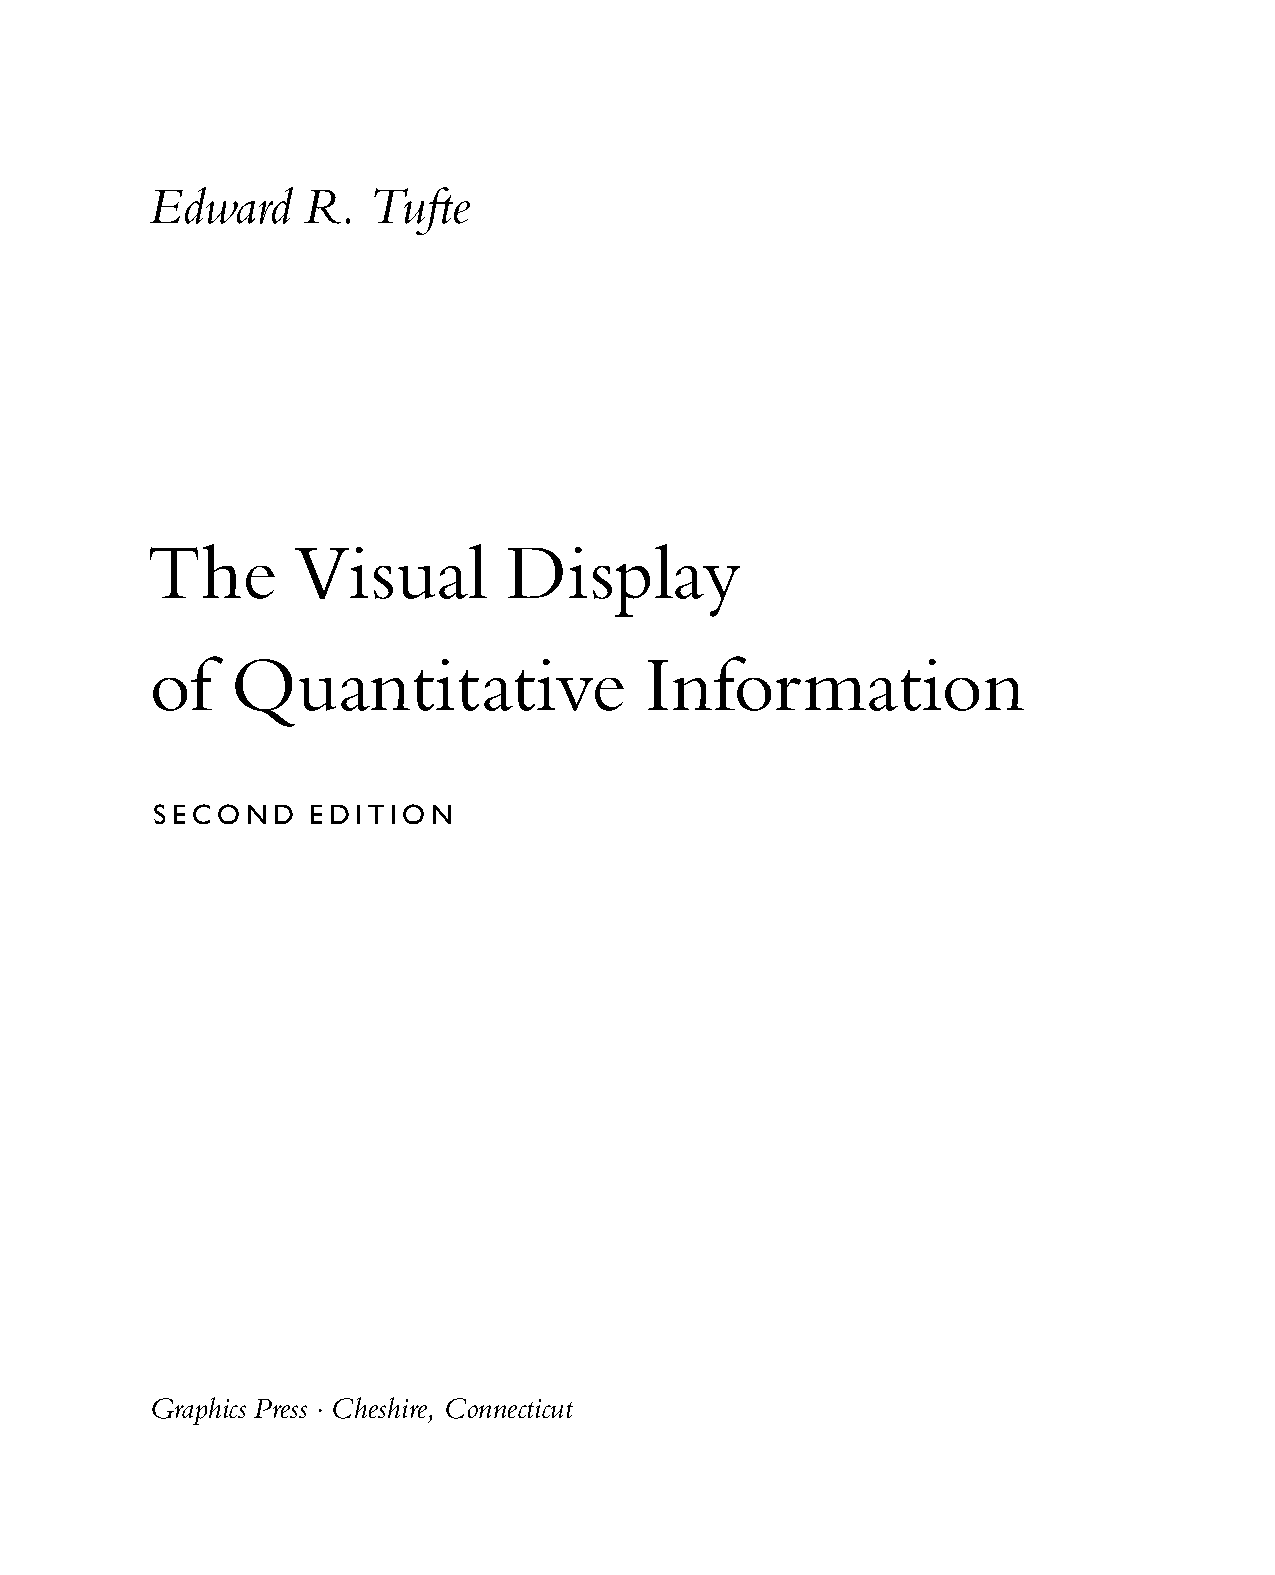
\includegraphics[width=0.45\linewidth]{graphics/vdqi-title.pdf}}
\hfill
\fbox{
\includegraphics[width=0.45\linewidth]{graphics/ei-title.pdf}}
\\\vspace{\baselineskip}
\fbox{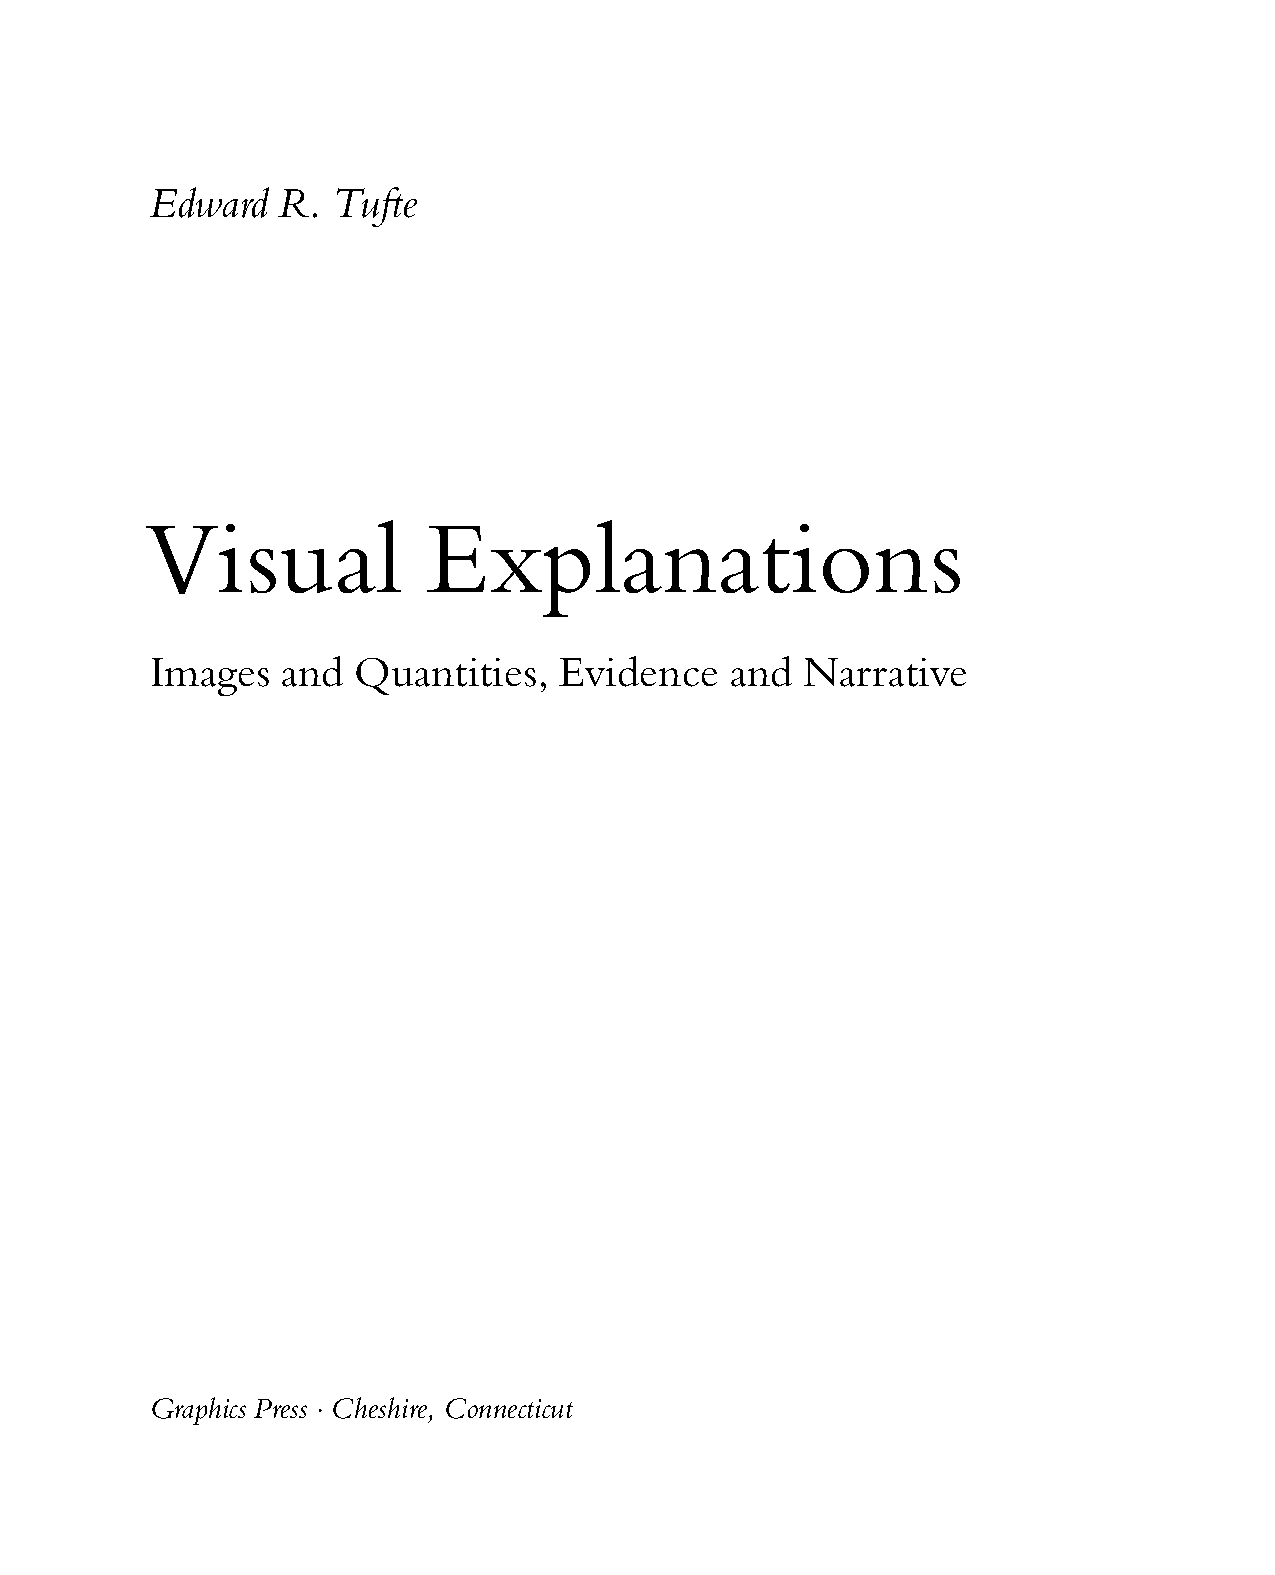
\includegraphics[width=0.45\linewidth]{graphics/ve-title.pdf}}
\hfill
\fbox{
\includegraphics[width=0.45\linewidth]{graphics/be-title.pdf}}
\end{figure*}

\newthought{The tables of contents} in Tufte's books give us our first
glimpse of the structure of the main matter.  \VDQI is split into two
parts, each containing some number of chapters.  His other three books only
contain chapters---they're not broken into parts.

\begin{figure*}[p]\index{table of contents}
\fbox{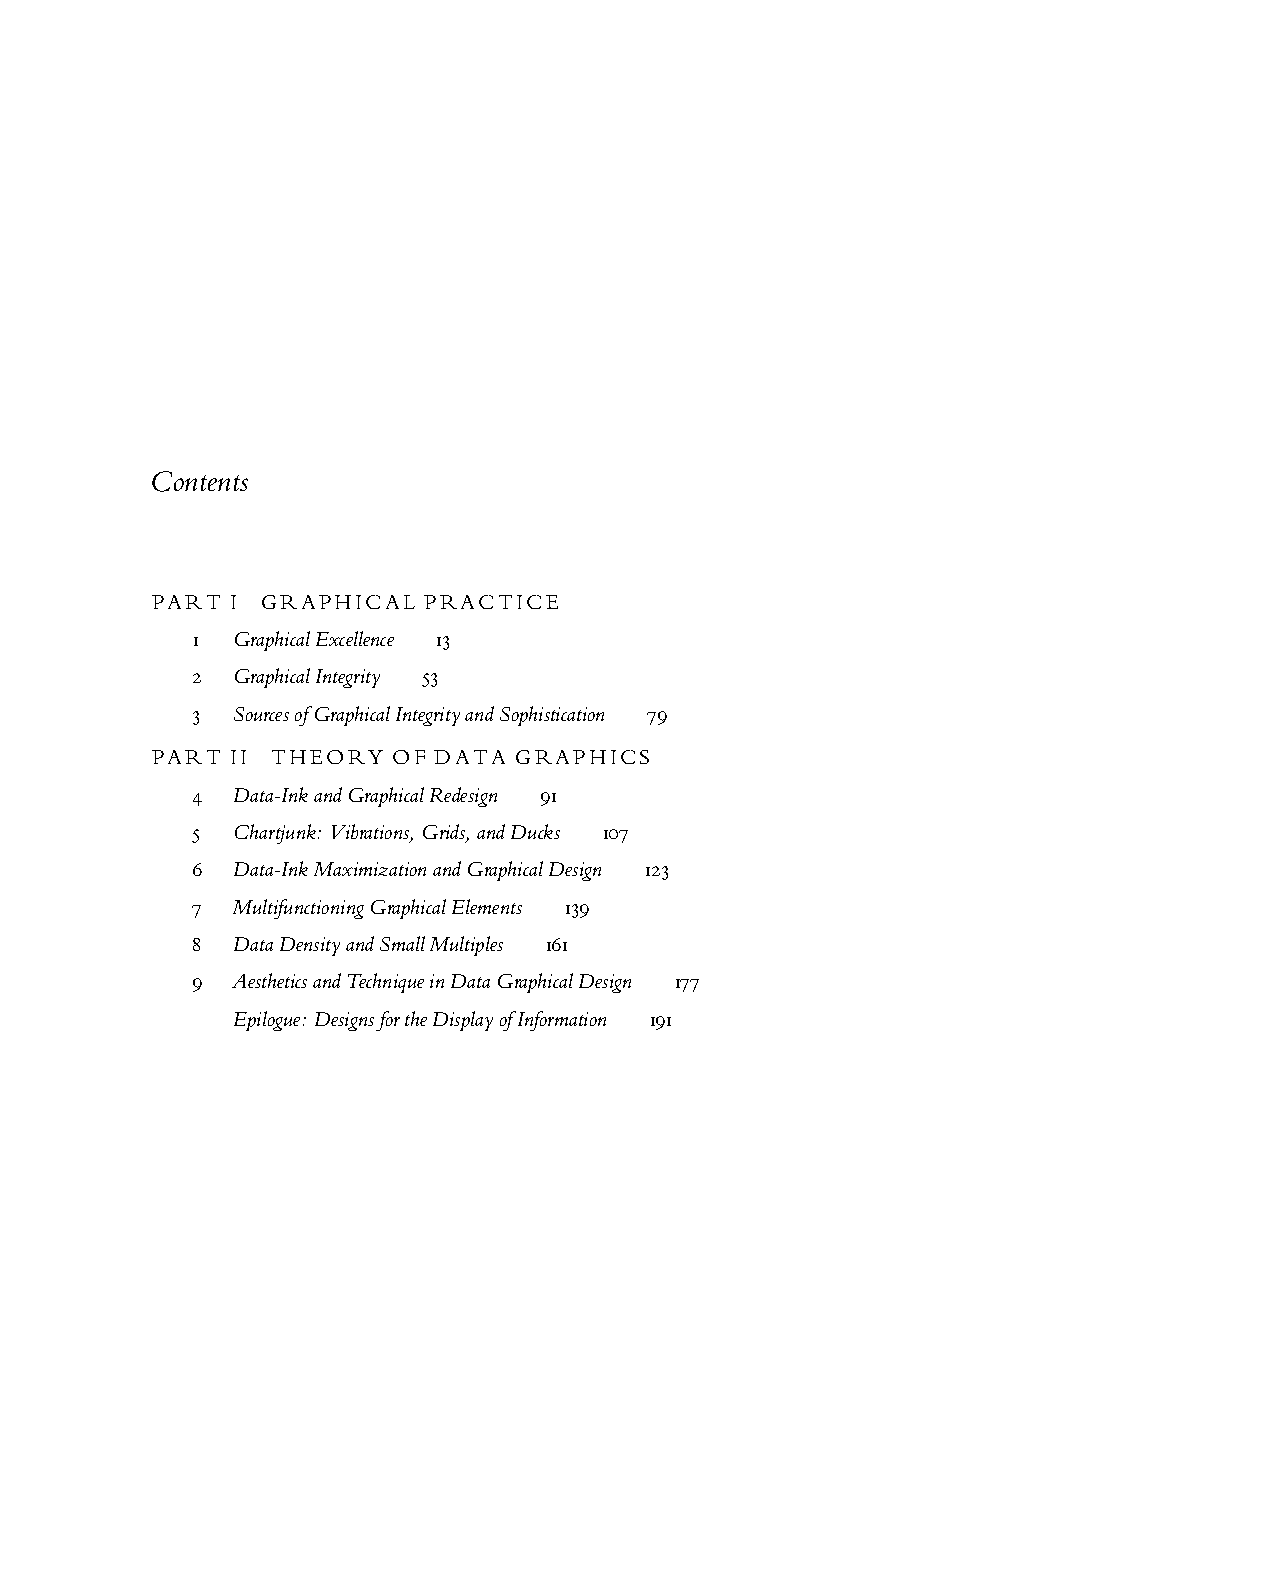
\includegraphics[width=0.45\linewidth]{graphics/vdqi-contents.pdf}}
\hfill
\fbox{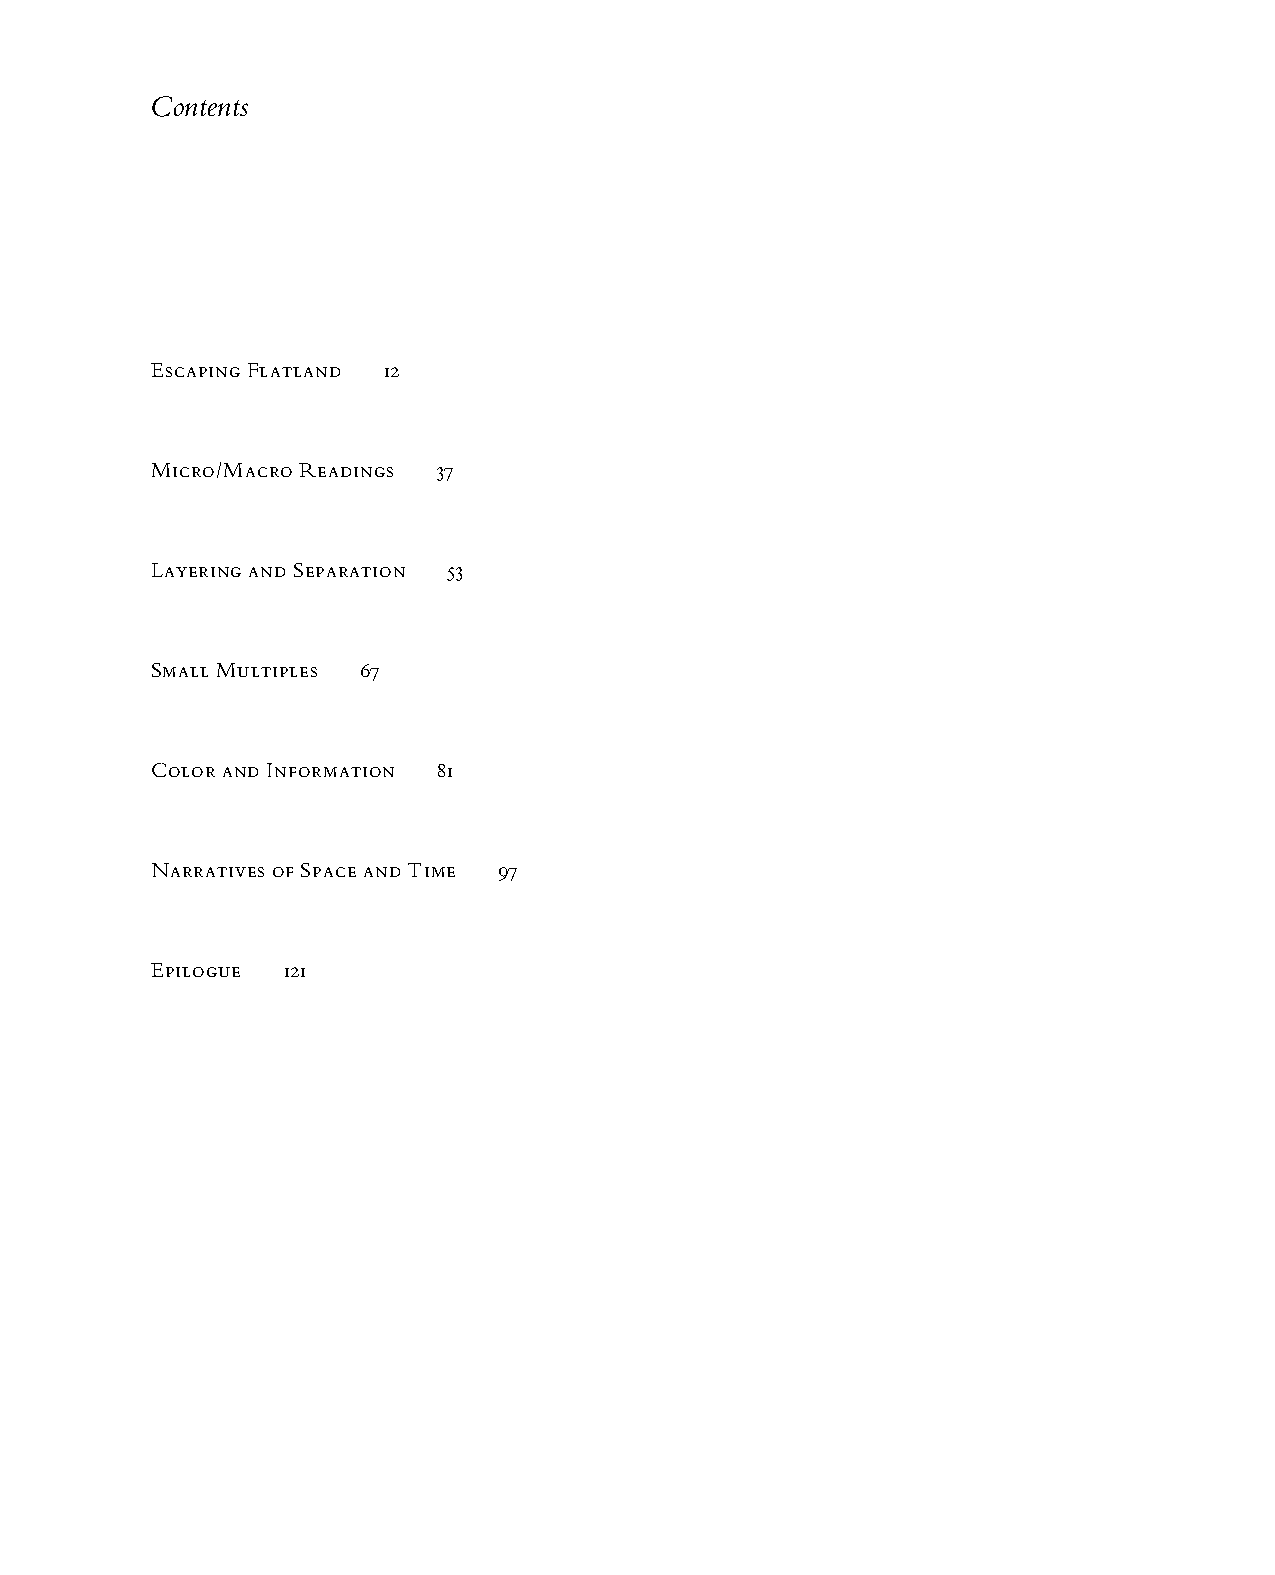
\includegraphics[width=0.45\linewidth]{graphics/ei-contents.pdf}}
\\\vspace{\baselineskip}
\fbox{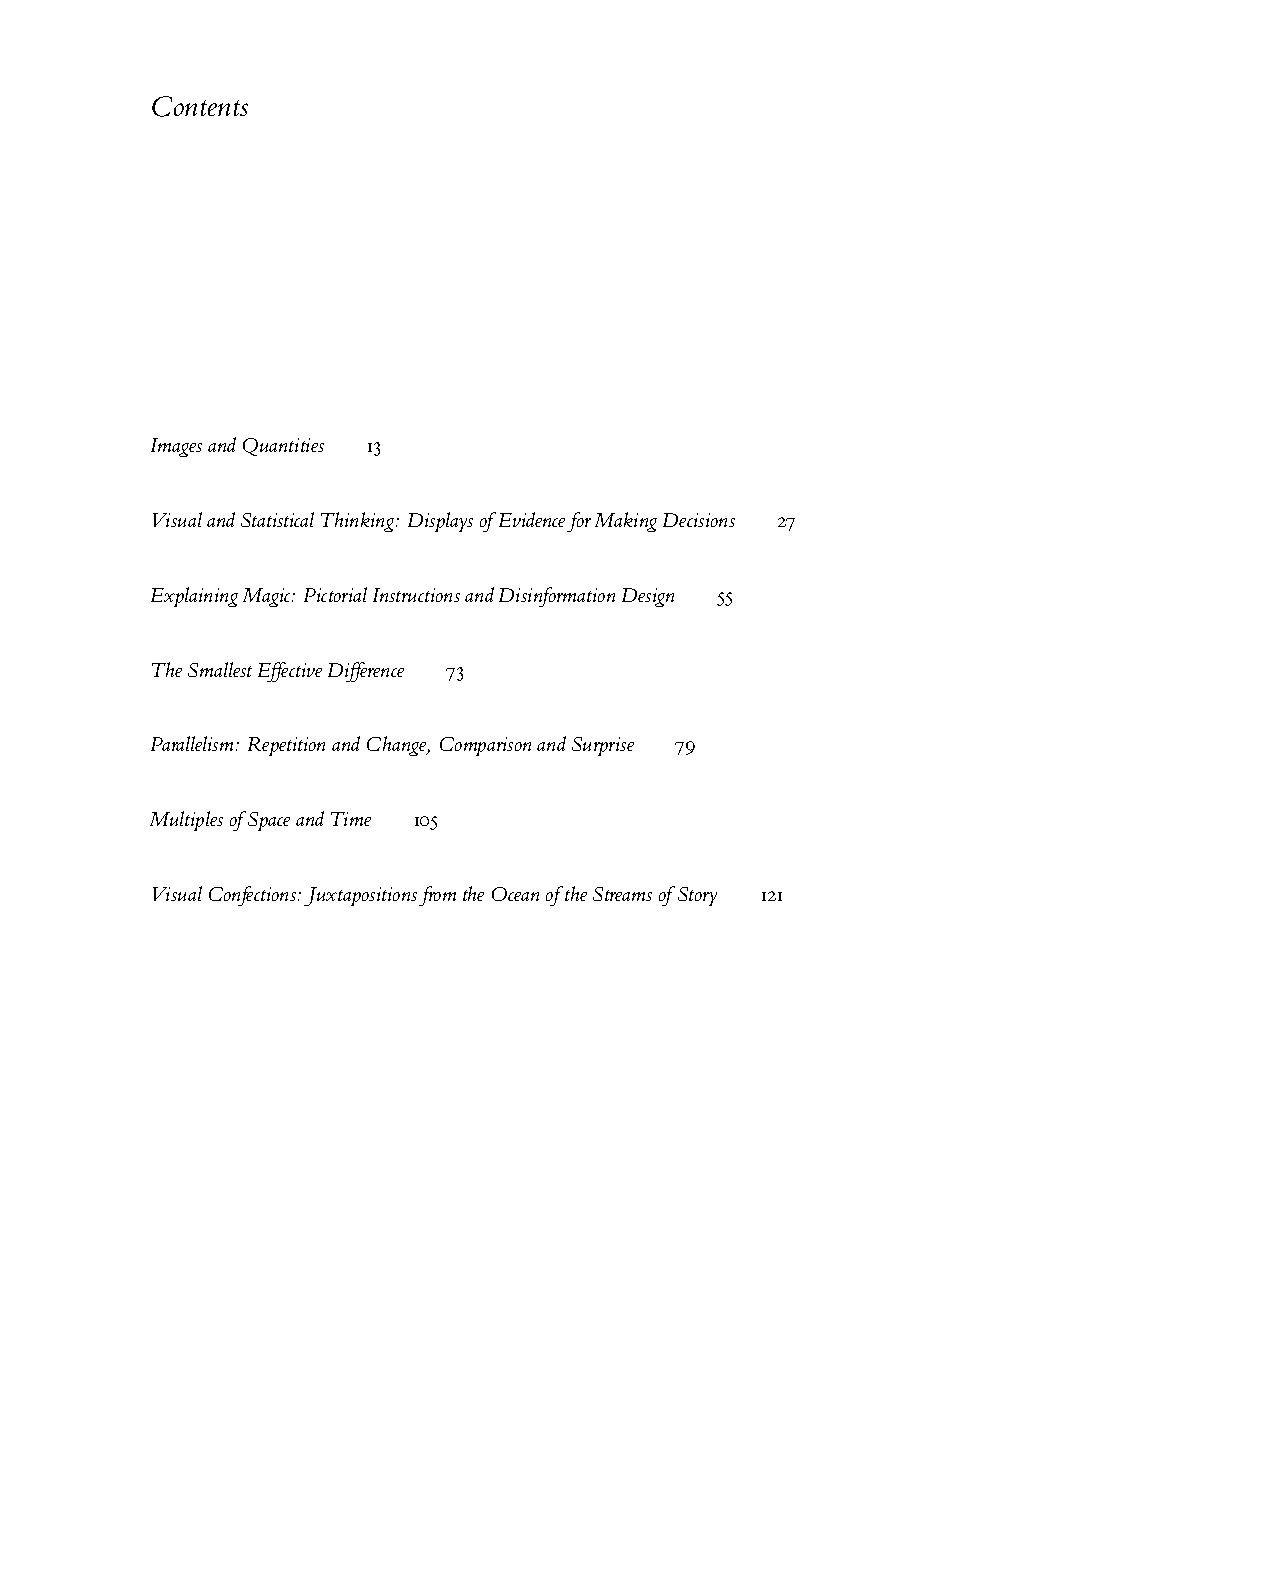
\includegraphics[width=0.45\linewidth]{graphics/ve-contents.pdf}}
\hfill
\fbox{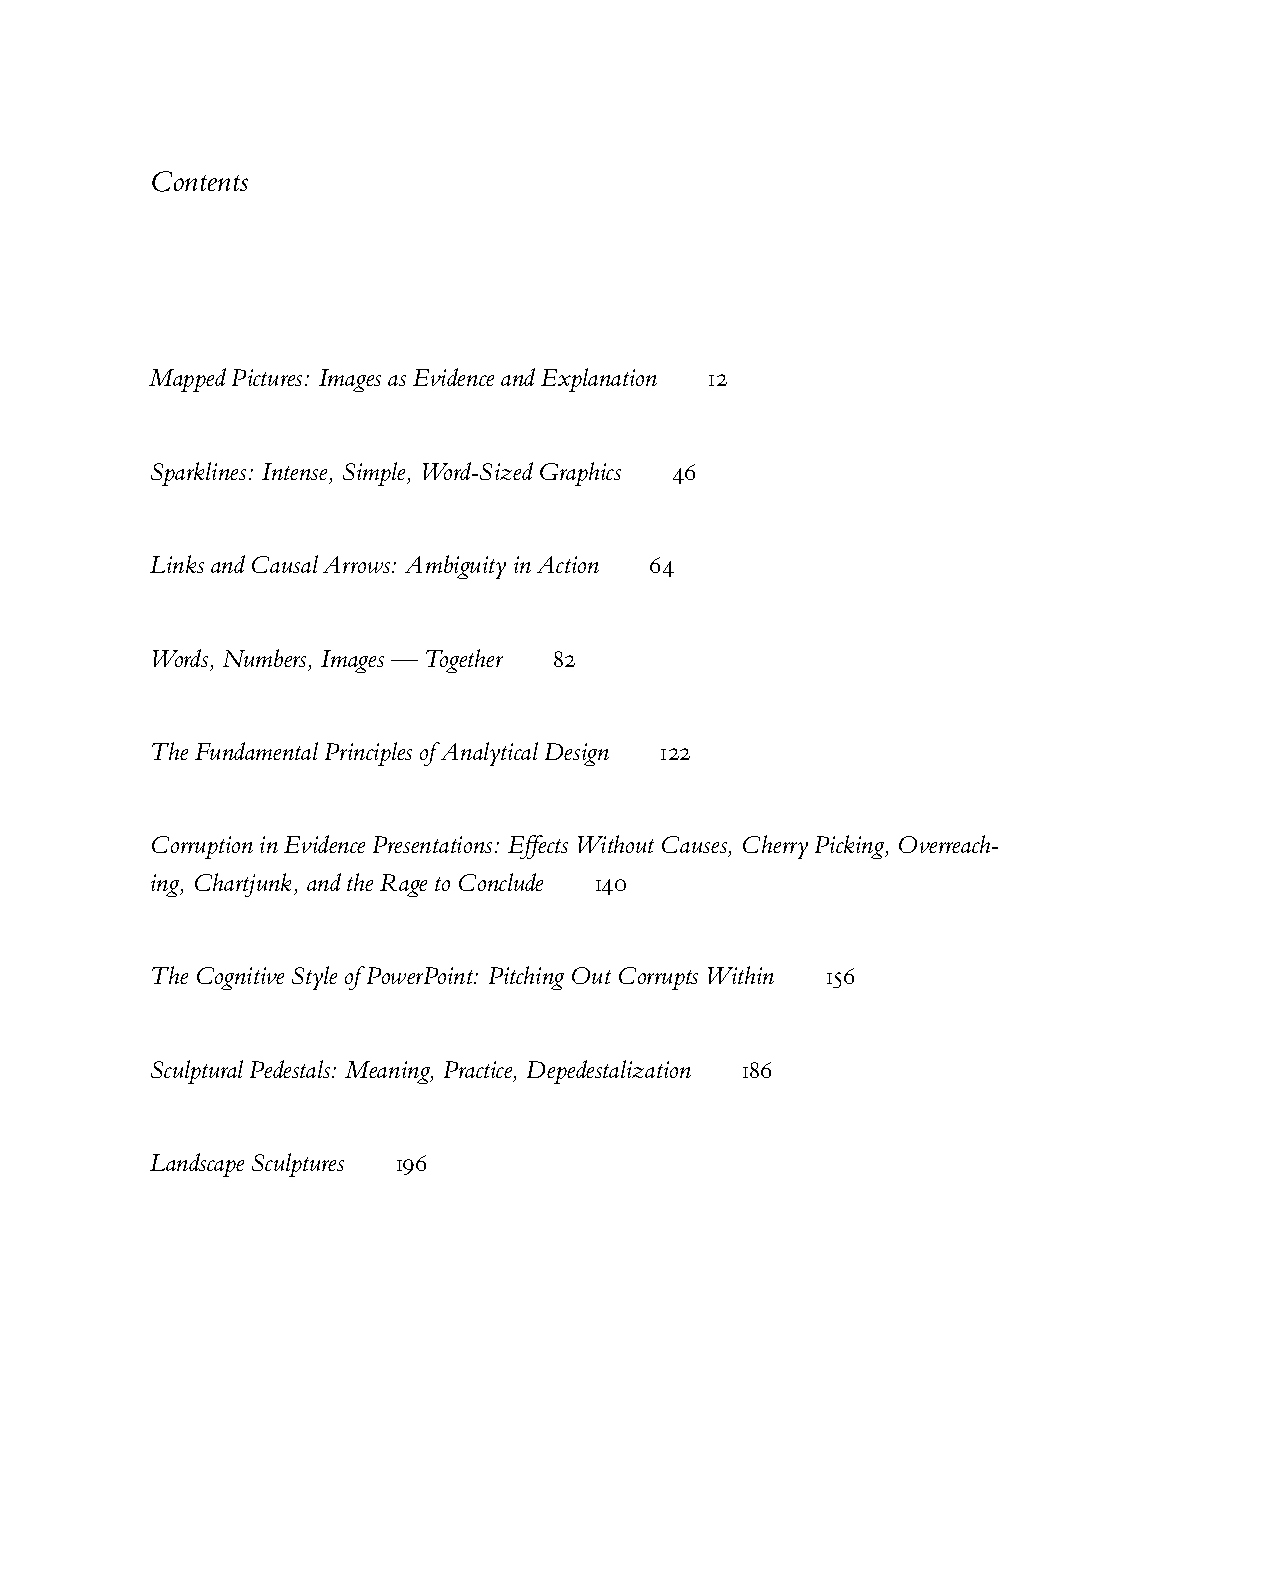
\includegraphics[width=0.45\linewidth]{graphics/be-contents.pdf}}
\end{figure*}


\section{Typefaces}\label{sec:typefaces1}\index{typefaces}
\index{fonts|see{typefaces}}

Tufte's books primarily use two typefaces: Bembo and Gill Sans.  Bembo is used
for the headings and body text, while Gill Sans is used for the title page and
opening epigraphs in \BE.

Since neither Bembo nor Gill Sans are available in default \LaTeX{}
installations, the \TL document classes default to using Palatino and
Helvetica, respectively.  In addition, the Bera Mono typeface is used for
\texttt{monospaced} type.

The following font sizes are defined by the \TL classes:

\begin{table}[h]\index{typefaces!sizes}
  \footnotesize%
  \begin{center}
    \begin{tabular}{lccl}
      \toprule
      \LaTeX{} size & Font size & Leading & Used for \\
      \midrule
      \verb+\tiny+         &  5 &  6 & sidenote numbers \\
      \verb+\scriptsize+   &  7 &  8 & \na \\
      \verb+\footnotesize+ &  8 & 10 & sidenotes, captions \\
      \verb+\small+        &  9 & 12 & quote, quotation, and verse environments \\
      \verb+\normalsize+   & 10 & 14 & body text \\
      \verb+\large+        & 11 & 15 & \textsc{b}-heads \\
      \verb+\Large+        & 12 & 16 & \textsc{a}-heads, \textsc{toc} entries, author, date \\
      \verb+\LARGE+        & 14 & 18 & handout title \\
      \verb+\huge+         & 20 & 30 & chapter heads \\
      \verb+\Huge+         & 24 & 36 & part titles \\
      \bottomrule
    \end{tabular}
  \end{center}
  \caption{A list of \LaTeX{} font sizes as defined by the \TL document classes.}
  \label{tab:font-sizes}
\end{table}

\section{Headings}\label{sec:headings1}\index{headings}

Tufte's books include the following heading levels: parts,
chapters,\sidenote{Parts and chapters are defined for the \texttt{tufte-book}
class only.}  sections, subsections, and paragraphs.  Not defined by default
are: sub-subsections and subparagraphs.

\begin{table}[h]
  \begin{center}
    \footnotesize%
    \begin{tabular}{lcr}
      \toprule
      Heading & Style & Size \\
      \midrule
      Part & roman & \measure{24}{36}{40} \\
      Chapter & italic & \measure{20}{30}{40} \\
      Section & italic & \measure{12}{16}{26} \\
      Subsection & italic & \measure{11}{15}{26} \\
      Paragraph & italic & 10/14 \\
      \bottomrule
    \end{tabular}
  \end{center}
  \caption{Heading styles used in \BE.}
  \label{tab:heading-styles}
\end{table}

\paragraph{Paragraph} Paragraph headings (as shown here) are introduced by
italicized text and separated from the main paragraph by a bit of space.

\section{Environments}

The following characteristics define the various environments:


\begin{table}[h]
  \begin{center}
    \footnotesize%
    \begin{tabular}{lcl}
      \toprule
      Environment & Font size & Notes \\
      \midrule
      Body text & \measure{10}{14}{26} & \\
      Block quote & \measure{9}{12}{24} & Block indent (left and right) by \unit[1]{pc} \\
      Sidenotes & \measure{8}{10}{12} & Sidenote number is set inline, followed by word space \\
      Captions & \measure{8}{10}{12} &  \\
      \bottomrule
    \end{tabular}
  \end{center}
  \caption{Environment styles used in \BE.}
  \label{tab:environment-styles}
\end{table}


\chapter[On the Use of the tufte-book Document Class]{On the Use of the \texttt{tufte-book} Document Class}
\label{ch:tufte-book}

The \TL document classes define a style similar to the
style Edward Tufte uses in his books and handouts.  Tufte's style is known
for its extensive use of sidenotes, tight integration of graphics with
text, and well-set typography.  This document aims to be at once a
demonstration of the features of the \TL document classes
and a style guide to their use.

\section{Page Layout}\label{sec:page-layout}
\subsection{Headings}\label{sec:headings}\index{headings}
This style provides \textsc{a}- and \textsc{b}-heads (that is,
\Verb|\section| and \Verb|\subsection|), demonstrated above.

If you need more than two levels of section headings, you'll have to define
them yourself at the moment; there are no pre-defined styles for anything below
a \Verb|\subsection|.  As Bringhurst points out in \textit{The Elements of
Typographic Style},\cite{Bringhurst2005} you should ``use as many levels of
headings as you need: no more, and no fewer.''

The \TL classes will emit an error if you try to use
\linebreak\Verb|\subsubsection| and smaller headings.

% let's start a new thought -- a new section
\newthought{In his later books},\cite{Tufte2006} Tufte
starts each section with a bit of vertical space, a non-indented paragraph,
and sets the first few words of the sentence in \textsc{small caps}.  To
accomplish this using this style, use the \doccmddef{newthought} command:
\begin{docspec}
  \doccmd{newthought}\{In his later books\}, Tufte starts\ldots
\end{docspec}


\section{Sidenotes}\label{sec:sidenotes}
One of the most prominent and distinctive features of this style is the
extensive use of sidenotes.  There is a wide margin to provide ample room
for sidenotes and small figures.  Any \doccmd{footnote}s will automatically
be converted to sidenotes.\footnote{This is a sidenote that was entered
using the \texttt{\textbackslash footnote} command.}  If you'd like to place ancillary
information in the margin without the sidenote mark (the superscript
number), you can use the \doccmd{marginnote} command.\marginnote{This is a
margin note.  Notice that there isn't a number preceding the note, and
there is no number in the main text where this note was written.}

The specification of the \doccmddef{sidenote} command is:
\begin{docspec}
  \doccmd{sidenote}[\docopt{number}][\docopt{offset}]\{\docarg{Sidenote text.}\}
\end{docspec}

Both the \docopt{number} and \docopt{offset} arguments are optional.  If you
provide a \docopt{number} argument, then that number will be used as the
sidenote number.  It will change the number of the current sidenote only and
will not affect the numbering sequence of subsequent sidenotes.

Sometimes a sidenote may run over the top of other text or graphics in the
margin space.  If this happens, you can adjust the vertical position of the
sidenote by providing a dimension in the \docopt{offset} argument.  Some
examples of valid dimensions are:
\begin{docspec}
  \ttfamily 1.0in \qquad 2.54cm \qquad 254mm \qquad 6\Verb|\baselineskip|
\end{docspec}
If the dimension is positive it will push the sidenote down the page; if the
dimension is negative, it will move the sidenote up the page.

While both the \docopt{number} and \docopt{offset} arguments are optional, they
must be provided in order.  To adjust the vertical position of the sidenote
while leaving the sidenote number alone, use the following syntax:
\begin{docspec}
  \doccmd{sidenote}[][\docopt{offset}]\{\docarg{Sidenote text.}\}
\end{docspec}
The empty brackets tell the \Verb|\sidenote| command to use the default
sidenote number.

If you \emph{only} want to change the sidenote number, however, you may
completely omit the \docopt{offset} argument:
\begin{docspec}
  \doccmd{sidenote}[\docopt{number}]\{\docarg{Sidenote text.}\}
\end{docspec}

The \doccmddef{marginnote} command has a similar \docarg{offset} argument:
\begin{docspec}
  \doccmd{marginnote}[\docopt{offset}]\{\docarg{Margin note text.}\}
\end{docspec}

\section{References}
References are placed alongside their citations as sidenotes,
as well.  This can be accomplished using the normal \doccmddef{cite}
command.\sidenote{The first paragraph of this document includes a citation.}

The complete list of references may also be printed automatically by using
the \doccmddef{bibliography} command.  (See the end of this document for an
example.)  If you do not want to print a bibliography at the end of your
document, use the \doccmddef{nobibliography} command in its place.  

To enter multiple citations at one location,\cite[-3\baselineskip]{Tufte2006,Tufte1990} you can
provide a list of keys separated by commas and the same optional vertical
offset argument: \Verb|\cite{Tufte2006,Tufte1990}|.  
\begin{docspec}
  \doccmd{cite}[\docopt{offset}]\{\docarg{bibkey1,bibkey2,\ldots}\}
\end{docspec}

\section{Figures and Tables}\label{sec:figures-and-tables}
Images and graphics play an integral role in Tufte's work.
In addition to the standard \docenvdef{figure} and \docenvdef{tabular} environments,
this style provides special figure and table environments for full-width
floats.

Full page--width figures and tables may be placed in \docenvdef{figure*} or
\docenvdef{table*} environments.  To place figures or tables in the margin,
use the \docenvdef{marginfigure} or \docenvdef{margintable} environments as follows
(see figure~\ref{fig:marginfig}):

\begin{marginfigure}%
  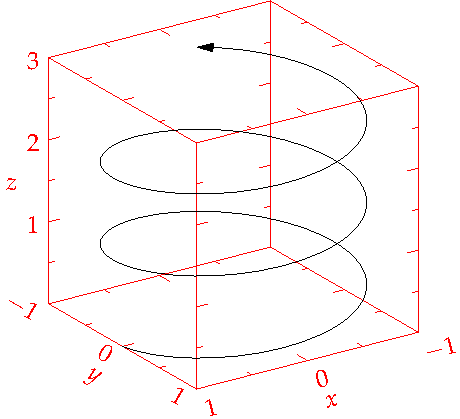
\includegraphics[width=\linewidth]{helix}
  \caption{This is a margin figure.  The helix is defined by 
    $x = \cos(2\pi z)$, $y = \sin(2\pi z)$, and $z = [0, 2.7]$.  The figure was
    drawn using Asymptote (\url{http://asymptote.sf.net/}).}
  \label{fig:marginfig}
\end{marginfigure}

\begin{docspec}
\textbackslash begin\{marginfigure\}\\
  \qquad\textbackslash includegraphics\{helix\}\\
  \qquad\textbackslash caption\{This is a margin figure.\}\\
  \qquad\textbackslash label\{fig:marginfig\}\\
\textbackslash end\{marginfigure\}\\
\end{docspec}

The \docenv{marginfigure} and \docenv{margintable} environments accept an optional parameter \docopt{offset} that adjusts the vertical position of the figure or table.  See the ``\nameref{sec:sidenotes}'' section above for examples.  The specifications are:
\begin{docspec}
  \textbackslash{begin\{marginfigure\}[\docopt{offset}]}\\
  \qquad\ldots\\
  \textbackslash{end\{marginfigure\}}\\
  \mbox{}\\
  \textbackslash{begin\{margintable\}[\docopt{offset}]}\\
  \qquad\ldots\\
  \textbackslash{end\{margintable\}}\\
\end{docspec}

Figure~\ref{fig:fullfig} is an example of the \docenv{figure*}
environment and figure~\ref{fig:textfig} is an example of the normal
\docenv{figure} environment.

\begin{figure*}[h]
  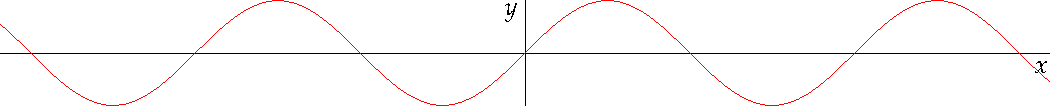
\includegraphics[width=\linewidth]{sine.pdf}%
  \caption{This graph shows $y = \sin x$ from about $x = [-10, 10]$.
  \emph{Notice that this figure takes up the full page width.}}%
  \label{fig:fullfig}%
\end{figure*}

\begin{figure}
  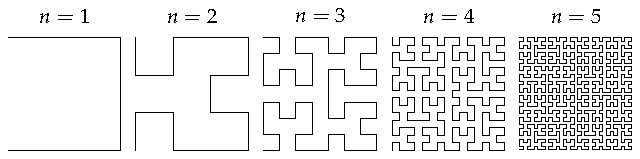
\includegraphics{hilbertcurves.pdf}
%  \checkparity This is an \pageparity\ page.%
  \caption[Hilbert curves of various degrees $n$.][6pt]{Hilbert curves of various degrees $n$. \emph{Notice that this figure only takes up the main textblock width.}}
  \label{fig:textfig}
  %\zsavepos{pos:textfig}
\end{figure}

As with sidenotes and marginnotes, a caption may sometimes require vertical
adjustment. The \doccmddef{caption} command now takes a second optional
argument that enables you to do this by providing a dimension \docopt{offset}.
You may specify the caption in any one of the following forms:
\begin{docspec}
  \doccmd{caption}\{\docarg{long caption}\}\\
  \doccmd{caption}[\docarg{short caption}]\{\docarg{long caption}\}\\
  \doccmd{caption}[][\docopt{offset}]\{\docarg{long caption}\}\\
  \doccmd{caption}[\docarg{short caption}][\docopt{offset}]%
                  \{\docarg{long caption}\}
\end{docspec}
A positive \docopt{offset} will push the caption down the page. The short
caption, if provided, is what appears in the list of figures/tables, otherwise
the ``long'' caption appears there. Note that although the arguments
\docopt{short caption} and \docopt{offset} are both optional, they must be
provided in order. Thus, to specify an \docopt{offset} without specifying a
\docopt{short caption}, you must include the first set of empty brackets
\Verb|[]|, which tell \doccmd{caption} to use the default ``long'' caption. As
an example, the caption to figure~\ref{fig:textfig} above was given in the form
\begin{docspec}
  \doccmd{caption}[Hilbert curves...][6pt]\{Hilbert curves...\}
\end{docspec}

Table~\ref{tab:normaltab} shows table created with the \docpkg{booktabs}
package.  Notice the lack of vertical rules---they serve only to clutter
the table's data.

\begin{table}[ht]
  \centering
  \fontfamily{ppl}\selectfont
  \begin{tabular}{ll}
    \toprule
    Margin & Length \\
    \midrule
    Paper width & \unit[8\nicefrac{1}{2}]{inches} \\
    Paper height & \unit[11]{inches} \\
    Textblock width & \unit[6\nicefrac{1}{2}]{inches} \\
    Textblock/sidenote gutter & \unit[\nicefrac{3}{8}]{inches} \\
    Sidenote width & \unit[2]{inches} \\
    \bottomrule
  \end{tabular}
  \caption{Here are the dimensions of the various margins used in the Tufte-handout class.}
  \label{tab:normaltab}
  %\zsavepos{pos:normaltab}
\end{table}

\newthought{Occasionally} \LaTeX{} will generate an error message:\label{err:too-many-floats}
\begin{docspec}
  Error: Too many unprocessed floats
\end{docspec}
\LaTeX{} tries to place floats in the best position on the page.  Until it's
finished composing the page, however, it won't know where those positions are.
If you have a lot of floats on a page (including sidenotes, margin notes,
figures, tables, etc.), \LaTeX{} may run out of ``slots'' to keep track of them
and will generate the above error.

\LaTeX{} initially allocates 18 slots for storing floats.  To work around this
limitation, the \TL document classes provide a \doccmddef{morefloats} command
that will reserve more slots.

The first time \doccmd{morefloats} is called, it allocates an additional 34
slots.  The second time \doccmd{morefloats} is called, it allocates another 26
slots.

The \doccmd{morefloats} command may only be used two times.  Calling it a
third time will generate an error message.  (This is because we can't safely
allocate many more floats or \LaTeX{} will run out of memory.)

If, after using the \doccmd{morefloats} command twice, you continue to get the
\texttt{Too many unprocessed floats} error, there are a couple things you can
do.

The \doccmddef{FloatBarrier} command will immediately process all the floats
before typesetting more material.  Since \doccmd{FloatBarrier} will start a new
paragraph, you should place this command at the beginning or end of a
paragraph.

The \doccmddef{clearpage} command will also process the floats before
continuing, but instead of starting a new paragraph, it will start a new page.

You can also try moving your floats around a bit: move a figure or table to the
next page or reduce the number of sidenotes.  (Each sidenote actually uses
\emph{two} slots.)

After the floats have placed, \LaTeX{} will mark those slots as unused so they
are available for the next page to be composed.

\section{Captions}
You may notice that the captions are sometimes misaligned.
Due to the way \LaTeX's float mechanism works, we can't know for sure where it
decided to put a float. Therefore, the \TL document classes provide commands to
override the caption position.

\paragraph{Vertical alignment} To override the vertical alignment, use the
\doccmd{setfloatalignment} command inside the float environment.  For
example:

\begin{fullwidth}
\begin{docspec}
  \textbackslash begin\{figure\}[btp]\\
  \qquad \textbackslash includegraphics\{sinewave\}\\
  \qquad \textbackslash caption\{This is an example of a sine wave.\}\\
  \qquad \textbackslash label\{fig:sinewave\}\\
  \qquad \hlred{\textbackslash setfloatalignment\{b\}\% forces caption to be bottom-aligned}\\
  \textbackslash end\{figure\}
\end{docspec}
\end{fullwidth}

\noindent The syntax of the \doccmddef{setfloatalignment} command is:

\begin{docspec}
  \doccmd{setfloatalignment}\{\docopt{pos}\}
\end{docspec}

\noindent where \docopt{pos} can be either \texttt{b} for bottom-aligned
captions, or \texttt{t} for top-aligned captions.

\paragraph{Horizontal alignment}\label{par:overriding-horizontal}
To override the horizontal alignment, use either the \doccmd{forceversofloat}
or the \doccmd{forcerectofloat} command inside of the float environment.  For
example:

\begin{fullwidth}
\begin{docspec}
  \textbackslash begin\{figure\}[btp]\\
  \qquad \textbackslash includegraphics\{sinewave\}\\
  \qquad \textbackslash caption\{This is an example of a sine wave.\}\\
  \qquad \textbackslash label\{fig:sinewave\}\\
  \qquad \hlred{\textbackslash forceversofloat\% forces caption to be set to the left of the float}\\
  \textbackslash end\{figure\}
\end{docspec}
\end{fullwidth}

The \doccmddef{forceversofloat} command causes the algorithm to assume the
float has been placed on a verso page---that is, a page on the left side of a
two-page spread.  Conversely, the \doccmddef{forcerectofloat} command causes
the algorithm to assume the float has been placed on a recto page---that is, a
page on the right side of a two-page spread.


\section{Full-width text blocks}

In addition to the new float types, there is a \docenvdef{fullwidth}
environment that stretches across the main text block and the sidenotes
area.

\begin{Verbatim}
\begin{fullwidth}
Lorem ipsum dolor sit amet...
\end{fullwidth}
\end{Verbatim}

\begin{fullwidth}
\small\itshape\lipsum[1]
\end{fullwidth}

\section{Typography}\label{sec:typography}

\subsection{Typefaces}\label{sec:typefaces}\index{typefaces}
If the Palatino, \textsf{Helvetica}, and \texttt{Bera Mono} typefaces are installed, this style
will use them automatically.  Otherwise, we'll fall back on the Computer Modern
typefaces.

\subsection{Letterspacing}\label{sec:letterspacing}
This document class includes two new commands and some improvements on
existing commands for letterspacing.

When setting strings of \allcaps{ALL CAPS} or \smallcaps{small caps}, the
letter\-spacing---that is, the spacing between the letters---should be
increased slightly.\cite{Bringhurst2005}  The \doccmddef{allcaps} command has proper letterspacing for
strings of \allcaps{FULL CAPITAL LETTERS}, and the \doccmddef{smallcaps} command
has letterspacing for \smallcaps{small capital letters}.  These commands
will also automatically convert the case of the text to upper- or
lowercase, respectively.

The \doccmddef{textsc} command has also been redefined to include
letterspacing.  The case of the \doccmd{textsc} argument is left as is,
however.  This allows one to use both uppercase and lowercase letters:
\textsc{The Initial Letters Of The Words In This Sentence Are Capitalized.}



\section{Document Class Options}\label{sec:options}

\index{class options|(}
The \doccls{tufte-book} class is based on the \LaTeX\ \doccls{book}
document class.  Therefore, you can pass any of the typical book
options.  There are a few options that are specific to the
\doccls{tufte-book} document class, however.

The \docclsoptdef{a4paper} option will set the paper size to \smallcaps{A4} instead of
the default \smallcaps{US} letter size.

The \docclsoptdef{sfsidenotes} option will set the sidenotes and title block in a 
\textsf{sans serif} typeface instead of the default roman.

The \docclsoptdef{twoside} option will modify the running heads so that the page
number is printed on the outside edge (as opposed to always printing the page
number on the right-side edge in \docclsoptdef{oneside} mode).  

The \docclsoptdef{symmetric} option typesets the sidenotes on the outside edge of
the page.  This is how books are traditionally printed, but is contrary to
Tufte's book design which sets the sidenotes on the right side of the page.
This option implicitly sets the \docclsopt{twoside} option.

The \docclsoptdef{justified} option sets all the text fully justified (flush left
and right).  The default is to set the text ragged right.  
The body text of Tufte's books are set ragged right.  This prevents
needless hyphenation and makes it easier to read the text in the slightly
narrower column.

The \docclsoptdef{bidi} option loads the \docpkg{bidi} package which is used with
\tXeLaTeX\ to typeset bi-directional text.  Since the \docpkg{bidi}
package needs to be loaded before the sidenotes and cite commands are defined,
it can't be loaded in the document preamble.

The \docclsoptdef{debug} option causes the \TL classes to output debug
information to the log file which is useful in troubleshooting bugs.  It will
also cause the graphics to be replaced by outlines.

The \docclsoptdef{nofonts} option prevents the \TL classes from
automatically loading the Palatino and Helvetica typefaces.  You should use
this option if you wish to load your own fonts.  If you're using \tXeLaTeX, this
option is implied (i.e., the Palatino and Helvetica fonts aren't loaded if you
use \tXeLaTeX).  

The \docclsoptdef{nols} option inhibits the letterspacing code.  The \TL\
classes try to load the appropriate letterspacing package (either pdf\TeX's
\docpkg{letterspace} package or the \docpkg{soul} package).  If you're using
\tXeLaTeX\ with \docpkg{fontenc}, however, you should configure your own
letterspacing.  

The \docclsoptdef{notitlepage} option causes \doccmd{maketitle} to generate a title
block instead of a title page.  The \doccls{book} class defaults to a title
page and the \doccls{handout} class defaults to the title block.  There is an
analogous \docclsoptdef{titlepage} option that forces \doccmd{maketitle} to
generate a full title page instead of the title block.

The \docclsoptdef{notoc} option suppresses \TL's custom table of contents
(\textsc{toc}) design.  The current \textsc{toc} design only shows unnumbered
chapter titles; it doesn't show sections or subsections.  The \docclsopt{notoc}
option will revert to \LaTeX's \textsc{toc} design.

The \docclsoptdef{nohyper} option prevents the \docpkg{hyperref} package from
being loaded.  The default is to load the \docpkg{hyperref} package and use the
\doccmd{title} and \doccmd{author} contents as metadata for the generated
\textsc{pdf}.

\index{class options|)}



\chapter[Customizing Tufte-LaTeX]{Customizing \TL}
\label{ch:customizing}

The \TL document classes are designed to closely emulate Tufte's book
design by default.  However, each document is different and you may encounter
situations where the default settings are insufficient.  This chapter explores
many of the ways you can adjust the \TL document classes to better fit
your needs.

\section{File Hooks}
\label{sec:filehooks}

\index{file hooks|(}
If you create many documents using the \TL classes, it's easier to
store your customizations in a separate file instead of copying them into the
preamble of each document.  The \TL classes provide three file hooks:
\docfilehook{tufte-common-local.tex}{common}, \docfilehook{tufte-book-local.tex}{book}, and
\docfilehook{tufte-handout-local.tex}{handout}.\sloppy

\begin{description}
  \item[\docfilehook{tufte-common-local.tex}{common}]
    If this file exists, it will be loaded by all of the \TL document
    classes just prior to any document-class-specific code.  If your
    customizations or code should be included in both the book and handout
    classes, use this file hook.
  \item[\docfilehook{tufte-book-local.tex}{book}] 
    If this file exists, it will be loaded after all of the common and
    book-specific code has been read.  If your customizations apply only to the
    book class, use this file hook.
  \item[\docfilehook{tufte-common-handout.tex}{handout}] 
    If this file exists, it will be loaded after all of the common and
    handout-specific code has been read.  If your customizations apply only to
    the handout class, use this file hook.
\end{description}

\index{file hooks|)}

\section{Numbered Section Headings}
\label{sec:numbered-sections}
\index{headings!numbered}

While Tufte dispenses with numbered headings in his books, if you require them,
they can be anabled by changing the value of the \doccounter{secnumdepth}
counter.  From the table below, select the heading level at which numbering
should stop and set the \doccounter{secnumdepth} counter to that value.  For
example, if you want parts and chapters numbered, but don't want numbering for
sections or subsections, use the command:
\begin{docspec}
  \doccmd{setcounter}\{secnumdepth\}\{0\}
\end{docspec}

The default \doccounter{secnumdepth} for the \TL document classes is $-1$.

\begin{table}
  \footnotesize
  \begin{center}
    \begin{tabular}{lr}
      \toprule
      Heading level & Value \\
      \midrule
      Part (in \doccls{tufte-book}) & $-1$ \\
      Part (in \doccls{tufte-handout}) & $0$ \\
      Chapter (only in \doccls{tufte-book}) & $0$ \\
      Section & $1$ \\
      Subsection & $2$ \\
      Subsubsection & $3$ \\
      Paragraph & $4$ \\
      Subparagraph & $5$ \\
      \bottomrule
    \end{tabular}
  \end{center}
  \caption{Heading levels used with the \texttt{secnumdepth} counter.}
\end{table}

\section{Changing the Paper Size}
\label{sec:paper-size}

The \TL classes currently only provide three paper sizes: \textsc{a4},
\textsc{b5}, and \textsc{us} letter.  To specify a different paper size (and/or
margins), use the \doccmd[geometry]{geometry} command in the preamble of your
document (or one of the file hooks).  The full documentation of the
\doccmd{geometry} command may be found in the \docpkg{geometry} package
documentation.\cite{pkg-geometry}


\section{Customizing Marginal Material}
\label{sec:marginal-material}

Marginal material includes sidenotes, citations, margin notes, and captions.
Normally, the justification of the marginal material follows the justification
of the body text.  If you specify the \docclsopt{justified} document class
option, all of the margin material will be fully justified as well.  If you
don't specify the \docclsopt{justified} option, then the marginal material will
be set ragged right.

You can set the justification of the marginal material separately from the body
text using the following document class options: \docclsopt{sidenote},
\docclsopt{marginnote}, \docclsopt{caption}, \docclsopt{citation}, and
\docclsopt{marginals}.  Each option refers to its obviously corresponding
marginal material type.  The \docclsopt{marginals} option simultaneously sets
the justification on all four marginal material types.

Each of the document class options takes one of five justification types:
\begin{description}
  \item[\docclsopt{justified}] Fully justifies the text (sets it flush left and
    right).
  \item[\docclsopt{raggedleft}] Sets the text ragged left, regardless of which
    page it falls on.
  \item[\docclsopt{raggedright}] Sets the text ragged right, regardless of
    which page it falls on.
  \item[\doccls{raggedouter}] Sets the text ragged left if it falls on the
    left-hand (verso) page of the spread and otherwise sets it ragged right.
    This is useful in conjunction with the \docclsopt{symmetric} document class
    option.
  \item[\docclsopt{auto}] If the \docclsopt{justified} document class option
    was specified, then set the text fully justified; otherwise the text is set
    ragged right.  This is the default justification option if one is not
    explicitly specified.
\end{description}

\noindent For example, 
\begin{docspec}
  \doccmdnoindex{documentclass}[symmetric,justified,marginals=raggedouter]\{tufte-book\}
\end{docspec}
will set the body text of the document to be fully justified and all of the
margin material (sidenotes, margin notes, captions, and citations) to be flush
against the body text with ragged outer edges.

\newthought{The font and style} of the marginal material may also be modified using the following commands:

\begin{docspec}
  \doccmd{setsidenotefont}\{\docopt{font commands}\}\\
  \doccmd{setcaptionfont}\{\docopt{font commands}\}\\
  \doccmd{setmarginnotefont}\{\docopt{font commands}\}\\
  \doccmd{setcitationfont}\{\docopt{font commands}\}
\end{docspec}

The \doccmddef{setsidenotefont} sets the font and style for sidenotes, the
\doccmddef{setcaptionfont} for captions, the \doccmddef{setmarginnotefont} for
margin notes, and the \doccmddef{setcitationfont} for citations.  The
\docopt{font commands} can contain font size changes (e.g.,
\doccmdnoindex{footnotesize}, \doccmdnoindex{Huge}, etc.), font style changes (e.g.,
\doccmdnoindex{sffamily}, \doccmdnoindex{ttfamily}, \doccmdnoindex{itshape}, etc.), color changes (e.g.,
\doccmdnoindex{color}\texttt{\{blue\}}), and many other adjustments.

If, for example, you wanted the captions to be set in italic sans serif, you could use:
\begin{docspec}
  \doccmd{setcaptionfont}\{\doccmdnoindex{itshape}\doccmdnoindex{sffamily}\}
\end{docspec}

\chapter{Compatibility Issues}
\label{ch:compatibility}

When switching an existing document from one document class to a \TL document class, a few changes to the document may have to be made.

\section{Converting from \doccls{article} to \doccls{tufte-handout}}

The following \doccls{article} class options are unsupported: \docclsopt{10pt}, \docclsopt{11pt}, \docclsopt{12pt}, \docclsopt{a5paper}, \docclsopt{b5paper}, \docclsopt{executivepaper}, \docclsopt{legalpaper}, \docclsopt{landscape}, \docclsopt{onecolumn}, and \doccls{twocolumn}.

The following headings are not supported: \doccmd{subsubsection} and \doccmd{subparagraph}.

\section{Converting from \doccls{book} to \doccls{tufte-book}}

The following \doccls{report} class options are unsupported: \docclsopt{10pt}, \docclsopt{11pt}, \docclsopt{12pt}, \docclsopt{a5paper}, \docclsopt{b5paper}, \docclsopt{executivepaper}, \docclsopt{legalpaper}, \docclsopt{landscape}, \docclsopt{onecolumn}, and \doccls{twocolumn}.

The following headings are not supported: \doccmd{subsubsection} and \doccmd{subparagraph}.



\chapter{Troubleshooting and Support}
\label{ch:troubleshooting}

\section{\TL Website}\label{sec:website}
The website for the \TL packages is located at
\url{https://github.com/Tufte-LaTeX/tufte-latex}.  On our website, you'll find
links to our \smallcaps{svn} repository, mailing lists, bug tracker, and documentation.

\section{\TL Mailing Lists}\label{sec:mailing-lists}
There are two mailing lists for the \TL project:

\paragraph{Discussion list}
The \texttt{tufte-latex} discussion list is for asking questions, getting
assistance with problems, and help with troubleshooting.  Release announcements
are also posted to this list.  You can subscribe to the \texttt{tufte-latex}
discussion list at \url{http://groups.google.com/group/tufte-latex}.

\paragraph{Commits list}
The \texttt{tufte-latex-commits} list is a read-only mailing list.  A message
is sent to the list any time the \TL code has been updated.  If you'd like to
keep up with the latest code developments, you may subscribe to this list.  You
can subscribe to the \texttt{tufte-latex-commits} mailing list at
\url{http://groups.google.com/group/tufte-latex-commits}.

\section{Getting Help}\label{sec:getting-help}
If you've encountered a problem with one of the \TL document classes, have a
question, or would like to report a bug, please send an email to our
mailing list or visit our website.

To help us troubleshoot the problem more quickly, please try to compile your
document using the \docclsopt{debug} class option and send the generated
\texttt{.log} file to the mailing list with a brief description of the problem.



\section{Errors, Warnings, and Informational Messages}\label{sec:tl-messages}
The following is a list of all of the errors, warnings, and other messages generated by the \TL classes and a brief description of their meanings.
\index{error messages}\index{warning messages}\index{debug messages}

% Errors
\docmsg{Error: \doccmd{subparagraph} is undefined by this class.}{%
The \doccmd{subparagraph} command is not defined in the \TL document classes.
If you'd like to use the \doccmd{subparagraph} command, you'll need to redefine
it yourself.  See the ``Headings'' section on page~\pageref{sec:headings} for a
description of the heading styles available in the \TL document classes.}

\docmsg{Error: \doccmd{subsubsection} is undefined by this class.}{%
The \doccmd{subsubsection} command is not defined in the \TL document classes.
If you'd like to use the \doccmd{subsubsection} command, you'll need to
redefine it yourself.  See the ``Headings'' section on
page~\pageref{sec:headings} for a description of the heading styles available
in the \TL document classes.}

\docmsg{Error: You may only call \doccmd{morefloats} twice. See the\par\noindent\ \ \ \ \ \ \ \ Tufte-LaTeX documentation for other workarounds.}{%
\LaTeX{} allocates 18 slots for storing floats.  The first time
\doccmd{morefloats} is called, it allocates an additional 34 slots.  The second
time \doccmd{morefloats} is called, it allocates another 26 slots.

The \doccmd{morefloats} command may only be called two times.  Calling it a
third time will generate this error message.  See
page~\pageref{err:too-many-floats} for more information.}

% Warnings
\docmsg{Warning: Option `\docopt{class option}' is not supported -{}- ignoring option.}{%
This warning appears when you've tried to use \docopt{class option} with a \TL
document class, but \docopt{class option} isn't supported by the \TL document
class.  In this situation, \docopt{class option} is ignored.}

% Info / Debug messages
\docmsg{Info: The `\docclsopt{symmetric}' option implies `\docclsopt{twoside}'}{%
You specified the \docclsopt{symmetric} document class option.  This option automatically forces the \docclsopt{twoside} option as well.  See page~\pageref{clsopt:symmetric} for more information on the \docclsopt{symmetric} class option.}


\section{Package Dependencies}\label{sec:dependencies}
The following is a list of packages that the \TL document
classes rely upon.  Packages marked with an asterisk are optional.
\begin{multicols}{2}
\begin{itemize}
  \item xifthen
  \item ifpdf*
  \item ifxetex*
  \item hyperref
  \item geometry
  \item ragged2e
  \item chngpage \emph{or} changepage
  \item paralist
  \item textcase
  \item soul*
  \item letterspace*
  \item setspace
  \item natbib \emph{and} bibentry
  \item optparams
  \item placeins
  \item mathpazo*
  \item helvet*
  \item fontenc
  \item beramono*
  \item fancyhdr
  \item xcolor
  \item textcomp
  \item titlesec
  \item titletoc
\end{itemize}
\end{multicols}




%%
% The back matter contains appendices, bibliographies, indices, glossaries, etc.







\backmatter

\bibliography{sample-handout}
\bibliographystyle{plainnat}


\printindex

\end{document}

